% ----- LIVECOMS ARTICLE TEMPLATE FOR BEST PRACTICES GUIDE -----
% ADAPTED FROM ELIFE ARTICLE TEMPLATE (8/10/2017)
% ----- -------- ------- -------- --- ---- --------- ----- -----

% ----- PREAMBLE -----
\documentclass[9pt,tutorial]{livecoms}
% 'onehalfspacing' : 1.5 line spacing
% 'doublespacing' : 2.0 line spacing
% 'lineno' : add line numbers
% 'pubversion' : add citation and publication information to footer, when the DOI is assigned and the article is added to a live issue.

% USER PACKAGES
\usepackage{tikz}
\usepackage{xtab}
\usepackage{xurl}
\usepackage{float}
\usepackage{xcolor}
\usepackage{amsmath}
\usepackage{amssymb}
\usepackage{ltablex}
\usepackage{siunitx}
\usepackage{booktabs}
\usepackage{enumitem}
\usepackage{fancyhdr}
\usepackage{graphicx}
\usepackage{hyperref}
\usepackage{listings}
\usepackage{placeins}
\usepackage{tabularx}
\usepackage{subcaption}
\usepackage{inconsolata}
\usepackage[english]{babel}
\usepackage[utf8]{inputenc}
\usepackage[plain]{fancyref}
\usepackage[euler]{textgreek}
\usepackage[font=small,labelfont=bf]{caption}

% USER LIBRARIES
\usetikzlibrary{backgrounds}
\usetikzlibrary{calc}

% JOURNAL PACKAGES
\usepackage[version=4]{mhchem}
\usepackage{siunitx}
\DeclareSIUnit\Molar{M}
\usepackage[italic]{mathastext}
\graphicspath{{figures/}}

% DEFINE version number of this Tutorial
\newcommand{\versionnumber}{1.0}

% DEFINE githubrepository for this articel
\newcommand{\githubrepository}{\url{https://github.com/Foly93/MD_FromBasicsToApplication}}  

% DEFINITION OF CODEBOX VIA LISTINGS PACKAGE
\lstset{showstringspaces = false,
        framexleftmargin = 8pt,
        backgroundcolor = \color{light-gray},
        framextopmargin = 10pt,
        keywordstyle = \color{blue},
        commentstyle = \color{red},
        xleftmargin = 13pt,
        basicstyle = \footnotesize\ttfamily,
        breaklines = true, 
        rulecolor = \color{tumblue},
        fillcolor = \color{tumblue},
        framesep = 5pt, 
        columns = fullflexible,
        frame = l}

% DEFINE MACROS AND COLORS
\definecolor{tumblue}{rgb}{0,0.396,0.741}
\definecolor{light-gray}{gray}{0.95}
\DeclareSIUnit{\kcalm}{\kilo\calorie\per\mole}
\DeclareSIUnit\angstrom{\text {Å}}
\DeclareSIUnit{\calorie}{cal}
\DeclareSIUnit\bar{bar}

% DEFINE \code{} FOR STACKOVERFLOW-LIKE CODEBOXES 
\newcommand{\code}[1]{\colorbox{light-gray}{\texttt{#1}}}

% DEFINE \keystroke{} FOR KEYBOARD-RELATED INSTRUCTIONS
\newcommand*\keystroke[1]{%
	\begin{tikzpicture}[baseline=(key.base), very thin, line cap=round, black, rounded corners=0pt]%
	\node [draw, fill=white, fill opacity=1, rectangle, rounded corners=2pt, inner sep=1pt, minimum width=1.2em, font=\scriptsize\sffamily] (key) {#1\,\strut};
	
	\begin{scope}[on background layer]
	\draw [rounded corners=1pt, fill=white] ($ (key.north west) + (-2pt, 2pt) $) rectangle ($ (key.south east) + (2pt, -2pt) $);
	
	\fill [gray!60] ($ (key.south west) + (2pt, 0.1pt) $) -- ($ (key.south west) + (-1pt, -2pt) $)
	-- ($ (key.south east) + (1pt, -2pt) $)  -- ($ (key.south east) + (-2pt, 0.1pt) $) -- cycle;
	
	\fill [gray!60] ($ (key.south east) + (-0.1pt, 2pt) $) -- ($ (key.south east) + (2pt, -1pt) $)
	-- ($ (key.north east) + (2pt, 1pt) $)    -- ($ (key.north east) + (-0.1pt, -2pt) $) -- cycle;
	\end{scope}
	
	\draw ($ (key.north west) + (0.1pt, -2pt) $) -- ($ (key.north west) + (-2pt, 1pt) $);
	\draw ($ (key.north west) + (2pt, -0.1pt) $) -- ($ (key.north west) + (-1pt, 2pt) $);
	
	\draw ($ (key.north east) + (-0.1pt, -2pt) $) -- ($ (key.north east) + (2pt, 1pt) $);
	\draw ($ (key.north east) + (-2pt, -0.1pt) $) -- ($ (key.north east) + (1pt, 2pt) $);
	
	\draw ($ (key.south west) + (0.1pt, 2pt) $) -- ($ (key.south west) + (-2pt, -1pt) $);
	\draw ($ (key.south west) + (2pt, 0.1pt) $) -- ($ (key.south west) + (-1pt, -2pt) $);
	
	\draw ($ (key.south east) + (-0.1pt, 2pt) $) -- ($ (key.south east) + (2pt, -1pt) $);
	\draw ($ (key.south east) + (-2pt, 0.1pt) $) -- ($ (key.south east) + (1pt, -2pt) $);
	\end{tikzpicture}%
}

% ----- ARTICLE SETUP -----
\title{Molecular Dynamics: From Basics to Application [Article v\versionnumber]}

\author[1*\authfn{1}]{Luis Vollmers}
\author[2\authfn{1}\authfn{3}]{Shu-Yu Chen}
\author[1\authfn{4}]{Maria Reif}
\author[1]{Tristan Alexander Mauck}
\author[1*]{Martin Zacharias}
\affil[1]{Technical University of Munich TUM}
\affil[2]{Eidgenössische Technische Hochschule Zürich}

\corr{zacharias@tum.de}{MZ}
\corr{luis.vollmers@tum.de}{LV}

\orcid{Luis Vollmers}{0000-0003-2768-2964}
\orcid{Shu-Yu Chen}{0009-0009-1762-0269}
\orcid{Maria Reif}{0000-0002-8171-3541}
\orcid{Tristan Mauck}{0009-0003-0862-1725}
\orcid{Martin Zacharias}{0000-0001-5163-2663}

\contrib[\authfn{1}]{These authors contributed equally to this work}
\presentadd[\authfn{3}]{Informatikgest. Chemie, Inst. Mol. Phys. Wiss., Suisse}
\presentadd[\authfn{4}]{Lehrstuhl f. Theoretische Biophysik, Center for functional Protein Assmeblies, Germany}

\blurb{This LiveCoMS document is maintained online on GitHub at \githubrepository; to provide feedback, suggestions, or help improve it, please visit the GitHub repository and participate via the issue tracker.}
% ----- ------- ----- -----

% ----- PUBLICATION INFORMATION -----
% Fill out these parameters when available
% These are used when the "pubversion" option is invoked
% ----- ----------- ----------- -----

\pubDOI{10.XXXX/YYYYYYY}
\pubvolume{<volume>}
\pubissue{<issue>}
\pubyear{<year>}
\articlenum{<number>}
\datereceived{Day Month Year}
\dateaccepted{Day Month Year}

% ARTICLE START
\begin{document}

\begin{frontmatter}
\maketitle

\begin{abstract}
This tutorial equips natural scientists with the essential knowledge needed to utilize and comprehend molecular dynamics simulations effectively. Beginning with the stability of integration algorithms and the conservation of energy, this article proceeds with the description of atomistic forcefields, thermodynamic ensembles, long-range electrostatic's treatment, and free energy calculations within molecular dynamics simulations. It then extends to the simulation of proteins and drug discovery applications. This comprehensive overview includes numerous references to relevant publications and tackles real-world problems. The tutorial is based on a 10-week master's course typically undertaken by students in the first or second semester of their master's program.
\end{abstract}

\end{frontmatter}

\section{Introduction}
Molecular dynamics (MD) simulations are computational methods that model the physical movements of atoms and molecules. These simulations have become essential tools for studying organic molecules' and biological macromolecules' structure and dynamics. Many students and researchers from various scientific disciplines are increasingly interested in applying molecular mechanics and MD methods.\\ 
Molecular dynamics simulations are the computational realization of statistical thermodynamics and classical mechanics, with the first simulation attempts dating back to the 1960s.\cite{Rahman1964} The method works by assigning positions, velocities, and forces to all atoms. The forces are especially challenging since all particles interact via non-bonded interactions and share many different interactions based on their chemical bond configurations. The collection of all forces acting on all atoms is called the forcefield and forms the primary assumption of each MD simulation, i.e., a simulation is only accurate within its forcefield. Software packages facilitating MD simulations then utilize positions, velocities, and forces to numerically integrate Newton's equations of motion. Propagating these equations in time generates a trajectory of the system of interest where time-dependent processes can be studied at high resolution and accuracy.\cite{Allen1990}\\
The field of computational biophysics has advanced significantly since the 1960s, and new algorithms have been developed, granting more possibilities to the user and speeding up the generation of results. Advanced analysis tools and flexible ways to set up simulations enable calculating fluctuating properties, energies, binding affinities, conformational changes, and other properties that might be interesting in a biomolecular system. Limitations of MD simulations are electron motions, including charge transfer and chemical bond formation or breakage. Also, the number of atoms and size of time periods that can be computed are finite but will grow with the evolution of algorithms and better hardware. Currently, large systems such as protein multimers can be simulated up to several microseconds.\cite{Shaw2014} Note, while movements of amino acid side chains can occur within picoseconds, intermolecular diffusion approaches times of a microsecond, and protein folding can take anything between a microsecond and a second.\cite{Zwier2010} In \fref{fig:timescales} timescales for typical protein motions are visualized together with the amount of time required to simulate them on a (2.6 GHz dual-core) desktop computer in the year 2010. Since then, the computational power and efficiency have grown exponentially, enabling larger scale simulations and highlighting this field's potential.
\begin{figure}
    \centering
    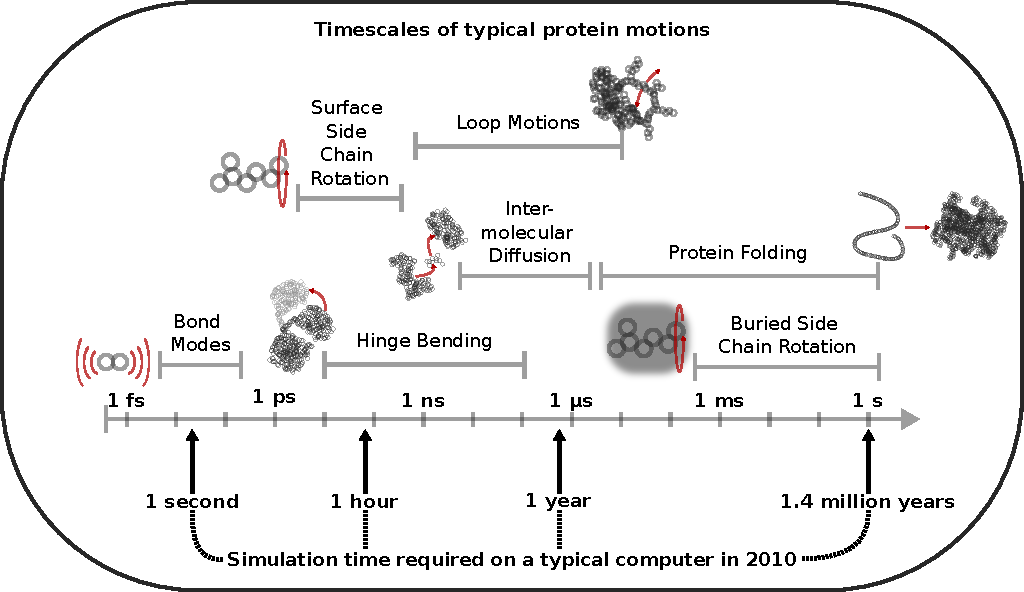
\includegraphics[width=0.48\textwidth]{figures/timescales.pdf}
    \caption{Protein motions occur across a wide range of timescales. Several types of protein motions are illustrated above the time axis with their corresponding time scale. The estimated computational effort required for their simulation is shown below the axis. The wallclock time needed for molecular dynamics simulations for a typical aqueous protein system (~45,000 atoms) varies drastically depending on the protein motion to be studied. The benchmarks were recorded in 2010 with a typical desktop computer. Adapted from Zwier et Chong.\cite{Zwier2010}}
    \label{fig:timescales}
\end{figure}


\subsection{Scope}
Recent advances in computational biophysics and molecular dynamics simulations have led to increasingly sophisticated simulation software. While numerous tutorials exist, they often focus on specialized applications or prioritize practicality over accessibility for beginners. The complexity of MD programs, with their extensive range of options, can overwhelm new users and may exacerbate the choice of simulation conditions and analysis methods. Focus of the present tutorial/training hybrid article is to provide an introduction into MD fundamentals and applications by a series of hands on tutorials that guide through different applications of MD methods. Designed specifically for beginners, the series starts with an essential introduction to the Linux operating system — a prerequisite for installing and using MD simulation software. Through nine carefully structured exercises, users progress from understanding basic MD algorithms to advanced applications, including protein simulations, free energy calculations, and drug design protocols. Each exercise builds upon previous concepts, creating a logical learning progression that bridges the gap between theoretical understanding and practical implementation.\\
\paragraph{Exercise Overview}
\begin{itemize}
    \item \nameref{sec:linuxTut}
    \item \nameref{sec:IntegrationTimestep}
    \item \nameref{sec:ForceField}    
    \item \nameref{sec:tcoupling}
    \item \nameref{sec:TPcoupling}
    \item \nameref{sec:longrangeIA}
    \item \nameref{sec:freeEnerSolv}
    \item \nameref{sec:freeEnerBind}
    \item \nameref{sec:ProteinSim}
    \item \nameref{sec:CompDrugDesign}
\end{itemize}
The tutorial gives the user the essential practical knowledge to set up, run, and analyze MD simulations. Furthermore, this tutorial prompts the user to discuss findings for each exercise in a report and to assess the choice of specific algorithms or parameters. Combined with short discussions in the reports, they add a self-teaching element, furthering understanding and setting this tutorial apart from mere step-by-step tutorials. The tasks can also serve as a basis for developing own setups or design modifications to start own MD simulation endeavors. However, the tutorial is a practical introduction to MD simulation methods, and it does not replace the study of the appropriate literature on theoretical mechanics, statistical mechanics, and thermodynamics to become familiar with the theoretical foundations of MD simulations and analysis of MD data.\\
Each exercise follows a consistent format, beginning with a clear list of tasks accompanied by adequate conceptual artwork that doubles as a visual orientation. The exercises are divided into two main sections: a theoretical foundation and detailed simulation setup instructions. The only exception to this structure is the computational drug design exercise (\fref{sec:CompDrugDesign}), which takes a more application-focused approach, guiding users through various applications important to drug design methodology.\\
The tutorial/training hybrid article is supported by a comprehensive git repository (\githubrepository), structured to facilitate independent learning and classroom instruction. Each exercise has its own directory containing two subdirectories: 'teacher' and 'student.' The 'teacher' directory includes output files, analytical plots, and executable bash scripts that automatically solve the tasks. The lightweight 'student' directory contains only the necessary files for completing the exercise tasks. Additionally, each exercise directory features model reports as reference templates for students to compare their findings. However, these should be considered guidelines rather than definitive solutions since they are genuine student reports. Lecturers interested in using this document as course material are inclined to read the model reports since they are short and represent the net learning outcome.

\newpage

\section{Prerequisites}
A computer with installed Linux OS is preferable, since many installation instructions given herein are tailored to Linux. Nevertheless, an experienced user might as well use any other operating system.


\subsection{Background knowledge}
This tutorial does not require any prior knowledge of the employed programs. However, basic knowledge in molecular biophysics and some knowledge on using computers is recommended. Note, the tutorial is based on a practical course on MD simulations for late stage undergraduates or graduates in biochemistry/physics/computer science or related areas.


\subsection{Software/system requirements}
The leading MD software used in the tutorials is the \texttt{GROMACS} 2018 program. Then, a Python package manager will be required for the last exercise, e.g., \texttt{micromamba}. Compared to the more well-known \texttt{conda} package manager, \texttt{micromamba} is faster, more lightweight, and thus recommended. The installation of \texttt{micromamba} can be postponed until \fref{sec:CompDrugDesign}, where detailed instructions can be found. Visualizing three-dimensional structures is an essential part of molecular sciences, and a suitable program for that purpose is \texttt{VMD}. On their web page, \url{https://www.ks.uiuc.edu/Research/vmd/} installation instructions can be found, which include a quick registration via e-mail. There are other visualization programs, but \texttt{VMD} is recommended since some of the workflows employed in this document assume its availability. Lastly, a program to create scientific plots is required. Program suites like Python or R can be used; however, due to simplicity, the command line tool \texttt{grace} (also known as \texttt{xmgrace}) is recommended. A summary of the requirements and their tested versions is listed below.
\begin{itemize}
    \item \texttt{Ubuntu} 22.04
    \item \texttt{GROMACS} 2018
    \item \texttt{micromamba} 2.0.4 (or a recent version of conda/mamba)
    \item \texttt{VMD} 1.9.3 (recommended)
    \item \texttt{Grace} 5.1 (recommended)
\end{itemize}

\newpage

\section{Exercise 0: Short Introduction to Linux}\label{sec:linuxTut}
\begin{figure}[H]
    \centering
    
\includegraphics[width=0.3\textwidth]{figures/command-line-icon.pdf}
    \caption{This concept art depicts the command line icon. Even though many programs have graphical user interfaces nowadays, a large proportion of scientific software utilizes the command line for speed and flexibility. Image adapted from \url{shmector.com}.}
    \label{fig:Commandline-icon}
\end{figure}


\subsection*{Tutorial on Linux/BASH (optional)}
GNU/Linux is a UNIX-type operating system. It is free software, thus free of charge, and the source code can be downloaded and changed to fit individual needs. Several different distributions are available and many distributions offer a graphical user interface similar to Windows or MacOS. However, in the Linux world, utilizing a text-based interface (the shell) is standard, usually running in a terminal window. The shell reads and interprets user commands. After pressing enter, the commands are executed, and the output, if any, is displayed on the screen (\texttt{STDOUT}). In this section, a few features are introduced, offered by the Bourne-again shell (\texttt{Bash}), the most common shell in the Linux world. Many excellent online introductions exist for using the Unix/Linux operating system.\\
On \url{webminal.org/login/}, a terminal emulator can be found, i.e., a virtual terminal where Unix/Linux commands can be executed only via an e-mail registration. It also contains a tutorial section. Another terminal emulator that does not require registration but does not offer a tutorial can be found at \url{bellard.org/jslinux/}. The "UNIX Tutorial for Beginners" by Michael Stonebank at the University of Surrey can be done online (\url{www.ee.surrey.ac.uk/Teaching/Unix}). An extensive tutorial on Linux is provided by the "Cornell Virtual Workshop" (\url{www.cac.cornell.edu/VW/Linux}). 


\subsection*{Basic Commands}
The user must first open a terminal window to use the command prompt. On most Linux systems, this can be done by using the keyboard shortcut \keystroke{Ctrl} + \keystroke{Alt} + \keystroke{T}. Some of the most useful commands are listed below. Beginners should execute some of them in the terminal. Start with the easier ones, such as \code{ls}, \code{cd}, and \code{echo}.
\begin{description}
	\item[\code{awk}]\hfill \\
	 While the other entries in this list are mostly programming tools, \code{awk} is a \textit{Turing complete} programming language specifically designed to alter files. Some utilities might be helpful for this course. 
	 
	 \item[\code{cat} \texttt{<file>}]\hfill \\ 
	 The content of \texttt{<file>} is printed to \texttt{STDOUT}. It can also be redirected into another file (\code{>}) or be used as an input for a follow-up command (\code{|}).
	 
	 \item[\code{cd} \texttt{<dir>}]\hfill \\ 
	 Change the directory to \texttt{<dir>}. \code{cd} changes to the home directory without an input option.
	 
	 \item[\code{chmod} \texttt{<octalnum>} \texttt{<file>}]\hfill \\ 
	 Modifies the user permissions of \texttt{<file>} according to 
	 \texttt{<octalnum>}. \code{chmod} is necessary to make files executable.
	 
	 \item[\code{cp} \texttt{<file> <filename>}]\hfill \\ 
	 Copies \texttt{<file>} to another file called \texttt{<filename>}. Linux assumes the users know what they are doing and overwrites any other file with the same name without question.
	 
	 \item[\code{echo} \texttt{<string>}]\hfill \\
	 Takes \texttt{<string>} as an input text and prints it to \texttt{STDOUT}. It can also be redirected into another file (\code{>}) or be used as an input for a follow-up command (\code{|}).
	 
	 \item[\code{grep} \texttt{<pattern> <input>}]\hfill \\ 
	 Search the \texttt{<input>}, which can be a file or a text, for the \texttt{<pattern>} and print the matching lines to \texttt{STDOUT}. The pattern can be a so-called \textit{regular expression} (\texttt{REGEX}) or a simple text string.
	 
	 \item[\code{history}]\hfill \\
	 This command prints a handy command history for keeping track or as a look-up if commands should be concatenated into an automatic script.
	 
	 \item[\code{htop}]\hfill \\ 
	 Opens the interactive process viewer, which compares to the Windows task manager. CPU and memory usage, as well as all processes, can be monitored. Also, it makes the user feel like a hacker. Press \keystroke{q} to exit back to the shell.
	 
	 \item[\code{locate} \texttt{<pattern>}]\hfill \\ 
	 Locates files that match \texttt{<pattern>}. The pattern can either be a \texttt{REGEX} or any text string that is part of the file you seek.
	 
	 \item[\code{ls} \texttt{<path>}]\hfill \\ 
	 List the contents of \texttt{<path>} to \texttt{STDOUT}. Note that \texttt{<path>} can also refer to any directory or a group of files. \code{ls} can also be prompted without \texttt{<path>} to list the current directory. \code{ls} offers many options and is probably the most used command for Linux users. 
	 
	 \item[\code{man} \texttt{<executable>}]\hfill \\ 
	 The command's manual is opened, showing detailed information about the command given in \texttt{<executable>}. Tap \keystroke{q} to leave the man page.
	 
	 \item[\code{mkdir} \texttt{<dirname>}]\hfill \\ 
	 Create a directory called \texttt{<dirname>} in the current directory.
	 
	 \item[\code{mv} \texttt{<file> <filename>}]\hfill \\ 
	 Like \code{cp}, but the original \texttt{<file>} is removed in the process. Use with caution. If \texttt{<filename>} corresponds to a directory, the file is moved into that directory.
	 
	 \item[\code{pwd}]\hfill \\ 
	 prints the current directory path to \texttt{STDOUT}.
	 
	 \item[\code{rm} \texttt{<file>}]\hfill \\ 
	 This command removes \texttt{<file>} from the disk. Therefore, \texttt{<file>} is not moved to the bin like in Windows but deleted beyond recovery.
	 
	 \item[\code{rmdir} \texttt{<dir>}]\hfill \\ 
	 Remove an empty directory \texttt{<dir>}.

	\item[\code{sed} \texttt{<option>} \texttt{<file>}]\hfill \\ 
	 \code{sed} is a \textit{turing complete} tool originally used for text filtering and manipulation and offers diverse automatic applications in this field. Mostly, this command is used to delete, insert, and substitute text in files exactly where the user wants it.
	 
	 \item[\code{sort} \texttt{<input>}]\hfill \\ 
	 \texttt{<input>}, either a file or text string, is sorted alphabetically. Often, this command receives its input via the pipe \code{|}.
	 
	 \item[\code{tail} \texttt{<N> <file>}]\hfill \\ 
	 The \texttt{<N>} last lines of \texttt{<file>} are printed to \texttt{STDOUT}. It can also be redirected into another file (\code{>}) or be used as an input for a follow-up command (\code{|}).
	 
	 \item[\code{vim} \texttt{<file>}]\hfill \\ 
	 the \texttt{VIM} editor opens a file for editing. A steep learning curve accompanies its usage.
	 
	 \item[\code{wc} \texttt{<input>}]\hfill \\ 
	 This command means \textit{word count}; thus, it counts words in the given input. Furthermore, if given the appropriate options, it counts lines, characters, and bytes.
	 
	 \item[\code{whoami}]\hfill \\
	 prints the current user to \texttt{STDOUT}.
\end{description}
Remember that these commands can change their behavior when particular options are specified. For Linux commands, these options are usually specified by '\code{-}' followed by the \texttt{flag}, e.g., \code{ls} list the directory content. However, \code{ls -l} lists the contents more verbosely and gives information about permissions, disk usage, and the latest access. Another example would be \code{mv file file2}, which renames \texttt{file} to \text{file2} without communicating to the user. If \code{mv -v file file2} is specified, on the other hand, the command is more verbose and prints information to \texttt{STDOUT}. Most commands reveal the available options by specifying \code{-{}-help}, e.g., \code{sort -{}-help}.


\subsection*{Managing Files and Directories}
Try to find out how to use the following commands, i.e., what inputs to use after each command in order to make them work:
\begin{lstlisting}[language=bash]
# comments start with '#'; they will not be executed by bash
mkdir # create new, empty directory
touch # create new, empty file
cp    # copy one or multiple files
cp -r # recursively copy one directory and its content to another one
rmdir # remove one empty directory
rm    # remove one or multiple files
\end{lstlisting}
Use \code{man} or specify \code{-{}-help} when in doubt. \code{rm} and \code{cp} aswell as most other linux commands allow for something called \textit{globbing}. Globbing does not require a comprehensive file name. Instead, an expression suffices resembling a variety of file names that match the so-called \texttt{glob}, e.g., use the wildcard \code{*} to match any pattern in the file name. For instance, \code{rm *.txt} will delete any file with the \texttt{.txt} extension. The question mark wildcard \code{?} represents exactly one character, which can be any single character. Two question marks in succession would represent any two characters in succession, and three question marks in succession would represent any string consisting of three characters. For instance, \code{rm ???} will delete any file whose name contains exactly three characters (including the extension). \code{rm ???.txt} will delete any file with the .txt extension whose name contains exactly three characters. Both, \code{?} and \code{*} can be combined.\\
The \code{mv} command renames a file. The second input argument can either be a file, an absolute path, or a relative path, which holds for \code{cp} and \code{rm}.
\begin{lstlisting}[language=bash]
mv file1 file2    # If file2 exists it will be overwritten
mv file1 dir1     # moves file1 to a directory called dir1
mv dir1/file1 ../ # move file1 from directory1 to parent folder (../)
\end{lstlisting}


\subsection*{VIM/VI}
One of the popular UNIX editors is \texttt{vi} (or \texttt{VIM}), which stands for visual editor. \texttt{vi} is a full-screen editor and has two main modes of operation:
\begin{itemize}
	\item Command mode: commands to specify an action on the file.
	\item Insert mode: where text is inserted into the file.
\end{itemize}
In the Command mode, every character typed is a command that does something to the edited text file. Take into account that both UNIX and vi are case-sensitive. Thus, the action performed on a file when typing y will not be the same as when typing Y.
\code{vi <filename>} creates a new file. If the file already exists, the first lines will be shown on the screen, similar to other text editors. The following commands can be used to save and exit the file:
\begin{lstlisting}[language=bash]
:q  # quit vi without saving. This command will only work for unmodified files
:q! # quit vi without saving the last changes
:w  # save (write) the file
:wq # save (write) the file and quit vi
:x  # save and quit the file (exactly as :wq)
:w new_filename   # save the current file with a different name
:wq new_filename  # save the current file with a different name and exit. This command will only work if new_filename is not the name of any existing file in the current directory
:wq! new_filename # save the current file with a different name and exit; overwrites existing file with the name new_filename
\end{lstlisting}
To switch to the \texttt{insert mode}, either \code{i}, \code{I}, \code{a}, \code{A}, \code{o} or \code{O} can be used. See below for the meaning of each specific command. Once in the \texttt{insert mode}, every character typed is added to the text in the file. To turn off the insert mode, \keystroke{Esc} can be used.
\begin{lstlisting}[language=bash]
i # insert text before cursor
I # insert text at beginning of current line
a # append text after cursor
A # append text to end of current line
o # insert text in a new line below current line
O # insert text in a new line above current line
\end{lstlisting}
Furthermore, there is a \texttt{replace mode} accessible by hitting \keystroke{shift}+\keystroke{R}. Switching between the \texttt{insert mode} and the \texttt{replace mode} is also possible by pressing \keystroke{Insrt}. More specific options exist to modify file contents via \texttt{VIM}. Only some of them are listed below.
\begin{lstlisting}[language=bash]
r # replace single character under cursor
x # delete single character under cursor
Nx # delete N characters, beginning with current character
dw # delete single word, beginning with current character
C # change characters in the current line
D # delete remainder of the current line
Y # copy remainder of the current line
cw # change the current word with new text
cc # change entire current line
dd # delete entire current line
yy # copy entire current line
cNw # change the next N words, beginning with the current
cNc # change the next N lines, beginning with the current
dNw # delete the next N words, beginning with the current
dNd # delete the next N lines, beginning with the current
yNy # copy the next N lines, beginning with the current
p # paste the previously copied/deleted lines/words after the current line
\end{lstlisting}
Undoubtedly, two of the most important commands are redo/undo, which are available in \texttt{VIM} by typing \keystroke{u} for undoing and \keystroke{Ctrl}+\keystroke{r} for redoing. At this point, \texttt{VIM} can be used just like any other text editor. However, it is much more versatile. It can search the text for text patterns and replace them with new text using convenient shortcuts. Some of those shortcuts are listed below. Furthermore, \texttt{VIM} has numerous plug-ins since it is open source with a lively community, e.g., you could run latex by just using \texttt{VIM}.
\begin{lstlisting}[language=bash]
/word # search forward for the pattern 'word' in text.
?word # search backward for the pattern word in text
n # move to following occurrence of search string
N # move to preceeding occurrence of search string
gg # go to the first line
G # go to the last line
:%s/pattern1/pattern2/g # replace word pattern1 by pattern2 throughout the whole file
\end{lstlisting}
For a more hands-on introduction to \texttt{VIM}, you may use \code{vimtutor}. This program gets installed simultaneously with \texttt{VIM} and can be opened by typing \code{vimtutor} in your command line. It contains seven interactive lessons, teaching the very basics of the program.

\newpage

\section{Exercise 1: Energy Conservation and Integration Algorithms}\label{sec:IntegrationTimestep}
% Here is a single-column checklist that consists of multiple sub-checklists
\begin{Checklists}
    \begin{checklist}{Tasks for the First Exercise}
    \textbf{Finish these tasks and write a short report about your findings.}
    \begin{itemize}
    		\item Include plots containing $E_\text{kin}$, $E_\text{pot}$ and $E_\text{tot}$ for each of the 12 simulations you have to conduct: one correctly propagated simulation, one simulation that fails to conserve $E_\text{tot}$ and one simulation that 'explodes'.
    		
    		\item Briefly explain your results and state what time step you would choose for the respective system to conserve energy but still simulate as long as possible. How can you explain the correlation between particle mass and choice for the time step?
    \end{itemize}
    \end{checklist}
\end{Checklists}
\begin{figure}[H]
    \centering
    
\includegraphics[width=0.48\textwidth]{figures/ComputationalBioPhysicsConcept.png}
    \caption{A computer screen showing an elusive protein structure to welcome the reader to computational biophysics. Art created with DALL-E.}
    \label{fig:ComputationalBioPhysicsConcept}
\end{figure}


\subsection*{Introduction to \texttt{GROMACS} }
% Gromacs description and introduction to time step
\texttt{GROMACS}\cite{Abraham2015,Hess2008} is a highly optimized open-source software for molecular dynamics (MD) simulations of biomolecules like proteins, DNA, and lipids. A basic task of this command-line program is to integrate Newton's equations of motion to generate a time series, also known as a trajectory, of a given molecular system. The tutorial introduces first the workflow and the fundamentals of \texttt{GROMACS}. It will then focus on the choice of the integration time step, which is one of the most fundamental parameters of an MD simulation. Its importance originates from the limitations of computational resources. \\
% Real Time triangle
The computational resources, hence the available hardware, determine the quality of three interdependent constraints, the most important one being the real-time needed to complete the simulation. The other two constraints are the system size (number of equations) and simulation time (number of times said equations are solved). The system size usually depends on the scientific problem at hand. Therefore, the simulation time is the most flexible of the three constraints that can also be modulated by the integration time step (see \fref{fig:tt}).
%%% can be two separate pictures
\begin{figure}
	\begin{subfigure}[c]{0.25\textwidth}
		\centering
		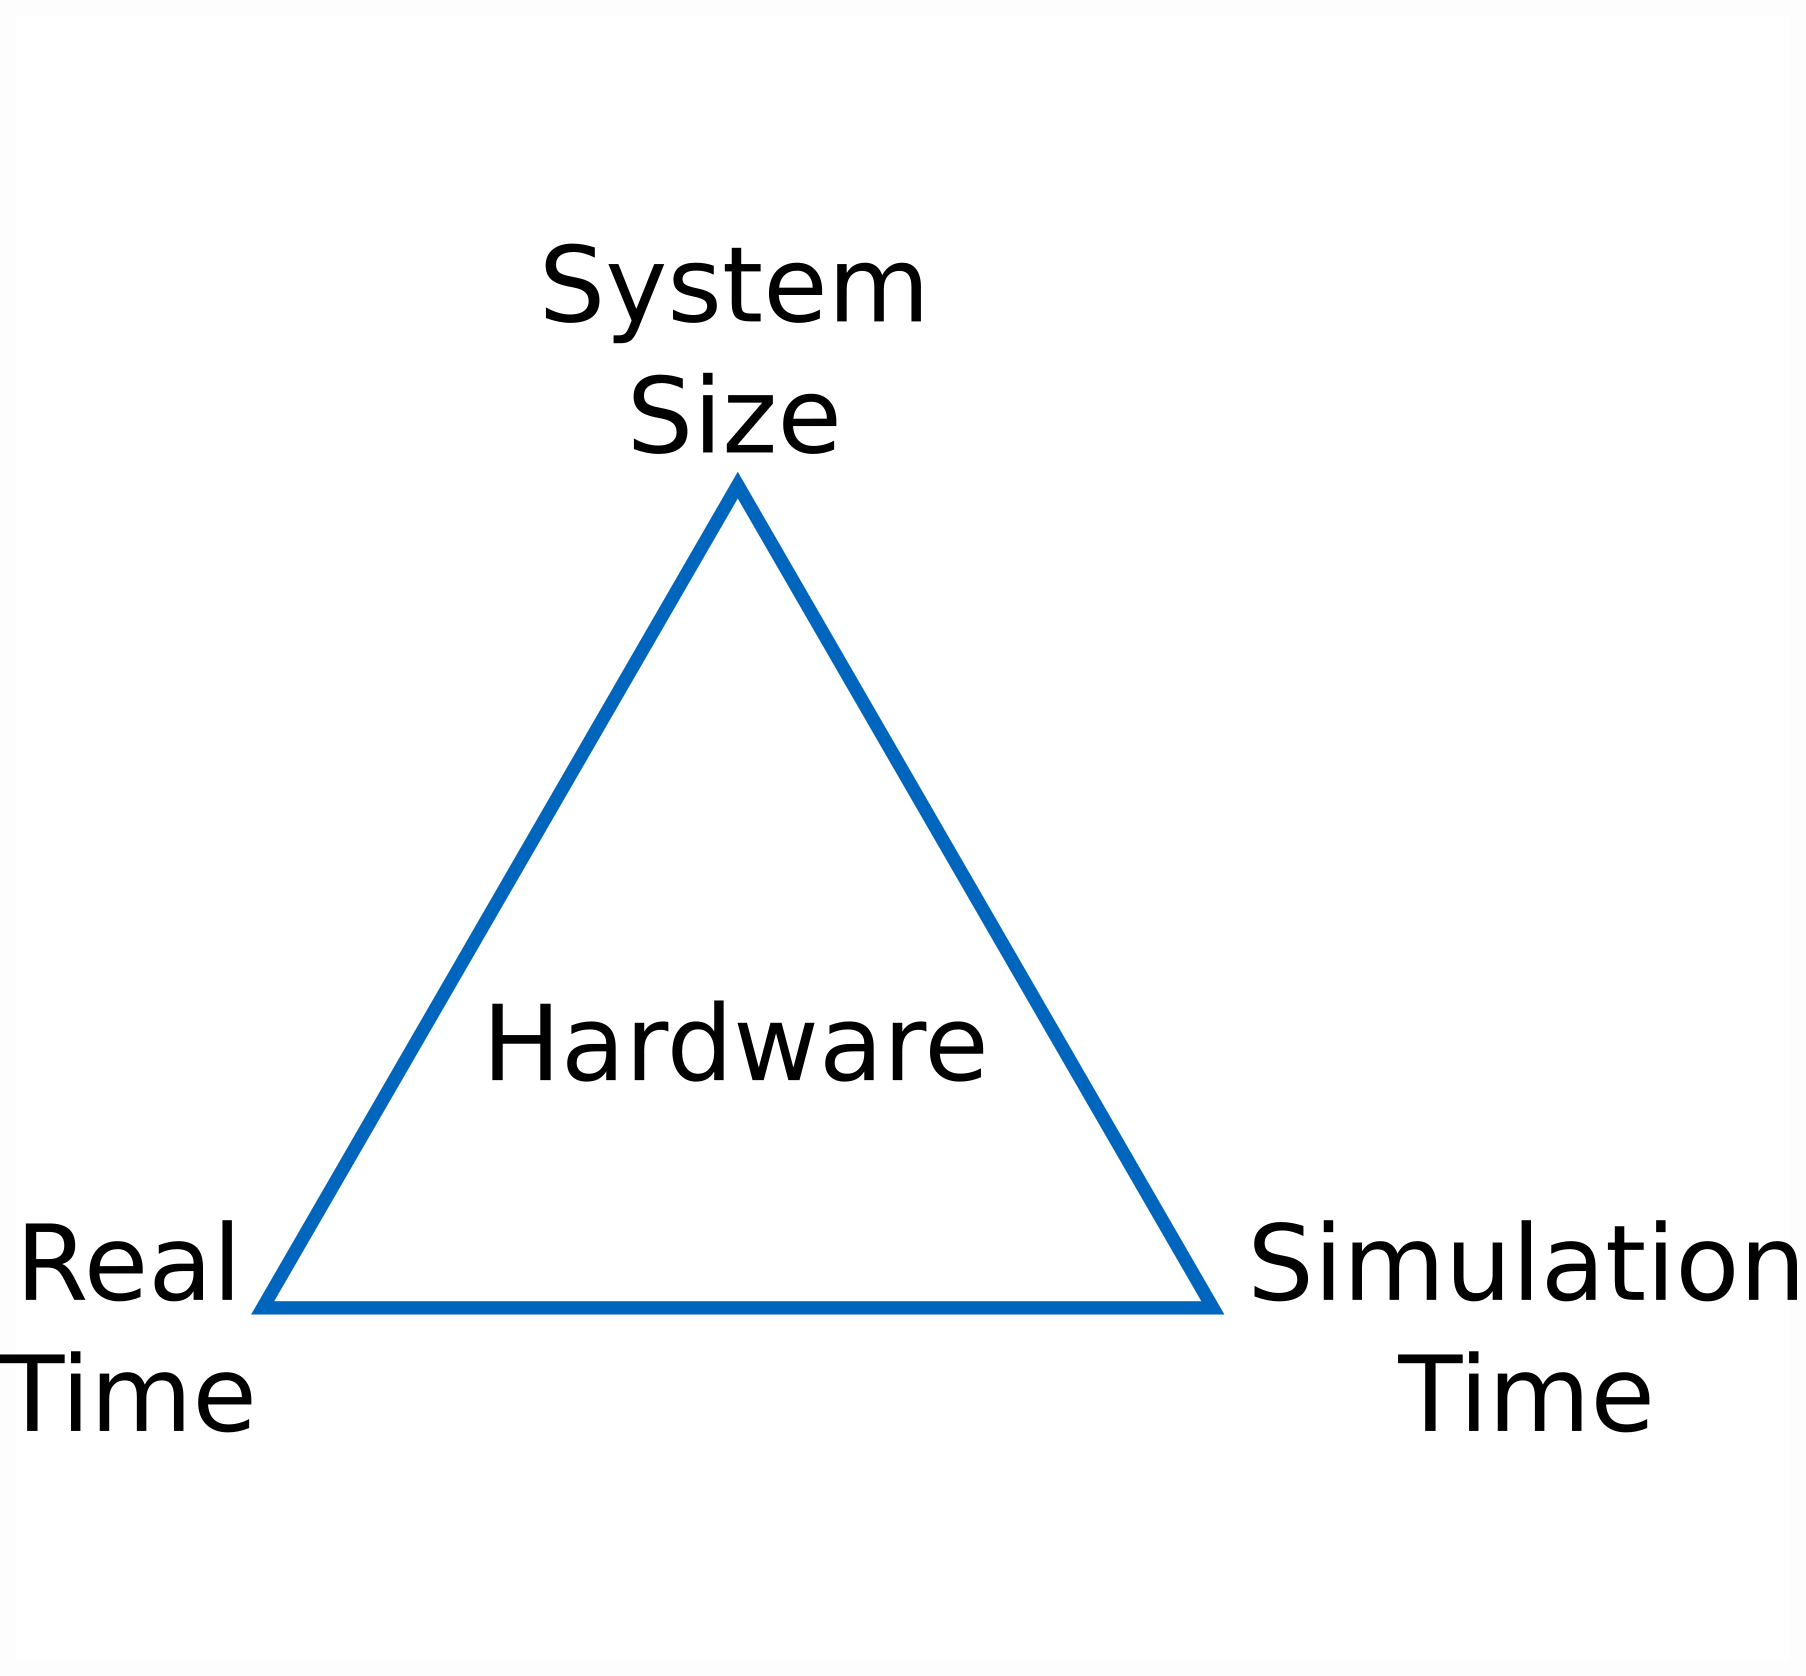
\includegraphics[width=0.8\textwidth]{figures/tradeoffTriangle.png}
		\caption{For a given hardware, the user must trade between real-time, simulation time, and the system size. The system size or the simulation time must be sacrificed for less real-time passing during the simulation.}
		\label{fig:tt}
	\end{subfigure}
	~
	\begin{subfigure}[c]{0.25\textwidth}
		\centering
		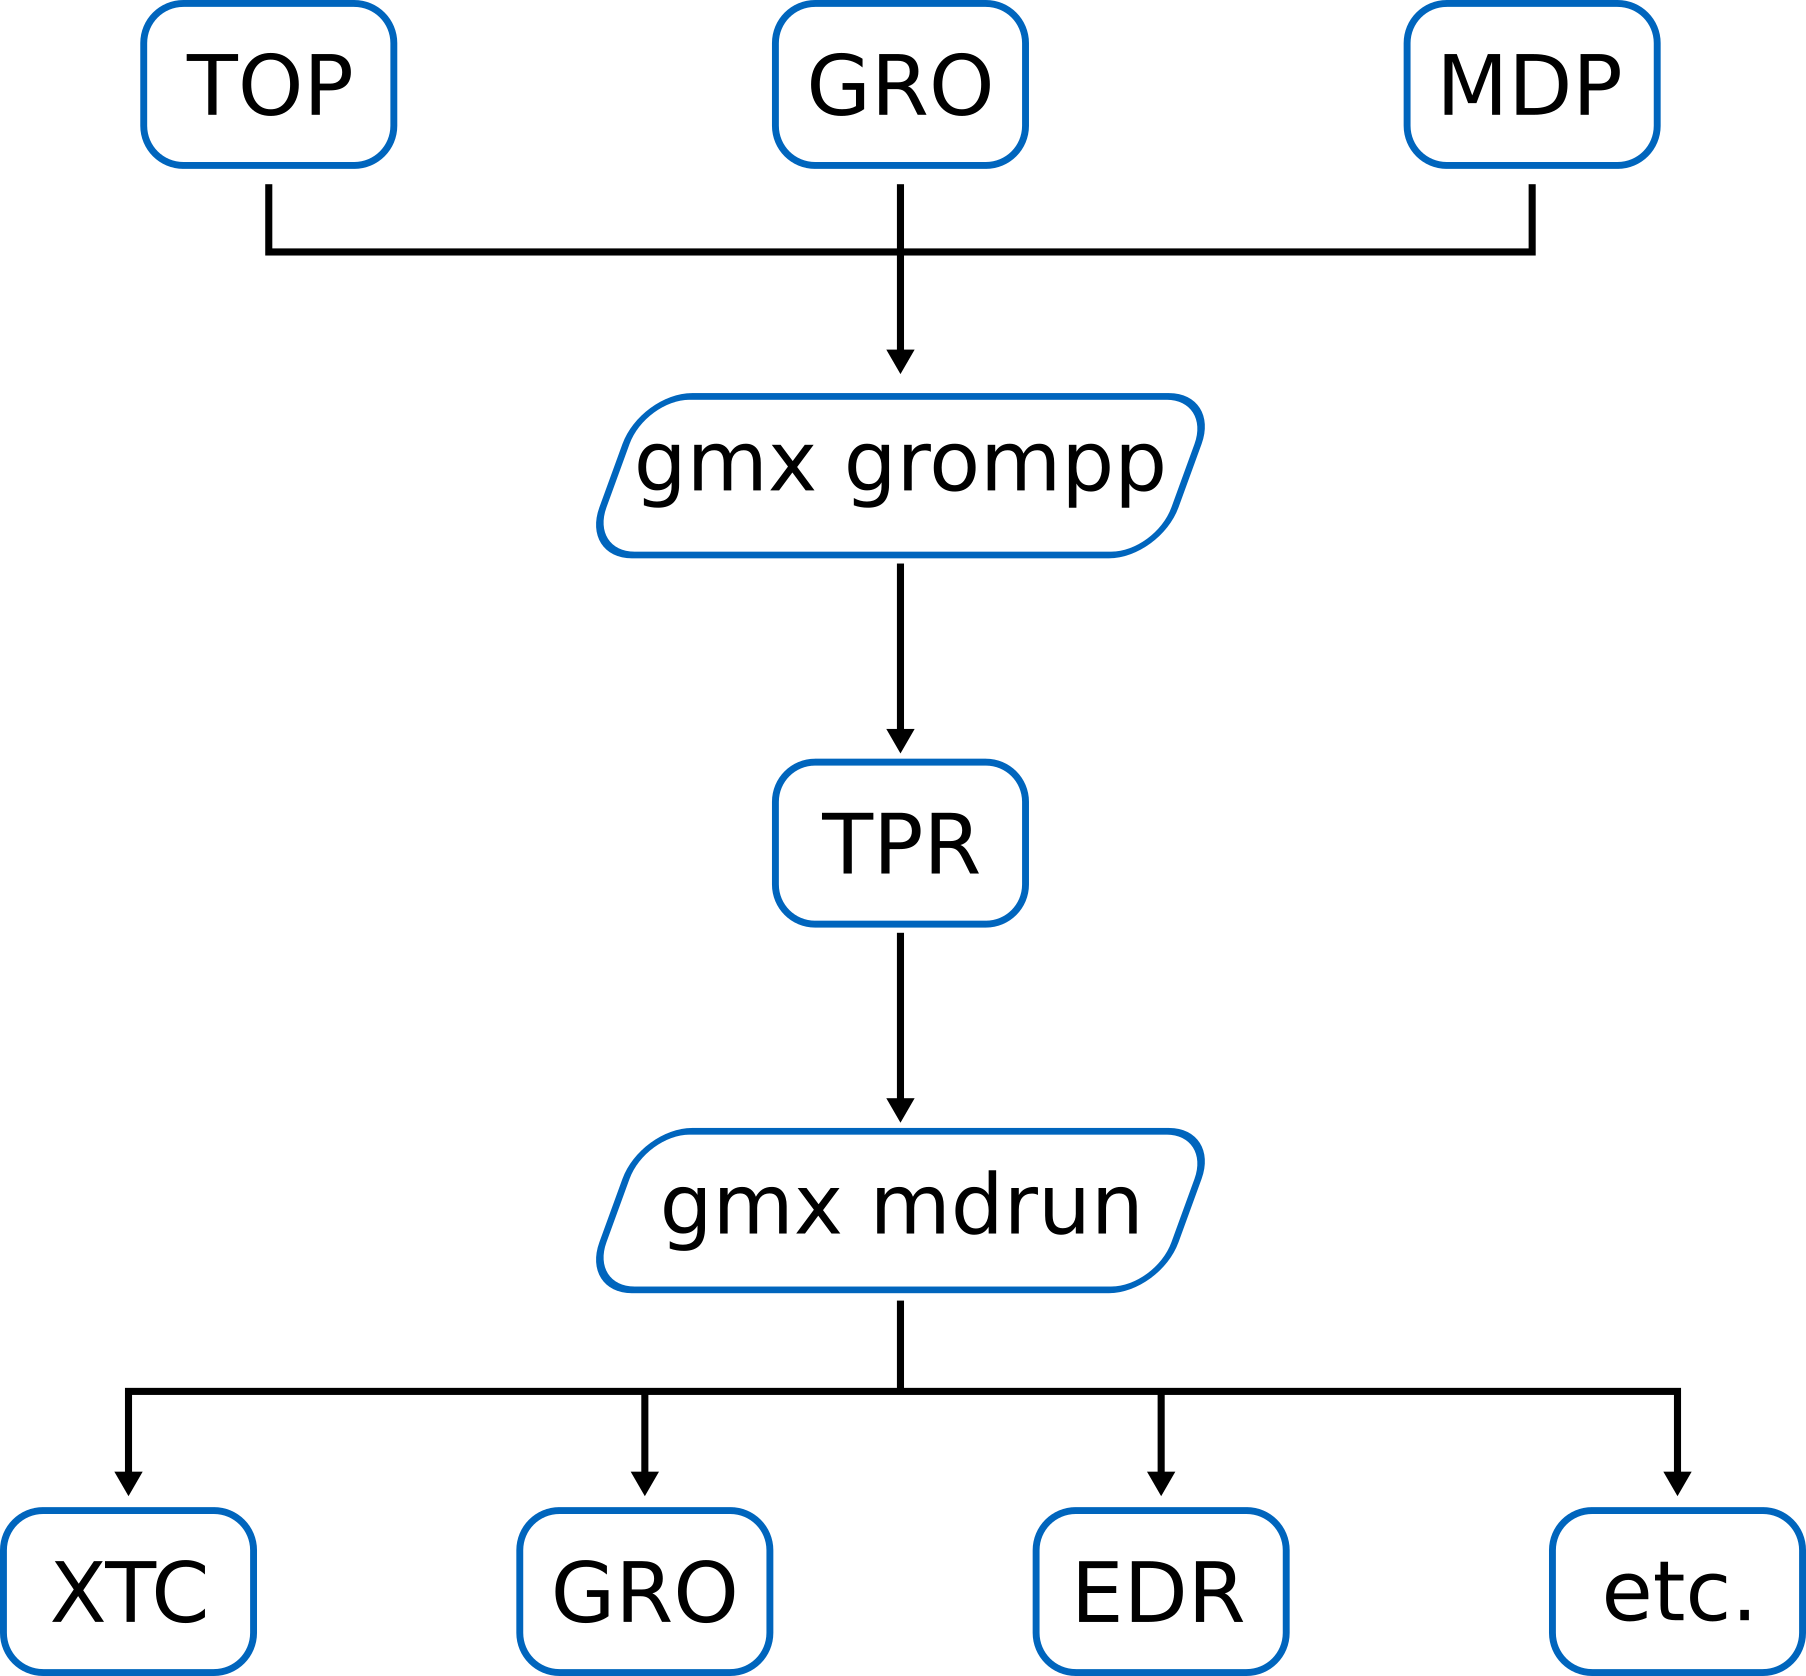
\includegraphics[width=0.8\textwidth]{figures/gromacsworkflow.png}
		\caption{The workflow in \texttt{GROMACS} uses the commands \code{gmx grompp} and \code{gmx mdrun} to generate diverse output files from three standardized input files.}
		\label{fig:gmxwf}
	\end{subfigure}
\end{figure}\noindent


\subsection*{Theoretical Considerations}
The integration time step is related to how Newton's equations of motion are solved in the computational framework. Assuming, $N$ particles the motions governing particle movement are dependent on the forces $F$ on each particle and the potential energy function $U_\text{\tiny tot}$ which depends on the configuration of all particles $\Vec{r}^N = \{r_0,...,r_i,..,r_N\}$.\cite{Allen1990} The potential energy function is also called the forcefield and presents the cardinal assumption underlying every MD simulation. It will be elaborated on in \fref{sec:ForceField}.
\begin{align}\label{eq:NewtonsEqOfMotion}
    F(r_i) & = -\frac{\partial U_\text{\tiny tot}}{\partial r_i} \\
    F(r_i) & = m_i\frac{d^2 r_i}{dt^2}
\end{align}
Solving these equations analytically for more than two particles is not possible, and therefore numerical algorithms have been developed all of which rely on the user's choice of the integration time step. One of the simpler implementations is the Euler method that iteratively applies the following two equations to generate molecular configurations $\Vec{r}^N$ which are then used to calculate the forces in \fref{eq:NewtonsEqOfMotion}.\cite{Atkinson1989}
\begin{align}
    r_i(t + \Delta t) &= r_i(t) + v_i(t)\Delta t \\
    v_i(t + \Delta t) &= v_i(t) + \frac{F_i(t)}{m_i}\Delta t
\end{align}
It can be shown, that the error resulting from this method is in the order of $\Delta t$.\cite{Iserles2008_page8} Other algorithms like the verlet algorithm and the leap-frog algorithm (a variation of the verlet algorithm\cite{Allen1990}) generate truncation errors that are in the order of $\Delta t^4$ which presents a substantial improvement.\cite{Kim2014} The leapfrog integrator is the default setting that \texttt{GROMACS} applies and it uses the half-step velocities to generate the coordinates of the next step.\cite{Allen1990}
\begin{align}
    r(t + \Delta t) & = r(t) + \Delta t \cdot v(t+\tfrac{1}{2}\Delta t)\\
    v(t + \tfrac{1}{2} \Delta t) &= v(t - \tfrac{1}{2} \Delta t) + \Delta t \cdot a(t)
\end{align}
%%% TODO Show that leap frog and verlet are algebraically identical as stated in allen1990 p 81
Another benefit of the leapfrog integrator is its time-reversibility which ensures the conservation of energy.\cite{Kim_2014}. Apart of truncation errors, other error sources include round-off errors and errors from improper sampling of the fastest movement within the molecular system. Thus, the following question emerges: How large can the time step be without destabilizing the system? Small-time steps cannot capture biological processes within reasonable real-time, and steps that are too large lead to truncation errors in the integration algorithm thereby violating energy conservation.


\subsection*{Setup and Simulations}
% Aim: getting to know GROMACS and limits of the integrator
This exercise aims to get accustomed to \texttt{GROMACS} and understand the stability of time integration algorithms and their dependency on particle mass. Herein, four systems should be simulated with different time steps. For each system, the different time steps should generate a correct trajectory, one trajectory where the energy conservation is violated, and one with a time step unreasonably high so that the simulation becomes numerically unstable resulting in chaotic motion not conserving energy and other physical quantities. 


\subsubsection*{GROMACS Workflow}
Unlike many everyday programs, \texttt{GROMACS} does not have a graphical user interface due to its manifold functionalities. Instead, it executes commands and tools via the command line. E.g., a very simple command is \code{gmx -{}-version} which outputs version information about \texttt{GROMACS} onto the screen.\\
\texttt{GROMACS} requires three different files to run a simulation: \texttt{TOP}-, \texttt{MDP}- and \texttt{GRO}-file. Each file contributes different information to \texttt{GROMACS}. The \texttt{GRO}-file contributes the atomic positions and velocities, the \texttt{TOP}-file contributes the information about the atomic and molecular attributes (the topology), and the \texttt{MDP}-file is short for the molecular dynamics parameters, and determines which algorithms to use and how to tune them. The command \code{gmx grompp} takes these three files as input with their respective flags and outputs the \texttt{TPR} file that can be subsequently used to start the MD run via \code{gmx mdrun} (see \fref{fig:gmxwf}). In a nutshell, \code{gmx grompp} is the MD run preparation tool, and \code{gmx mdrun} calls the simulation engine. A variety of output files are generated by \code{gmx mdrun}, which are explained in the \texttt{GROMACS} command line reference (see \url{manual.gromacs.org/documentation/2018/onlinehelp/gmx-mdrun.html} for further information). 
\begin{table}[H]
    \centering
    \caption{\texttt{GROMACS} file formats specified by their suffices with a concise description. This table is not comprehensive. Further information are available on the \texttt{GROMACS} webpage.}
    \label{tab:gromacsFileDesc}
    \begin{tabular}{r p{7cm}}
        \toprule
        Suffix & Short Description \\
        \midrule
        .tpr & \texttt{GROMACS} binary run input file, contains simulation parameters and is generated via \code{grompp} \\
        .gro & Coordinate file in \texttt{GROMACS} format. Contains positions, velocities and box dimensions. \\
        .top & Topology file defining molecular structure such as molecules, bonds and types of interactions.\\
        .mdp & \texttt{GROMACS} parameter file, contains simulation settings, like the time step, run time and thermodynamic ensemble.\\
        .trr & Compressed binary trajectory file containing positions and velocities of all particles over the course of the simulation. \\
        .xtc & Compressed binary trajectory file in \texttt{XTC} format. \\
        .edr & Binary energy file, contains simulation energy data for analysis by \texttt{GROMACS} command line tools, e.g. \code{gmx energy}.\\
        .log & Humand-readable log file with detailed simulation output.\\
    \bottomrule
    \end{tabular}
\end{table}

The most important for today's tutorial is the \texttt{EDR} file outputted by \code{gmx mdrun}. In this file, the energetic information about the system is saved, which can be analyzed via \code{gmx energy} to extract specific information and plots. \code{gmx energy} is an interactive command that selects the energetic properties for information collection. The interface is terminal-based and typically looks like shown in \fref{fig:gmxenergyIA}. Selecting the energetic properties within the interface is conducted by typing the corresponding number followed by hitting \keystroke{Enter} twice, e.g., for the kinetic energy in \fref{fig:gmxenergyIA}, type \keystroke{5}~+~\keystroke{Enter}~+~\keystroke{Enter}.
\begin{figure}
    \centering
    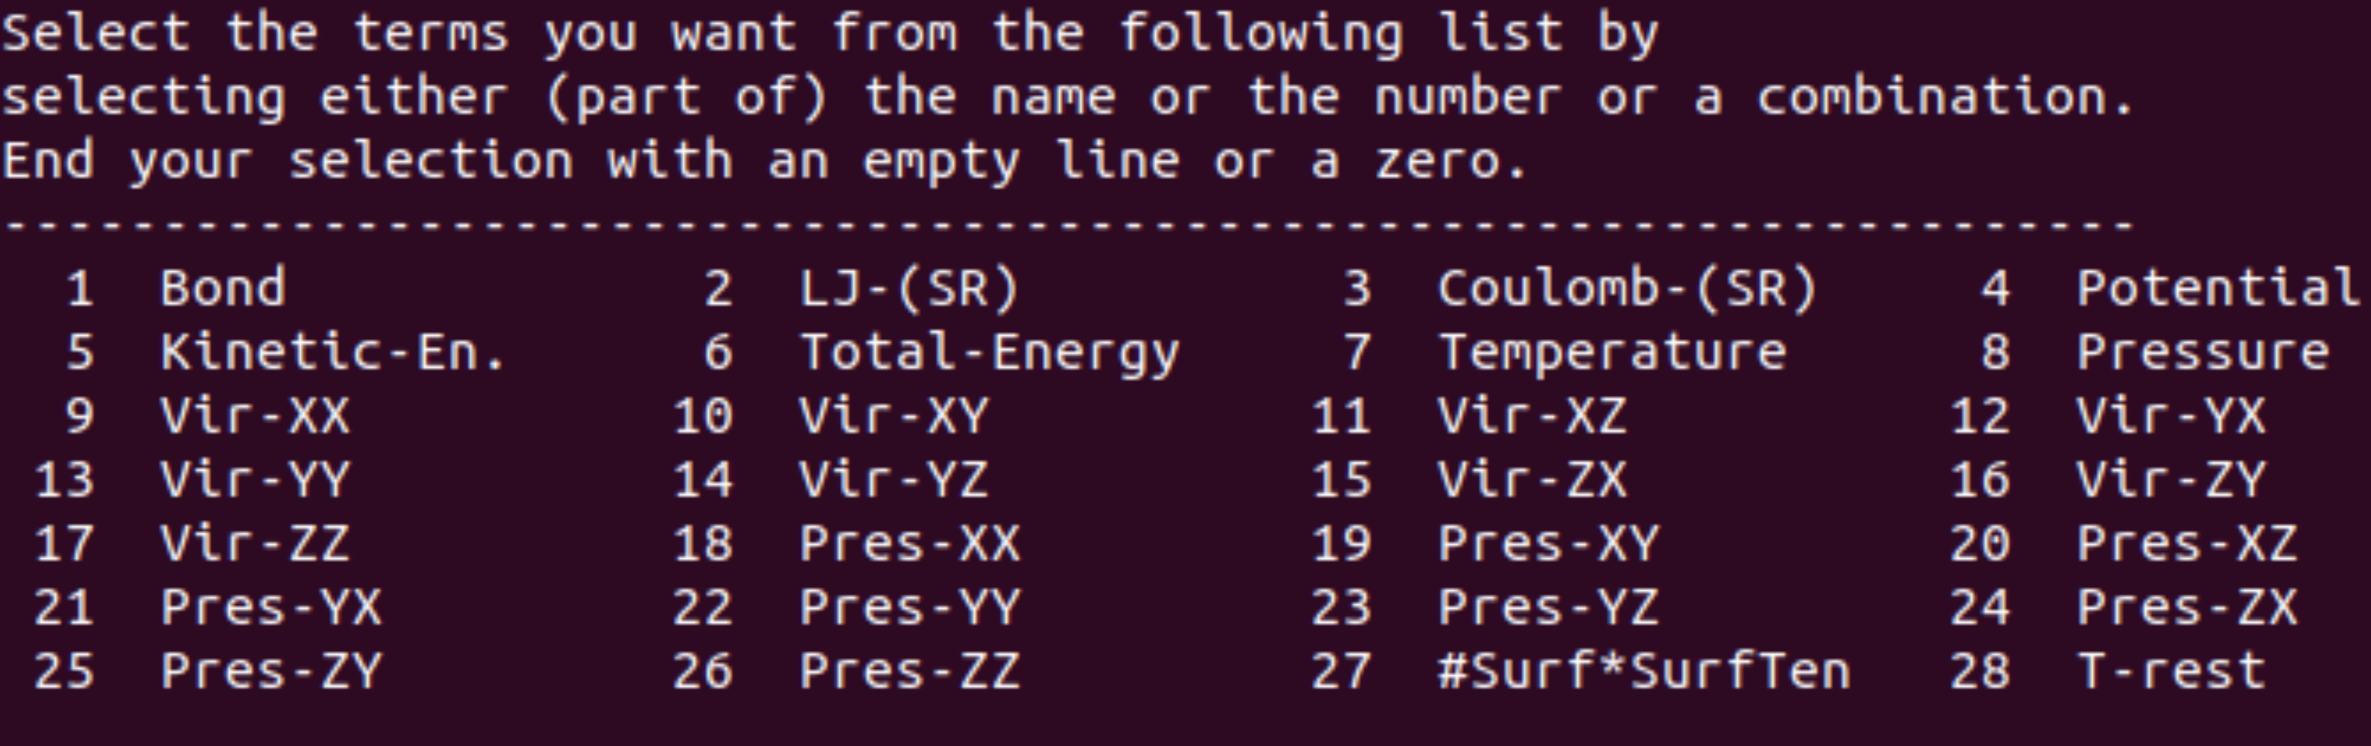
\includegraphics[width=0.48\textwidth]{figures/energyIA.png}
    \caption{User interaction after executing \code{gmx energy}. Multiple options can be selected at once by typing the number or the whole name of the energetic term.}
    \label{fig:gmxenergyIA}
\end{figure}\noindent
The user interaction can be skipped by pre-defining the terms of interest with \code{printf} and \code{|}. The vertical line is called a pipe and can chain different commands. \code{\textbackslash n} is code for a newline and is equivalent to \keystroke{Enter} for the user interaction.
\begin{lstlisting}[language=bash]
printf "4\n5\n6\n" | gmx energy -f <...>.edr -o <...>.xvg
\end{lstlisting}
Conclusively, the workflow for one system in this tutorial consists of the input file preparation (\code{grompp}), the actual simulations (\code{mdrun}), and the analysis of the energetic contributions (\code{energy}). 


\subsubsection*{Effect of Time Step on the Stability of MD Simulations with GROMACS}
Four different systems are used in this tutorial and are represented by the corresponding input files stored in the online repository. The coordinate file \code{intro.gro} represents a box of diatomic particles that should be used for all simulations. The topologies \code{topol\_*.top} differ concerning the particle mass and the parameter file \code{intro.mdp} contains no value for the \code{dt} option, i.e., the simulation time step. This vacancy is deliberate since the main task for the user is to tinker with this option (further elaborated later on in this section). A detailed understanding of the input files is not necessary at this stage.
\begin{figure}
    \centering
    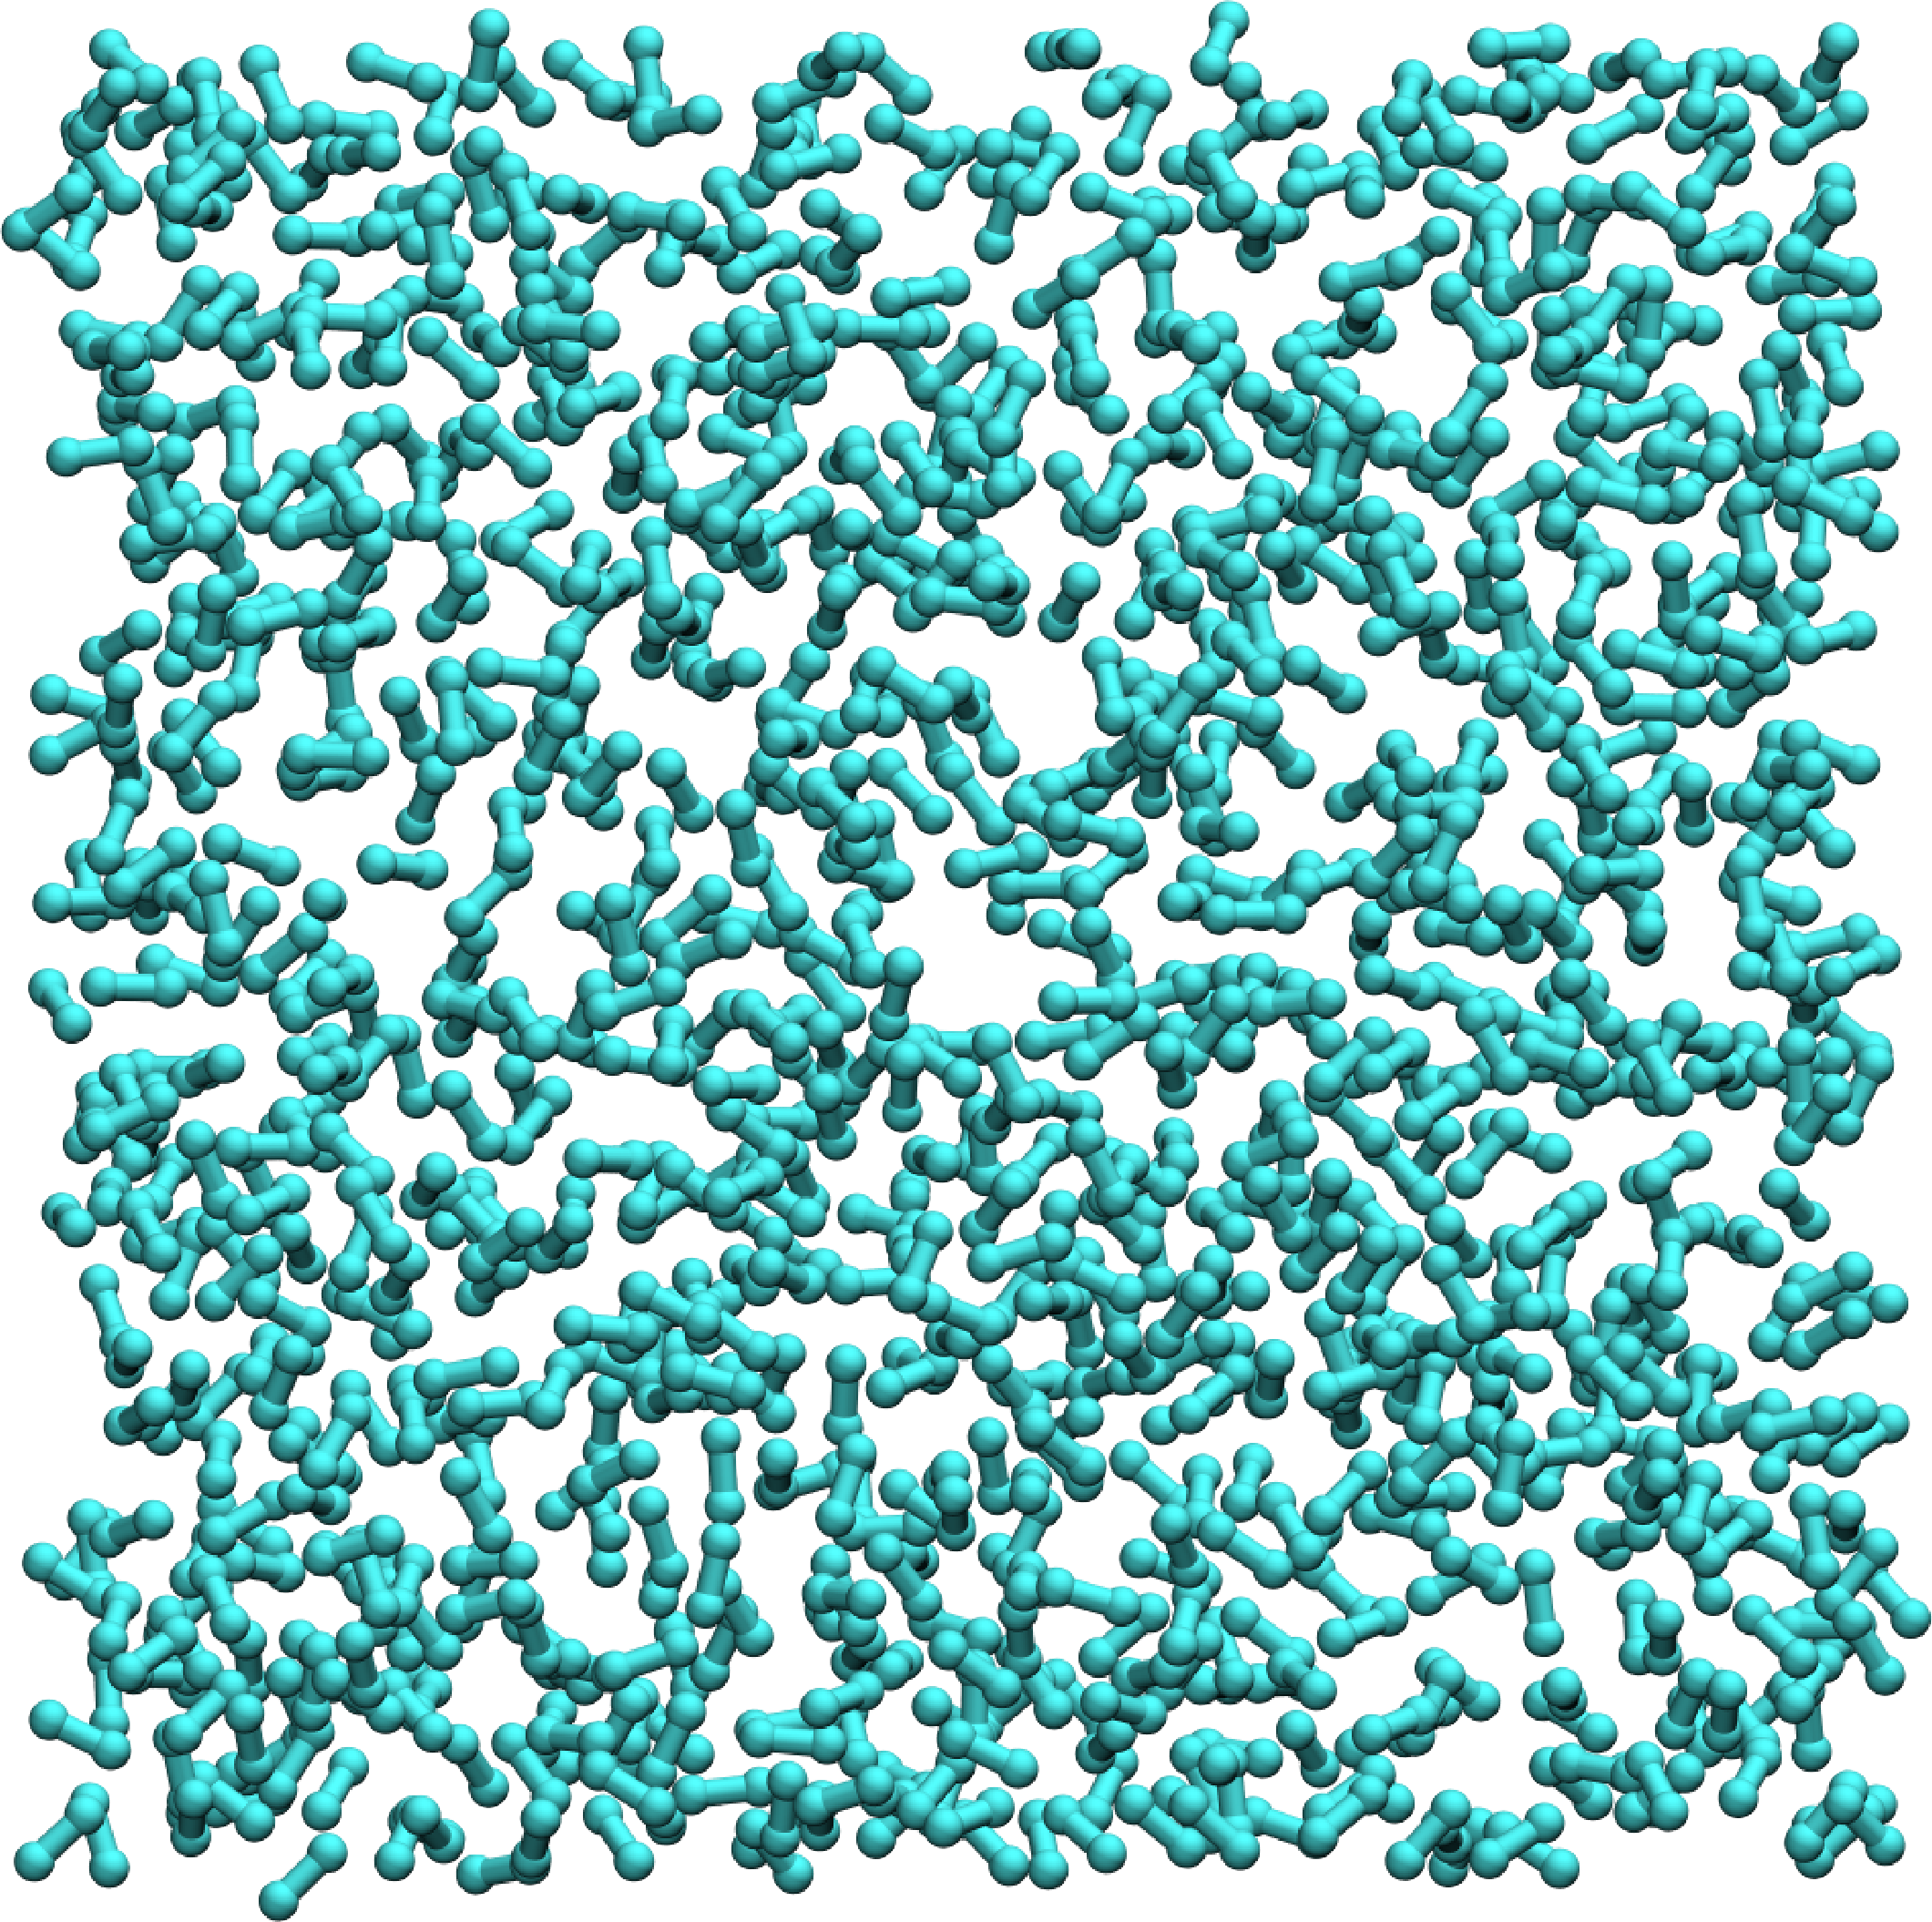
\includegraphics[width=0.48\textwidth]{figures/ArbitraryDiatomixParticlesBox.png}
    \caption{The particles visualised by \code{vmd intro.gro}. With representations set to \textit{dynamic bonds} and \textit{VDW} In the simulation, the bonded atoms are treated as a harmonic oscillator.}
    \label{fig:ArbitraryDiatomixParticlesBox}
\end{figure}
Since the coordinates in \code{intro.gro} are initialized more or less randomly, their positioning might result in overlapping atoms. Thus, starting simulations from such states with very high forces results in unstable MD simulations. Therefore, an initial potential energy minimization using \texttt{em.mdp} removes sterical overlaps to converge to an energetically favorable regime. The downloadable \code{em.mdp} file must thus be used before applying the \code{intro.mdp} file in the following simulation. Commands that conduct the energy minimization and the MD simulation can look like the following lines of code. Their flags and options are detailed in \fref{tab:flagsoptions}.
\begin{lstlisting}[language=bash]
gmx grompp -f em.mdp -p topol_2.top -c intro.gro -o em_2.tpr
gmx mdrun -v -deffnm em_2
gmx grompp -f intro_0.001.mdp -p topol_2.top -c em_2.gro -o intro_0.001_2.tpr -maxwarn 3
gmx mdrun -v -deffnm intro_0.001_2
gmx energy -f intro_0.001_2.edr -o intro_0.001_2.xvg
\end{lstlisting}
\begin{table}[H]
    \centering
    \caption{Each flag given in the code above is explained in detail in this table using one example.}
    \label{tab:flagsoptions}
    \footnotesize
    \begin{tabular}{l p{5cm}}
        \toprule
        Flag (+ Option) & Meaning \\
        \midrule
        \code{-f em.mdp}        & Use the energy minimisation parameter file as \code{grompp} input.\\ \midrule
        \code{-p topol\_2.top}  & In this example, use the system topology with an atomic weight of 2 Dalton.\\ \midrule
        \code{-c intro.gro}     & Use the initial coordinates from the online repository for the energy minimization.\\ \midrule
        \code{-o em\_2.tpr}     & Output the file \code{em\_2.tpr} for usage in the \code{gmx mdrun} command. The name contains the parameter setup (em) and topology info (2). \\ \midrule
        \code{-maxwarn 3}       & Choosing unreasonable options is registered and halted by \texttt{GROMACS}. This safety measure is based on warnings and can be circumvented for didactic purposes via this flag.\\ \midrule
        \code{-v}               & Gives information about the time step and remaining simulation time if the simulation works. If the simulation does not work, there is no timing information.\\ \midrule
        \code{-deffnm em\_2}            & all input and output names of the corresponding \code{gmx mdrun} should have the prefix \code{em\_2} which must match the \code{-o} option of \code{gmx grompp}.\\ \midrule
        \code{-f intro\_0.001\_2.edr}   & Instead of an \texttt{MDP} file for \code{gmx grompp}, \code{gmx energy} needs an \texttt{EDR} file for the \code{-f} flag. The prefix is the same as specified in the \code{-deffnm} option of \code{gmx mdrun}.\\
        \bottomrule
    \end{tabular}
\end{table}
Finally, the task is to choose three different time steps and compare the different outcomes. Firstly, a small time step should be selected so that the system propagates numerically stable. The second case represents a simulation where the energy conservation is violated, but the simulation still finishes. In the last case, the large time step causes the simulation to crash due to numerical instability. In this case, \code{gmx mdrun} will halt, and you have to abort the program with \keystroke{Ctrl}+\keystroke{C}. Eventually, 12 plots will be featured in the report. Three different time steps for each of the four particle masses (e.g. \fref{fig:threets}). 
\begin{figure}
    \centering
    
\includegraphics[width=0.48\textwidth]{figures/threets.png}
    \caption{Example plots for one system. (left panel) total energy vs simulation time for the stable time step, (middle panel) example result for an unstable simulation, where the total energy increases over time, and lastly, a simulation that crashes after \SI{0.06}{\pico\second} due to extremely high forces (\textit{exploding}).}
    \label{fig:threets}
\end{figure}\noindent
It is easy to generate the two extremes, however, an intermediate time step that violates energy conservation but does not crash is challenging to select. Typically, a time step of around \SI{0.001}{\pico\second} is used for classical atomistic MD simulations.\cite{Kim_2014} Start with this time step and the lightest system. Then, increase the time step in steps of \SI{0.001}{\pico\second} until the system crashes or violates energy conservation. If the system crashes, a time step in between the current and the former needs to be tried (e.g., \SI{0.0035}{\pico\second}). Otherwise, if the intermediate case is achieved, the results can be saved, and the next increment can be tried to cause a crash. In order to check the energies, \texttt{xmgrace} or any other plotting utility can be used. Python, via Jupyter Notebook, is also recommended, especially for figures to be featured in the reports. However, for having a quick look at the graphs, \texttt{xmgrace} suffices.
\begin{lstlisting}[language=bash]
xmgrace -nxy output.xvg
\end{lstlisting}
Once all three graphs are ready for the lightest system, the second-lightest system may be tried with the intermediate time step found for the lightest system. As before, the time step has to be incremented or decremented until all three cases are achieved. The same procedure applies to the remaining systems. The graphs and a discussion of the results and apparent trends should be included in the report. Additionally, state what time step you would choose for the respective system.
\newpage

    
\section{Exercise 2: Forcefield Terms and Polymer Statistics}\label{sec:ForceField}
\begin{Checklists}
    \begin{checklist}{Tasks for the Second Exercise}
    \textbf{Finish these tasks and write a short report about your findings.}
    \begin{itemize}
    	\item Compare your analytical solutions for $R_\text{e}$ to the numerical ones.
		
		\item Plot all $R_\text{e}$ and $R_\text{gyr}$ vs. the simulation time.
		
		\item Include histograms of the $\theta$ and $\phi$ and plot the chain averages vs. simulation time.
		
		\item Summarize all averages for $\theta$, $\phi$, $R_\text{gyr}$ and $R_\text{e}$ in \textit{one} table.
		
		\item Describe and interpret your results. Include representative snapshots generated by \texttt{VMD} to support your conclusions.
    \end{itemize}
    \end{checklist}
\end{Checklists}

\begin{figure}[H]
    \centering
    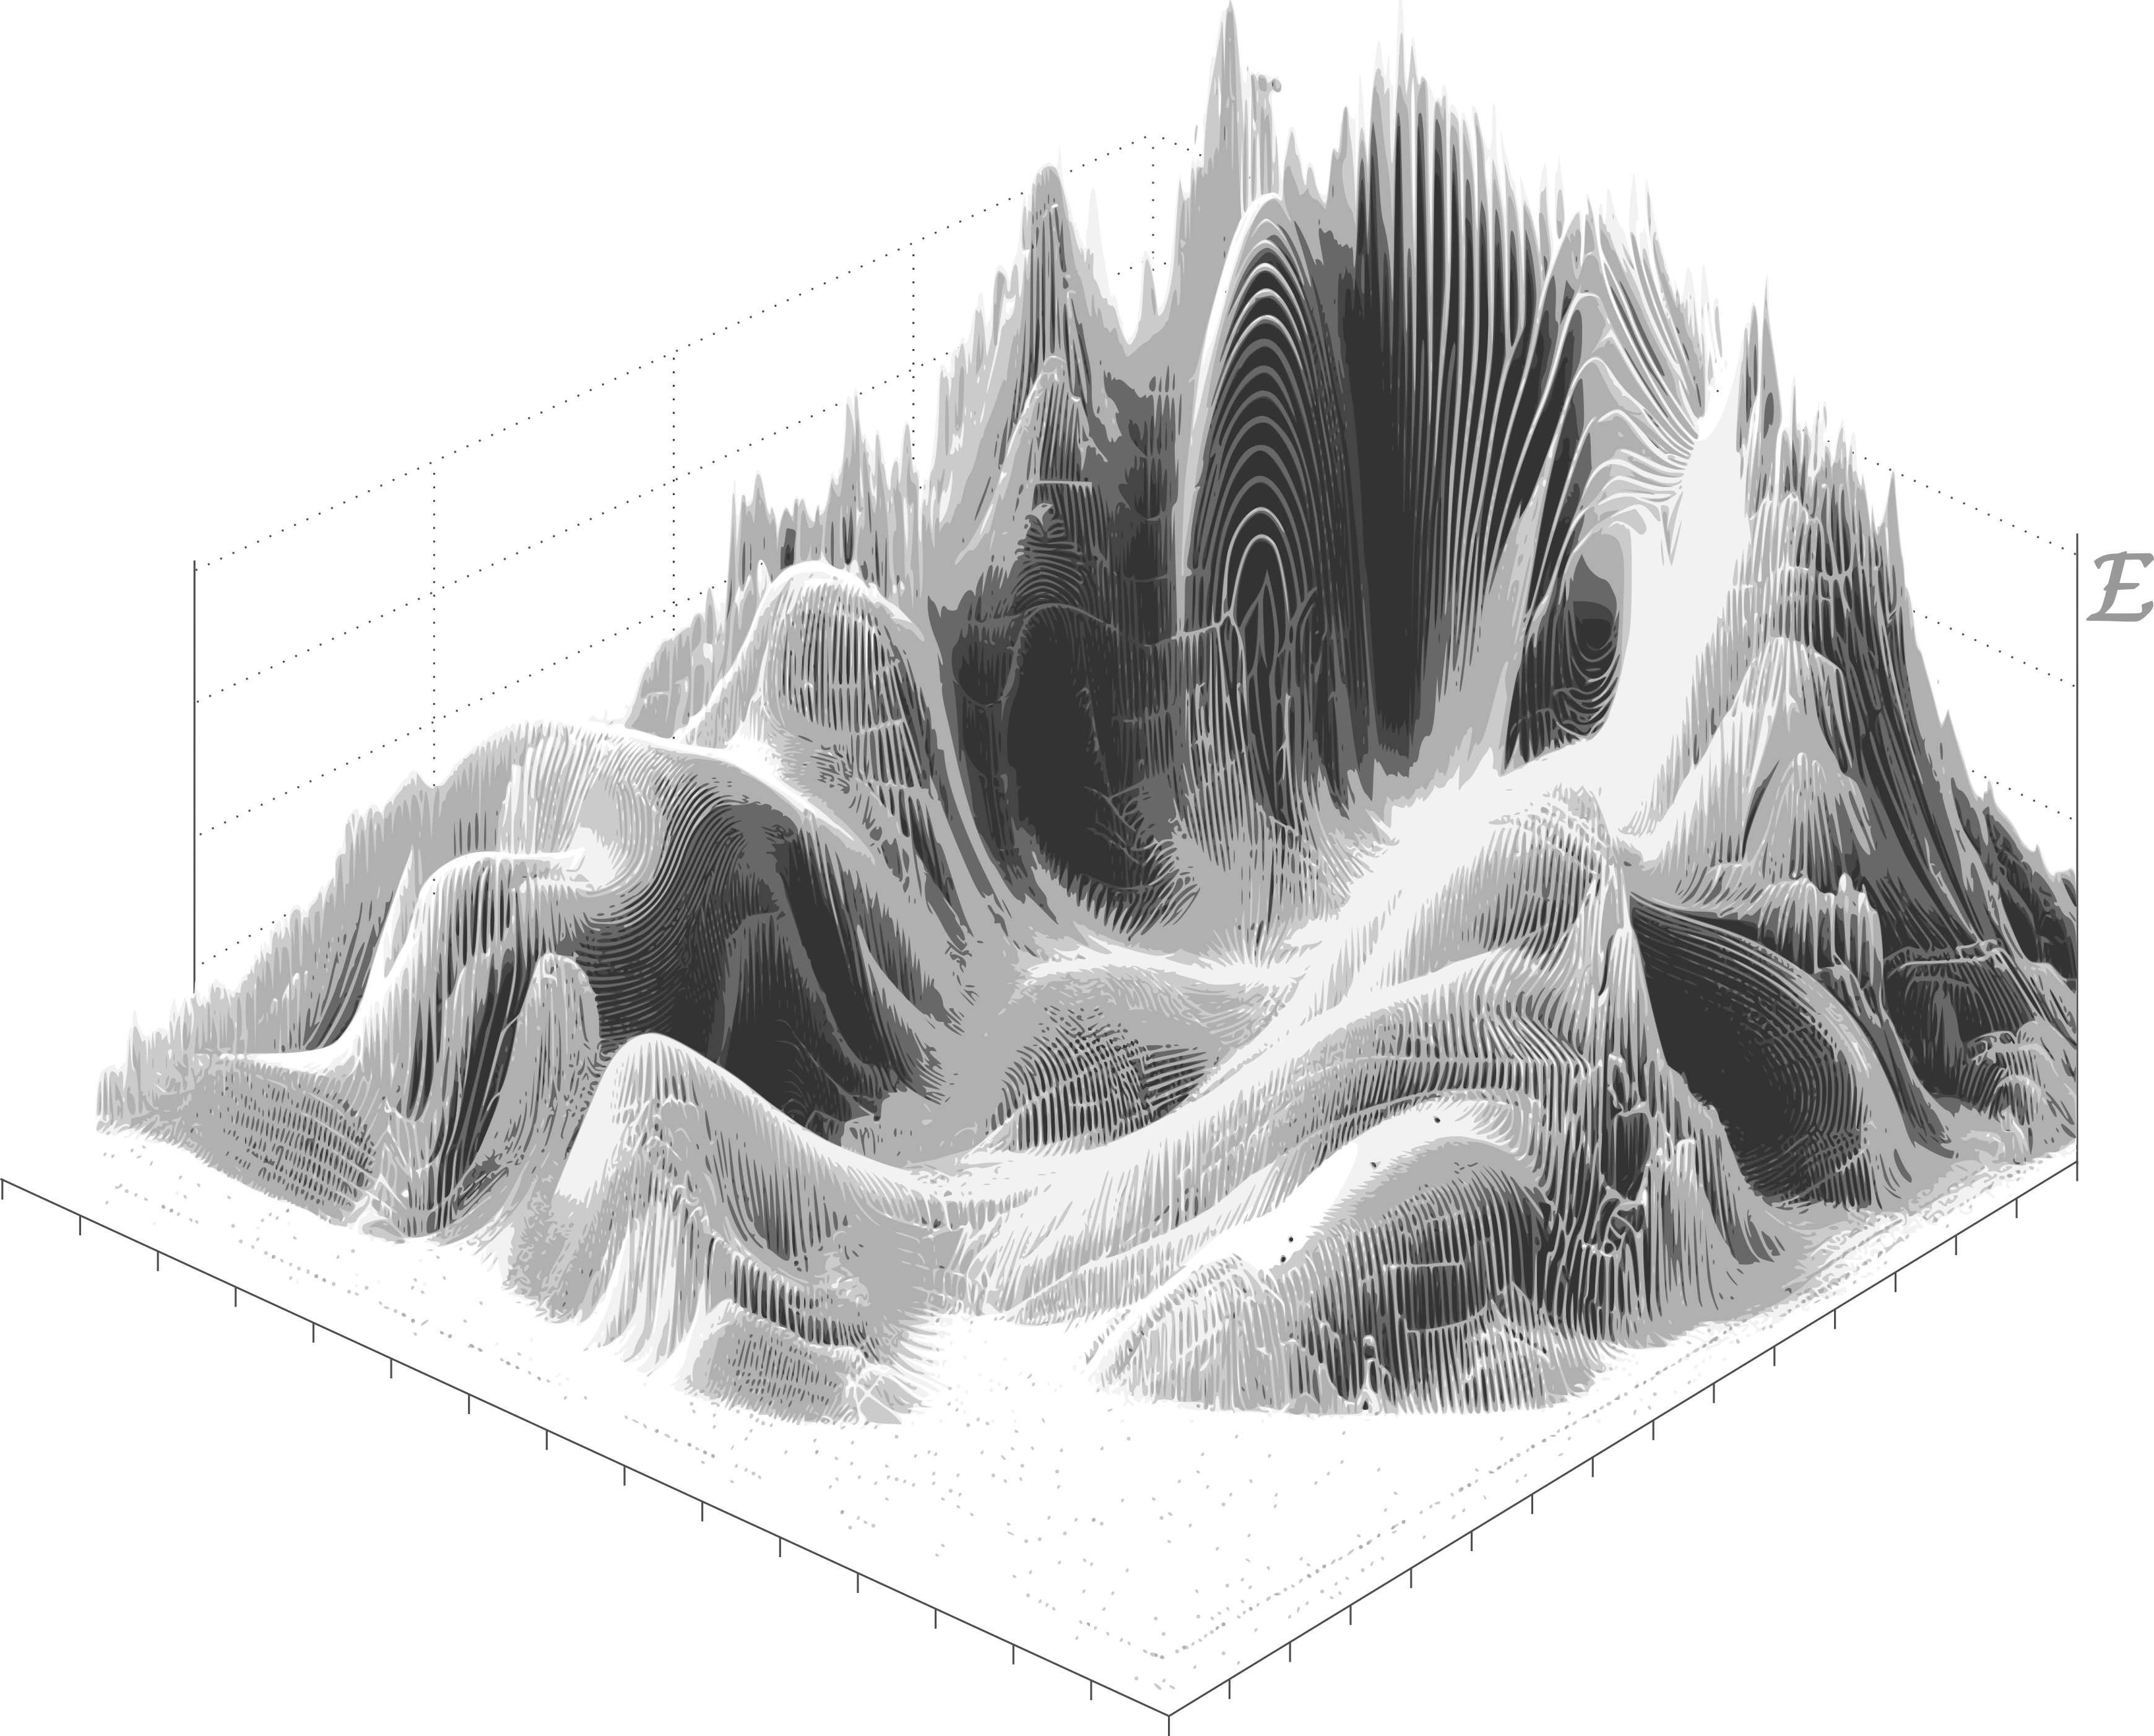
\includegraphics[width=0.48\textwidth]{figures/PES_concept.png}
    \caption{Conceptual depiction of the potential energy surface. The real potential energy surface is (3N-6)-dimensional and cannot be illustrated in 2D.}
    \label{fig:PES_concept}
\end{figure}
Molecular dynamics (MD) simulations are a unique method that enables the user to visualize time-resolved processes in atomic detail. However, the method only approximates reality by parametrizing molecular properties, e.g., charges and bond lengths. The complete set of these parameters and their respective formulas is called \textit{forcefield}, synonymous with the system's potential energy. The quality of the forcefield, as well as its completeness, determines the quality of an MD simulation's predictions. In this exercise, a simple polymer consisting of carbon atoms is simulated with different levels of forcefield completeness. The goal is to better understand the forcefield terms and their implementation in \texttt{GROMACS}. Additionally, a comparison with analytical polymer models will be conducted. 


\subsection*{Theoretical Considerations}
The complete (polymer) forcefield $U_\text{\tiny tot}$ can be split into an intramolecular term $U_\text{intra}$ and an intermolecular term $U_\text{inter}$. 
\begin{align}
U_\text{\tiny tot} & =  U_\text{\tiny inter} + U_\text{\tiny intra}
\end{align}
On the one hand, $U_\text{\tiny intra}$ consists of bond, angular and dihedral contributions. The bonded potential $U_\text{b}$ and the angular potential $U_\theta$ are harmonic potentials and therefore defined by an equilibrium distance $b_0$ and angle $\theta_0$ as well as a force constant $k_\text{b}$ and $k_\theta$. Usually, the dihedral term is a cosine potential defined by the force constant $k_\phi$, phase $\phi_0$ and periodicity $n_\phi$.
\begin{align}
U_\text{\tiny intra} & = \sum_{i}^{\text{\tiny bonds}} U_\text{b}(b_i) + \sum_{j}^{\text{\tiny angles}} U_\theta (\theta_j) + \sum_{k}^{\text{\tiny dihedrals}} U_\phi (\phi_k)\\
U_\text{b}(b_i) & = k_\text{b} \left(b_i -b_0\right)^2\\
U_\theta(\theta_j) & = k_\theta \left(\theta_j -\theta_0\right)^2\\
U_\phi(\phi_k) & = k_\phi \left(1 + \cos\left(n_\phi\phi_k - \phi_0\right)\right)
\end{align}
On the other hand, $U_\text{inter}$ only consists of the Lennard-Jones potential $U_{\varepsilon,\sigma}$, depending on the parameters $\varepsilon$ and $\sigma$ and the interatomic distance $r_{mn}$.
\begin{align}
	U_\text{\tiny inter} & = \sum_{m}^{\text{\tiny Atoms}} \sum_{n\neq m}^{\text{\tiny Atoms}} U_{\varepsilon,\sigma}(r_{mn})
\end{align}
The Lennard-Jones potential is one of many standard potentials implemented in \texttt{GROMACS}, and the interpretation of its parameters is quite intuitive. $\varepsilon$ corresponds to the potential well depth, and $\sigma$ indicates the particle radius, which could be shown from its mathematical expression.\cite{LennardJones1924}
\begin{align}\label{eq:lennardJones}
	U_{\varepsilon,\sigma}(r_{mn})= 4 \varepsilon \left [ {\left (\dfrac{\sigma}{r_{mn}} \right )}^{12}-{\left (\dfrac{\sigma}{r_{mn}} \right )}^{6} \right]
\end{align}
An important potential herein omitted is the Coulomb potential, which describes charge-charge interactions. The potential energy function $U_\text{\tiny tot}$ has already been introduced in the calculation of forces in \fref{eq:NewtonsEqOfMotion} in the previous exercise. That means for each numerical integration time step the forcefield must be used to calculate all forces acting on each particle. The intramolecular part is computationally less expensive than the intermolecular forcefield, due to the double sum over all Lennard-Jones interactions. The herein omitted electrostatic interactions feature a double sum as well.\\
For a polymer consisting of $N$ beads at positions $\vec{b}_{1}$ to $\vec{b}_N$ the mean squared end-to-end distance of the polymer chain $\langle R^2 \rangle$ can be calculated using the formula below.
\begin{align}\label{eq:Re2e}
	\langle R_\text{ee}^2 \rangle &= \langle R_\text{ee} \cdot R_\text{ee} \rangle = \langle \sum_i r_i \sum_j r_j \rangle = \sum_i \sum_j \langle  r_i \cdot r_j \rangle 
\end{align}
Analytical formulas $\langle R_\text{ee}^2 \rangle$ can be derived for the freely jointed and freely rotating polymer models. The former is defined only by a fixed bond length $L$, while the latter also features a fixed angle $\theta$ between adjacent beads. Calculating the analytical solutions for both polymer models, followed by comparison to MD simulations, is an adequate way to assess the validity of the simulations.


\subsection*{Setup and Simulations}
In this exercise, a polymer consisting of 20 atoms should be simulated in the NVT ensemble for the following cases:
\begin{enumerate}
	\item freely jointed chain; only $U_\text{b}$ is active.
	\item freely rotating chain; $U_\text{b}$ and $U_\theta$ are active.
	\item complete intramolecular forcefield; $U_\text{\tiny intra}$ is active.
	\item complete forcefield; $U_\text{\tiny tot}$ is active with $\varepsilon=\SI{0.9786}{\kilo\joule\per\mole}$ and $\sigma=\SI{0.3401}{\nano\meter}$.
\end{enumerate} 
The individual contributions to the forcefield are specified in the topology file, herein called \code{polymer.top}. It can be downloaded from the online repository and should be briefly inspected. Activating the demanded forcefield terms requires deleting the \code{;} in the \texttt{TOP} file in front of the respective lines. The \code{;} precedes comments that are not interpreted by \texttt{GROMACS}. The parameters for $U_\text{\tiny inter}$ can be set in the \code{[ atomtypes ]} section.\\
% Simulation process
As a reminder, \texttt{GROMACS} requires you to execute \code{gmx grompp} and \code{gmx mdrun} to perform a simulation. Furthermore, consistent names should be chosen for simulation files to keep directories neat. A command prompt for the freely jointed simulation could look like this:
\begin{lstlisting}[language=bash]
gmx grompp -f polymer.mdp -c polymer.gro -p polymer_fj.top -o polymer_fj.tpr
gmx mdrun -deffnm polymer_fj -v
\end{lstlisting}
\begin{figure}
    \centering
    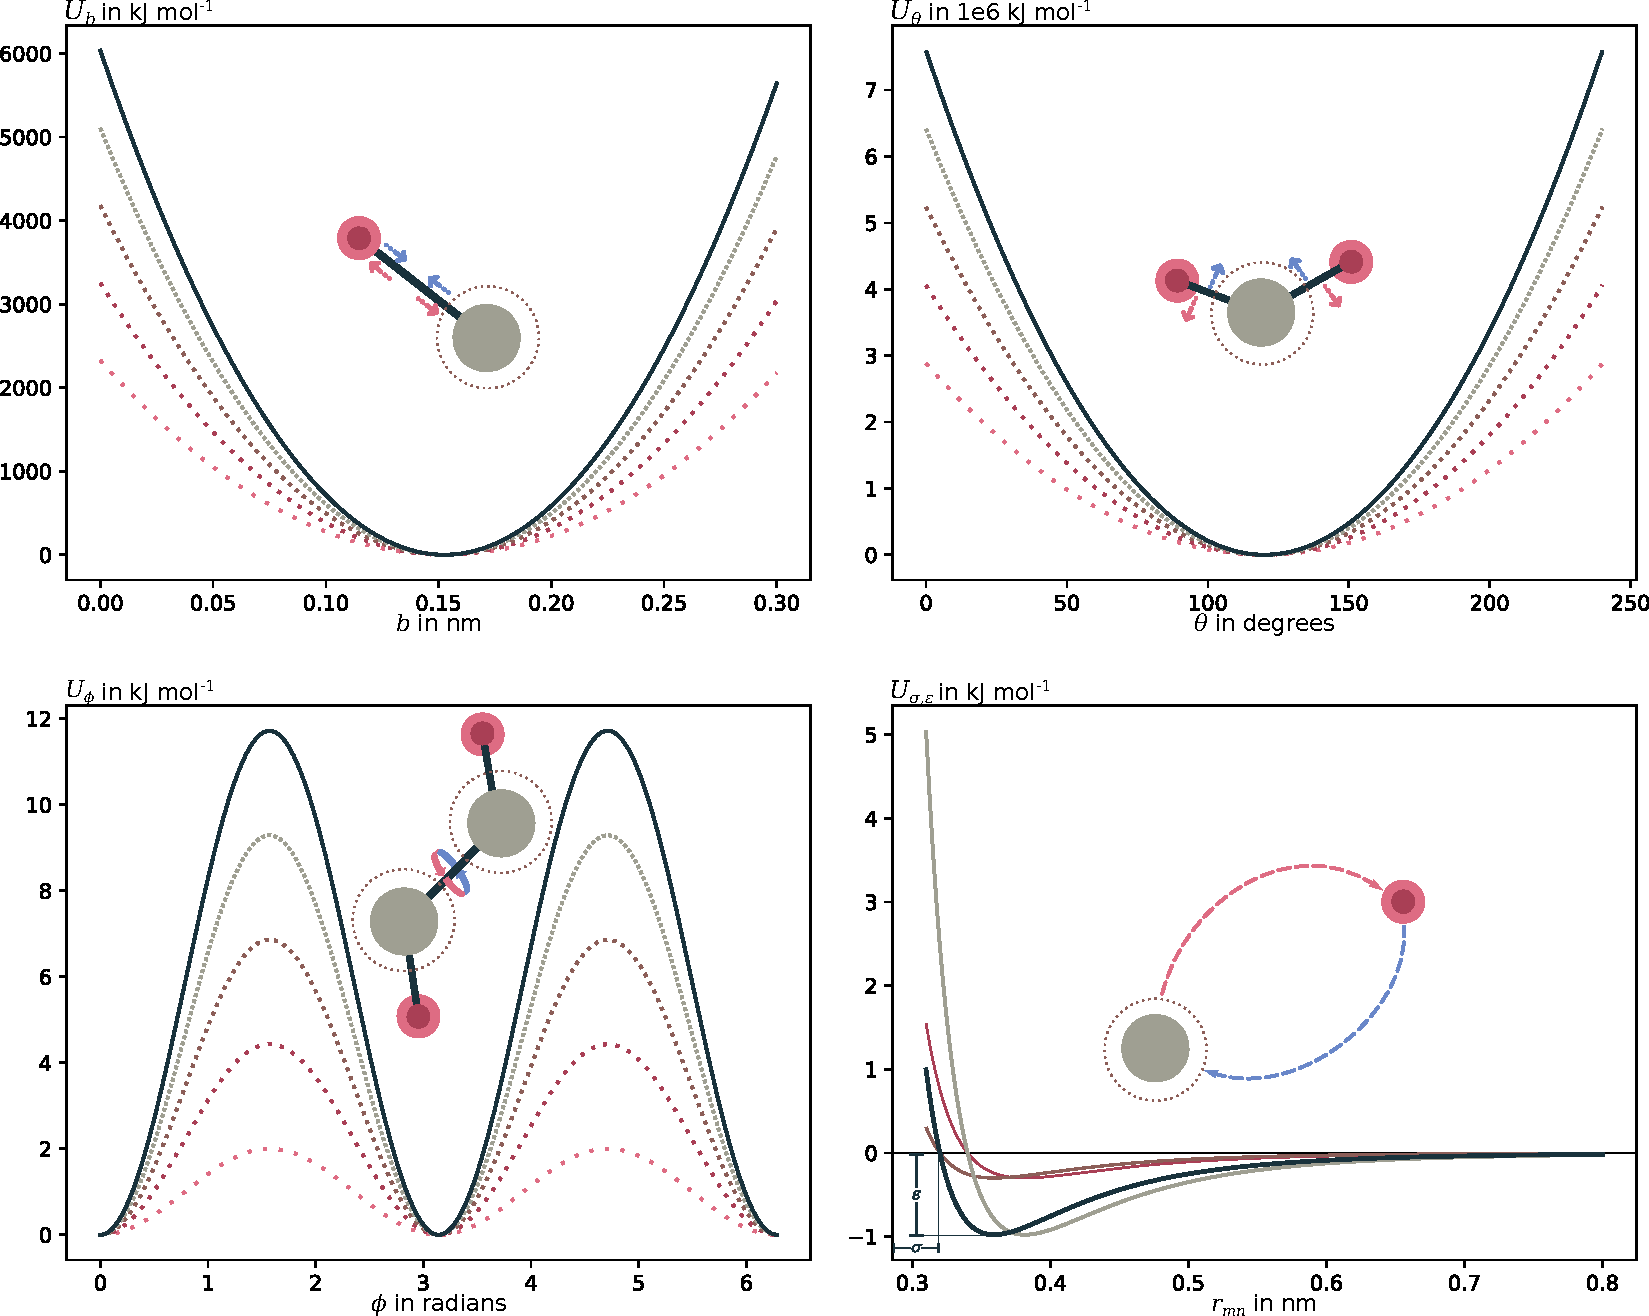
\includegraphics[width=0.48\textwidth]{figures/forcefieldterms.pdf}
    \caption{Exemplary plots of each forcefield term. The bonded potential is plotted on the upper left, followed by angular, torsional, and non-bonded potential. The colored, dotted lines in each panel depict the same forcefield term of decreasing strength (force constant). In the case of the non-bonded potential, this trend is visualized via the line width for aesthetic reasons. Furthermore, the epsilon and sigma values of the strongest potential are annotated close to the origin. Notice the differences in the energy scale of each contribution.}
    \label{fig:ffterms}
\end{figure}


\subsection*{Analysing the Trajectory}
Once all simulation runs are finished, the trajectories need to be analyzed. Herein, angular properties and statistical polymer properties should be calculated. \texttt{GROMACS} offers the built-in tools \code{gmx polystat} and \code{gmx angle} for this purpose.
% Angular properties
Since the angular potentials $U_\theta$ and $U_\phi$ are not included per default, their impact on the carbon chain should be investigated. Therefore, the average angle should be plotted vs. the simulation time. Additionally, an angle histogram should be generated. Both plots can be done by \texttt{GROMACS} via \code{gmx angle}. However, this command needs information about the triplets involved in one angle provided in a custom \texttt{NDX} file. This file lists the atom numbers making up each angle in the simulation. Therefore, it can be repurposed once it is generated. Luckily, \texttt{GROMACS} has a separate command, \code{gmx mk\_angndx}, that outputs such a file automatically if angular information is present in the input \texttt{TPR} file. For example, for the freely jointed simulation, the necessary plots can be generated using the following commands:
\begin{lstlisting}[language=bash]
gmx mk_angndx -s polymer_full.tpr -n angle.ndx -type angle
gmx angle -f polymer_fj.xtc -n angle.ndx -od fj_angle_hist.xvg -type angle -ov fj_angle.xvg
\end{lstlisting}
The same steps must be taken to plot the dihedrals for the report. Thus, \code{gmx mk\_angndx} must be executed but with the correct \code{-type} option, followed by the command \code{gmx angle}. The procedure is analogous to the one showcased above. Plotting the histograms of the individual forcefield cases into one plot is recommended to clarify differences.\\
% statistic polymer properties
\begin{figure}[H]
    \centering
    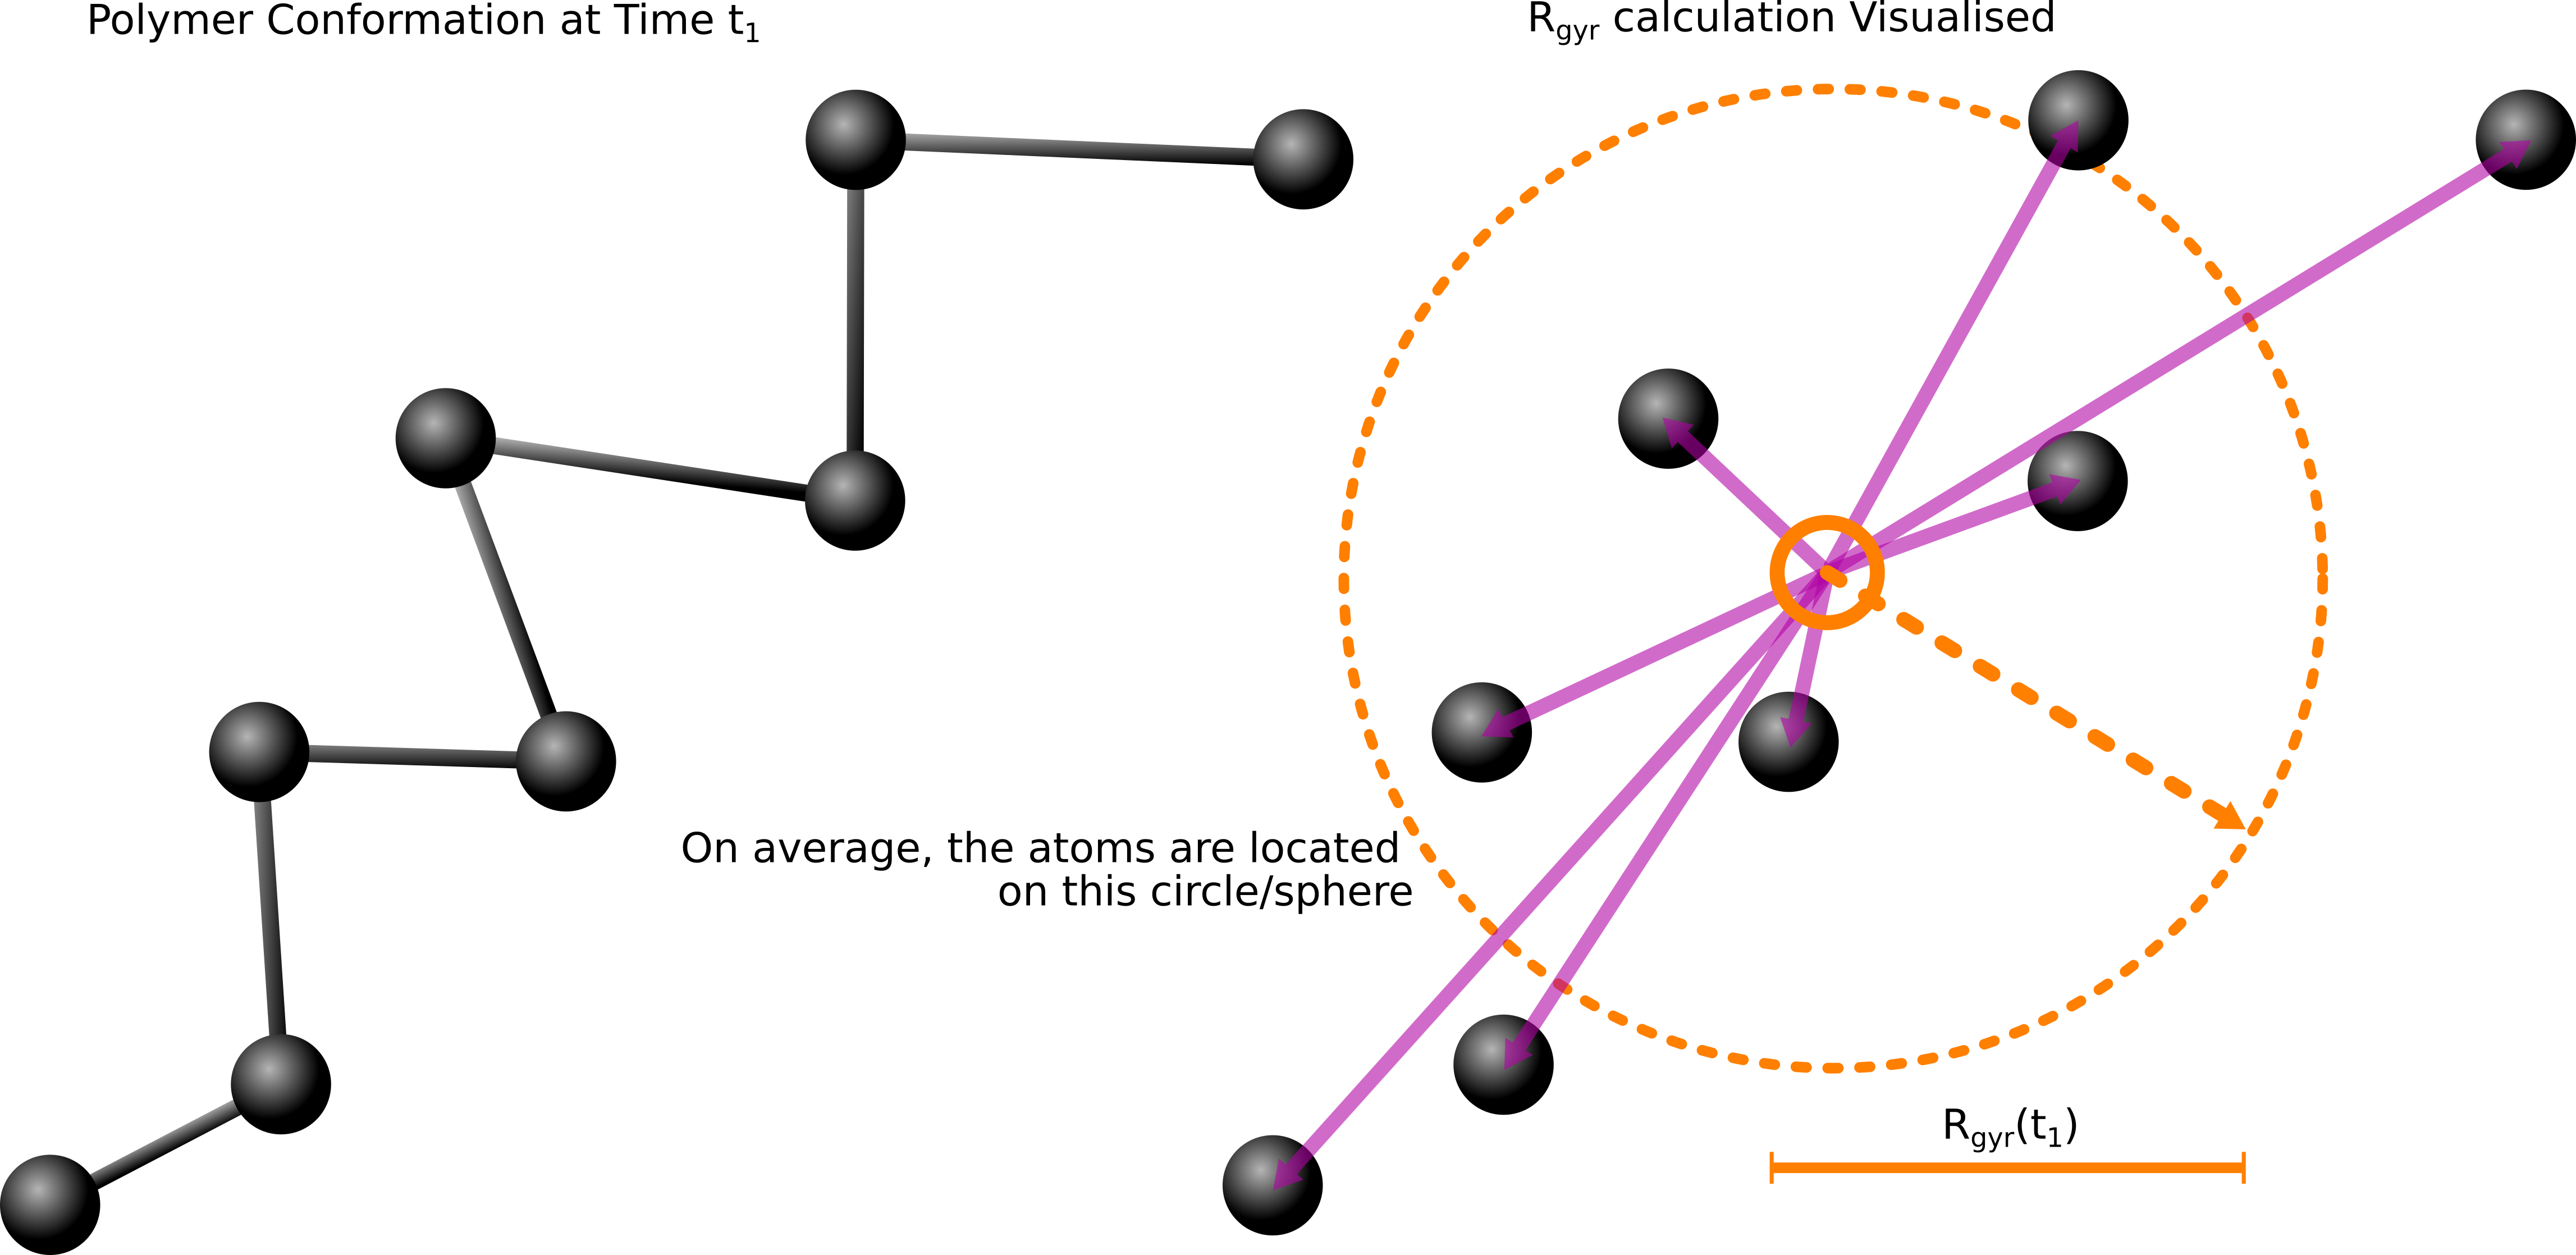
\includegraphics[width=0.48\textwidth]{figures/rgyr.png}
    \caption{Visualisation of the calculation for $R_\text{gyr}$: only the atomic distances to the center of geometry of a given conformation are measured and then averaged. For extended conformations, $R_\text{gyr}$ is larger than for collapsed polymer chains. However, for an equilibrated ensemble, a static ensemble average emerges $\langle R_\text{gyr}\rangle$.}
    \label{fig:rgyr}
\end{figure}
The average end-to-end distance $\overline{R_\text{ee}}$ of the simulations can be validated using analytical results for comparison. From \fref{eq:Re2e} analytical formulas shall be derived to calculate the root mean square end-to-end distance $\sqrt{\langle R_\text{ee}^2 \rangle}$ for the freely jointed and the freely rotating polymer model. These calculations should agree with the numerical results obtained from simulation. As aforementioned, \texttt{GROMACS} has its built-in tool to calculate $\overline{R_\text{ee}}$ and $\overline{R_\text{gyr}}$. Example code is given below.
\begin{lstlisting}[language=bash]
gmx polystat -s polymer_fj.tpr -f polymer_fj.xtc -o fj_polystat.xvg
\end{lstlisting}
For the report, the time averages $\overline{R_\text{ee}}$ and $\overline{R_\text{gyr}}$, plots that feature their time development and the analytical results shall be included. All measurements should be summarised in a table for a better overview of the results. The analytical and numerical results for $R_\text{ee}$ and their agreement should be discussed. Also, similarities and differences between the different simulations should be discussed concerning the underlying forcefield terms. Visual proof drawn from \texttt{VMD} may be incorporated.


\subsection*{Tutorial on Visualising a Trajectory}
A standard visualization program used for molecular dynamics simulation is called \texttt{VMD}. For simulation output generated by \texttt{GROMACS}, you have to input the \texttt{GRO} file and the \texttt{XTC} file to visualize trajectories. The \texttt{GRO} file only specifies the atom configuration, while \texttt{VMD} guesses the bonds. Therefore, matching \code{polymer\_fj.gro} and \code{polymer\_fj.xtc} files may incorrectly depict molecular bonds. Instead \code{polymer.gro} can be used.
\begin{lstlisting}[language=bash]
vmd polymer.gro polymer_fj.xtc
\end{lstlisting}
Since the \texttt{VMD} defaults, when loading a trajectory, can be suboptimal follow the steps below for an improved trajectory appearance. Firstly, the visibility is greatly enhanced by aligning the structure (see \fref{fig:tut1}). Aligning entails centering the structure of each time frame on the reference frame coordinates, followed by rotations that minimize the atomic distances between the two frames. This operation makes the trajectory appear less juddery.\\
\begin{figure}[H]
	\centering
	
\includegraphics[width=0.48\textwidth]{figures/tutorial1.png}
	\caption[aligning the molecule]{\code{Extensions} $\Rightarrow$ \code{Analysis} $\Rightarrow$ \code{RMSD Trajectory Tool} $\Rightarrow$ \texttt{window opens} $\Rightarrow$ \code{Align} $\Rightarrow$ \texttt{close the window}}
	\label{fig:tut1}
\end{figure}
Secondly, the representation of the molecule per default is set to lines, which lacks visibility. Changing this to \texttt{Licorice} and applying Gaussian smoothing to the trajectory enhances the user experience even further (see  \fref{fig:tut2}). 
\begin{figure}[H]
	\centering
	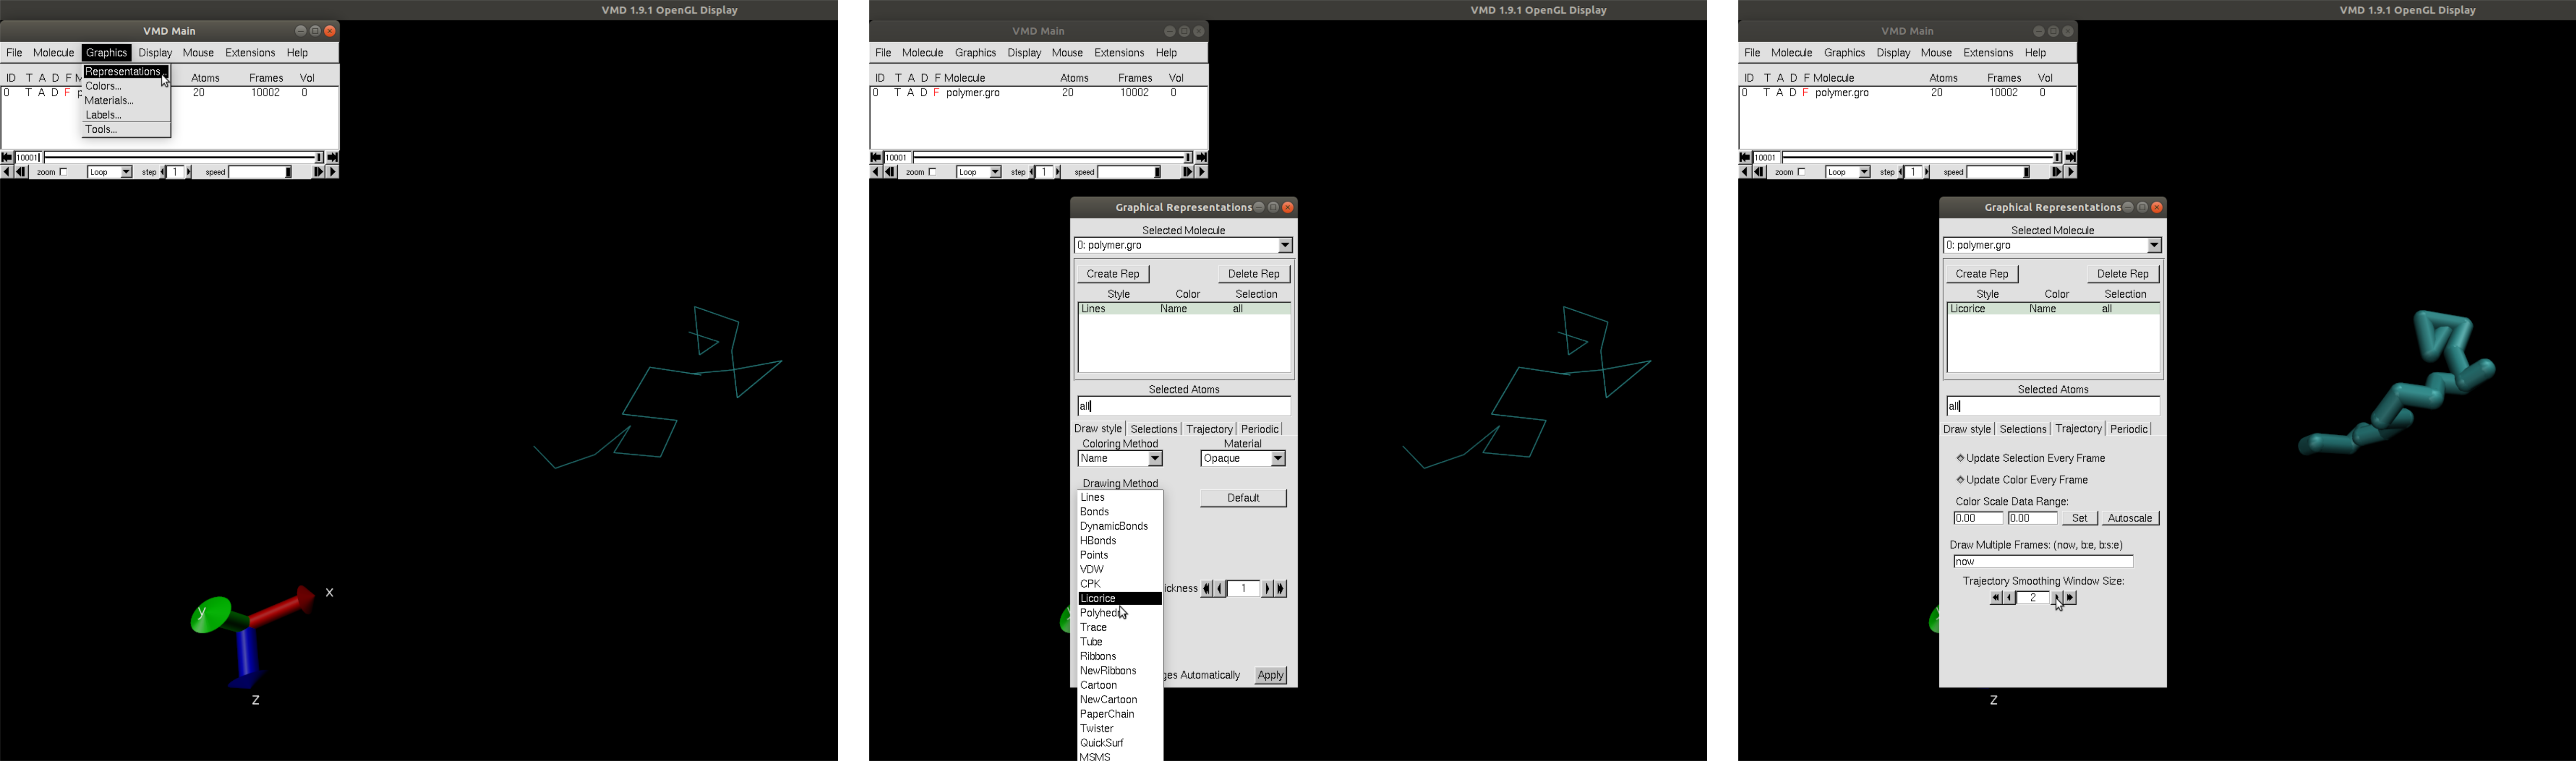
\includegraphics[width=0.48\textwidth]{figures/tutorial2.png}
	\caption[better drawing style]{\code{Graphics} $\Rightarrow$ \code{Representations} $\Rightarrow$ \texttt{window  opens on Tab} \code{Draw Style} \\$\Rightarrow$ \code{Drawing Method} $\Rightarrow$ \code{Licorice}  ($\Rightarrow$ \texttt{optional: adjust Bond Radius}) $\Rightarrow$ \texttt{switch Tab to} \code{Trajectory} $\Rightarrow$ \texttt{set} \code{Trajectory Smoothing Window Size} \texttt{to 3} $\Rightarrow$ \texttt{Close the Window}}
	\label{fig:tut2}
\end{figure}
For including snapshots in the report, the \code{Trajectory} \code{Smoothing} \code{Window} \code{Size} must be reverted to zero since this setting manipulates the atom positions. The easiest and quickest way to generate images from \texttt{VMD} is to take screenshots.

\newpage

\section{Exercise 3: Temperature Coupling and Heat Capacity}\label{sec:tcoupling}
\begin{Checklists}
    \begin{checklist}{Tasks for the Third Exercise}
    \textbf{Finish these tasks and write a short report about your findings.}
    \begin{itemize}
		\item Include a commented thermostat-\texttt{MDP} file of your choice.
		\item For all six production runs, plot $T$, $E_\text{kin}$, $E_\text{tot}$ and $E_\text{pot}$ vs simulation time and describe them. Particularly, find differences and similarities between the thermostats.
		\item Calculate and compare the $C_\text{v}$ of each production run with the literature value and interpret the results.
		\item Visualize the polymer trajectory with \texttt{vmd} and describe any unusual behavior. You may include screenshots of representative conformations. 
		\item Compare the \texttt{MDP} file from the current simulation with the previous exercise's \texttt{MDP} file and speculate which alterations might have caused the behavior at hand.
	\end{itemize} 
\end{checklist}
\end{Checklists}
\begin{figure}[H]
    \centering
    
\includegraphics[width=0.48\textwidth]{figures/Flying-Ice-Cube.png}
    \caption{Cartoon Depiction of the Flying-Ice-Cube effect. Adapted from DALL-E.}
    \label{fig:Flying-Ice-Cube}
\end{figure}


\subsection*{Introduction}
Up to this exercise, the simulations have been conducted without emphasizing the system temperature. Most of the simulations were conducted in the microcanonical ensemble with a constant number of particles (N), constant volume (V), and constant total energy (E), also called the NVE ensemble. Implementing temperature control includes coupling the molecular system to a virtual heat bath, allowing energy exchange. Therefore, the canonical ensemble features a constant number of particles, volume, and temperature. It is also called the NVT ensemble.\cite{Hnenberger2005} Adding a level of temperature control to Newton's second law, thus switching to the canonical ensemble, might be desirable for various reasons. Some include matching an experimental setup, studying thermosensitive processes, and exploring the sampling space more time-efficiently with advanced methods (e.g., temperature replica exchange molecular dynamics simulations\cite{Swendsen1986,Sugita1999}).\\
This exercise is structured in two parts. In the first part, simulations shall be setup to compare different thermostatting algorithms and their effect on different water forcefields. The second part only consists of a visual analysis of a trajectory featuring the flying-icecube-effect. This exercise aims to become familiar with different water models, visualize MD trajectories, and independently assess the drawbacks and benefits of popular thermostats by calculating the isochoric heat capacity and comparing it to its experimental values. This way, the accuracy of the thermostats and the water models can be analyzed. 


\subsection*{Theoretical Considerations}
Within MD simulations, different temperature concepts are distinguished via nomenclature. Firstly, the instantaneous temperature $T$ is obtained from the atomic velocities of each simulation time step.
\begin{align}
    T(t) = \frac{1}{3Nk_\text{B}} \sum_i^N m_i v_i(t)^2
\end{align}
Secondly, the ensemble average of the temperature $\langle T \rangle_\text{NVT}$ is a thermodynamic constant approximated by the system's time average, assuming thermodynamic equilibrium and sufficient sampling time.\cite{Coudene2016}
\begin{align}
    \langle T\rangle_\text{\tiny NVT}  \approx \frac{1}{t_1 - t_0} \int_{t_0}^{t_1} \frac{1}{3Nk_\text{B}} \sum_i^N m_i v_i(t)^2 dt
\end{align}
Finally, the reference temperature, $T_0$, is the heat bath temperature imposed on the MD system and is a user-specified parameter. Algorithmically, the heat bath's implementation is called a thermostat, a variety of which have emerged over the past decades. To showcase their function, the mathematical framework of the Berendsen thermostat\cite{Berendsen1984} shall be laid out. It is also denoted as \textit{weak coupling} thermostat.\\
The Berendsen thermostat is a widely used, relatively simple thermostat that employs a first-order relaxation equation. This thermostat induces a temperature change that scales proportionally with the difference between reference and instantaneous temperatures and with the coupling parameter $\tau_\text{\tiny T}$.
\begin{align}
    \frac{dT}{dt} & = \frac{1}{\tau_\text{\tiny T}}\left(T_0 - T \right) \\
   \text{ or } \Delta T & = \frac{\Delta t}{\tau_\text{\tiny T}}\left(T_0 - T \right) 
\end{align}
In the context of the numerical integration of Newton's second law, a thermostat is usually implemented by rescaling the atomic velocities since the instantaneous temperature depends on them. It can be shown that the above equations yield the following scaling law for the Berendsen thermostat.\cite{Hnenberger2005}
\begin{align}
    v_i(t) & = v_i^\prime (t) \cdot \sqrt{1 + \frac{\Delta t}{\tau_\text{\tiny T}}\left( \frac{T_0}{T(t)} - 1\right)}
\end{align}
By rescaling the atomic velocities $v_i^\prime (t)$, the Berendsen thermostat ensures that the temperature approaches $T_0$ following an exponential decay. Each thermostat offers certain benefits and drawbacks. A benefit of the Berendsen thermostat is its computational efficiency. Although a thermostat's quality may also be assessed with respect to time-reversibility or consistency with experimental results.\cite{Hnenberger2005,Braun_2019}\\
The isochoric heat capacity $C_\text{v}$ is a material property that relates the amount of applied energy to the increase of temperature. Herein, $C_\text{v}$ is used to measure the quality of the canonical ensemble generated by the temperature coupling algorithm. \texttt{GROMACS} calculates $C_\text{v}$ from the total energy fluctuations $\text{RMSD}(E_\text{tot})$ the specified molecule number $N_\text{mol}$, the ideal gas constant $R$ and the temperature $T$.\cite{Allen1990}
\begin{align}
	C_\text{v} & = \frac{\left(\text{RMSD}(E_\text{tot}) \cdot 1000 \right)^2 \cdot N_\text{mol}}{RT^2}
\end{align}

\subsection*{Setup and Simulations}
\subsubsection*{Comparing different Temperature Coupling Algorithms}
The assessment of two very common thermostats is the subject of this exercise. Herein, the Berendsen and the Nose-Hoover thermostat\cite{Nos1983,Nos1984,Hoover1985} shall be investigated. In the online repository, all necessary input files can be found. These files comprise two different water models and three different temperature coupling algorithms, and they can thus be used to perform six different simulation sequences. In the context of an MD simulation, the water model means the collection of forcefield terms describing a its intramolecular and intermolecular interactions. Similar to the polymer model in the last exercise the simulation sequence consists of an energy minimization, an equilibration, and a production run.\cite{Braun_2019}\\
% MDP Files
This exercise task features six different \texttt{MDP} files: \code{eq\_nve.mdp}, \code{prod\_nve.mdp}, \code{eq\_berendsen.mdp}, \code{prod\_berendsen.mdp}, \code{eq\_nhc.mdp} and \code{prod\_nhc.mdp}. They can be categorized into equilibration \texttt{MDP} files and production \texttt{MDP} files. The simulations utilizing the equilibration \texttt{MDP} files feature fewer timesteps than the production. The purpose is to heat up the system and let it settle into its thermodynamic equilibrium such that the production run starts from an equilibrated system. Eventually, the production \texttt{MDP} files and their respective simulations serve the purpose of data collection. The data of interest are equilibrium properties, and their accuracy typically increases with the simulation length. Therefore, each production simulation takes quite some time to finish, and only the production output files will be used for calculating $C_\text{v}$ and other properties. \\ \\
% Thermostat 
Additionally, the six \texttt{MDP} files can be categorized by the thermostat used during the simulations. The three temperature-coupling algorithms used here are: \texttt{None} (NVE-Ensemble), \texttt{Berendsen}, and \texttt{Nose-Hoover-Chain}. They all perform very differently in generating the correct canonical ensemble, which is connected to the heat capacity. The NVE simulation is supposed to perform worst since it resembles the wrong ensemble all together.\\
Comparing the \texttt{MDP} files via \code{vimdiff <file1> <file2>} should indicate how \texttt{GROMACS} implements the different thermostats and, therefore, the different ensembles. Furthermore, for an advanced understanding of the \texttt{MDP} files, go through each line and explain its meaning via a comment. Consultation of the \texttt{GROMACS} MDP options documentations is recommended (see \url{manual.gromacs.org/documentation/2018/user-guide/mdp-options.html}). Comments can be inserted into an \texttt{MDP} file with \code{; <Comment>}. After commenting, a line could look like the following:
\begin{lstlisting}[language=bash]
intergrator = md ; Leap-Frog algorithm for time integration
\end{lstlisting}
\texttt{GROMACS} will ignore everything behind the semi-colon. Include one completely commented \texttt{MDP} file in your report.\\ \\
\begin{figure}[H]
    \centering
    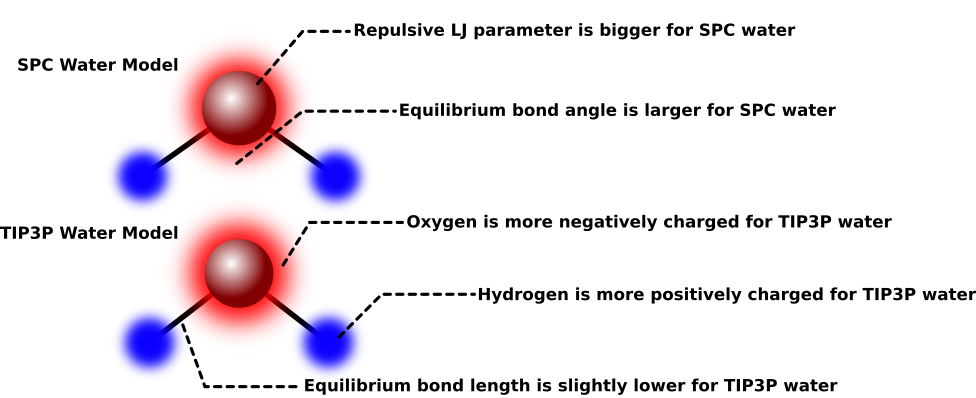
\includegraphics[width=0.48\textwidth]{figures/watermodels.png}
    \caption{TIP3P and SPC water in comparison. The bond lengths, angles, charges, and Lennard-Jones parameters are true to scale and depicted by the different features of each molecule. The blue and red blurs depict the charge, and the red bubble depicts the repulsive Lennard-Jones parameter. Even though the differences are hardly visible, the impact on the accuracy is immense and highlights the importance of precise parameterization in MD. The exact parameters are listed elsewhere (see below).}
    \label{fig:watermodels}
\end{figure}
The \texttt{SPC} and the \texttt{TIP3P} water model shall be used for calculation of the specific heat capacity $C_\text{v}$. The numerical differences between these water models can be investigated by reading their \code{*.itp} files or by inspecting the Wikipedia webpage: \url{en.wikipedia.org/wiki/Water_model}. Although their parameters are quite different, both belong to the three-point-water models, containing only three interaction sites and representing the three atoms of the water molecule. There are also four-point-water and five-point-water models that benefit from a better charge distribution but are computationally more expensive.\\
The \texttt{MDP} files do not contain information about the water model used in the simulation sequence. This information is stored in the \texttt{GRO} and \texttt{TOP} files, which are called \code{spcbox.gro}, \code{spc.top}, \code{tip3pbox.gro} and \code{tip3p.top}. The differences of these files can be investigated easily using the command above called \code{vimdiff}. As a reminder, the \texttt{GRO} file stores box dimensions, atom coordinates, and velocities while the topology contains forcefield information.\\
% step by step tutorial
The following procedure describes how to conduct the simulation sequences. The first step is to minimize the water boxes. This is done analogously to previous exercises using \code{gmx grompp} followed by \code{gmx mdrun}, e.g. for \code{SPC} water:
\begin{lstlisting}[language=bash]
gmx grompp -f em.mdp -c spcbox.gro -p spc.top -o em_spc.tpr
gmx mdrun -v -deffnm em_spc
\end{lstlisting}
The water boxes must only be minimized once, not for every temperature coupling. Once the minimization is ready, conduct the equilibration in a similar matter, e.g., for the Nose-Hoover-Chain thermostat:
\begin{lstlisting}[language=bash]
gmx grompp -f eq_nhc.mdp -c em_spc.gro -p spc.top -o eq_nhc_spc.tpr
gmx mdrun -v -deffnm eq_nhc_spc
\end{lstlisting}
The given \texttt{flags} always have their command-specific meaning. E.g., \code{-f} needs to be followed by the (correct) \texttt{MDP} file for the \code{gmx grompp} command. \code{-v} prompts the \code{gmx mdrun} to be more verbose about it's procedures. For detailed information, consult the command line reference: \url{manual.gromacs.org/documentation/2018/user-guide/cmdline.html}.\\
Finally, an example of the execution of a production run can be seen below:
\begin{lstlisting}[language=bash]
gmx grompp -f prod_nhc.mdp -c eq_nhc_spc.gro -p spc.top -o prod_nhc_spc.tpr
gmx mdrun -v -deffnm prod_nhc6_spc
\end{lstlisting}
All consecutive runs covering all water models and temperature coupling algorithms shall be executed accordingly.\\

% Data Collection
Once a production run finishes, the data collection can begin. For this purpose, the command \code{gmx energy} is recommended. Each simulation produces an \texttt{EDR} file that stores energy information throughout the simulation run. \code{gmx energy} uses this file to calculate all sorts of properties. The properties of interest in this exercise are the temperature $T$, kinetic energy $E_\text{kin}$, total energy $E_\text{tot}$ and potential energy $E_\text{pot}$. Furthermore, \code{gmx energy} can directly calculate the heat capacity $C_\text{v}$ if the flags \code{fluct\_props} and \code{-nmol} are specified. The complete command could look like the following:
\begin{lstlisting}[language=bash]
gmx energy -f prod_nhc_spc.edr -s prod_nhc_spc.tpr -o nhc_spc.xvg -fluct_props -nmol <num>
\end{lstlisting}
Upon command execution, the program will define the energetic properties to be processed via user input. They can either be selected by a number or by writing out the complete name of that property. Plots of the four energetic properties (saved to \code{nhc\_spc.xvg} for the example above) should be included in the report for each production run with a discussion of differences in the plot appearance between the temperature coupling algorithms.\\
Additionally, compare the six values calculated for $C_\text{v}$ with the literature value of \SI[per-mode=fraction]{74.4}{\joule\per\mole\per\kelvin} (for water at \SI{300}{\kelvin} and \SI{1}{\bar})\cite{EngineeringToolbox2004} and report the relative deviation. If all options were set correctly, \code{gmx energy} prints the values to the terminal automatically.


\subsubsection*{The Flying-Icecube-Effect with a Polymer Model}
For the polymer model used in the previous chapter a pre-made trajectory has been deposited online to demonstrate an interesting thermostatting artifact. The three input files used to generate the MD run, \code{polymer.gro}, \code{polymer*.top}, and \code{polymer.mdp}, should be downloaded together with the output files. Comparison of the \code{polymer*.top} with the corresponding file from last exercise reveals that all forcefield terms are activated in the current run. However, visualizing the trajectory indicates a bizarre, unnatural behavior, termed \textit{Flying-Icecube-Effect}. Some snapshots of the trajectory should be featured in the report, together with a description of the behavior of the polymer during the simulation. Some instructions are listed below as a reminder of how to visualize trajectories nicely in \texttt{VMD}.
\begin{lstlisting}[language=bash]
vmd polymer.gro polymer_non_bonded.xtc
\end{lstlisting}
\begin{center}
\code{Graphics} $\Rightarrow$ \code{Representations} $\Rightarrow$ \texttt{window opens on Tab} \code{Draw Style} $\Rightarrow$ \code{Drawing Method} $\Rightarrow$ \code{Licorice} ($\Rightarrow$ \texttt{optional: adjust Bond Radius})
\end{center}
Furthermore, a white background is better suited for inclusion in scientific reports.
\begin{center}
\code{Graphics} $\Rightarrow$ \code{Colors} $\Rightarrow$ \code{Display} $\Rightarrow$ \code{Background} $\Rightarrow$ \code{white}
\end{center}
Given the odd behavior of the polymer, it might come in handy to display several frames at once to hint towards the system's dynamics.
\begin{center}
\code{Graphics} $\Rightarrow$ \code{Representations} $\Rightarrow$ \texttt{switch to Tab} \code{Trajectory} $\Rightarrow$ \texttt{change the option for} \code{Draw Multiple Frames} $\Rightarrow$ \texttt{E.g.:} \code{1000:1005}
\end{center}
After increasing the \texttt{Step} value from 1 to 3, the unnatural behavior is even easier to observe. Since the polymer simulation of \fref{sec:ForceField} did not exhibit the \textit{Flying-Icecube-Effect}, there must be a difference in the input files of both runs and indeed, these differences can be found in the \code{polymer.mdp}. An inspection of the current and last week's \code{polymer.mdp} files should be conducted to find differences causing this behavior. The command \code{vimdiff} is recommended for a fast and error-proof comparison. The information gained from this inspection should factor into the thermostat assessment for the report.

\newpage

\section{Exercise 4: Pressure and Temperature Coupling in MD Simulations}\label{sec:TPcoupling}
\begin{Checklists}
    \begin{checklist}{Tasks for the Fourth Exercise}
    \textbf{Finish these tasks and write a short report about your findings.}
    \begin{itemize}
		\item For all 12 simulations, list $\sigma_\text{V}^2$ and $\kappa_\text{T}$ tabularly and plot $E_\text{tot}$, $V$ and $P$ as a function of time. Discuss differences and similarities between barostats and choices of $\tau_\text{\tiny P}$.
		\item Calculate $\kappa_\text{T}$ for TIP4P and SPC/E Water and compare to the experimental value.
		\item Briefly, describe the differences in $E_\text{kin}$, $E_\text{pot}$, $\rho$, $H$ and $E_\text{tot}$ for the standard and non-standard simulation. Try to explain the differences and propose a molecular dynamics-based method to verify your explanation.
	\end{itemize} 
    \end{checklist}
\end{Checklists}
\begin{figure}[H]
    \centering
    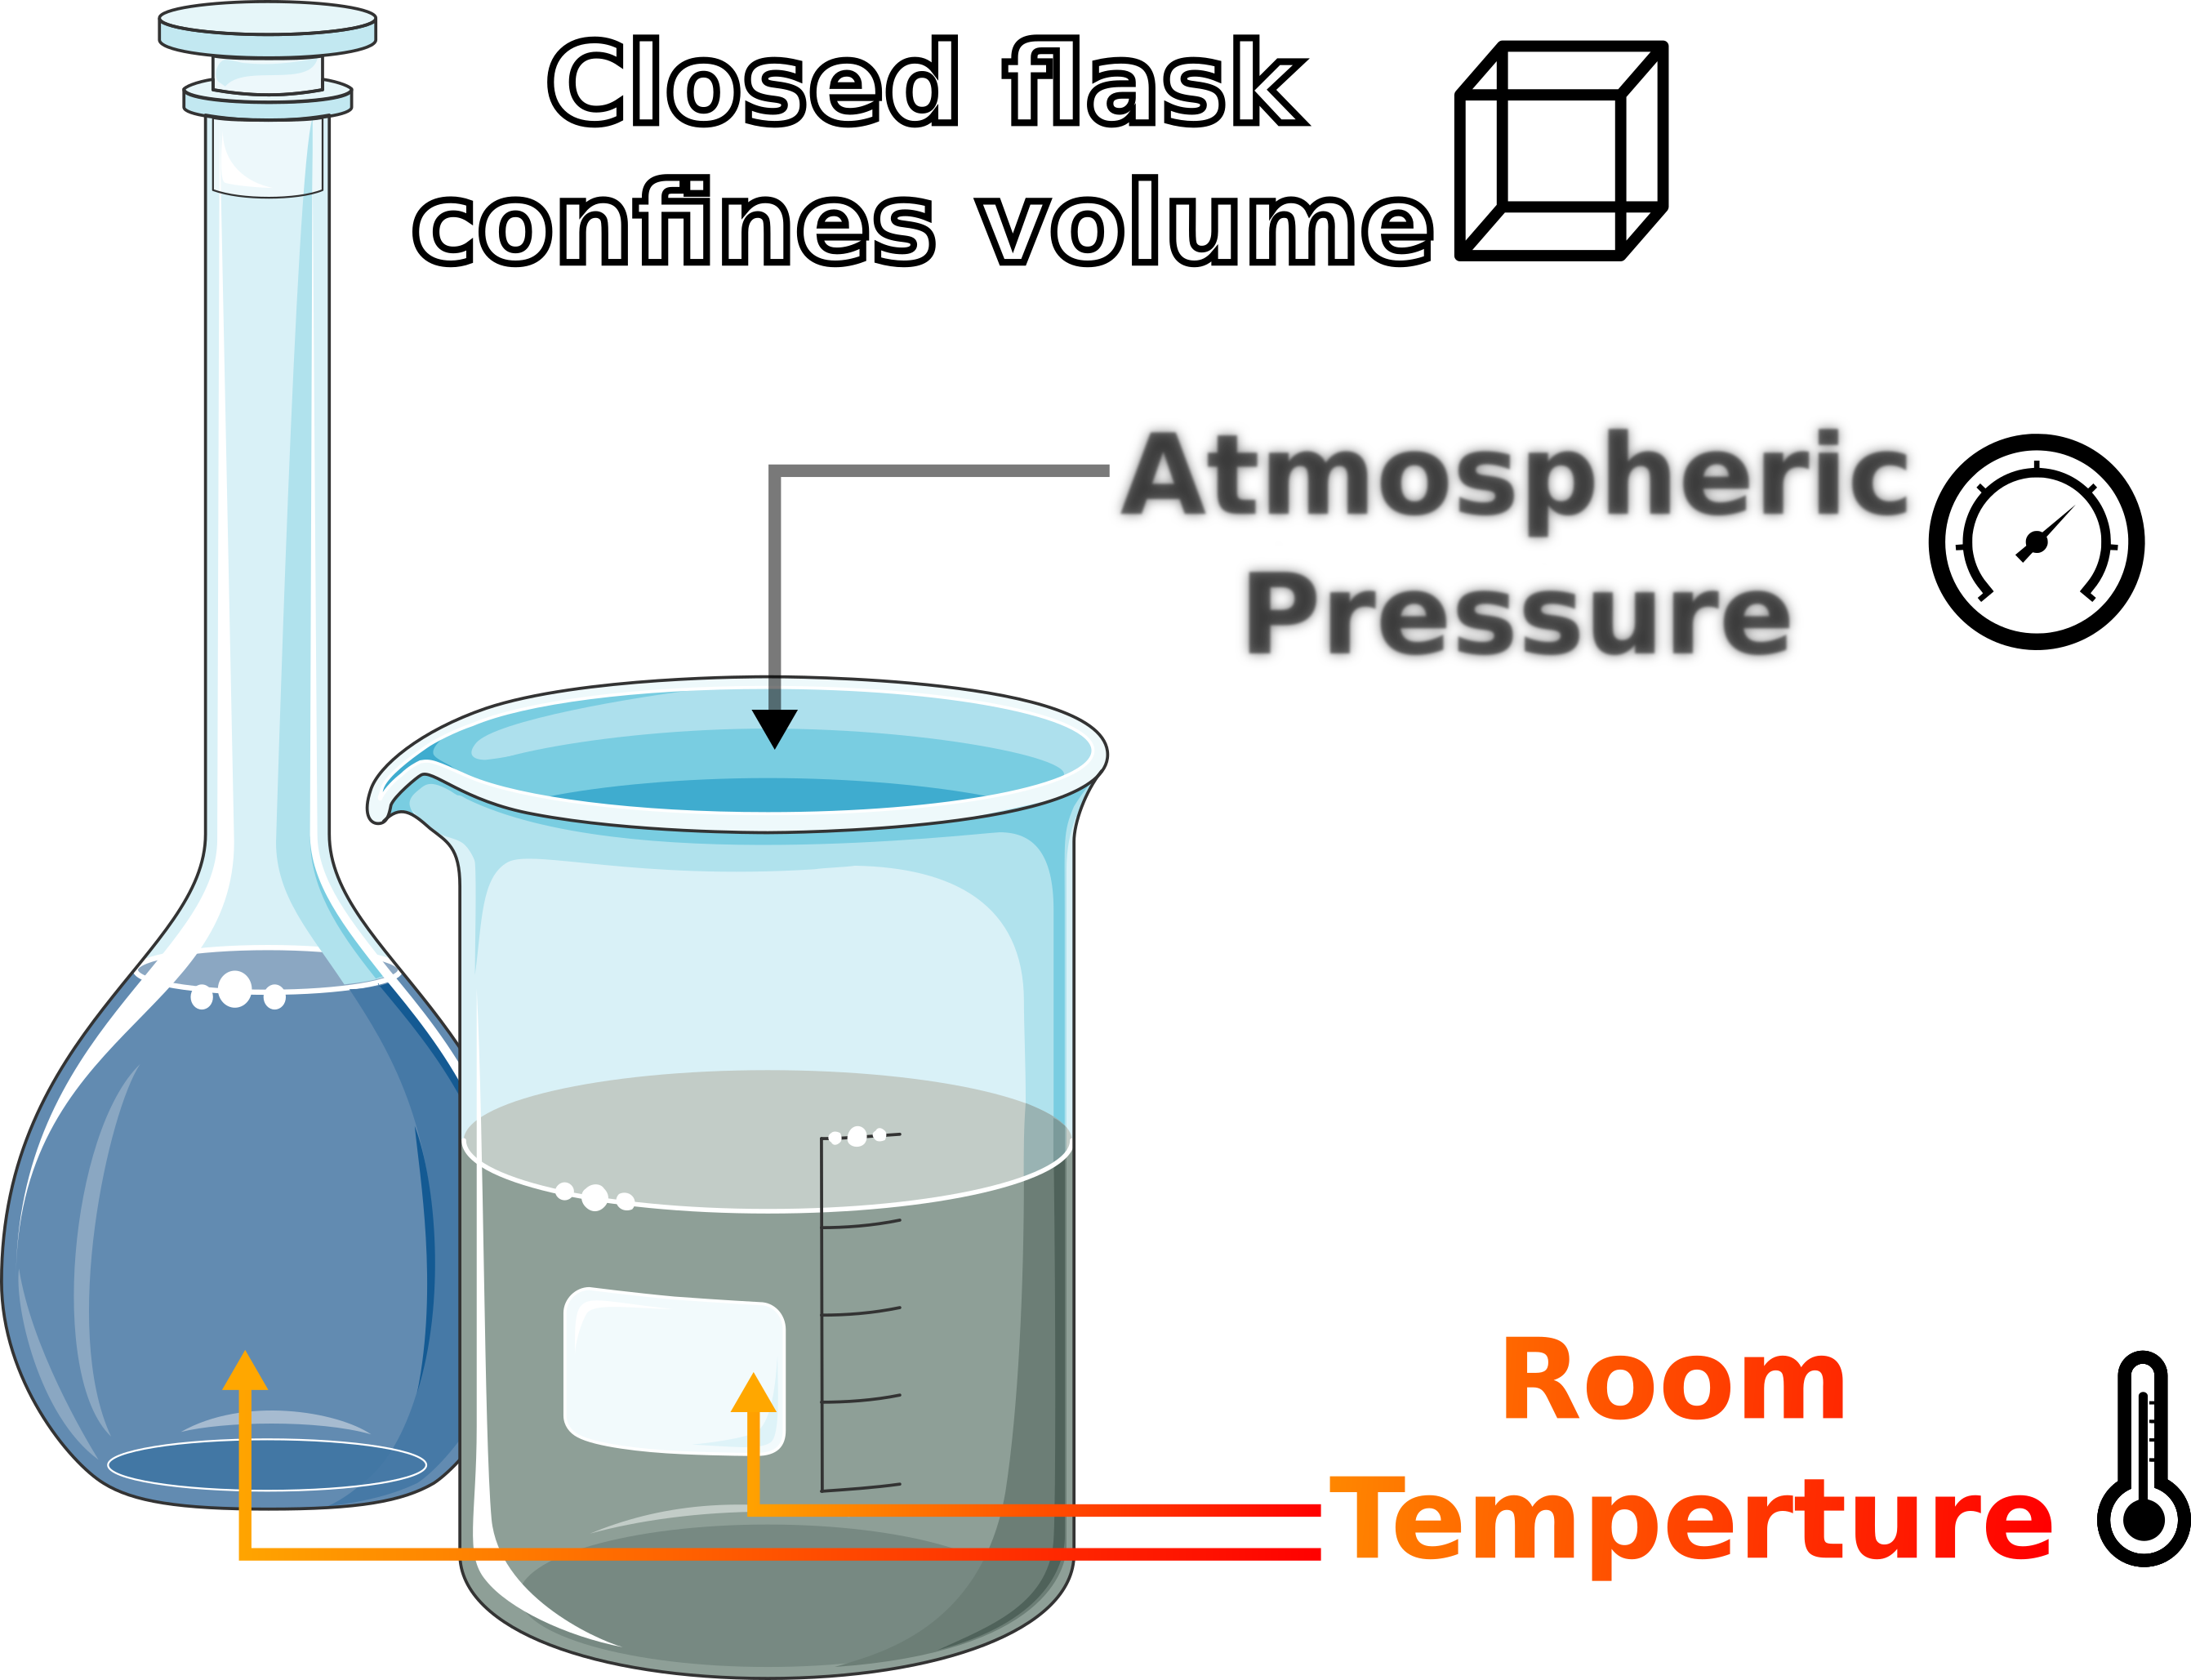
\includegraphics[width=0.48\textwidth]{figures/labsystems.png}
    \caption[Wet Labsystem Ensembles]{The application of a thermodynamic ensemble (NVT, NPT) is required to mimic the physical conditions in the wet lab. High-accuracy algorithms for barostatting and thermostatting are crucial to yield realistic results from a molecular dynamics (MD) simulation. \url{smart.servier.com/} (CC-BY 3.0)}
    \label{fig:wetlabsystems}
\end{figure}


\subsection{Introduction}
% Aiming of the section
In \fref{sec:tcoupling}, the application of thermostats was introduced, i.e., simulations in the NVT ensemble that maintains a constant temperature. This exercise focuses on pressure coupling and the isothermal-isobaric ensemble. A barostat ensures constant pressure while letting the volume fluctuate. Since most laboratory experiments are performed under constant pressure and temperature, employing the isothermal-isobaric ensemble (NPT) to achieve realistic simulations is often reasonable, i.e., a thermostat and a barostat algorithm must be employed to amend Newton's equations of motion. Usage of the barostat only will result in a different thermodynamic ensemble.\\
This exercise is split into three subtasks. Firstly, a TIP3P water box is tested for two different barostats (Berendsen and Parrinello-Rahman) and a range of coupling parameters. The coupling parameter $\tau_\text{\tiny P}$ defines the barostat's stiffness towards the reference pressure, similar to the thermostat. A comparison to TIP3P's literature isothermal compressibility $\kappa_\text{T}$ shall be conducted, which depends on the volume fluctuations of the simulation. Secondly, two further water models shall be simulated within the NPT ensemble, and their $\kappa_\text{T}$ values shall be compared to experimental water. Thirdly, two further simulations must be conducted and analyzed for their energetic properties. The simulation setup differs only slightly. However, the results deviate significantly, and the user should find out why. This exercise aims to teach how pressure coupling works and how the water model and coupling constant influence the thermodynamic quantities. Furthermore, understanding thermodynamic ensembles and their relation to MD simulations is further clarified. After this exercise, users will have a proper overview of how pressure coupling is implemented and be able to explore further details independently. 


\subsection*{Theoretical Considerations}
Conceptually, pressure coupling uses the same approach as temperature coupling, where velocities are rescaled via coupling to a heat bath. However, a barostat algorithm rescales the positions instead of the velocities; thus, the volume, $V$, is no longer constant. Other than that, many principles are analogous to thermostatting. E.g., the instantaneous pressure $P(t)$, the ensemble average of the pressure $\langle P\rangle_\text{\tiny NPT}$ and the reference pressure $P_0$ have their pendants in the previous exercise. The instantaneous pressure can be calculated via the kinetic energy of the system and the so-called inner virial $W_\text{\tiny inner}$ that depends on the pairwise forces $F_{ij}$ acting on two particles $i$ and $j$.\cite{Clausius1870,Brenig1996}
\begin{align}
    P(t) &= \frac{2}{3V} \left(E_\text{\tiny kin}(t) - W_\text{\tiny inner}(t) \right) \\
    P(t) &= \frac{2}{3V} \left(E_\text{\tiny kin}(t) - \frac{1}{2}\sum_{i}^N\sum_{j>i}^{N-1} r_{ij}(t) \cdot F_{ij}(t)  \right)
\end{align}
The formula is known as the virial theorem. Similarly to the barostat, the ensemble average of the system pressure can be approximated by the time average of the instantaneous pressure, given sufficient sampling.\cite{Coudene2016}
\begin{align}
    \langle P\rangle_\text{\tiny NPT}  \approx \frac{1}{{t_1} - {t_0}}\int_{t_0}^{t_1} P(t) dt
\end{align}
The plentifulness of barostat algorithms is up to par with thermostatting, and all algorithms feature different characteristics, benefits, and drawbacks. However, to showcase the implementation of a barostat, the simple but popular Berendsen barostat will be presented in all brevity. In the case of pressure coupling, the box size and the positions are scaled with a scaling factor $\mu$ to alter the result of the virial as a pressure correction. The Berendsen algorithm introduces a pressure change via a virtual pressure bath proportional to the difference between the reference and instantaneous pressures.\cite{Berendsen1984}
\begin{align}
    \frac{dP}{dt} & = \frac{P_0 - P(t)}{\tau_\text{\tiny P}}
\end{align}
Analogously to temperature coupling, the user-specified constant $\tau_\text{\tiny P}$ defines how tight the pressure coupling is. It can be shown that this differential equation leads to a scaling factor $\mu$ that also depends on the isothermal compressibility $\kappa_\text{T}$.\cite{Berendsen1984}
\begin{align}
    \mu = \sqrt[3]{1 + \frac{\Delta t \kappa_\text{T}}{\tau_\text{\tiny P}} \left(P(t) - P_0\right)}
\end{align}
Even when $\kappa_\text{T}$ might be unknown, it can be estimated since its accuracy only affects $\tau_\text{\tiny P}$, which can be chosen by the user over a wide range of values. Once $\mu$ is calculated from the instantaneous pressure, it is applied to the unscaled system coordinates $r^\prime(t)$ after numeric integration and velocity rescaling in the case of thermostatting.\cite{Berendsen1984}
\begin{align}
    r(t+\Delta t) &= \mu \cdot r^\prime(t+\Delta t) \\
    V(t+\Delta t) &= \mu^3 \cdot V(t)
\end{align}
After rescaling, the updated coordinates are used to calculate the forces in the next step via \fref{eq:NewtonsEqOfMotion}. Even though pressure coupling retains the reference pressure very well on average, it can lead to substantial variations in the instantaneous pressure. The large fluctuations are due to steep pressure-volume isotherms for liquid systems, i.e., a subtle change in volume leads to a considerable change in pressure and vice versa.\cite{Landau1980}\\
The isothermal compressibility is thermodynamic quantity that relates applied pressure to response in volume. The formula \texttt{GROMACS} uses to calculate $\kappa_\text{T}$ comprises the volume fluctuations $\text{RMSD}(V)$, the temperature $T$, the Boltzmann constant $k_\text{B}$ and the average volume $\langle V \rangle$.\cite{Allen1990}
\begin{align}\label{eq:isothermalcomp}
    \kappa_\text{T} & = \frac{\text{MSD}(V)}{k_\text{B} T \langle V \rangle}
\end{align}


\subsection*{Setup and Simulations}


\subsubsection*{The Choice of the Coupling Constant Matters}
Two barostats and six different coupling constants shall be evaluated in this sub-task. The \texttt{MDP} files can be found in the online directory, with missing values for the $\tau_\text{\tiny P}$-option and the barostat in the NPT input files. The values to be screened are listed in \fref{tab:tauPvalues}. In the previous three exercises, the necessary input files were already provided in the online resource. In this exercise, the user needs to create the necessary \texttt{GRO} and \texttt{TOP} files. However, manually creating the two missing files is an optional sub-task. If time is limited, this task may be skipped by using \texttt{tip3pbox.gro} and \texttt{tip3p.top} from the previous exercise.\\
The command \code{gmx solvate} is a good starting point. This command offers a variety of options to solvate systems or create them from scratch. Since the command is quite versatile, reading the \texttt{GROMACS} documentation is recommended to figure out the crucial flags and options. Set the box dimensions to \qtyproduct[product-units = single]{2.504 x 2.504 x 2.504}{\cubic\nano\metre} and even though we use TIP3P water, spc216 needs to be specified for the \code{-cs} flag. In \texttt{GROMACS} spc216 is the standard 3-Point water model \texttt{GRO} file, also representing the coordinates of the TIP3P model and all other 3-point water models. The same rationale holds for 4-Point and 5-Point water models as well.\\
Unfortunately, \code{gmx solvate} regularly fails to squeeze the requested amount of solvent into the simulation box. Hence, the \code{-maxsol} flag should be set to \num{1} so that we can use the resulting one-water \texttt{GRO} file as input for \code{gmx insert-molecules}. This command fills a given box with the required number of water molecules (\num{523}), and unlike \code{gmx solvate}, it tries to meet the specifications as many times as given in \code{-try}. The generated single-water \texttt{GRO} file should be used for the \code{-ci} flag. Finally, \code{gmx pdb2gmx} creates the respective \texttt{TOP} file, herein with the TIP3P water model and the amber99SB-ILDN forcefield. An exemplary workflow for creating the aqueous system is shown below.\\
\begin{lstlisting}[language=bash]
gmx solvate -cs spc216 -box 2.504 2.504 2.504 -maxsol 1 -o tip3p.gro
gmx insert-molecules -ci tip3p.gro -box 2.504 2.504 2.504 -nmol 523 -try 10000 -o choice_tauP.gro
gmx pdb2gmx -f choice_tauP.gro -p choice_tauP.top -water tip3p -o trash.gro # UI prompted after execution
\end{lstlisting}
% Adjustments to tauP and the measurements
As a reminder, directories and naming conventions should be kept clean and consistent within projects. Thus, names should be kept as short as possible and as informative as necessary to maintain a good overview. The simulation sequence consists of minimization, followed by an NVT simulation, and then the NPT-Ensemble. The values for $\tau_\text{\tiny P}$ can be found in the following table. For certain $\tau_\text{\tiny P}$ values, adjusting the \code{-maxwarn} flag of \code{gmx grompp} might be necessary.
\begin{table}[H]
    \centering
    \caption{Values for the coupling constants are to be screened by the user for both barostats.}
    \label{tab:tauPvalues}
    \begin{tabular}{l | r r r r r r}
        \toprule
        $\tau_\text{\tiny P}$/\SI{}{\per\pico\second} & 0.05 & 0.1 & 0.5 & 1 & 5 & 10 \\
        \bottomrule
    \end{tabular}
\end{table}
For the Parrinello-Rahman barostat and the $\tau_\text{\tiny P}$ values \SI{0.05}{\per\pico\second} and \SI{0.1}{\per\pico\second} the additional option \texttt{nstpcouple = 1} must be inserted in the respective \texttt{MDP} file (position in the file is arbitrary). For each NPT simulation, plot the Volume $V$ and Pressure $P$ against time and calculate the variance of the volume $\sigma_\text{V}^2$ throughout the simulation. Concerning the plots, the first few frames may be excluded if they do not represent an equilibrated system using \code{gmx energy -b <FRAME>}. The volume fluctuations $\sigma_\text{V}^2$ are linked to the isothermal compressibility $\kappa_\text{T}$ to be calculated for each $\tau_\text{\tiny P}$ as well. Tabulate the various values of $\sigma_\text{V}^2$ and $\kappa_\text{T}$ and feature the plots in the report. Additionally, discuss which of the $\tau_\text{\tiny P}$ and barostats delivers results comparable to the literature value of $\kappa_\text{T}^\text{\tiny TIP3P}=\SI{6.3e-5}{\per\bar}$ and why others may fail.\cite{Bernetti2020} The command \code{gmx energy} is highly recommended to conduct the result collection. The command is analogous to the one used last week to obtain the isochoric heat capacity. The \textit{energetic} properties that need to be selected from the interactive menu can be deduced from \fref{eq:isothermalcomp}.
\begin{lstlisting}[language=bash]
gmx energy -f <ENERGYFILE> -o <OUTPUTFILE> -fluct_props -nmol <NUMBER>
\end{lstlisting}


\subsubsection*{Influence of the Water Model on the Isothermal Compressibility}
In this task, two water models should be simulated to investigate the influence of different water models on $\kappa_\text{T}$. Optimally, the experimental value $\kappa_\text{T}^\text{\tiny exp} = \SI{4.52e-5}{\per\bar}$ for \SI{298.15}{\kelvin} is retained from the simulation runs.\cite{Linse2021} The water models in question are the SPC/E and TIP4P water models. This time, the simulation procedure includes an energy minimization, an NVT- and NPT-equilibration, concluded by the pre-production and production run. It is common practice to use the Berendsen thermostat and barostat for the NVT- and NPT-equilibrations since it is robust and computationally inexpensive. The pre-production and production runs are usually simulated using the Nose-Hoover and Parrinello-Rahman algorithms for high-fidelity production data. The pre-production run facilitates the system adjusting itself to the enhanced algorithms. As shown in the previous exercise, some algorithms sample a certain ensemble more reliably, which implies that the system has to adapt to certain physical changes. The analysis should not include the transition time necessary for this adaptation since it does not represent the thermodynamic equilibrium. The data for result computation should stem only from the fully equilibrated production run.\\
In order to save time, \code{nsteps} in the \texttt{MDP} files can be adjusted based on the MD runs from the first task. Simulations should be long enough to collect sufficient data to compute results, but not longer. The \code{nsteps} option may be decreased to save time.\\
All necessary \texttt{MDP} files are given or can be repurposed, and the \texttt{TOP} and \texttt{GRO} files can be obtained in the aforementioned fashion. \texttt{SPC/E} is a three-site water model, and \texttt{TIP4P} is a four-site water model. Thus, the correct option for the \code{-cs} flag must be ensured.
\begin{lstlisting}[language=bash]
gmx solvate [...] | gmx insert-molecules [...] | gmx pdb2gmx [...] # Procedure of obtaining GRO and TOP file
\end{lstlisting}
Once the simulations have finished, \code{gmx energy} is recommended to evaluate which of the water models performs better concerning $\kappa_\text{T}$.


\subsubsection*{Simulation Behaviour for Large $\tau_\text{\tiny T}$ Values}
% context to the task and properties that are affected
In the preceding tasks, strengths and weaknesses between algorithms were uncovered, parameter choices for $\tau_\text{\tiny P}$ were examined, and the feasibility of different water models. Thus, the pressure coupling setup was the only aspect of interest. This last task serves as a reminder that a simulation consists of a delicate interplay of various algorithms and their settings.\\
Therefore, two simulation setups shall be compared with each other. One features a relatively tight pressure coupling and a high $\tau_\text{\tiny T}$ value, corresponding to infrequent corrections to the temperature. Meanwhile, the $\tau_\text{\tiny T}$ and $\tau_\text{\tiny P}$ values of the other setup can be considered standard.\\
% simulation setup and expected outputs
The system itself is the same as in the second task. Therefore, the only differences lie in the \texttt{MDP} files deposited in the online repository. Said files, \texttt{standard.mdp} and \texttt{non\_standard.mdp}, should be used to simulate the NVT-equilibrated SPC/E system from the second task. Once the simulation is done, use \code{gmx energy} to calculate and plot the kinetic energy $E_\text{kin}$, the potential energy $E_\text{pot}$, the density $\rho$, the enthalpy $H$ and the total energy $E_\text{tot}$ of the two simulations.\\
% Task descrription
The plots should be included in the report, and differences in their appearances should be discussed. An explanation for the observed behavior and a simulation-related way to test this explanation should also be given.

\newpage

\section{Exercise 5: The Significance of Accurately Calculated Long-Range Interactions}\label{sec:longrangeIA}
\begin{Checklists}
    \begin{checklist}{Tasks for the Fifth Exercise}
    \textbf{Finish these tasks and write a short report about your findings.}
    \begin{itemize}
		\item From the SPC/E water simulation, compare the first two peak positions of the RDF for all six different potential-modifiers with the experimental values.
		\item Include RDF plots for all the methods with a qualitative and quantitative comparison to \fref{fig:dnardf}.
		\item Include time-resolved plots and averages of the RMSDs for all the different methods with a brief discussion.
		\item Analyse all results regarding quality and performance and try to determine a best-practice method. Include the timings in this discussion.
	\end{itemize} 
    \end{checklist}
\end{Checklists}
\begin{figure}[H]
    \centering
    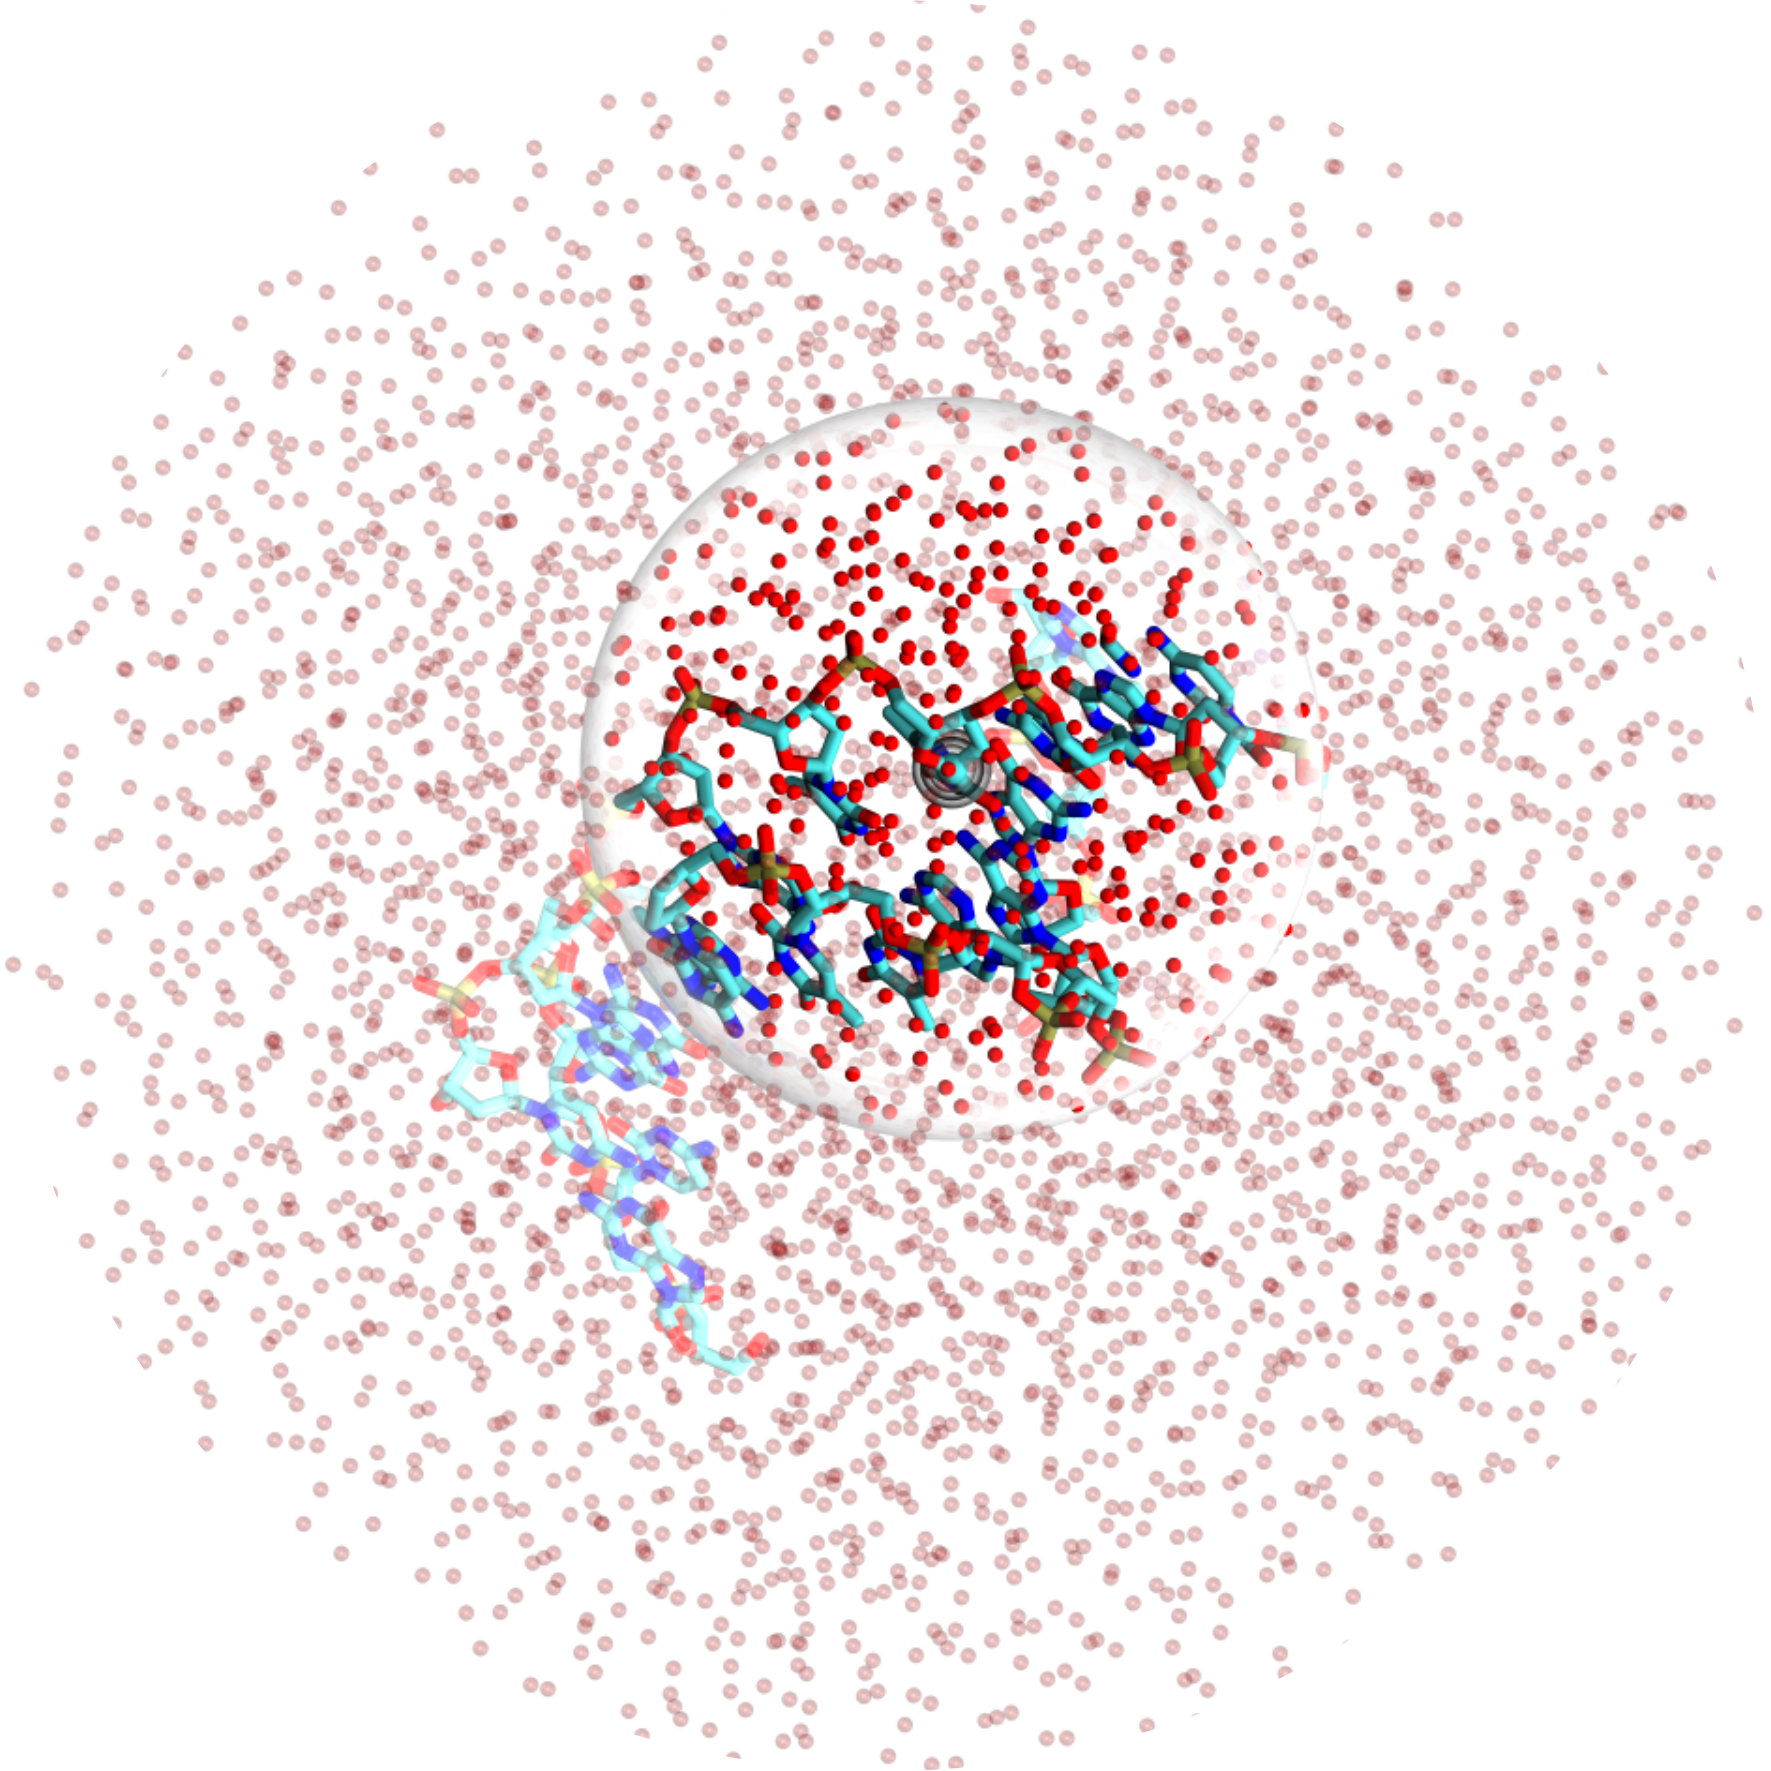
\includegraphics[width=0.48\textwidth]{figures/VMD_rendered_cover_art.png}
    \caption{Simplified visualization of the cutoff radius. Every opaque particle falls within the (enlarged) central particle's cutoff, signified by the \textit{forcefield bubble}. Non-bonded interactions with (transparent) particles outside this bubble would be omitted in a corresponding molecular dynamics (MD) simulation.}
    \label{fig:VMD_rendered_cover_art}
\end{figure}


\subsection*{Theoretical Considerations}
The most demanding task for molecular dynamics software is calculating pairwise additive interactions, i.e., the charge-charge interaction and the London-dispersion interactions modeled most often via the Coulomb and Lennard-Jones potential. The Lennard-Jones potential was already introduced in \fref{sec:ForceField}. It consists of a repulsive and an attractive term. Two constants are required to parameterize the potential, usually called $\sigma$ and $\varepsilon$. Physically, $\sigma$ is associated with the excluded volume of the respective atom, thus its radius, while $\varepsilon$ is the maximum potential well depth.\cite{LennardJones1924}
\begin{align}
    U_{\varepsilon,\sigma}(r_{mn})= 4 \varepsilon \left [ {\left (\dfrac{\sigma}{r_{mn}} \right )}^{12}-{\left (\dfrac{\sigma}{r_{mn}} \right )}^{6} \right]
\end{align}
The Coulomb potential is proportional to the Coulomb constant, the charge product of the two interacting particles and scales with $r^{-1}$. The coulomb constant consists of two other constants, $\pi$ and the electric permittivity in the vacuum $\epsilon_0$.\cite{Griffiths2017}
\begin{align}
    U_\text{\tiny C}(r_{mn}) = \frac{q_m q_n}{4 \pi \epsilon_0 r_{mn}}
\end{align}
Since both of these potentials are pairwise additive, a double sum over all particles has to be calculated; therefore, the computational cost scales with $N^2$ where $N$ is the number of particles in the system. Thus, the non-bonded interactions account for most of the computational time and are the main subject of algorithmic optimization. Both forces, resulting from the Coulomb potential $U_\text{C}$ and Lennard-Jones potential $U_{\varepsilon,\sigma}$, converge to $0$ for infinite interatomic distances, and the Lennard-Jones converges faster than the Coulomb potential. Therefore, a simple option is to introduce a cutoff radius $r_\text{\tiny cutoff}$ beyond which the interactions are set to zero. Such a cutoff can have various forms and implementations. Either the potential energy function is abruptly set to zero after the cutoff distance, or a so-called shifting or switching function is applied, smoothly bridging the potential function to zero at the cutoff distance. The latter two options yield relatively small errors for the quickly converging Lennard-Jones potential (converges with $r^{-6}$ towards zero). However, significant distortions must be expected for the slowly converging coulomb potential (converges with $r^{-1}$ towards zero).\cite{Norberg2000}\\
More complex methods based on the Ewald summation have emerged to treat long-range electrostatics more effectively. Ewald summation was initially invented to estimate the potential energy of crystal lattices\cite{Ewald1921}, and several techniques have branched out to approximate the electrostatic interactions in molecular dynamics simulations, such as P3M\cite{Hockney2021}, PME\cite{Darden1993} and SPME\cite{Essmann1995}.\\
For the illustration of long-range electrostatic treatment, the Ewald-based methods will be omitted since their mathematical framework is beyond the scope of this document. Instead, two potential shifting functions are showcased to make the topic tangible to the user. The two functions $S_1$ and $S_2$ ensure that the electrostatic interactions cross zero when $r_\text{\tiny cutoff}$ is reached.\cite{Prevost1990}
\begin{align} \label{eq:truncationPotSwitch}
S_{1}(r_{mn}) = 
\begin{cases}
  1 - 2 \frac{r}{r_\text{\tiny cutoff}} + \left( \frac{r}{r_\text{\tiny cutoff}} \right)^2  &  (r < r_\text{\tiny cutoff})\\
  0 & (r \geq r_\text{\tiny cutoff}) \\
\end{cases}\\
S_{2}(r_{mn}) = 
\begin{cases}
  1 - 2 \left(\frac{r}{r_\text{\tiny cutoff}}\right)^2 + \left( \frac{r}{r_\text{\tiny cutoff}} \right)^4  &  (r < r_\text{\tiny cutoff})\\
  0 & (r \geq r_\text{\tiny cutoff}) \\
\end{cases}
\end{align}
The modified potentials $U^\prime$ are the product of the coulomb potential with its shifting function, and the resulting force is the negative derivative with respect to position.
\begin{align}
    U^\prime(r_{mn}) &= U_\text{\tiny C}(r_{mn}) \cdot S(r_{mn}) \\
    F^\prime &= -\frac{\partial U^\prime}{\partial r_{mn}}
\end{align}
Although the truncation largely decreases the computational cost, the modified potentials and their resulting forces deviate substantially from the original. The differences between the potentials are visualized in \fref{fig:PotentialShifting}. Both modified potentials underestimate the energy contribution by a large margin, and for the forces, the $S_1$ function consistently underestimates the coulomb force, while the $S_2$ function overestimates short-ranged interactions. 
\begin{figure}
    \centering
    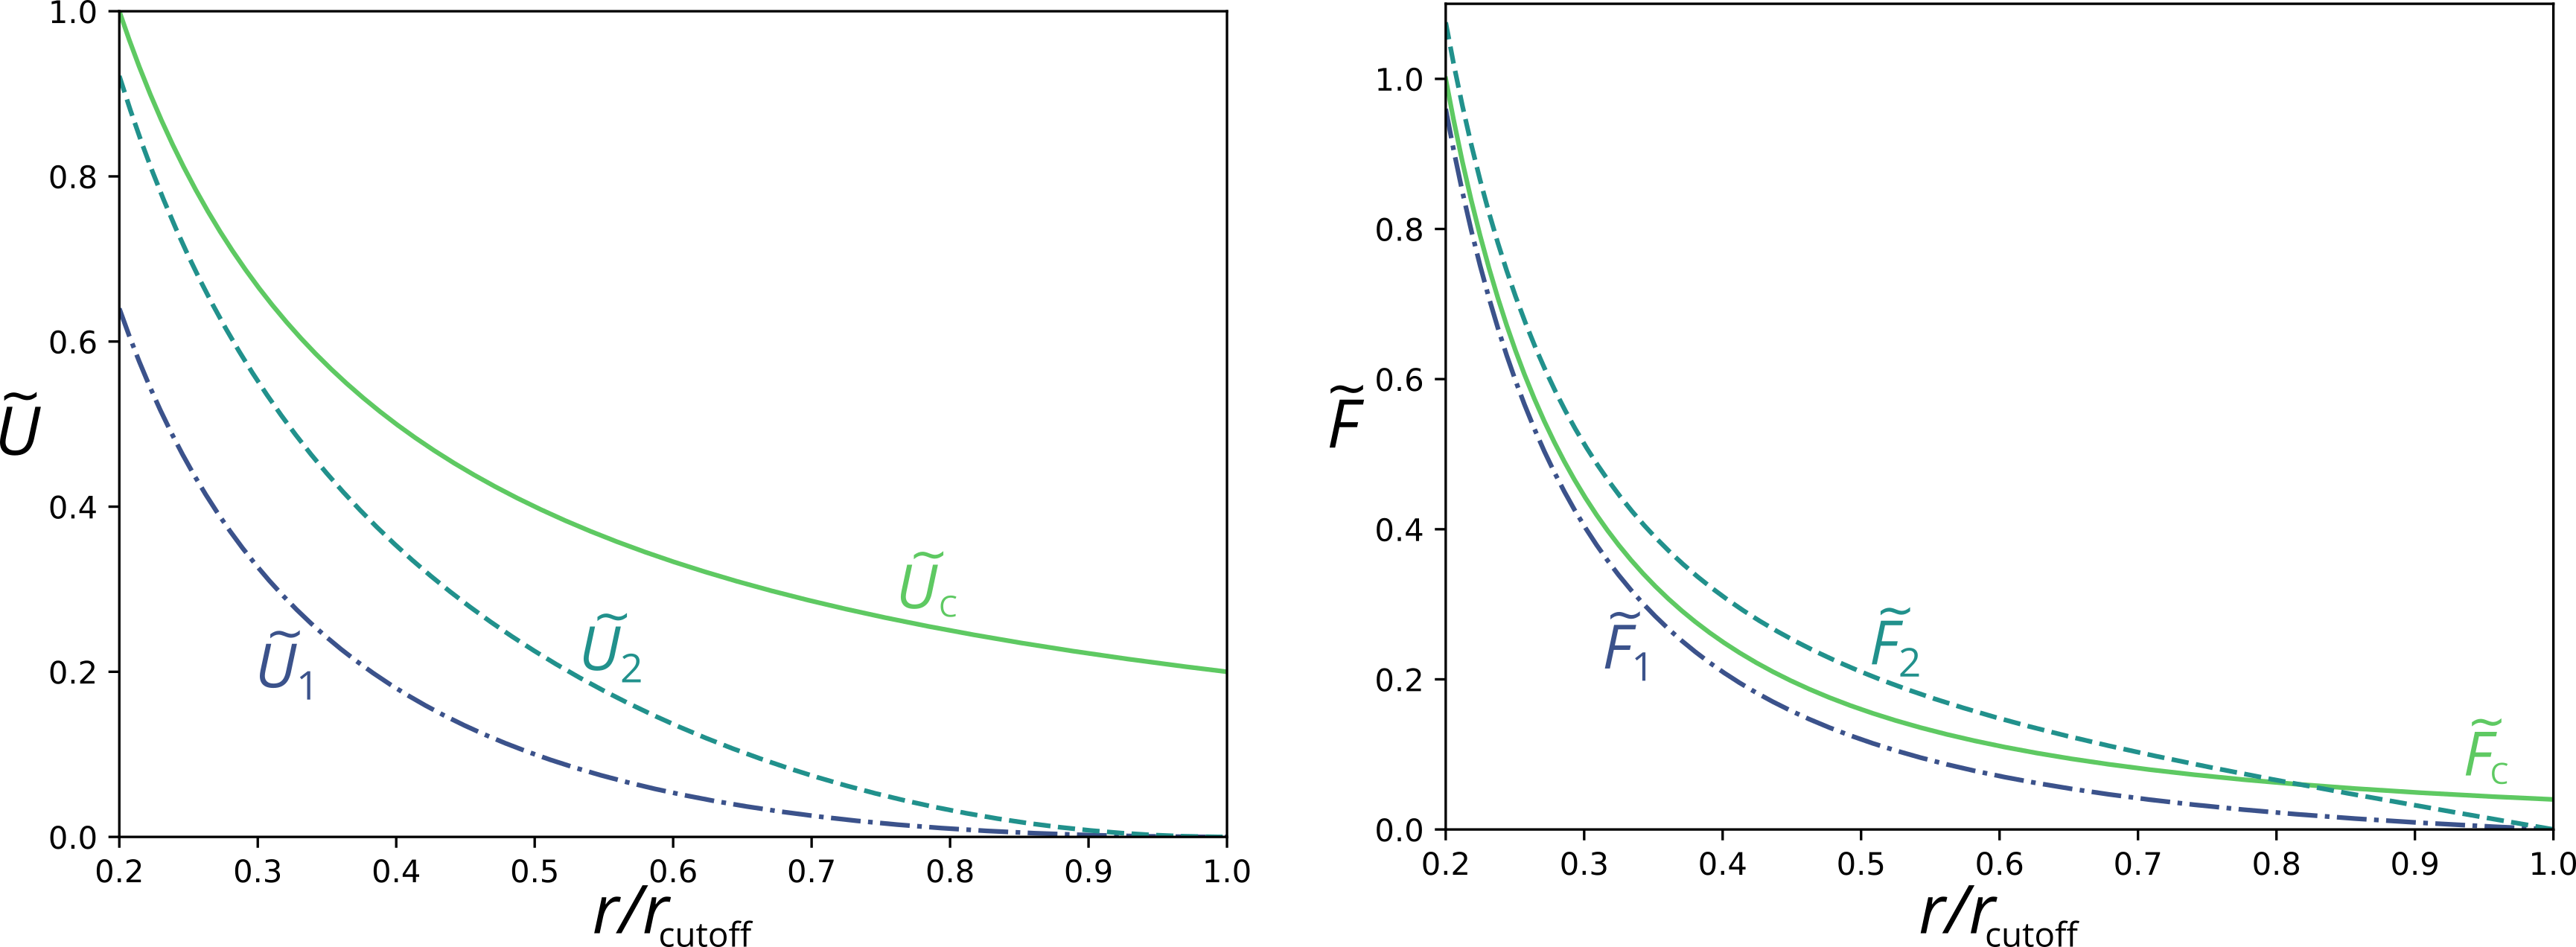
\includegraphics[width=0.48\textwidth]{figures/PotentialShifting.png}
    \caption{The reduced potential energy functions $\widetilde{U}$ and forces $\widetilde{F}$ are plotted to visualize the different behavior of the two shifting functions compared to the unfettered coulomb potential. Adapted from Prevost et al.\cite{Prevost1990}}
    \label{fig:PotentialShifting}
\end{figure}
Furthermore, the radial distribution function (RDF) shall be introduced which is a measure for quantitatively testing the effect of long-range electrostatics. The RDF between particle group A and B ($g_\text{AB}(r)$) describes the structure of (isotropic) liquids and liquid mixtures. It works by counting the particles of type B at a certain distance from a central particle of type A. The abundance of B as a function of the distance reveals information about their intermolecular interactions and could be used to calculate several thermodynamic properties. To calculate $g_\text{\tiny AB}(r)$ the average particle density of particle type B for a distance $r$, $\langle \rho_\text{\tiny B}(r)\rangle$, is divided by the bulk density $\langle \rho_\text{\tiny B} \rangle_\text{\tiny bulk}$,
\begin{align} \label{eq:gab_simple}
    g_\text{\tiny AB}(r) & = \frac{\langle \rho_\text{\tiny B}(r)\rangle}{\langle \rho_\text{\tiny B} \rangle_\text{\tiny bulk}} \quad .
\end{align}
The bulk density for B is usually calculated for the complete simulation box, hence dividing $N_\text{\tiny B}$ by the box volume $V_\text{\tiny Box}$. For a continuous distance, the average particle density B around A can be written in terms of the Kronecker-delta $\delta (...)$ of the particle distance $r_{mn}$ and the surface area of the sphere,
\begin{align} \label{eq:rhoABr}
    \langle \rho_\text{\tiny B}(r) \rangle & = \frac{1}{N_\text{\tiny A}} \sum_{i \in A}^{N_\text{\tiny A}} \sum_{j \in B}^{N_\text{\tiny B}} \frac{\delta\left(r_{mn},r\right)}{4 \pi r^2} \quad ,
\end{align}
where $\delta(r_{mn},r)=1$ if $r_{mn} = r$ and $\delta(r_{mn},r)=0$ otherwise.
The expression becomes slightly more complicated for the non-continuous case natural to computational methods. Firstly, spherical shells with a thickness of $\Delta r$ are considered instead of a sphere's surface, which effectively turns $g_\text{\tiny AB}(r)$ into a histogram depending on $n$ bins $g_\text{\tiny AB}(n)$ of bin width $\Delta r$. Let $r_n$ and $r_{n+1}$ be the lower and upper border of the $n$-th bin. Then, this histogram function can be calculated by augmenting \fref{eq:rhoABr} with the Iverson bracket notation and the formula for a spherical shell,
\begin{align} \label{eq:rhoABn}
    \langle \rho_\text{\tiny B}(n) \rangle & = \frac{1}{N_\text{\tiny A}} \sum_{i \in A}^{N_\text{\tiny A}} \sum_{j \in B}^{N_\text{\tiny B}} \frac{\left[ r_n < r_{mn} < r_{n+1} \right]}{\frac{4}{3} \pi (r_{n+1}^3 - r_n^3)} \quad .
\end{align}
This expression can be simplified by assuming that each shell is very thin, hence $\Delta r \ll r_n$. Given \texttt{GROMACS}' default bin width of \SI{2}{\pico\meter}, this assumption is satisfied, resulting in the final expression of the discretized radial distribution function,
\begin{align} \label{eq:gABn}
    g_\text{\tiny AB}(n) & = \frac{1}{N_\text{\tiny A} \langle \rho_\text{\tiny B} \rangle \text{\tiny bulk} } \sum_{i \in A}^{N_\text{\tiny A}} \sum_{j \in B}^{N_\text{\tiny B}} \frac{\left[ r_n < r_{mn} < r_{n+1} \right]}{4\pi r_n^2 \Delta r} \quad .
\end{align}
Notice that A and B can also be of the same particle type, which helps investigate the structure of pure liquids like pure water, mainly since the RDF can be obtained from scattering experiments and MD simulations. A direct comparison of the plot appearance can hint towards the forcefield quality of the water model and the methods as well. 
\begin{figure}[H]
    \centering
    \includegraphics[width=0.48\textwidth]{figures/spceRDFoo.png}
    \caption[RDF-Schematic and RDF of SPCE Water]{Left: Schematic on how the RDF is calculated. Right: The RDF of water oxygens of pure SPC water calculated from Simulation.\cite{Berendsen1981}}
    \label{fig:rdf_spcwater}
\end{figure}


\subsection*{Setup and Simulations}
\subsubsection*{Water Structure Under the Influence of Different Electrostatic Interaction Schemes}
% Motivation
The finite size of the simulation box and the periodic image limits the range of long-range interactions. Additionally, the computational time depends largely on the number of atom pairs, for which non-bonded interactions have to be calculated. Introducing a potential-modifier using a cutoff distance $r_\text{cutoff}$ to truncate non-bonded interactions remedies these issues. On the other hand, a realistic physical description must be maintained as well as possible, leading to various algorithms that mingle with this trade-off. In this exercise, the user explores some of these potential modifiers, analyses them for their strengths and weaknesses, and presents one solution as their personal recommendation.\\
% The algorithms
Herein, algorithms for plain cutoff, potential shift modifiers, and the Particle-Mesh-Ewald (PME) method are investigated. The two former methods rely on cutoff truncation to simplify the calculation of electrostatic interactions. For these methods, a metric must be defined that tells \texttt{GROMACS} when to shift the potential and truncate the non-bonded interactions. The PME method, on the other hand, makes use of lattice Ewald summations (implemented using Fast Fourier Transforms) to simplify the calculation of long range electrostatic interactions in a periodic system. Its use requires the specification of several \texttt{MDP} options beyond this document's scope. The prepared \texttt{MDP} files can be downloaded from the online repository.\\
% The Simulations
As usual, the system must be set up using \texttt{GROMACS}' tools. The edges of the cubic box should be \SI{4}{\nano\meter}, and the SPC/E water model is supposed to be used with the amber99SB-ILDN forcefield. The \texttt{MDP} files for the equilibrations can be downloaded (EM, NVT, and NPT). The system can be equilibrated once, followed by the pre-production and production run for each long-range electrostatics treatment. In this exercise, six different modifiers are tested: PME, potential-shift with \SI{8}{\angstrom} and \SI{12}{\angstrom} cutoff, and the truncation method with \SI{8}{\angstrom}, \SI{12}{\angstrom} and \SI{18}{\angstrom} cutoff. The time benchmarks should be extracted from the \texttt{LOG} file (outputted automatically) to be included in the report. Usually, there are two different run time measurements: the wall time and the core time. The wall time measures the real-world time that elapses during the MD run, and the core time refers to the time spent by all processors to execute every command. The latter is more important in this task and should be compared for the different electrostatic interaction schemes, preferably in a table with a brief discussion.\\
A quantitative comparison can be conducted utilizing RDF peak positions. In \fref{fig:rdf_spcwater}, the peak locations correspond to solvation shells of water molecules. Therefore, the first peak corresponds to the location of the first, very distinct solvation layer. The second peak corresponds to the second less pronounced solvation shell. The simulation quality can be accessed by comparison with the experimental peak positions. Therefore, the report should include the timings and positions of each method's first two RDF peaks and a quantitative comparison. Experimental values for comparing $r_1$ and $r_2$ were measured by Skinner et al.\cite{Skinner2014}. They found $r_1$ at \SI{2.79983}{\angstrom} and $r_2$ at \SI{4.5149}{\angstrom} for a temperature of \SI{300}{K}. Notice that the RDF is calculated for the water oxygen atoms, not the whole molecules. For completing this task, \code{gmx rdf} is highly recommended. The \texttt{GROMCAS} command line reference should be consulted since this command is quite versatile (see \url{manual.gromacs.org/documentation/2018/user-guide/cmdline.html}). As a hint, the \code{-ref} and \code{-sel} flags and specify the atom names given in the \texttt{GRO} file.


\subsubsection*{A-DNA and B-DNA Simulations with Different Electrostatic Interaction Schemes}
% Introduction
After the investigation of pure water, the effects of different methods to calculate electrostatic interactions are probed for complex bio-molecules. Herein, A-DNA and B-DNA are simulated, both stable conformations of Watson-Crick-base-paired DNA. However, B-DNA has been proven to be more stable. Furthermore, DNA is a highly charged molecule with many anionic oxygen atoms in the phosphate backbone. Thus, it is expected that the treatment of long-range electrostatic interactions has a vast impact on DNA stability and structure.\\
\begin{figure}[H]
    \begin{subfigure}[c]{0.5\textwidth}
        \centering
        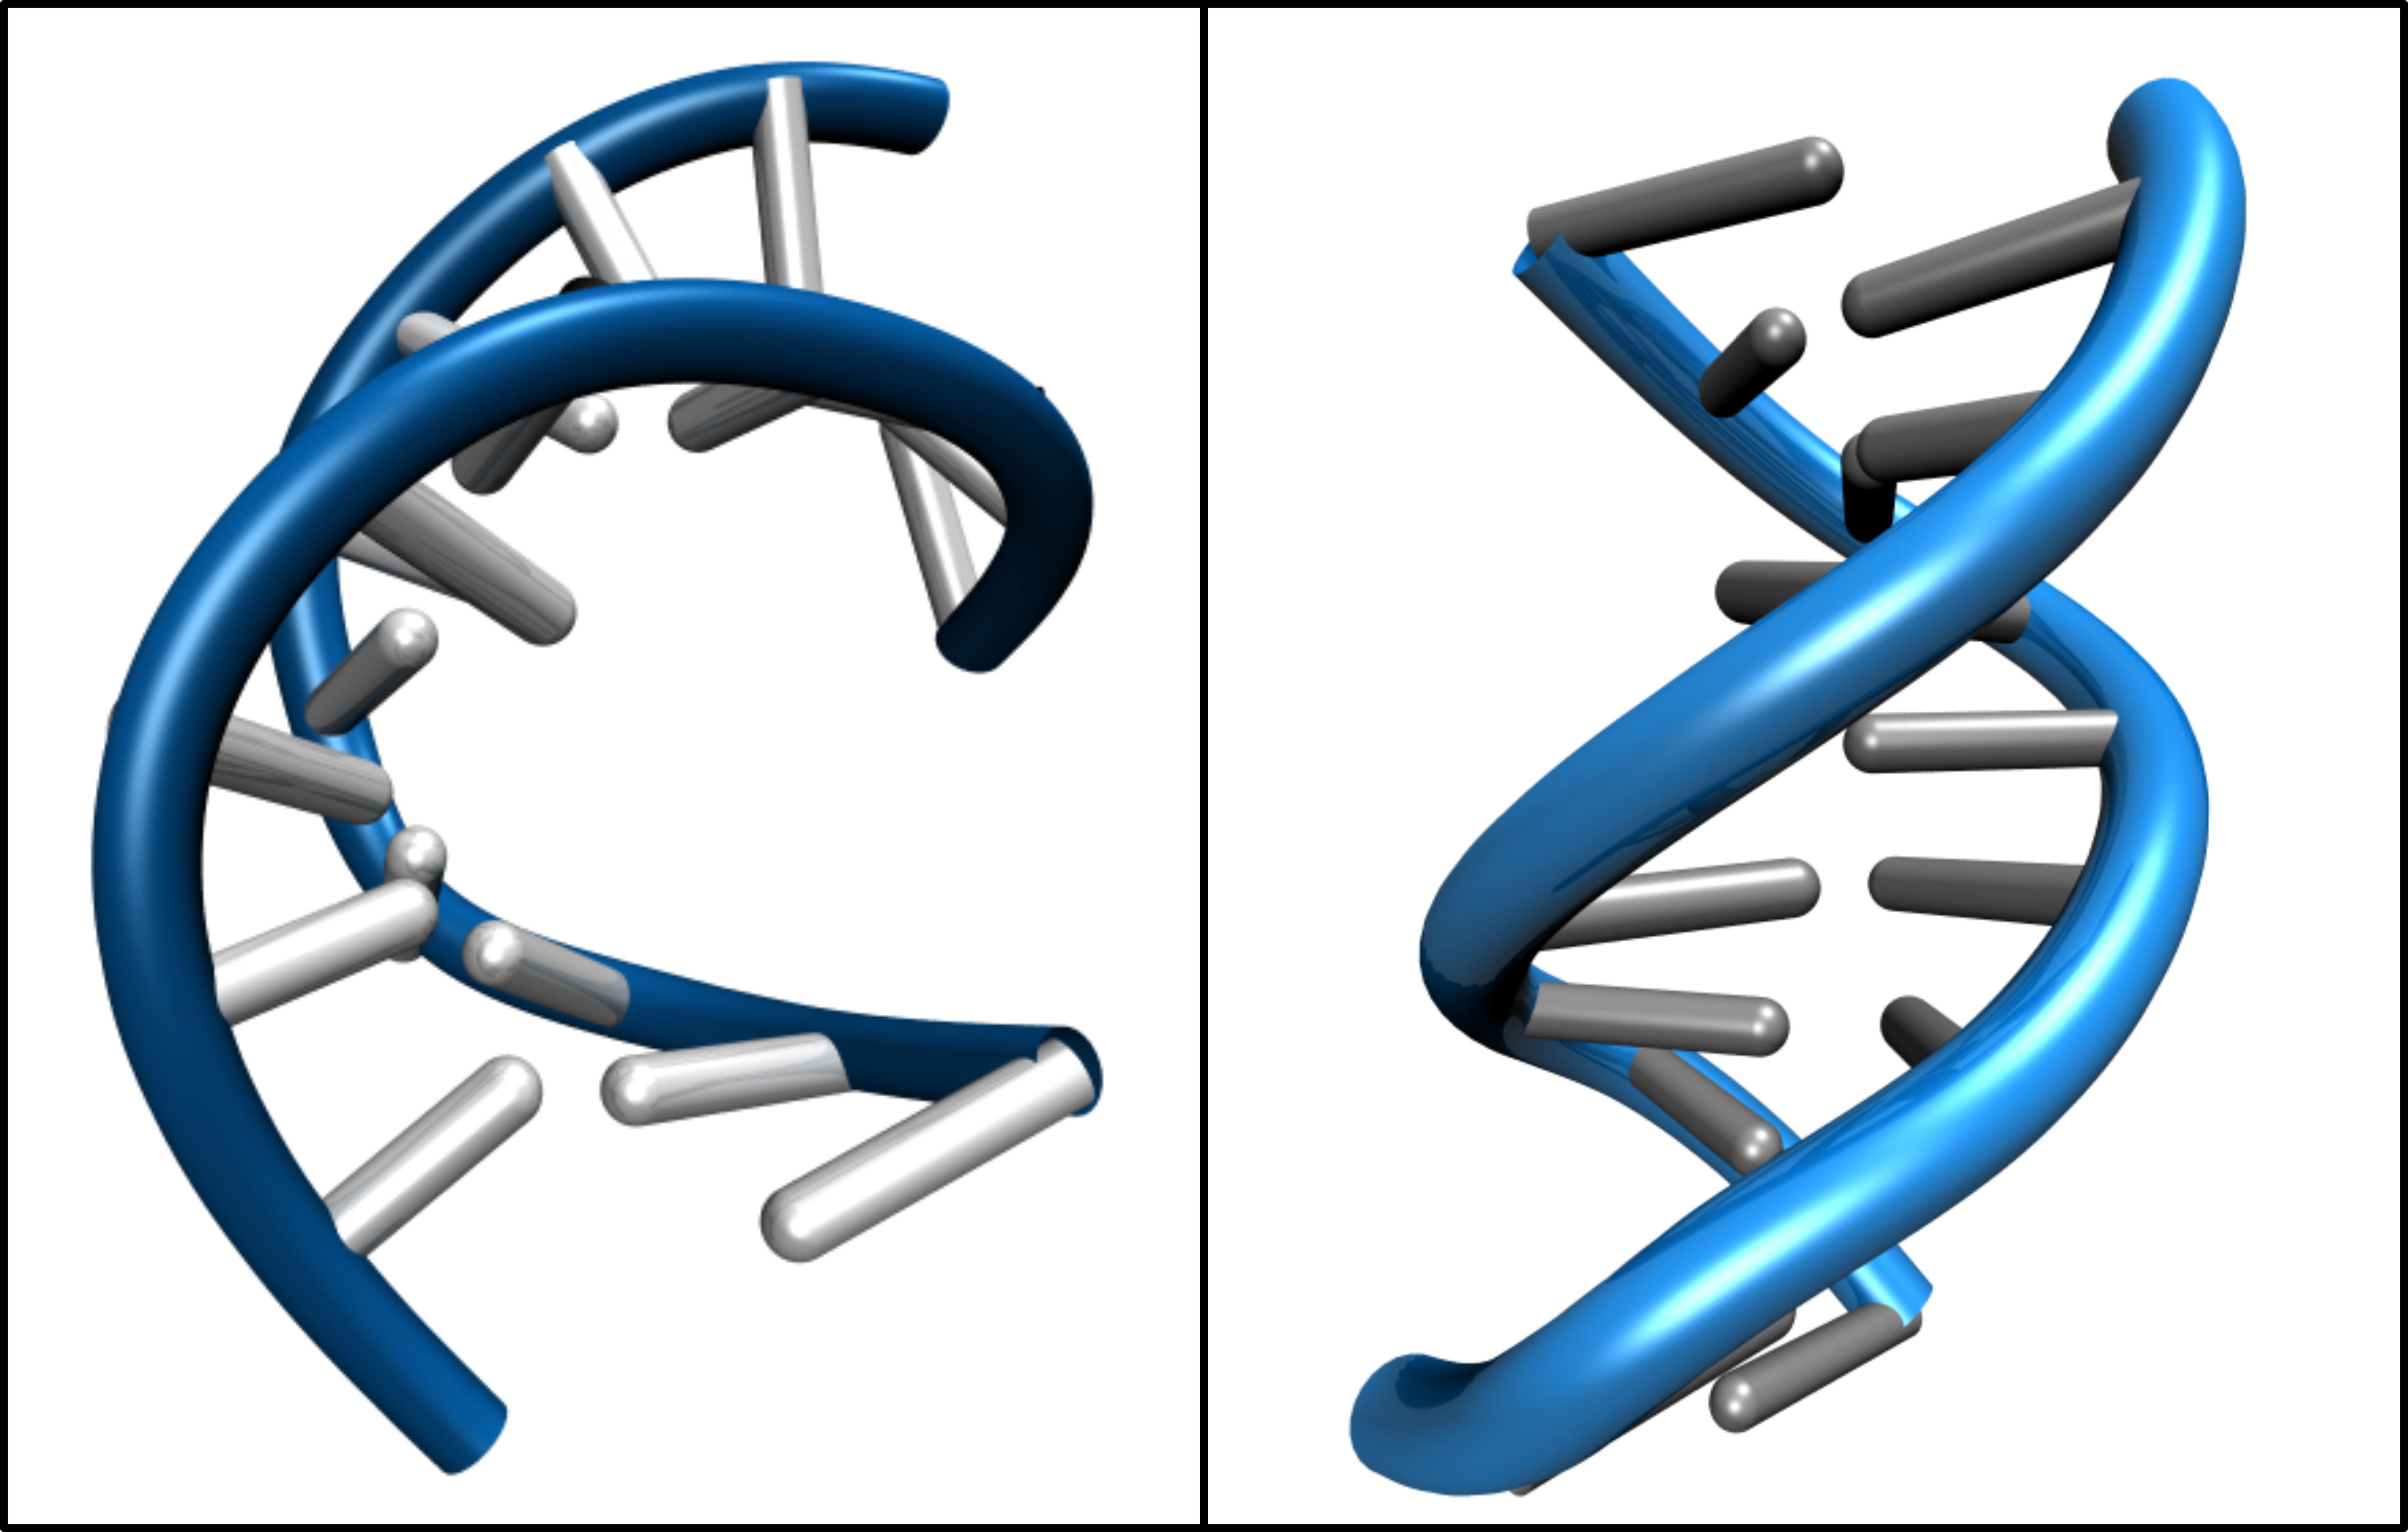
\includegraphics[height=55mm]{figures/a_b_dna.png}
        \caption{}
        \label{fig:abdna}
    \end{subfigure}
    \begin{subfigure}[c]{0.5\textwidth}
        \centering
        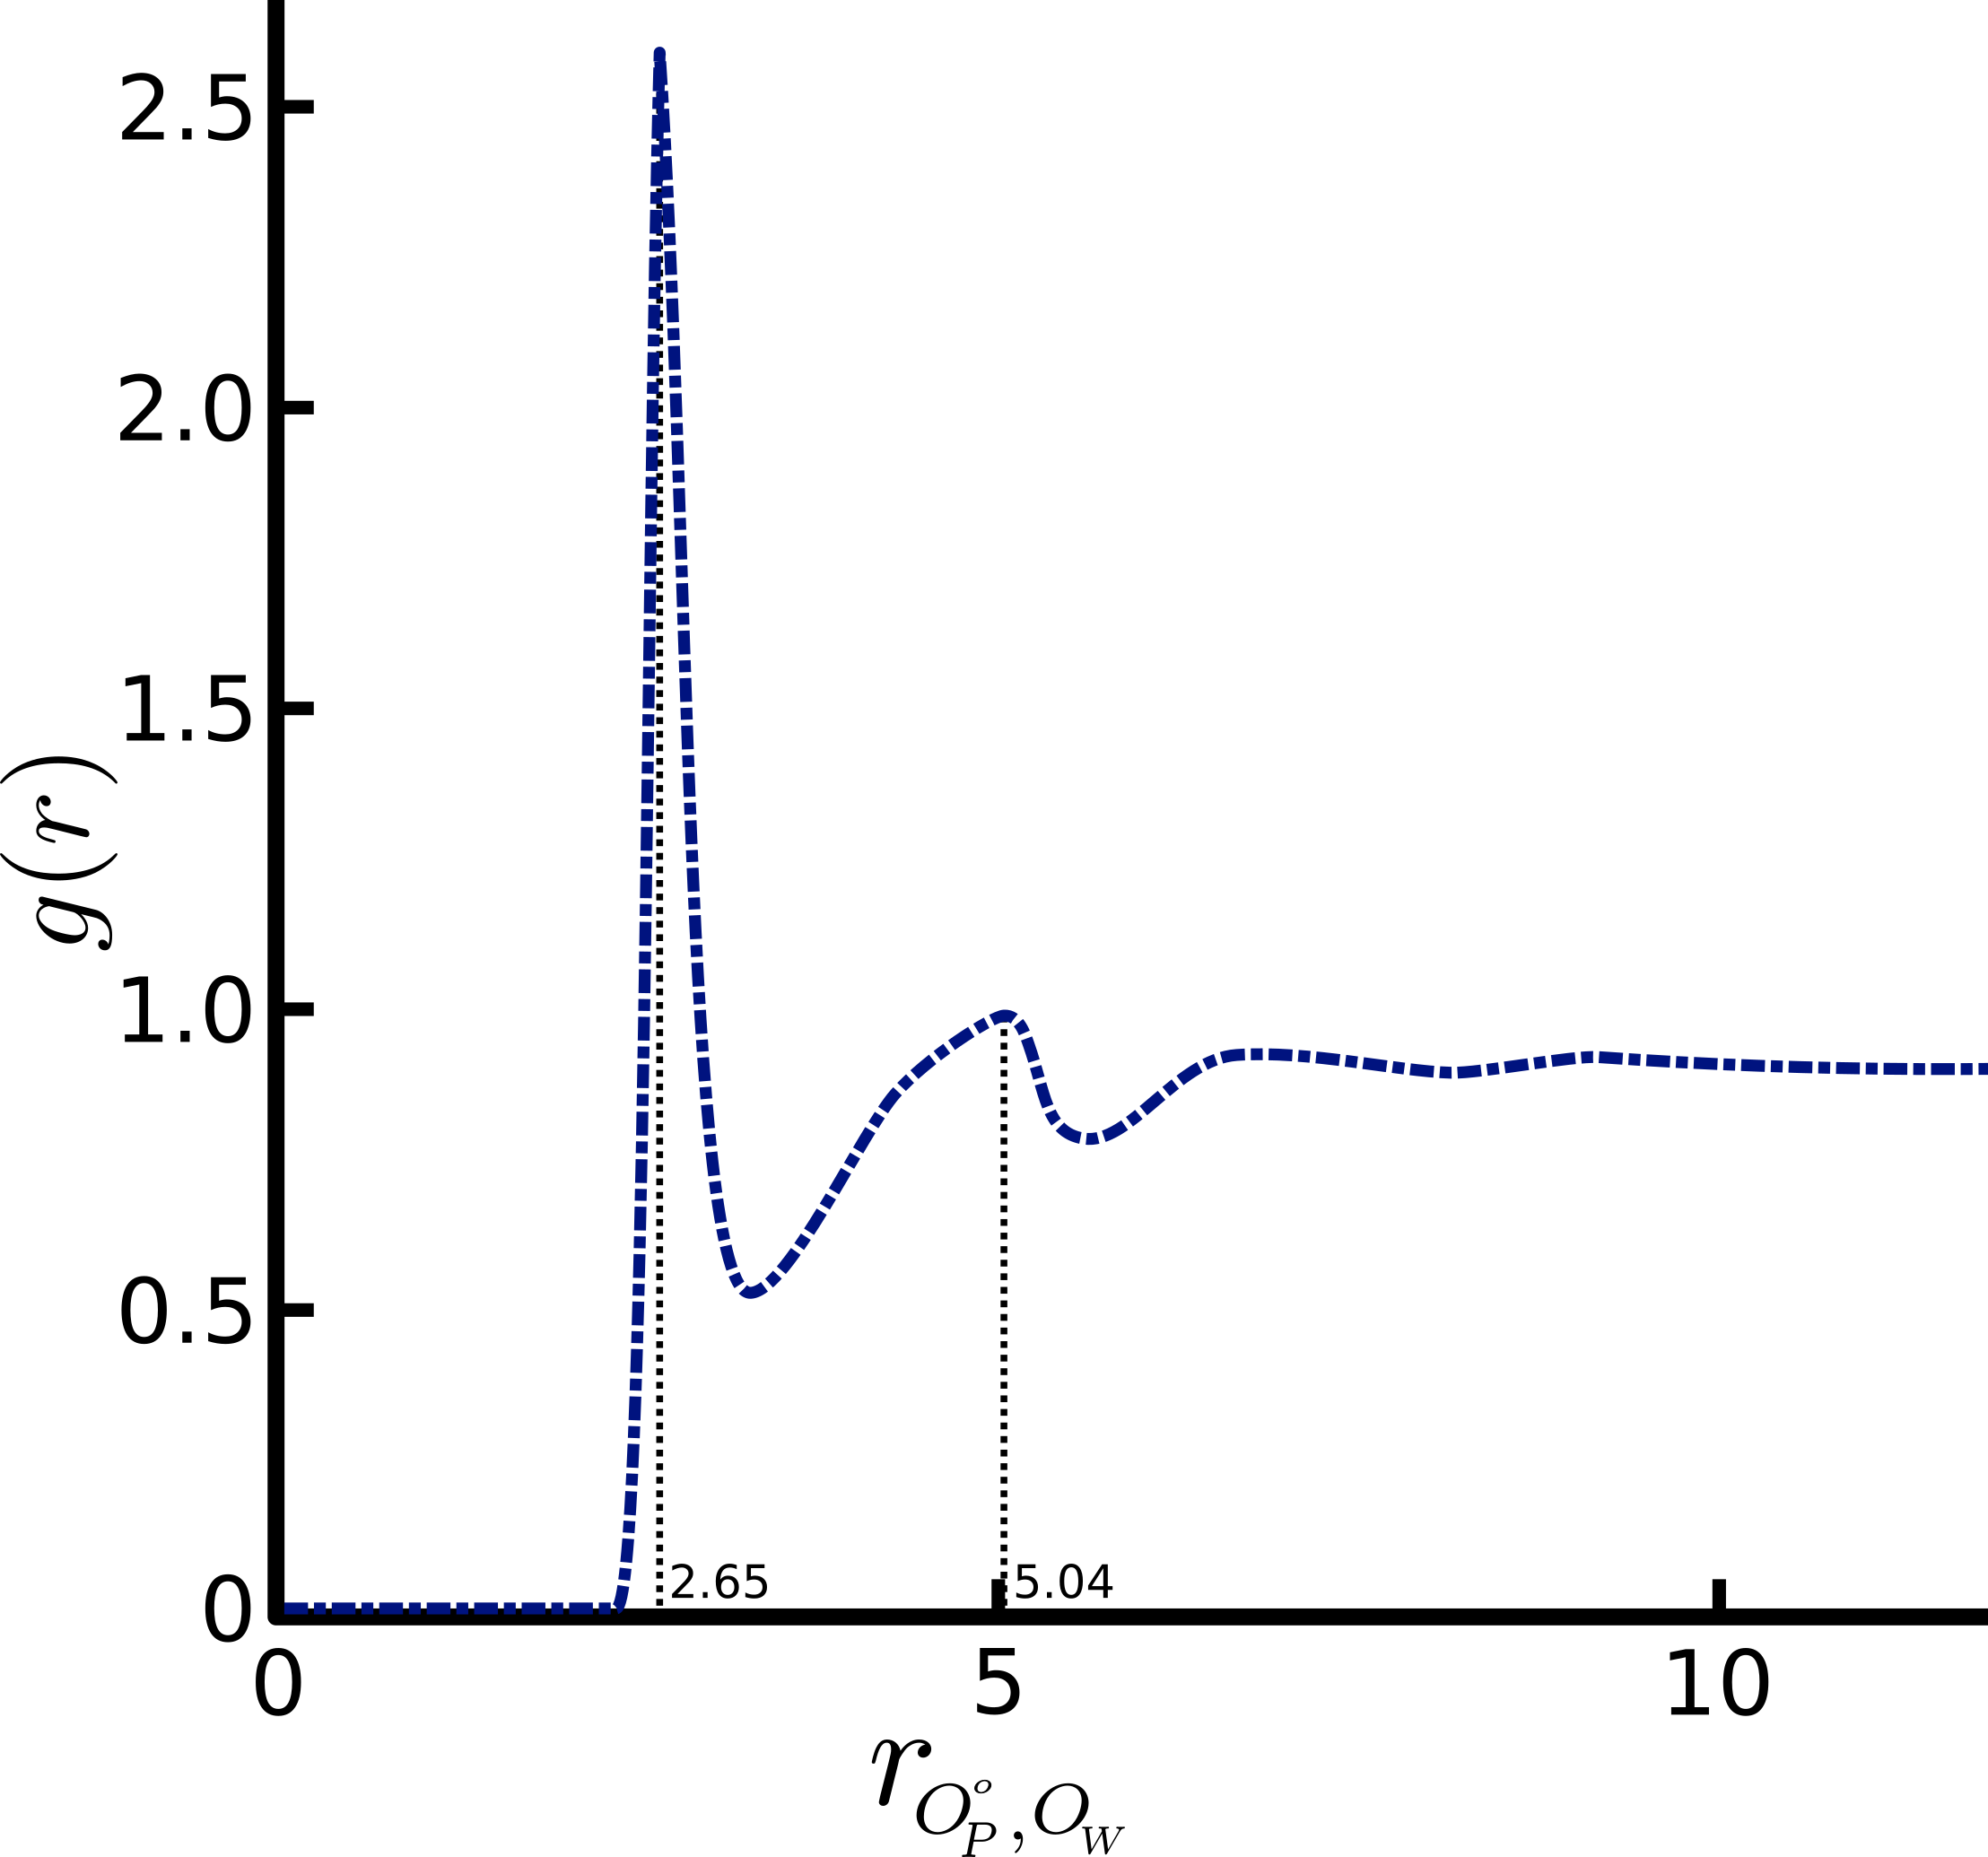
\includegraphics[height=55mm]{figures/Ref_DNA_RDF.png}
        \caption{}
        \label{fig:dnardf}
    \end{subfigure}
    \caption[DNA Conformations and Published RDF]{a) A-DNA and B-DNA conformations (visualized by VMD). B-DNA exhibits the classical helix shape. b) RDF calculated by Jaiswal et al.\cite{Jaiswal2018} between the uncharged phosphate oxygen atoms and the water oxygen atoms. The peak positions are indicated on the x-axis.}
\end{figure}
% Simulation Setup and files.
The files necessary for the simulations can be downloaded from the online repository. The setup consists of six electrostatic interaction schemes (same as in the prior task). Two PDB files, pictured in \fref{fig:abdna}, contain the coordinates of the DNA molecules. The usual \texttt{GROMACS} programs are used to generate a solvated simulation box from the PDB files.
\begin{lstlisting}[language=bash]
gmx pdb2gmx [...]  # Use AMBER99SB-ILDN and SPC/E water; also specify flag: -ignh
gmx solvate [...]  # solvates the simulation box; Use cubic box with edge length 5 nm
gmx grompp [...]   # just to generate tpr file for gmx genion
gmx genion [...]   # replaces water with ions; just neutralise the DNA
\end{lstlisting}
After the system generation, the same \texttt{MDP} files as in the first section should be used to equilibrate the system. The electrostatic interaction schemes become important only for the pre-production and production run, from which the data is collected for analysis.\\
% Analysis
The information of interest consists of the RMSD, the RDF, and the timings of the production run for each method since the calculation of non-bonded interactions is the major bottleneck of the performance. The timings are readily collected from the \texttt{LOG} file. In order to extract the other information from the trajectories, they need to be augmented first. Augmentation in the sense that the DNA molecules should be centered in the simulation box since they can be broken across periodic boundaries, which messes up the measurements. The \texttt{GROMACS} tool that can manipulate trajectories is called \code{gmx trjconv}, which is used in combination with an index file  (\texttt{NDX}) to target a non-standard atom group. Herein, the non-standard group consists of one ssDNA strand, which is necessary because centering the DNA dimer can position each DNA strand on opposing periodic boundaries. \texttt{GROMACS} has its own tool to generate \texttt{NDX} files, fittingly called \code{gmx make\_ndx}, which offers a command-line interface. Within this prompt, the user has to pick the correct atoms resembling the desired index group, e.g. 'a 1-315', followed by saving the new index group by typing \keystroke{q} {\small+} \keystroke{enter}. Since the website information for \code{gmx trjconv} is quite confusing, the correct options for the command are given below.
\begin{lstlisting}[language=bash]
gmx trjconv -f <PROD-TRAJ>.xtc -s <PROD-STRUC>.tpr -center -n <INDEX>.ndx -pbc mol -o <WHOLE-TRAJ>.xtc
\end{lstlisting}
After execution, \code{gmx trjconv} prompts the user for which group to center (the ssDNA) and which group to output (the whole system). The RMSD of the trajectory is to be calculated in reference to its first frame, a.k.a. the last frame of the pre-production run. To make sure that the reference frame is not split across periodic boundaries, \code{gmx trjconv} needs to be called for \texttt{<PRE-GRO>.gro} as well.
\begin{lstlisting}[language=bash]
gmx trjconv -f <PRE-GRO>.gro -s <PRE-STRUC>.tpr -center -n <INDEX>.ndx -pbc mol -o <WHOLE-GRO>.gro
\end{lstlisting}
The resulting trajectory can then be used to calculate each system's RDF and RMSD curves (The RDF can also be calculated with the non-augmented trajectory). Herein, the RDF should be determined between the neutral phosphate oxygens and the water oxygens (see \fref{fig:dnardf} for plot appearance and reference peak positions). Thus, the plot appearances should be compared qualitatively, whereas the peak locations should be compared quantitatively. The command \code{gmx rdf} is recommended to fulfill this task.\\
Regarding the RMSD, two measurements are of utmost importance: the time-resolved RMSD and the average RMSD of the production run. The reference structure that is always needed to calculate an RMSD is the prepared \code{<WHOLE-GRO>.gro} file and needs to be specified in the \code{-s} flag of \code{gmx rms}. The report should include RMSD plots of all the different methods and a comparison with \fref{fig:DNARMSD}, assessing which cutoff scheme produces realistic RMSD curves. Furthermore, a brief discussion of the average RMSDs for each method should be included.\\
Eventually, all results from the DNA and the water simulations should be used to select the simulation setup that appears most suitable to calculate electrostatic interactions, with a brief explanation. While timing information is crucial, the quality of the results is to be ranked as more important in this evaluation.
\begin{figure}[H]
    \centering
    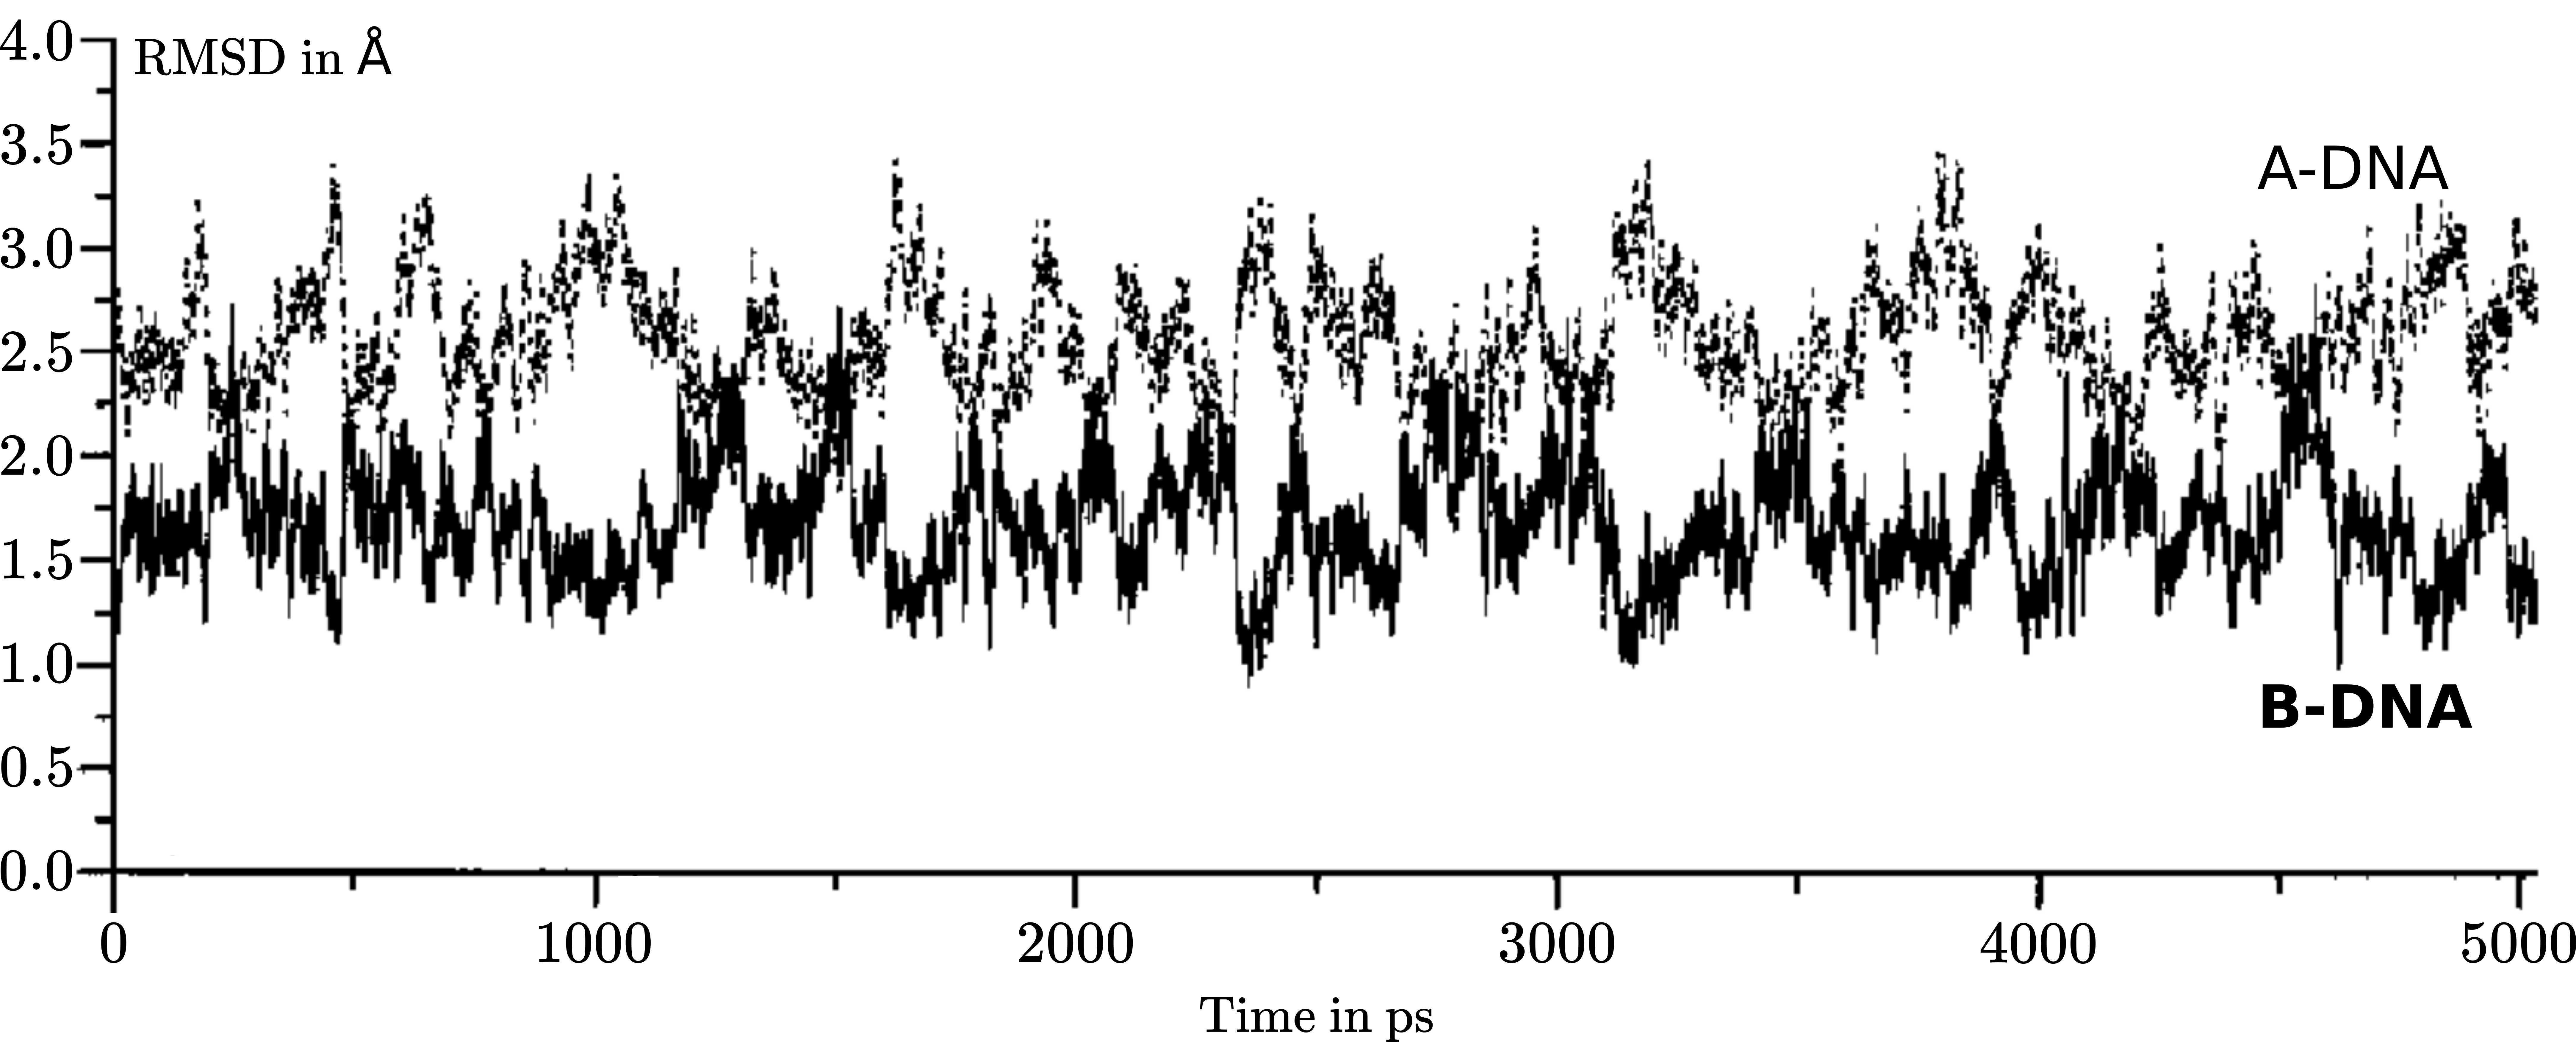
\includegraphics[width=0.45\textwidth]{figures/DNA_RMSD.png}
    \caption[Exemplary time resolved RMSD]{Exemplary time resolved RMSD. Modified from Norberg et Nilsson.\cite{Norberg2000} B-DNA is slightly more stable, which results in an overall lower RMSD. However, the fluctuations seem comparable to those seen in the visual inspection.}
    \label{fig:DNARMSD}
\end{figure}

\newpage

\section{Exercise 6: Calculation of the Solvation Free Energy of Methane Using the MBAR Method}\label{sec:freeEnerSolv}
\begin{Checklists}
    \begin{checklist}{Tasks for the Sixth Exercise}
    \textbf{Finish these tasks and write a short report about your findings.}
    \begin{itemize}
		\item Complete the missing parts in the two bash scripts \code{run\_lambda\_simulations.sh} and \code{generate\_mdp\_files.sh} and include your code suggestions in the report (as a screenshot or similar).
		\item Use \code{gmx bar} to generate your \code{bar.xvg} and \code{barint.xvg} and include the plots in your report with a brief discussion. 
		\item Discuss your result for $\Delta G_{solv}$ and compare it to the one in the literature.
	\end{itemize} 
    \end{checklist}
\end{Checklists}


\subsection*{Acknowledgement}
This exercise was inspired by a tutorial offered by Justin Lemkul.\cite{Lemkul2019}


\subsection*{Introduction}
In contrast to prior exercises that focused on exploring different algorithms, this exercise centers on a specific application: calculating free energy changes. Free energy calculations are critically important in computational biophysics because they quantify various biologically relevant processes, such as stability alterations due to point mutations, small ligand binding, and solvation free energy of organic molecules.\cite{Mobley2006} Setting up and analyzing these simulations involves numerous choices experienced users must carefully select.\cite{Christ2009}\\
The system of interest in this exercise is an aqueous system with a single methane molecule. The goal is to calculate the solvation free energy, $\Delta G_\text{solv}$, for the methane molecule. This exercise will also convey an understanding of such calculations' physical and mathematical aspects and the computational framework provided by \texttt{GROMACS}. While an in-depth exploration of free energy calculations is beyond the scope of this document, additional sources can be consulted for further information.\cite{Pohorille2010,Villa2002,Bennett1976}\\
The property to be calculated, $\Delta G_\text{solv}$, was reported in 2003 by Shirts et al. They found a value of \SI{2.42}{\kilo\calorie\per\mole} for the OPLS-AA forcefield.\cite{Shirts_2003} By following the steps described below, it should be possible to replicate their results with reasonably good agreement.\\ 


\subsection*{Theoretical Considerations}
% Solvation Free Energy: A Theoretical Background
Solvation free energy, $\Delta G_\text{solv}$, also known as the Gibbs free energy of solvation, is a fundamental concept in physical chemistry. It quantifies the free energy change when a solute dissolves in a solvent, usually under standard conditions (pressure of \SI{1}{\bar}, temperature of \SI{298.15}{\kelvin}, and concentration of \SI{1}{\mole\per\liter}). 
The process of solvation entails changing the whole chemical environment of the solute. Thus, the solute might rearrange because its intra-molecular interactions adjust to the solvent contacts that suddenly present themselves. Exposed hydrophobic entities would aggregate within each other, while buried hydrophilic entities might become solvent-accessible. Especially for complex molecules and solvents (it does not have to be water), there is no way to intuitively estimate the solvation free energy given the multitude of (competing) enthalpic and entropic driving factors. Since the Gibbs free energy quantifies the spontaneity of chemical processes, finding a way to calculate this property from first principles would render such an estimate possible. Then, a negative $\Delta G_{solv}$ would indicate a readily dissolving solute.
% Constructing a thermodynamic cycle: The Alchemical Route (also assumptions)
The general thermodynamic equation to calculate $\Delta G_\text{solv}$ for a binary solution of the solute and the solvent entails three states and their free energy. The solute alone ($G_\text{solute}$), the solvent alone ($G_\text{solvent}$) and the two components mixed ($G_\text{solution}$). The process of solvation associated with $\Delta G_\text{solv}$ brings them both together. Thus, it is the difference between the mixed and the unmixed systems.
\begin{align}\label{eq:deltaGsolv}
    \Delta G_\text{solv} = G_\text{solution} - G_\text{solute} - G_\text{solvent}
\end{align}
The control granted by computational methods enables the user to design a meticulous strategy to conduct this calculation. Technically, a simulation could be conducted, where the reverse process is probed, and the solute is magically pulled out of the solvent into the gas phase (vacuum). The force necessary to separate the two components would be related to $\Delta G_\text{solv}$. However, a more elegant approach for the system of interest is the so-called \textit{alchemical route}. Alchemical means that computational operations are conducted that are impossible in real-world physics, e.g., making a particle disappear into nothingness. Calculating the solvation free energy via the alchemical route means decoupling the van-der-Waals and Coulombic interactions between the solute and the solvent, effectively transforming the solute into a \textit{ghost particle} that is formally part of the simulation but does not affect the system anymore, i.e., does not interact with its surroundings anymore. The fully interacting state is usually denoted as state $A$ and the fully decoupled (ghost-like) state $B$. Despite this seemingly unphysical procedure, the alchemical route has a rigorous mathematical framework and yields fairly accurate results.\cite{Kirkwood_1935,Zwanzig_1954} With the alchemical route and \fref{eq:deltaGsolv} in mind, a thermodynamic cycle can be constructed to showcase the required simulation setup.\\
Starting from the complete solution, hence $G_\text{solution}$ in \fref{eq:deltaGsolv}, the solute and the solvent are fully interacting (see \fref{fig:thermodynamiccycle}). Since decoupling the solvent is computationally expensive because of the sheer number of molecules, decoupling the non-bonded parameters of the solute is the sensible choice. The next step would be to transfer the non-interacting solute out of the solvent into a vacuum. This process does not require work and thus does not contribute to $\Delta G_\text{solv}$. As a last step, the intermolecular interactions are turned on again (the decoupling is reversed), and the solute adjusts its conformation according to its vacuum environment. This conformational change is non-existent for a methane molecule since directly connected atoms have bonded interactions only. Thus, the vacuum contribution $\Delta G_\text{\tiny A$\to$B}^{^\text{vac}}$ results in zero as well.

\begin{figure}[H]
    \centering
    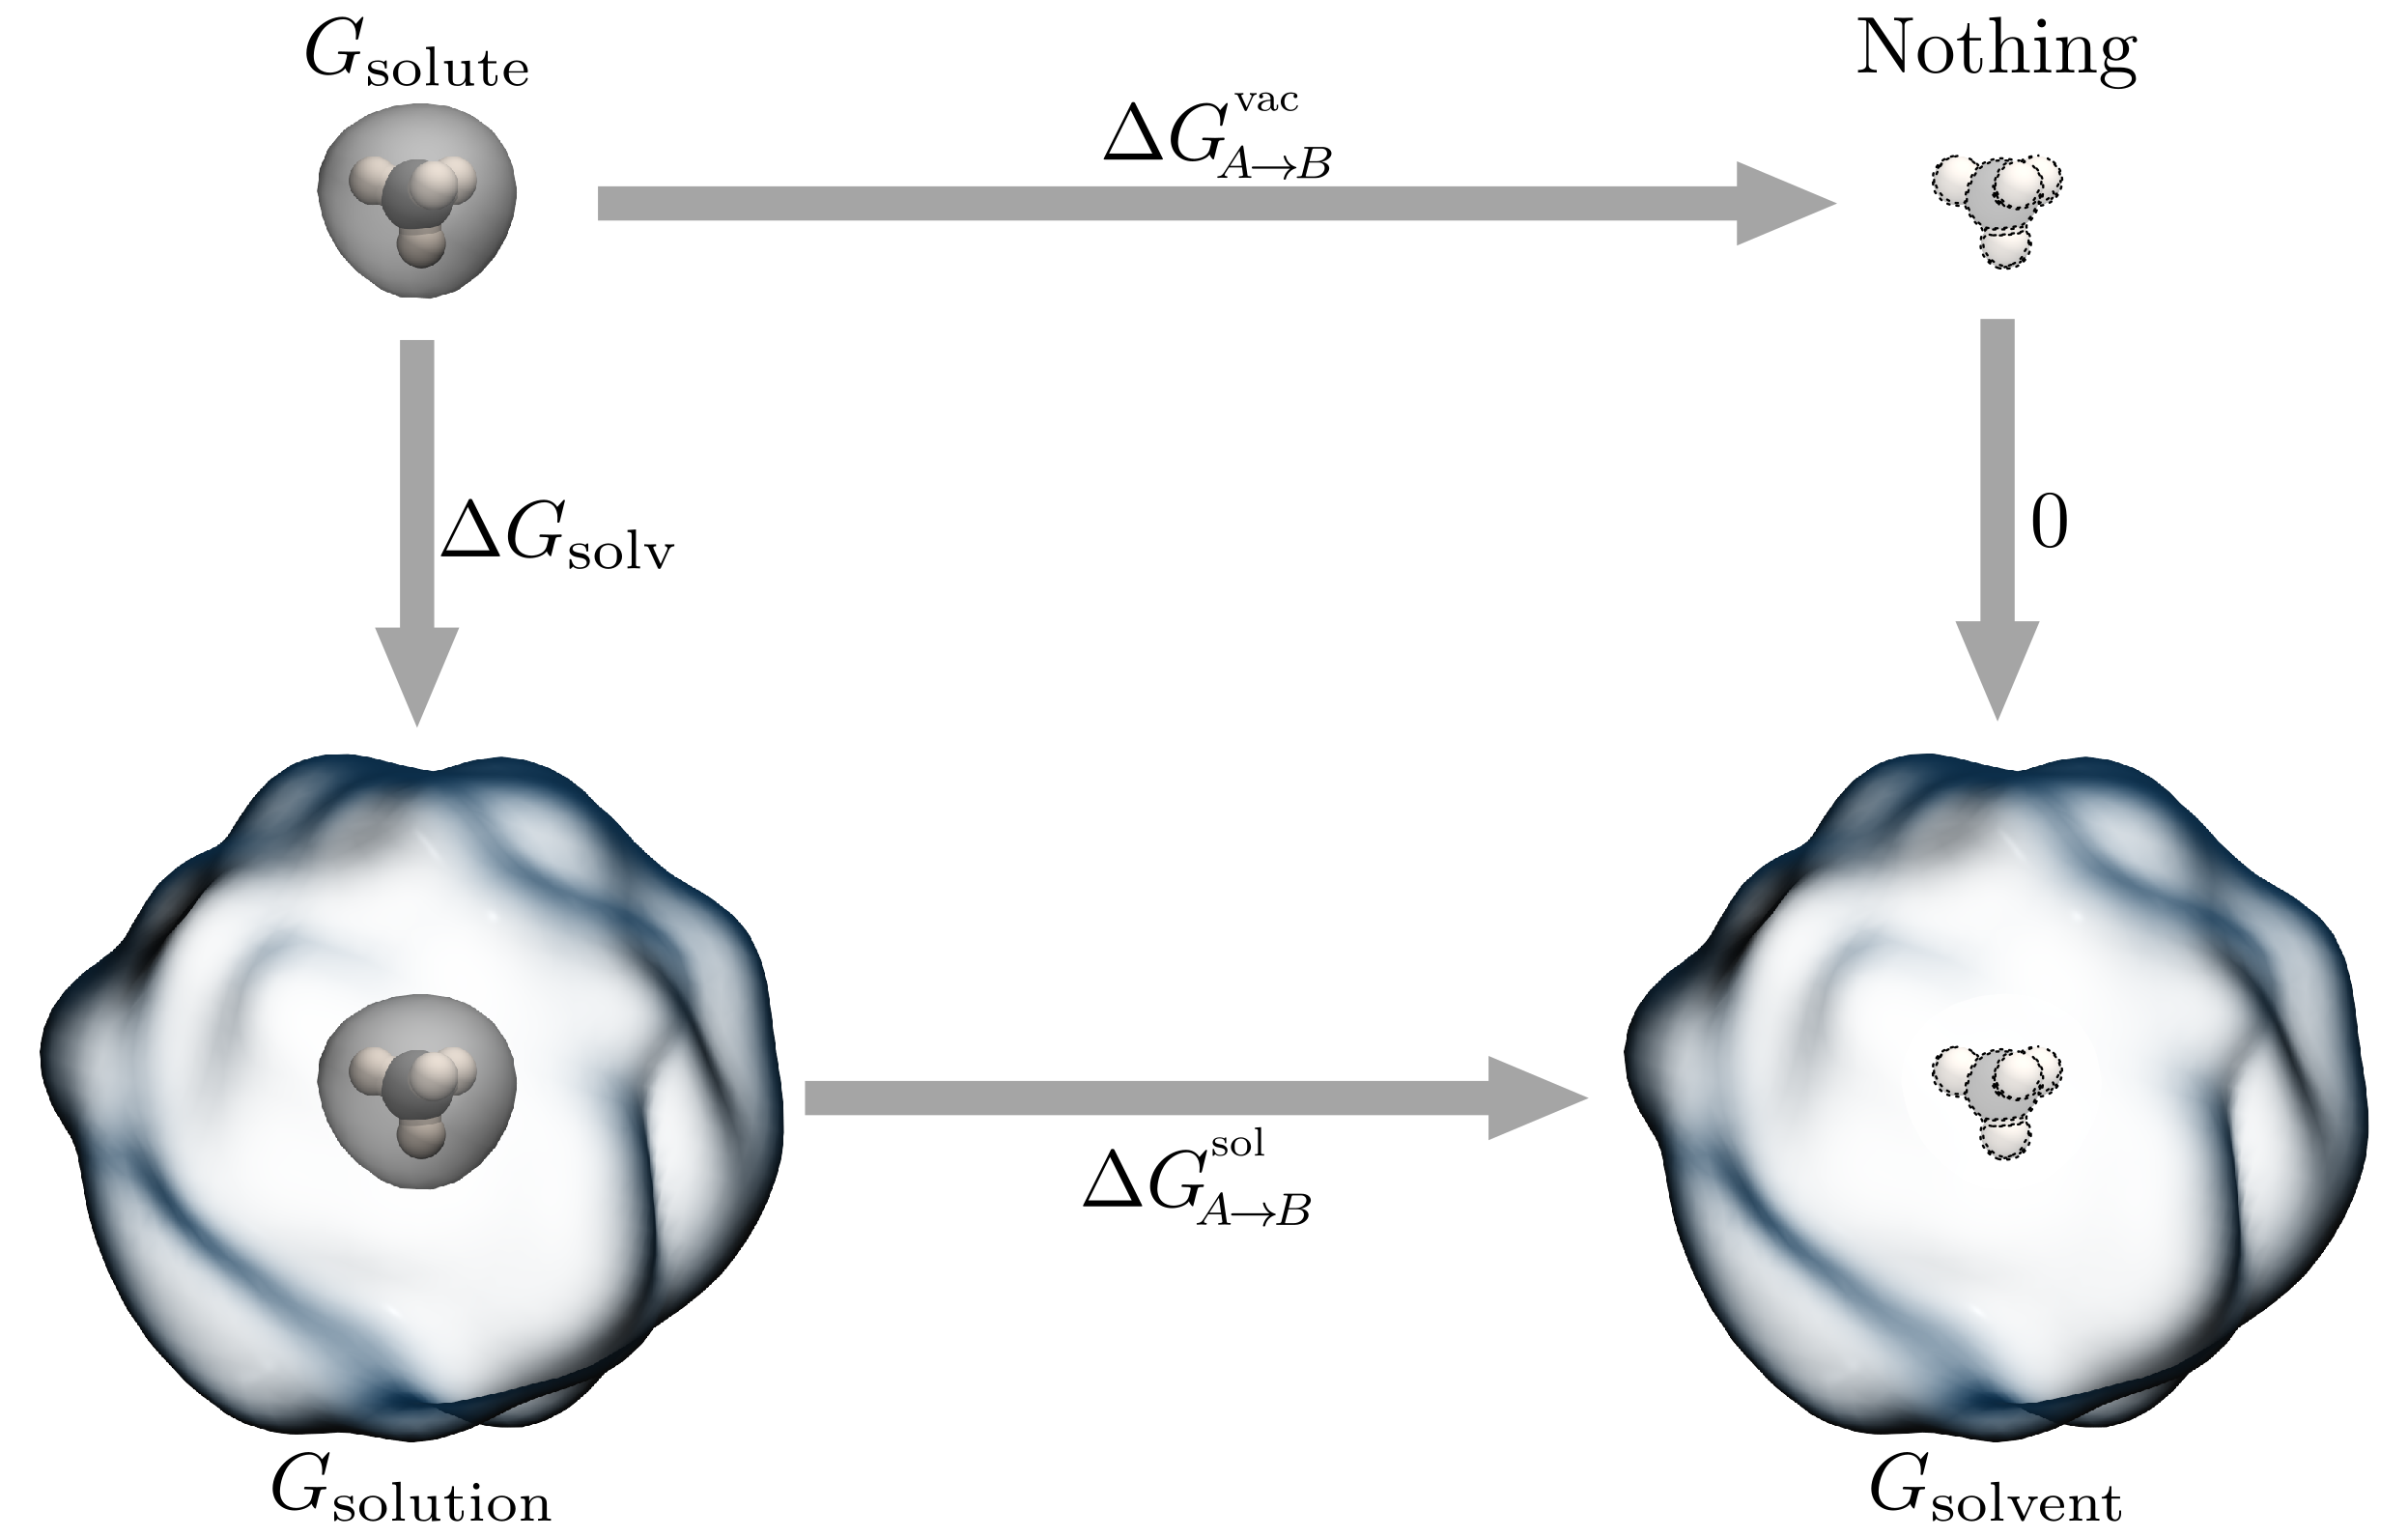
\includegraphics[width=0.48\textwidth]{figures/thermodynamicCycle.png}
    \caption{The solute, here a methane molecule, is transferred from a vacuum into water (left arrow). There are two intermediate systems shown on the right side. The upper only comprises the decoupled solute, visualized by transparency and dotted outlines, and the lower system shows the decoupled solute in the solvent. Each system is labeled with its respective term from \fref{eq:deltaGsolv}. In a thermodynamic cycle, only the end states matter; therefore, the alchemical route over two intermediate systems (three right arrows) can be chosen to indirectly obtain $\Delta G_\text{solv}$. The contribution from each arrow needs to be summed up, yielding the solvation free energy.}
    \label{fig:thermodynamiccycle}
\end{figure}

Therefore, the only contribution that is necessary to calculate the solvation free energy is $\Delta G_\text{\tiny A$\to$B}^{^\text{sol}}$, which denotes the alchemical annihilation of the solute within the aqueous solution. However, the annihilation cannot be conducted within a single simulation. A considerable energetic and conformational overlap must exist for two states to be eligible for free energy calculation.\\
% Hamiltonian concerning lambda
Therefore, the solute does not vanish in one step but via a multistep approach called the coupling strategy which is usually optimized by experienced scientist to enhance results. The coupling parameter $\lambda$ is introduced, which ranges between zero and one and specifies the decoupling progress from state $A$ ($\lambda=0$) to $B$ ($\lambda=1$). Theoretically, it can be applied to the complete Hamiltonian of the system containing the kinetic and potential energy or only to individual parts, e.g., the Lennard-Jones potential $U_{\varepsilon,\sigma}$ (part of the potential energy $U$).
\begin{align}
    U_{\varepsilon,\sigma}(r_\text{mn}, \lambda) & = \frac{(1-\lambda) C_{12}^\text{A} + \lambda C_{12}^\text{B}}{r_\text{mn}^{12}} - \frac{(1-\lambda) C_{6}^\text{A} + \lambda C_{6}^\text{B}}{r_\text{mn}^{6}} \\\label{eq:ljwithlambda}
    U_{\varepsilon,\sigma}(r_\text{mn}, \lambda) & = \frac{(1-\lambda) C_{12}^\text{A}}{r_\text{mn}^{12}} - \frac{(1-\lambda) C_{6}^\text{A}}{r_\text{mn}^{6}} \hspace{2cm} \Big| \,\, C_{12}^\text{B} = C_{6}^\text{B} = 0
\end{align}
The constants $C_{6}$ and $C_{12}$ are composite parameters containing $\varepsilon$ and $\sigma$. The formula is identical to \fref{eq:lennardJones}. The coupling strategy can be tuned to arbitrarily interpolate between both end states by selecting the appropriate $\lambda$ spacing. For every $\lambda$, a molecular dynamics (MD) simulation has to be performed to sample the system in each $\lambda$-state. This procedure can be understood as yet another thermodynamic cycle, applied to the only step that remained from \fref{fig:thermodynamiccycle}.
\begin{figure}[H]
    \centering
    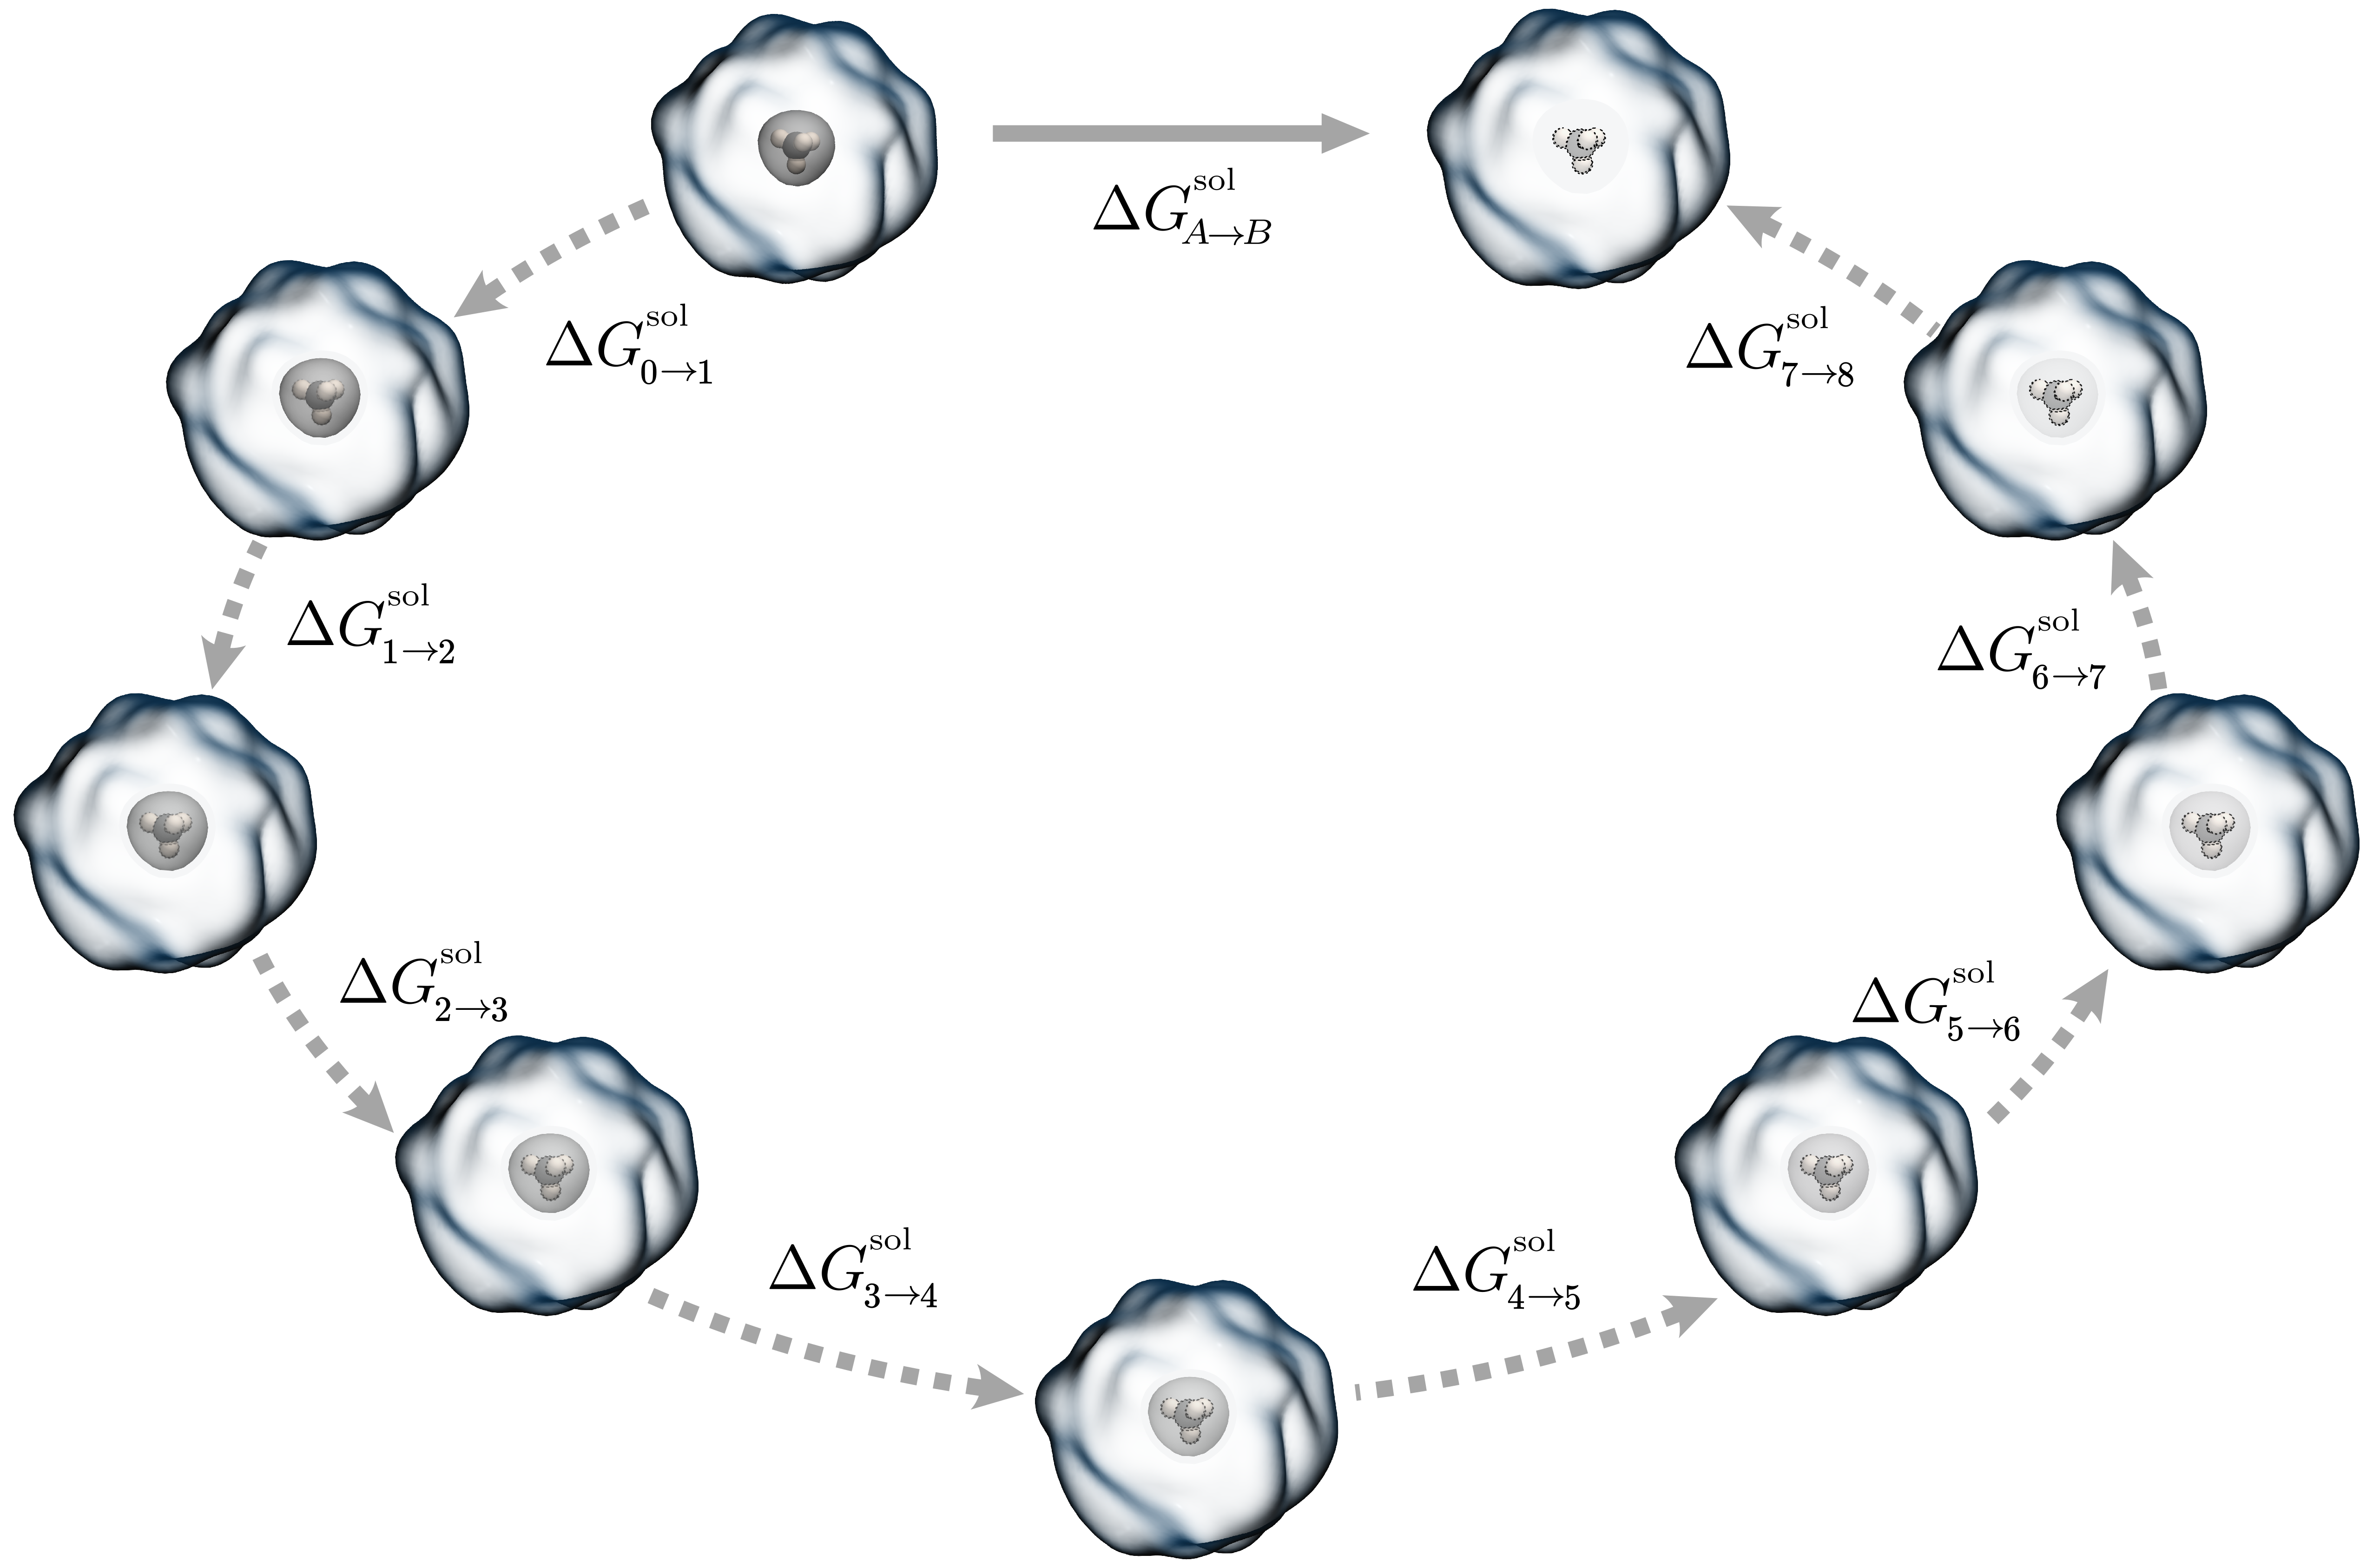
\includegraphics[width=0.48\textwidth]{figures/thermodynamicCycleLambda.png}
    \caption{Visualisation of the coupling/decoupling strategy. The direct but error-prone calculation of $\Delta G_\text{\tiny A$\to$B}^{^\text{sol}}$ is circumvented by a thermodynamic cycle that introduces seven unphysical intermediates utilizing the coupling parameter $\lambda_n$ that assumes values between zero and one. Each $\lambda$-state is simulated, and the free energy contributions are then calculated with an analysis method, e.g., the Bennett acceptance ratio (BAR) method.}
    \label{fig:thermodynamiccyclelambda}
\end{figure}

% The BAR method explained
The Bennett acceptance ratio (BAR) method\cite{Bennett1976} is the method of choice for calculating the contributions showcased in \fref{fig:thermodynamiccyclelambda}, i.e. $\Delta G_\text{\tiny i$\to$j}^{^\text{sol}}$ for the transition between to $\lambda$-states. The general idea is to sample configurations $X_\text{\tiny i}$ with the Hamiltonian that corresponds to a certain $\lambda_\text{i}$, $H(\lambda_\text{i})$. The Hamiltonian concerning a certain $\lambda$ can be rewritten as $U_\text{i}$ the potential energy since it is the only contribution affected by the decoupling strategy and for a consistent notation. The lengthy mathematical derivation can be looked up elsewhere\cite{Bennett1976}. Nonetheless, the final equation utilizes $X_\text{\tiny i} = \{x_1,...,x_\text{\tiny i},..., x_\text{\tiny M}\}$ and $X_\text{\tiny j} = \{x_1,...,x_\text{\tiny j},..., x_\text{\tiny N}\}$ the configurations sampled from two adjacent Hamiltonians (i.e. simulations) with sample sizes $N$ and $M$, and evaluates these configurations with their corresponding and each other's potential energy functions $U_\text{\tiny i}$ and $U_\text{\tiny j}$.
\begin{align}\label{eq:barmethod}
    \Delta G_\text{i$\to$j} & = \ln\left[\frac{\sum_{x_\text{\tiny j}}f(U_\text{\tiny i}(x_\text{\tiny j}) - U_\text{\tiny j}(x_\text{\tiny j}) + C)}{\sum_{x_\text{\tiny i}}f(U_\text{\tiny j}(x_\text{\tiny i}) - U_\text{\tiny i}(x_\text{\tiny i}) - C)}\right] + C - \ln(N/M) \\
    C & = \Delta G_\text{i$\to$j} + \ln(N/M)
\end{align}
Here, the function $f(x)$ is the Fermi function $f(x) = \frac{1}{1+\exp(x)}$, and the constant $C$ is to be determined by iteratively applying the above equations until the self-consistent results do not change anymore. 


\subsection*{Setup and Simulations}
Each part of this theoretical consideration has its computational counterpart. Due to the aforementioned relevancy of free energy calculations, this functionality has its own implementation via the \texttt{MDP} file. Also, the BAR analysis can be conducted using the \code{gmx bar} command. As usual, the forcefield and the system coordinates are given in the \texttt{TOP} and \texttt{GRO} files. It contains the methane molecule (called \texttt{ALAB}) and 750 TIP3P water molecules within the OPLS-AA forcefield approach. In the downloadable \texttt{TOP} file, the charges of the methane molecule are set to zero, which is appropriate since the Coulombic term is negligibly small according to Shirts et al.\cite{Shirts_2003}. Thus, incorporating a second decoupling strategy is here omitted.\\
The simulation phases comprise the usual energy minimization, NVT and NPT equilibrations, and production simulations. Every $\lambda$ value requires its own set of simulations. Herein, the decoupling strategy consists of 21 equidistant $\lambda$ values from 0 to 1, thus in steps of \num{0.05}. 
Two additional bash scripts can be downloaded, which ease housekeeping of the variety of different output files, \texttt{generate\_mdp\_files.sh} and (\code{run\_lambda\_simulations.sh}). The first one generates all necessary \texttt{MDP} files for running all simulation phases for each $\lambda$ from the downloadable source \texttt{MDP} files, and the second one executes all the runs in an automated fashion. However, these scripts are incomplete and must be augmented by the user where indicated. Once both scripts are fully functional, they can be executed in the following way:
\begin{lstlisting}[language=bash]
./generate_mdp_files.sh
\end{lstlisting}
This bash script will prompt the user to decide if a test run should be conducted first. A test run means that all \texttt{MDP} files will only run for 500 frames, drastically reducing the simulation time to a few minutes, even on older hardware. The dummy output files produce unreliable free energy estimates but still result in a functional BAR analysis (see below). Running the script in test mode is highly recommended and can be followed by denying the test run to generate \texttt{MDP} files with the appropriate number of frames as input for \code{run\_lambda\_simulations.sh}. Files generated with \code{generate\_mdp\_files.sh} are named, e.g., \texttt{em\_0.mdp}, \texttt{nvt\_1.mdp} or \texttt{prod\_19.mdp}. In addition to the usual options these files also specify the coupling/decoupling schemes. The corresponding free energy options provided by \texttt{GROMACS} are quite flexible and complex. The relevant ones are elaborated in \fref{tab:mdpoptions}. Although working parameters have been predetermined and adjusted in the source \texttt{MDP}, it is important to understand the free energy-related options before proceeding. For even further details, refer to the manual: \url{manual.gromacs.org/documentation/2023-beta/user-guide/mdp-options.html}
\onecolumn
\begin{center}
    \begin{tabularx}{\textwidth}{l X}
    \caption{Tabular description of parameters related to free energy calculations in \texttt{GROMACS}. On the left is the \texttt{MDP}-parameter with its corresponding value, and on the right is a brief description.}\\
    \toprule
    \texttt{free-energy = yes}          & Interpolate between topology A to topology B via the $\lambda$-states. Any $\lambda$-states would be ignored if this option would be set to no.\\
    \midrule
    \texttt{init-lambda-state = 0}     &  Specifies which column of the lambda vector should be used for the current simulation run. As shown below, $\lambda$-values are compiled into lists, and the corresponding column specifies the transition degree between states A and B. Zero means starting from the first column.\\
    \midrule
    \texttt{delta-lambda = 0}           & Increment per time step for $\lambda$. Instead of instantiating each $\lambda$-value and thus the alchemical transformation, the whole process can happen incrementally by specifying choosing non-zero for this option. However, this can result in serious errors and is therefore omitted.\\
    \midrule
    \texttt{calc-lambda-neighbors = 1} & Controls the number of lambda values for which Delta H values will be calculated. E.g., for a value of 1 and a \texttt{init-lambda-state} of 10, energy differences concerning $\lambda$-states 9 and 11 are computed.\\
    \midrule
    \texttt{vdw-lambdas = ...}         & A list of $\lambda$-values for the transformation of van der Waals interactions.\\
    \midrule
    \texttt{couple-moltype = Methane}  & Name given in the \texttt{TOP} file \texttt{[ moleculetype ]} section that is to be alchemically transformed from state A to state B.\\
    \midrule
    \texttt{couple-lambda0 = vdw}      & Tweaks the kind of non-bonded interactions that are present at $\lambda=0$. Here, charges are set to zero, and van der Waals interactions are considered.\\
    \midrule
    \texttt{couple-lambda1 = none}     & Tweaks the kind of non-bonded interactions that are present at $\lambda=1$. All non-bonded interactions will be turned off. Since the final $\lambda$ transition switches an infinity to zero, soft-core potentials are necessary to avoid singularities. Soft-core potentials modify the Lennard-Jones potential in a way that avoids infinite values.\\
    \midrule
    \texttt{couple-intramol = no}      & All intra-molecular non-bonded interactions for \texttt{[ moleculetype ]}  \texttt{couple-moltype} are replaced by exclusions and explicit pair interactions (as they would without \texttt{free-energy} set to \texttt{yes}).\\
    \midrule
    \texttt{nstdhdl = 10}              & The frequency for writing dH/d$\lambda$ and possibly Delta H to dhdl.xvg.\\
    \bottomrule
    \label{tab:mdpoptions}
    \end{tabularx}
\end{center}
\twocolumn
The $\lambda$ spacing might be the most important part of the alchemical route and is implemented within the $\lambda$ vectors in each \texttt{MDP} file. The $\lambda$ vectors for any \code{*.mdp} contains 20 columns and six rows.
\begin{lstlisting}
; init_lambda_state   0    1    2    3    4    5    6    7    8    9    10   11   12   13   14   15   16   17   18   19   20
vdw-lambdas         = 0.00 0.05 0.10 0.15 0.20 0.25 0.30 0.35 0.40 0.45 0.50 0.55 0.60 0.65 0.70 0.75 0.80 0.85 0.90 0.95 1.00
coul-lambdas        = 0.00 0.00 0.00 0.00 0.00 0.00 0.00 0.00 0.00 0.00 0.00 0.00 0.00 0.00 0.00 0.00 0.00 0.00 0.00 0.00 0.00
bonded-lambdas      = 0.00 0.00 0.00 0.00 0.00 0.00 0.00 0.00 0.00 0.00 0.00 0.00 0.00 0.00 0.00 0.00 0.00 0.00 0.00 0.00 0.00
restraint-lambdas   = 0.00 0.00 0.00 0.00 0.00 0.00 0.00 0.00 0.00 0.00 0.00 0.00 0.00 0.00 0.00 0.00 0.00 0.00 0.00 0.00 0.00
mass-lambdas        = 0.00 0.00 0.00 0.00 0.00 0.00 0.00 0.00 0.00 0.00 0.00 0.00 0.00 0.00 0.00 0.00 0.00 0.00 0.00 0.00 0.00
temperature-lambdas = 0.00 0.00 0.00 0.00 0.00 0.00 0.00 0.00 0.00 0.00 0.00 0.00 0.00 0.00 0.00 0.00 0.00 0.00 0.00 0.00 0.00
\end{lstlisting}
Although \code{vdw-lambdas} is the only non-zero row, the others are still listed to showcase what else might be specified. The option \texttt{init-lambda-state = 0} specifies the Hamiltonian with the 0-th element in the \texttt{vdw-lambdas} list, here \code{0.00}. Setting \texttt{initial-lambda-state = 1} would correspond to the next element, i.e. \code{0.05}, while \texttt{initial-lambda-state = 20} would specify the final column, resulting in a $\lambda$-value of \code{1.00} for van der Waals interactions meaning they would be turned off completely according to \fref{eq:ljwithlambda}.\\
The other bash script is called \code{run\_lambda\_simulations.sh}. It also needs to be completed, and one of the tasks is to fill in the gaps and append code suggestions to the report. After successful completion, \code{run\_lambda\_simulations.sh} should first create the following directory hierarchy:
\begin{lstlisting}
lambda_0/
lambda_1/
lambda_2/
lambda_3/
lambda_4/
\end{lstlisting}
This way, all steps in the workflow are executed within a single directory for each value of \texttt{init-lambda-state}, which is a convenient way to organize the simulations and their output. Then, the aqueous methane system is simulated, and if no error occurs, the terminal output should look something like the below:
\begin{lstlisting}
Starting minimisation for lambda = 0 ...

    ##############################
    # ENERGY MINIMIZATION STEEP  #
    ##############################


    ##############################
    #     NVT EQUILIBRATION      #
    ##############################


    ##############################
    #     NPT EQUILIBRATION      #
    ##############################


    ##############################
    #        PRODUCTION MD       #
    ##############################
    .
    .
    .
\end{lstlisting}
However, should there be a mistake, the bash script should report an error to the user, as seen below.
\begin{lstlisting}
Starting minimisation for lambda = 0 ...

    ##############################
    # ENERGY MINIMIZATION STEEP  #
    ##############################

something went wrong, check /long/absolute/path/to/lambda_0/em/mdrun.em
\end{lstlisting}
Notice how the bash script specifies a file containing more information on what might have caused the error. All the simulations should be executed automatically since the missing parts were filled in correctly. The whole workflow can take quite a long time (\textbf{about 8 hours on 4 CPUs}); therefore, the simulations should be started as early as possible. Once the production simulations are complete, the resulting data can be analyzed.\\
Utilizing bash scripts can be a double-edged sword. Firstly, writing a correctly working bash script takes time; sometimes, it could take longer than setting things up manually. Secondly, if there is an error somewhere in the bash script, simulations will not finish or end up the way they were intended, and the whole bash script must be executed again.\\
However, both these drawbacks can be mitigated. Firstly, looking at the workload of this exercise, there is a total of 84 simulations to run. Seamlessly executing all \code{gmx grompp} and \code{gmx mdrun} commands by hand would take a long time, so a bash script is worth it. Secondly, bash scripts have numerous benefits, like reproduction, documentation, and they can be reused, to name just a few. Last but not least, the fun and challenge of coming up with a working bash script is not to be underestimated as a motivating factor.\\


\subsection*{Analysis}
The BAR module of \texttt{GROMACS} calculates $\Delta G_{solv}$. Therefore, all \code{prod.xvg} files produced by \code{run\_lambda\_simulations.sh} must be included in the \code{gmx bar} command, which can be achieved by copying all the files in a shared directory or (easier) by specifying the correct \texttt{GLOB}. The correct command can be seen below if the directory structure is unchanged.
\begin{lstlisting}
gmx bar -f lambda_*/prod.xvg -o -oi
\end{lstlisting}
In addition to producing \code{bar.xvg}, \code{barint.xvg}, and \code{histogram.xvg}, the program will print lots of useful information to the terminal, which should look something like this:
\begin{lstlisting}
Detailed results in kT (see help for explanation):

 lam_A  lam_B      DG   +/-     s_A   +/-     s_B   +/-   stdev   +/- 
     0      1    0.08  0.00    0.03  0.00    0.04  0.00    0.24  0.00
     .      .    ....  ....    ....  ....    ....  ....    ....  ....
     .      .    ....  ....    ....  ....    ....  ....    ....  ....
    19     20   -0.05  0.00    0.00  0.00    0.00  0.00    0.10  0.00

Final results in kJ/mol:

point      0 -      1,   DG  0.19 +/-  0.00
.....      . .      ..   ..  .... ...  ....
.....      . .      ..   ..  .... ...  ....
.....      . .      ..   ..  .... ...  ....
point     19 -     20,   DG -0.13 +/-  0.00

total      0 -     20,   DG -9.23 +/-  0.07
\end{lstlisting}
Examining the content of the output files is essential, as they provide a comprehensive understanding of the decoupling process and the effectiveness of the sampling. From the \texttt{DG} values (corresponding to $\Delta G_\text{\tiny i$\to$j}^\text{\tiny sol}$ in \fref{fig:thermodynamiccyclelambda}), it becomes evident that some transitions lead to an increase in the free energy of solvation, while others improve the solvation of methane. The values printed for \texttt{s\_A} and \texttt{s\_B} represent the configurational overlap between states $A$ and $B$. This information is crucial for assessing the adequacy of sampling and the reliability of the calculated free energy measures.\cite{Wu_2005}\\
The \code{bar.xvg} file contains the relative free energy differences for each $\lambda$ interval (i.e., between neighboring Hamiltonians). It should look similar to \fref{fig:barxvg} when plotted with \texttt{xmgrace}.
\begin{figure}[H]
    \centering
    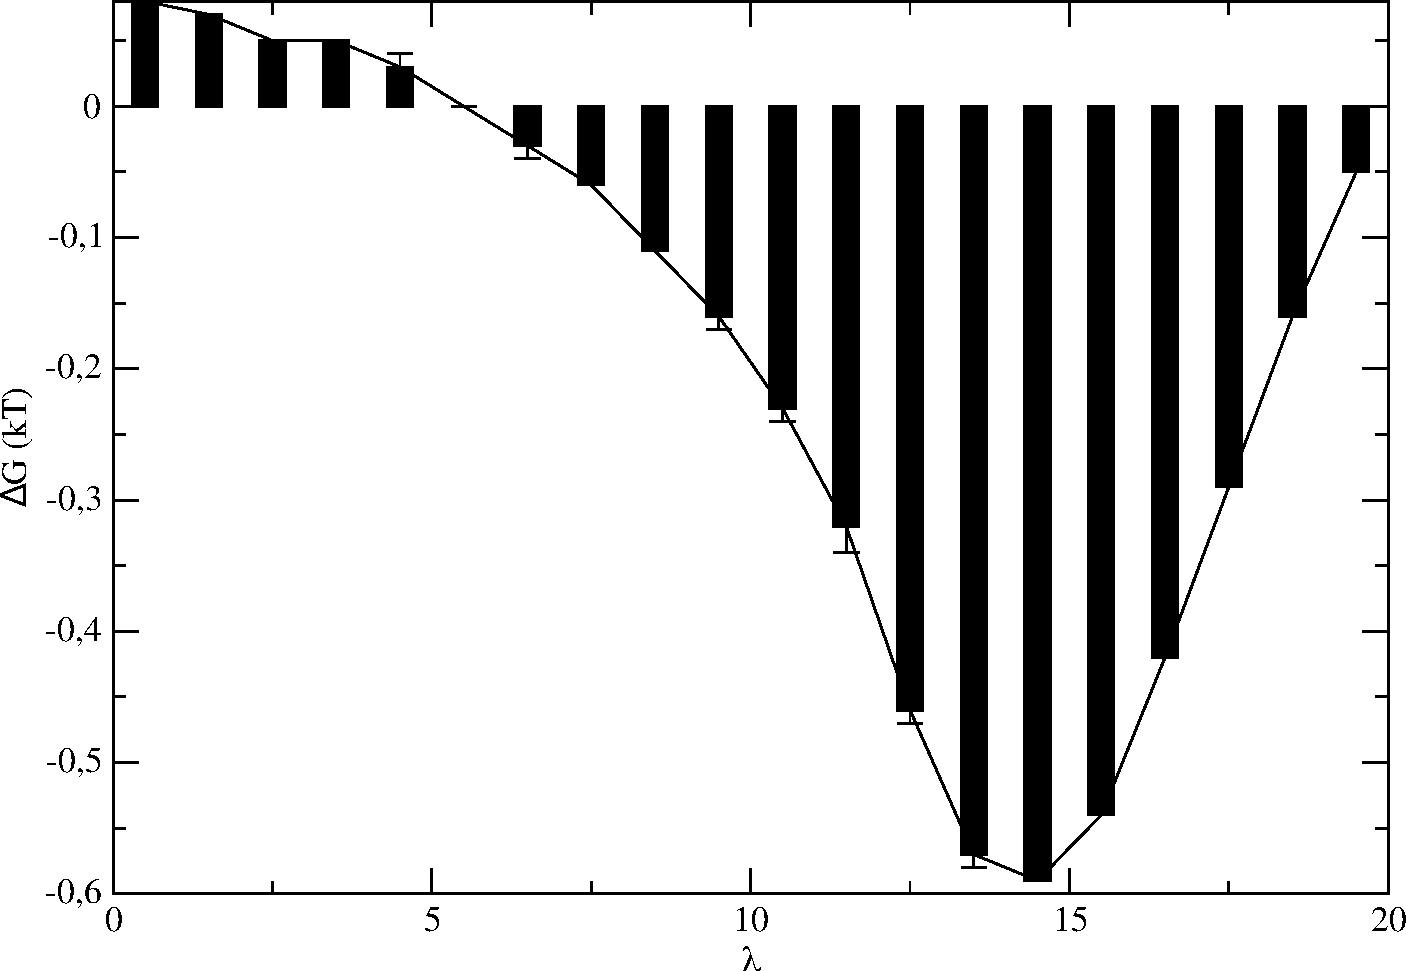
\includegraphics[width=0.48\textwidth]{figures/bar_xvg.pdf}
    \caption[Bar Plot of the Relative Free Energy Differences.]{The x-axis contains the discrete $\lambda_i$ values utilized in the decoupling process conducted here. The y-axis contains the relative free energy difference between two neighboring $\lambda_\text{\tiny i}$ values shown as black bars.}
    \label{fig:barxvg}
\end{figure}
The free energy differences between simulation $i$ and simulation $i+1$ are calculated via \fref{eq:barmethod}. \texttt{GROMACS} does not use the configurations but instead directly writes out the potential energies $U_\text{\tiny i}(x_\text{\tiny j})$, $U_\text{\tiny i}(x_\text{\tiny i})$ and so on, every \texttt{nstdhdl = 10} steps. The total solvation free energy can be obtained by summing up all these intermediate free energy changes.\\
The \code{barint.xvg} file plots the cumulative $\Delta G$ as a function of $\lambda$. Thus, $\lambda_{20}$ corresponds to the sum of $\Delta G$ from $\lambda_0$ to $\lambda_{20}$. In \fref{fig:barintxvg} \code{barint.xvg} is shown together with the data of \code{bar.xvg} illustrating the cumulative $\Delta G$.
\begin{figure}[H]
    \centering
    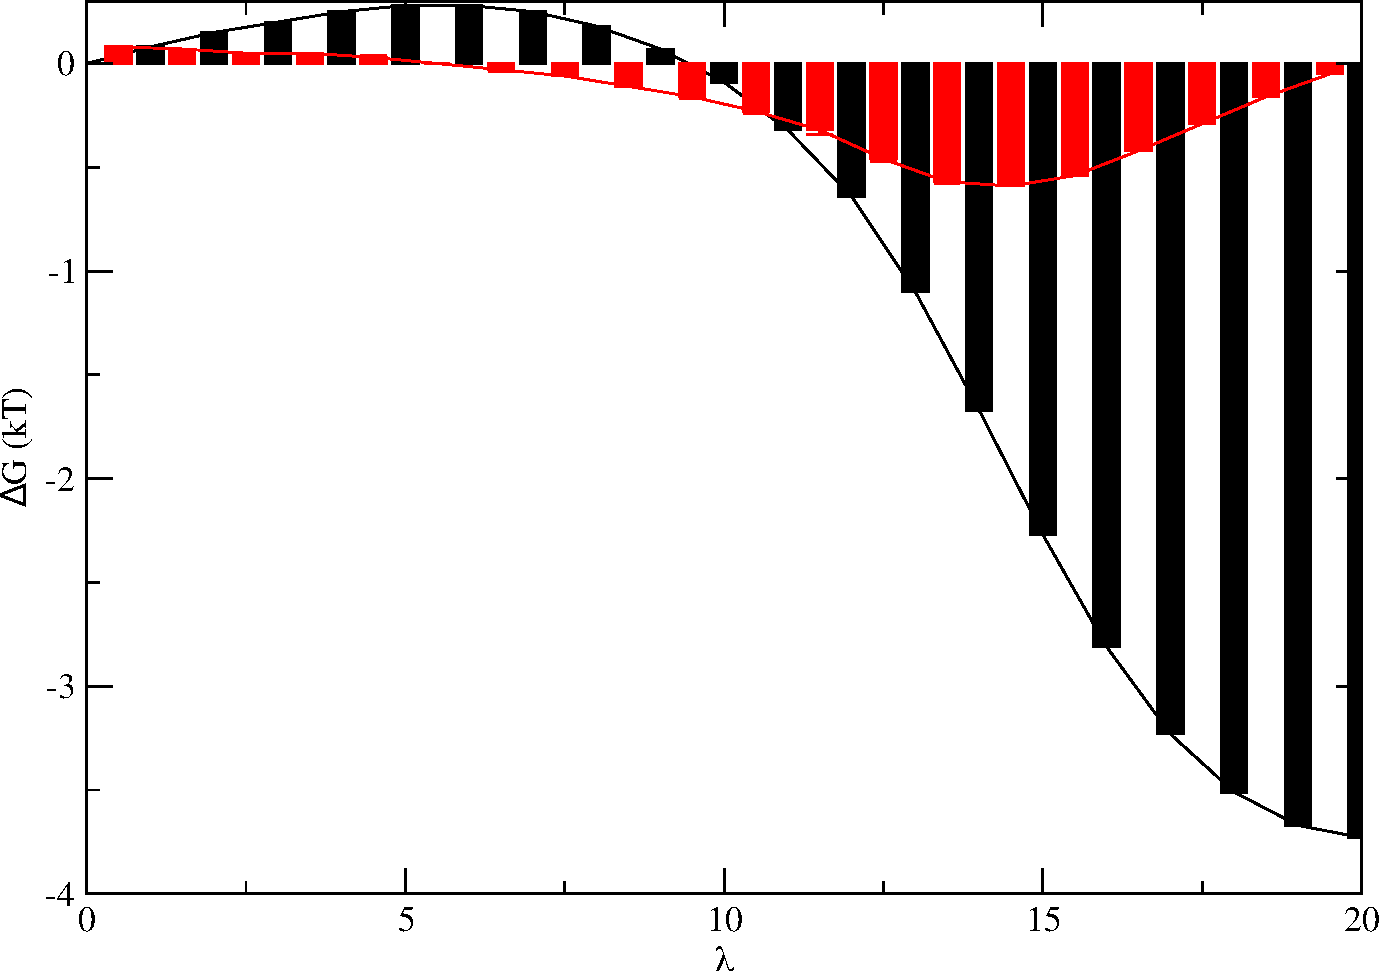
\includegraphics[width=0.48\textwidth]{figures/bar_and_barint_xvg.pdf}
    \caption[Cumulative Bar Plot of the Free Energy.]{The x-axis contains the $\lambda$-increments, and the y-axis shows the free energy difference in units of $kT$. Additionally to the black bars, the cumulative free energy differences are shown as red bars.}
    \label{fig:barintxvg}
\end{figure}
By taking the value of $\Delta G$ at $\lambda_{20}$, we can recover the value of $\Delta G_\text{\tiny solv}$ by converting from $kT$ to \SI{}{\kilo\calorie\per\mole}. The literature value for the solvation free energy of methane is \SI[separate-uncertainty]{2.42(1)}{\kilo\calorie\per\mole} (see Shirts et al.\cite{Shirts_2003}. Report the output from \code{gmx bar} and how well your simulation setup reproduces the literature value. Increasing the simulation time or decreasing the lambda spacing may lead to improved agreement with the publication, but this would be voluntary. Apart from these two possibilities, the report should discuss other options that may increase the accuracy of the results.

\newpage

\section{Exercise 7: Potential of Mean Force of an Amyloid Layer Separation via Umbrella Sampling}\label{sec:freeEnerBind}
\begin{Checklists}
    \begin{checklist}{Tasks for the Seventh Exercise}
    \textbf{Finish these tasks and write a short report about your findings.}
    \begin{itemize}
		\item Comment \code{02\_simprep.sh} line by line and include it in the report (as a screenshot or similar).
		\item Include plots of the histograms and the PMF and discuss their appearance.
		\item Report your result for $\Delta G_\text{bind}$ and compare it to the literature (\SI{-50.5}{\kilo\calorie\per\mole}).
	\end{itemize} 
    \end{checklist}
\end{Checklists}


\subsection*{Acknowledgement}
This exercise was inspired by a tutorial offered by Justin Lemkul\cite{Lemkul2019}.


\subsection*{Introduction}
This exercise explores the usefulness and applicability of free energy calculations, building on the previous exercise, which focused on solvation free energy via alchemical transformations. Here, we estimate the free energy of binding by sampling two binding partners at various spatial distances. The larger binding partner is usually called the receptor, and the smaller one is the ligand. Receptor-ligand complexes are crucial in biomolecular signal transduction, enzymatic catalysis, and therapeutic efficacy.\cite{Gumbart_2012} Binding free energy - the energy change when a ligand binds to its receptor - is fundamental in understanding these processes. As with solvation free energy, there are many approaches to obtaining the binding free energy, each with its strengths and weaknesses.\\
For this exercise, we analyze the A\textbeta(1-42) amyloid fibril associated with Alzheimer's disease using molecular dynamics (MD) simulations.\cite{L_hrs_2005} This amyloid protofilament consists of five peptides with beta sheets interconnected via their side chains. The 42 amino acid-long peptides are part of the protofilaments.\cite{Benson_2020} In a series of simulations, the terminal peptide of the protofilament is pulled away from the remaining amyloid fibril. It is extensively sampled along the distance coordinate, also known as a \textit{collective variable}. Sampling along this collective variable is achieved using harmonic biasing potentials in a procedure known as umbrella sampling (US) simulations.\cite{Torrie_1977} This method results in distance distributions that resemble an umbrella shape. The sampling data is then evaluated using an advanced algorithm to produce a free energy surface, from which the pulling free energy is obtained.\cite{Kumar_1992}\\
Lemkul and Revan precisely calculated the potential of mean force ($\Delta G_\text{\tiny bind}$) for this system, predicting a value of \SI{-50.5}{\kcalm}.\cite{Lemkul_2010} this exercise aims to replicate this value using \texttt{GROMACS} built-in functionalities for conducting umbrella sampling simulations.


\subsection*{Theoretical Considerations}
\begin{figure}[H]
    \centering
    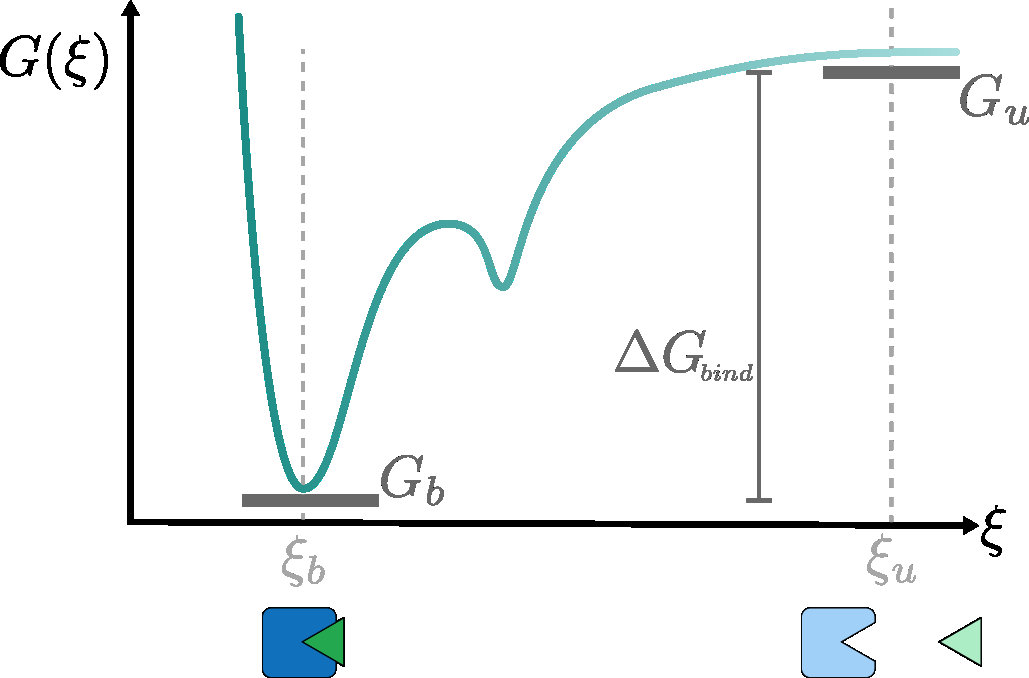
\includegraphics[width=0.48\textwidth]{figures/GofXiAnnotated.png}
    \caption{Visualisation of the binding process along the collective variable $\xi$. The free energy $G$ approaches a minimum for the bound state, described by $\xi_b$. For further clarification, the bound and unbound complexes are depicted with geometrical shapes beneath the x-axis.}
    \label{fig:GofXiAnnotated}
\end{figure}
The binding free energy $\Delta G_\text{\tiny bind}$ is generally defined as the difference between the free energy of the bound state $G_\text{b}$ and the unbound state $G_\text{u}$. Thus, the binding free energy represents the reversible work released during complex association. The free energies of the bound and unbound states are related to the average probability $\langle P \rangle$ of encountering these states in a given environment, such as an aqueous solution.\cite{Woo_2005}
\begin{align}\label{eq:deltaGbind}
    \Delta G_\text{\tiny bind} = G_\text{b} - G_\text{u}  =  -k_\text{B} T \ln\left(\frac{\langle P_\text{b} \rangle}{\langle P_\text{u} \rangle} \right)
\end{align}
The probabilities given in \fref{eq:deltaGbind} can be defined concerning an arbitrary \textit{collective variable} $\xi$ along which the binding can be described. For ligand binding phenomena, a classical choice for $\xi$ is the center-of-mass (COM) distance with the receptor, denoted as $r_\text{\tiny com}$. However, any observable can be chosen for $\xi$, e.g., dihedral angles or RMSDs. The average probability of encountering a certain $r_\text{\tiny com}$ distance can be obtained only via the partition function, $Z_\text{\tiny NPT}$.
\begin{align}\label{eq:PofRcom}
    \langle P(r_\text{\tiny com}) \rangle = \frac{\int_\mathbf{X} d\mathbf{X} \, \delta(r_\text{\tiny com} - R_\text{\tiny com}(\mathbf{X})) e^{ -\beta H(\mathbf{X}) }} {Z_\text{\tiny NPT}}
\end{align}
The function $R_\text{\tiny com}(\mathbf{X})$ evaluates the COM of the configuration $\mathbf{X}$ and is compared to an arbitrary $r_\text{\tiny com}$ value via the Dirac delta function, $\delta(...)$. Integration occurs over all configurations of the system, $\int_\mathbf{X}$, causing the dependency on $\mathbf{X}$ to vanish for $\langle P(r_\text{\tiny com}) \rangle$. The bound and unbound states can now be defined concerning the reaction coordinate: beyond a certain COM distance threshold, the intermolecular interactions cease; thus, the binding partners are considered fully separated.\\
Unfortunately, this equation cannot obtain $\Delta G_\text{\tiny bind}$ from simulation since the system's partition function is practically unobtainable. The intermolecular attraction is so high for tightly bound complexes that dissociation events would never be sampled within feasible MD simulation times. Therefore, a different approach is used, employing harmonic potentials along the COM distance to enhance sampling across all regions of the binding/unbinding process. The exact \textit{stratification strategy} may vary, but typically, for binding processes, multiple simulations ($s$) are conducted, each with a biasing potential $U_s$ resembling a harmonic spring potential. This potential is defined by the spring constant $k_s$ and the equilibrium COM distance $r_\text{\tiny com}^s$.
\begin{align}\label{eq:umbrellaBiasingPotential}
    U_s(r_\text{\tiny com}) & = k_s \left( r_\text{\tiny com}^s - r_\text{\tiny com} \right)^2
\end{align}
Each biased simulation results in a biased probability distribution, $P^s_\text{\tiny com}$, that preferentially samples $r_\text{\tiny com}$ values close to the reference distance $r^s_\text{\tiny com}$ (see \fref{fig:umbrellaSamplingConcept}).
\begin{figure}
    \centering
    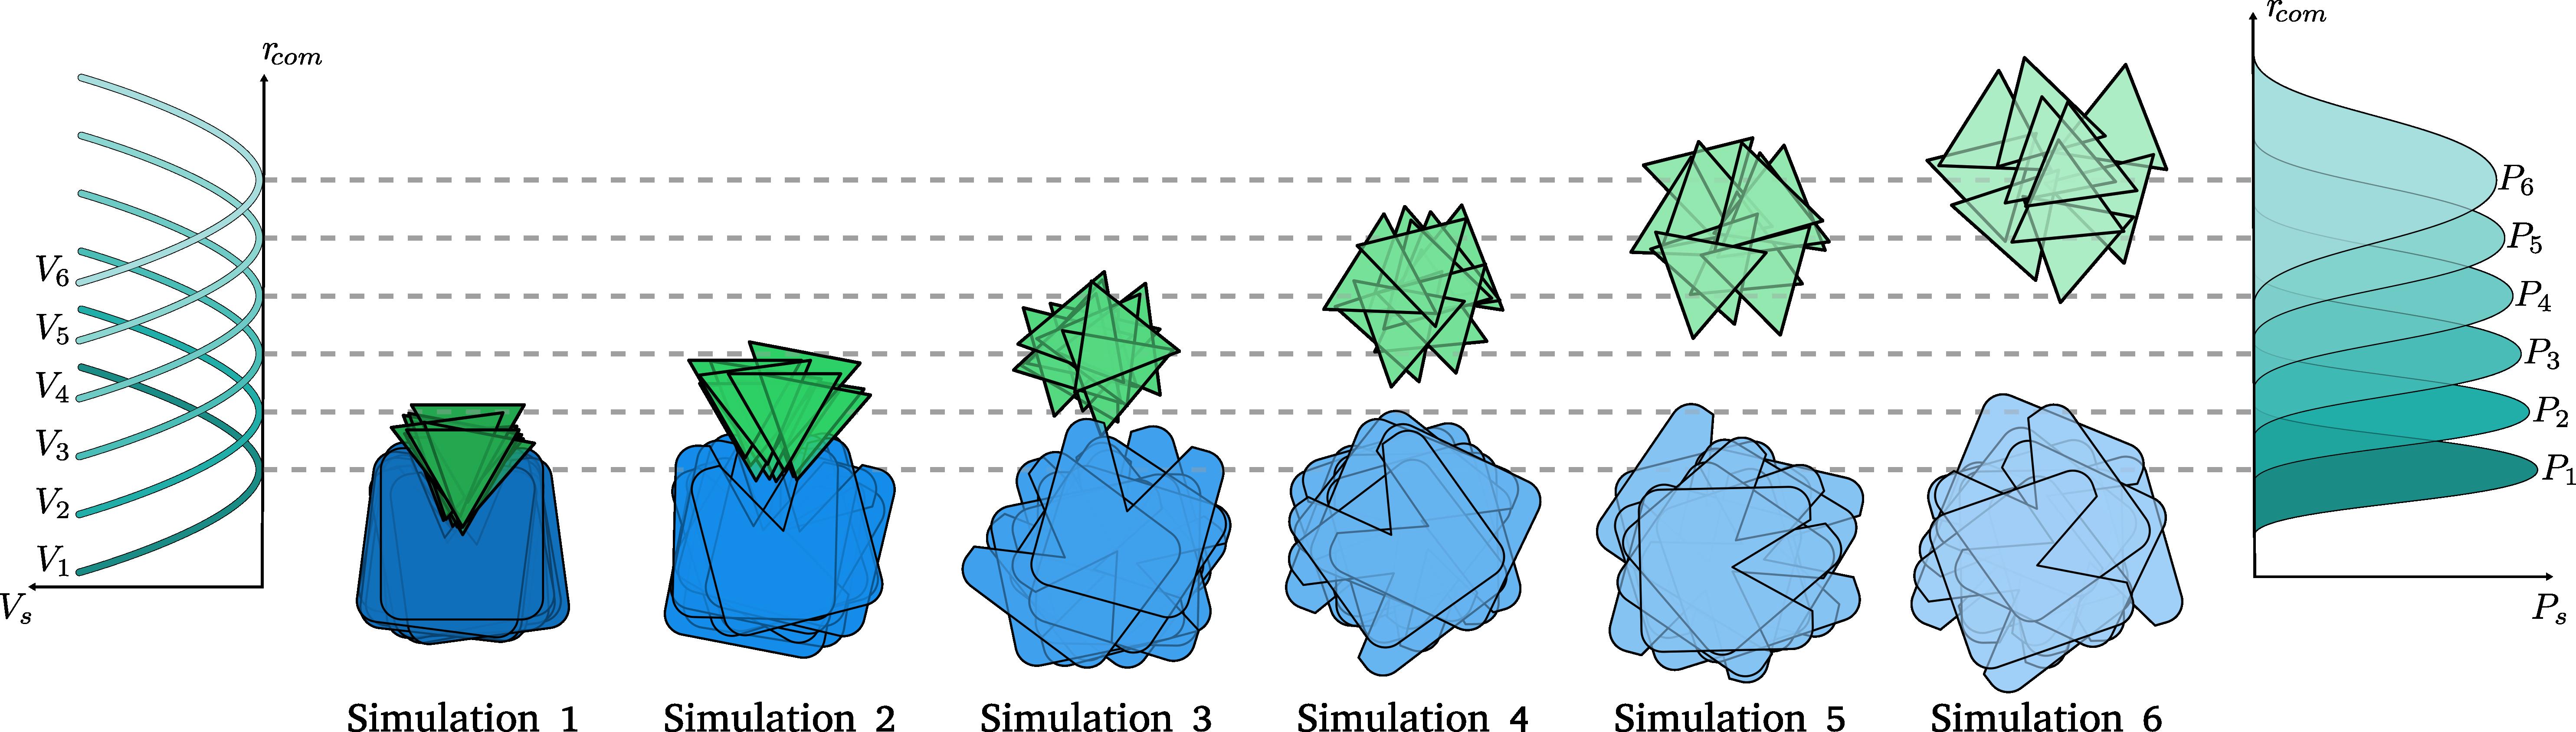
\includegraphics[width=0.48\textwidth]{figures/umbrellaSamplingConcept.png}
    \caption{Conceptual visualization of umbrella sampling for an arbitrary receptor-ligand complex. The harmonic potentials on the left keep the ligand (green triangle) restrained at a certain distance from the receptor (blue rectangle). The sampling is visualized via superimposed copies of the respective molecules in the six simulation windows. The resulting COM distances are shown in the graph on the right as probability distributions.}
    \label{fig:umbrellaSamplingConcept}
\end{figure}
However, it can be shown mathematically that the expression for $P^s_\text{\tiny com}$ still depends on the partition function $Z_\text{\tiny NPT}$ and the unbiased probability distribution $\langle P(r_\text{\tiny com}) \rangle$.\cite{Kumar_1992}
\begin{align}
    \langle P_s(r_\text{\tiny com}) \rangle =  \frac{Z_\text{\tiny NPT}}{Z^{^s}_\text{\tiny NPT}} \langle P (r_\text{\tiny com}) \rangle e^{-\beta U_s(r_\text{\tiny com})}
\end{align}
This equation can be rearranged for the unbiased probability as follows:
\begin{align}
    \langle P(r_\text{\tiny com}) \rangle = \langle P_s (r_\text{\tiny com})\rangle \cdot \frac{\langle e^{-\beta U_s(r_\text{\tiny com})} \rangle}{e^{-\beta U_s(r_\text{\tiny com})}}
\end{align}
Seemingly, not much is achieved by performing multiple simulations with biasing potentials, as $\langle P(r_\text{\tiny com}) \rangle$ and the unbiased partition function remain unknown. The partition function of the biased simulation would also need to be calculated. Nevertheless, Ferrenberg and Swendsen\cite{Ferrenberg_1988} developed the weighted histogram analysis method (WHAM),\cite{Roux_1995} which employs similar mathematical techniques to those implemented in the BAR method from \fref{sec:freeEnerSolv}.\cite{Bennett1976} WHAM operates using histograms of the collective variable; instead of continuous values of $r_\text{\tiny com}$, only certain histogram bins with their center values $i$ are considered.\\
The lengthy and complex derivation of the WHAM equations is beyond the scope of this document. However, the resulting two equations will be discussed in detail. The objective is to accurately estimate the unbiased, discretized probability distribution $\langle P(i) \rangle$. Sampled COM distances from each simulation are collected and binned into a histogram with $N_\text{\tiny bins}$, chosen by the user. Consequently, the resulting histogram $h_s(i)$ from simulation $s$ should contain counts mostly close to the reference distance given by the corresponding harmonic potential $U_s$. The sum of all simulation histograms is then divided by a self-consistent term, determined iteratively (see also \fref{fig:whamAlgorithm}).\cite{Hub_2010}
\begin{align}\label{eq:whamequations}
    \langle P(i) \rangle = \frac{\sum\limits_s^{N_\text{\tiny sims}} h_s(i)}{\sum\limits_s^{N_\text{\tiny sims}} n_s \cdot \exp\left(-\beta (U_s(i) - f_s)\right)}\\[0.3cm]
    f_s = -k_B T \ln \left( \sum_i^{N_\text{\tiny bins}} \langle P(i) \rangle \cdot \exp\left(-\beta U_s(i)\right) \right)
\end{align}
The so-called free energy constants $f_s$ are initialized to zero and approach convergence after a certain number of iterations.\cite{Kumar_1992} These constants correspond to the free energy of the biased simulation $s$ but do not relate directly to the free energy of binding. To obtain $\Delta G_\text{\tiny bind}$, the unbiased probability $\langle P(i) \rangle$ is used to calculate a free energy surface (FES) $G(i)$.\cite{Hub_2010}
\begin{align}
    G(i) & = -k_B T \ln \left(\frac{\langle P(i)\rangle }{ \langle P_\text{\tiny max} \rangle} \right) 
\end{align}
Dividing by the maximum of the probability distribution shifts the minimum $G(i)$ to zero. This zero-shift is common practice since the free energy surface can only be calculated up to a constant, and free energy differences are usually of interest (compare \fref{fig:GofXiAnnotated}).
\begin{figure}
    \centering
    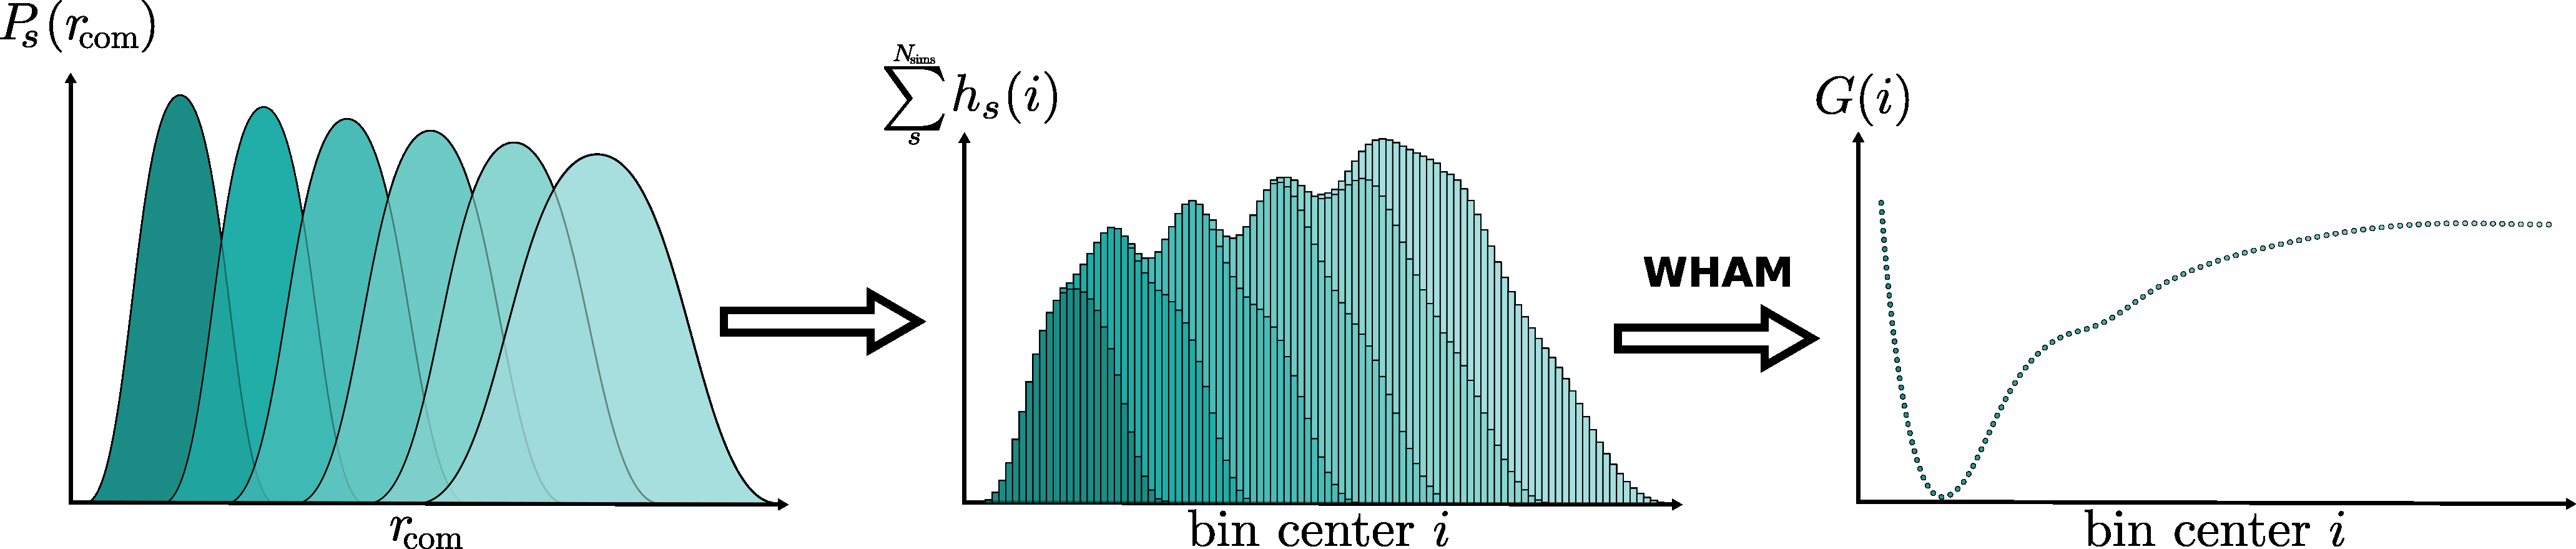
\includegraphics[width=0.48\textwidth]{figures/whamAlgorithm.png}
    \caption{Depiction of data generation and the WHAM algorithm. The COM distances are collected from the $N_\text{\tiny sims}$ simulations. The binned histograms are summed, and then the WHAM equations are applied iteratively until the unbiased probability distribution $\langle P(i) \rangle$ emerges, from which the free energy surface $G(i)$ can be readily obtained.}
    \label{fig:whamAlgorithm}
\end{figure}


\subsection*{Setup and Simulations}
The computational implementation of the described theoretical background is completely implemented in the \texttt{GROMACS} software. However, the specifics are still quite complicated. The steps can be categorized into obtaining equilibrated molecular coordinates and topologies, generation of initial configurations along the $r_\text{\tiny com}$ coordinate via a pulling simulation, and eventually, the umbrella sampling simulations, which can be subcategorized in equilibration and production simulations. The latter step can take several days. Therefore, it is recommended that these simulations start as soon as possible. Should the following analysis reveal missing bins in the histograms or generally deviating free energy results, additional sampling can be conducted in regions with insufficient sampling, so-called post-sampling. The analysis can then be rerun, incorporating the new data, hopefully leading to an improved result.\\
The system of interest is the A\textbeta(1-42) amyloid protofilament consisting of five peptides, and the process that shall be investigated is the dissociation of the terminal peptide. The protein complex has the PDB identifier 2BEG and can be downloaded from the PDB databank or the online repository (recommended). Apart from the original \texttt{PDB} file, the other necessary files entail the \texttt{TOP}, \texttt{GRO}, and \texttt{MDP} files. Both the \texttt{TOP} and \texttt{GRO} files can be created by \texttt{GROMACS}' toolkit, but the \texttt{MDP} files need to be downloaded from the online repository. Most US-specific differences are concentrated in the \texttt{MDP} file. However, this time, the \texttt{TOP} file will require slight alteration, and the \texttt{GRO} file will be elongated to better encompass the separation instead of its usual cube shape.\\
The \texttt{GROMACS} input files are generated in the usual way, firstly converting the \texttt{PDB} to a \texttt{GRO} file, specifying the box and then solvating it, followed by ion generation. The commands can be found below. The resulting file that can be forwarded for minimization is called \code{solv\_ions.gro}.
\begin{lstlisting}[language=bash]
gmx pdb2gmx -f 2BEG_model1_capped.pdb -ignh -ter -o complex.gro  # Choose GROMOS96 53A6; SPC; all N-termini: None; all C-Termini COO-
gmx editconf -f complex.gro -o newbox.gro -center 3.280 2.181 2.4775 -box 6.560 4.362 12  # box size complies with minimum image convention and extend of pulling
gmx solvate -cp newbox.gro -cs spc216.gro -o solv.gro -p topol.top  # solvate with SPC water
gmx grompp -f ions.mdp -c solv.gro -p topol.top -o ions.tpr  # generate dummy TPR for ion generation
gmx genion -s ions.tpr -o solv_ions.gro -p topol.top -pname NA -nname CL -neutral -conc 0.1  # generate NaCl with c=0.1M 
\end{lstlisting}
The resulting input \texttt{GRO} file can by using \code{vmd} on \code{solv\_ions.gro}. The box can be explicitly visualized by clicking (\code{Extensions} $\to$ \code{Tk Console}), which should open a new window. Insert the command \code{pbc box} and press enter. The resulting view should match the one in \fref{fig:simbox}.
\begin{figure}[H]
   \centering
   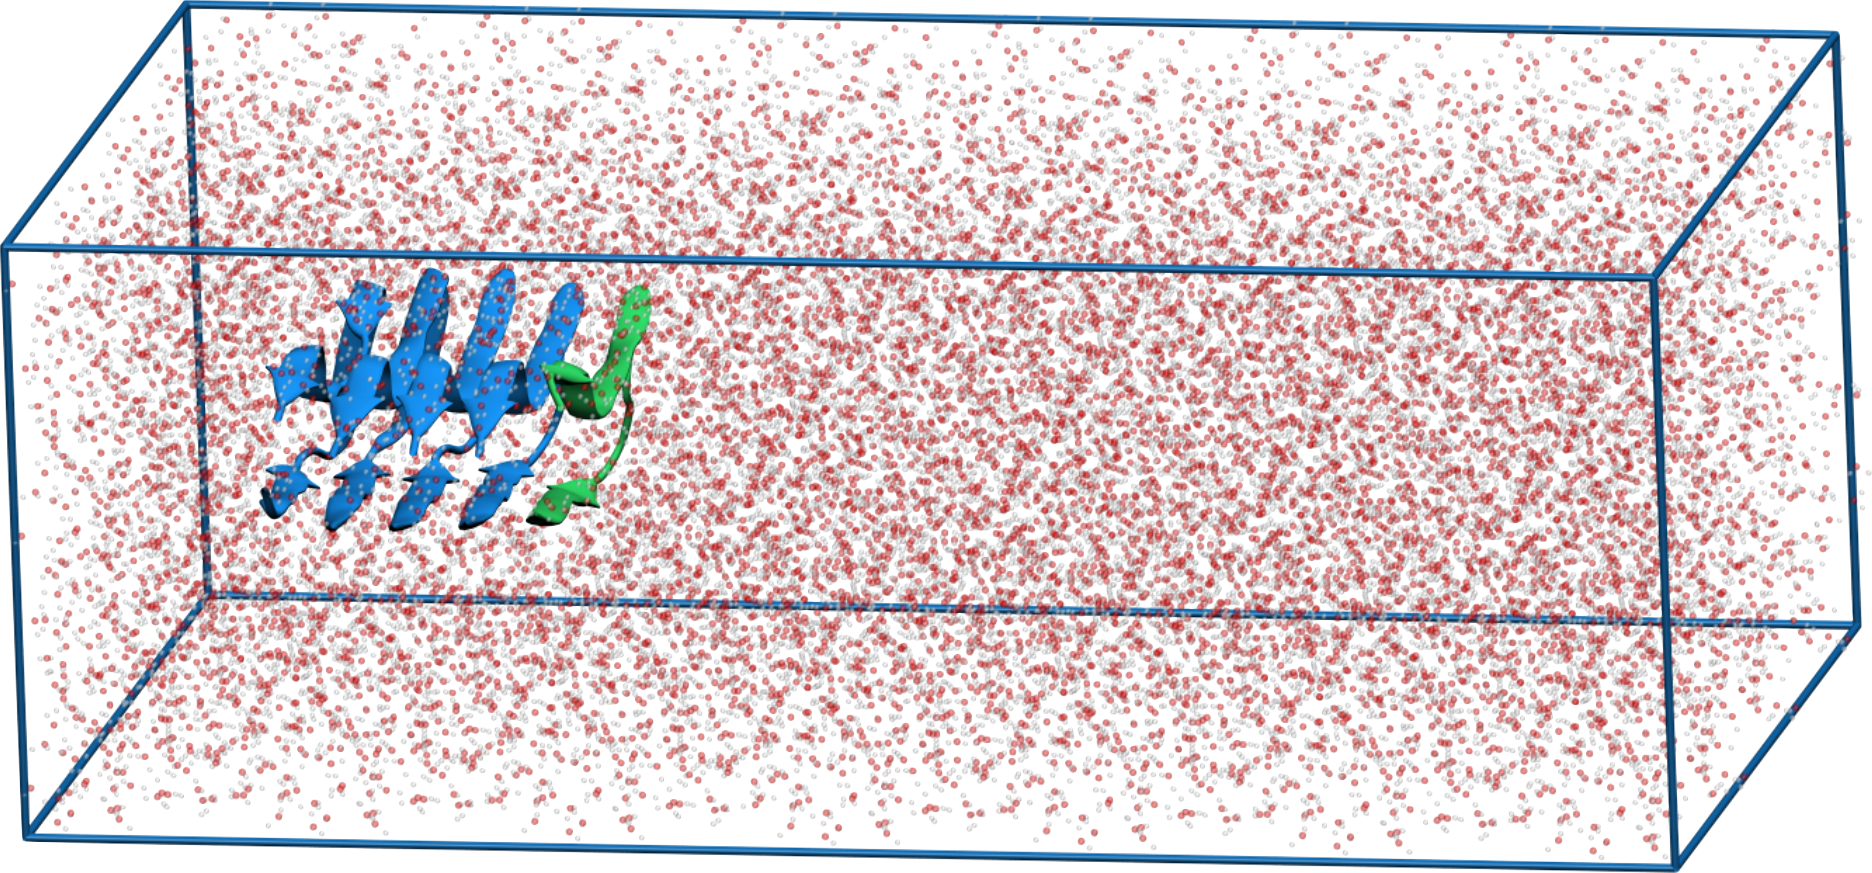
\includegraphics[width=0.48\textwidth]{figures/simbox.png}
   \caption{Example image of what the simulation box should look like for this exercise. The cartoon represents the amyloid, and the color scheme corresponds to \fref{fig:umbrellaSamplingConcept}.}
   \label{fig:simbox}
\end{figure}
Another issue needs to be addressed after the correct simulation box setup. The second chain of the amyloid fibril, \texttt{Chain B}, needs to be fixed in space, which can be realized by positional restraints that restrain each atom to its initial XYZ coordinates. Positional restraints differ from distance restraints because they keep atoms close to absolute reference positions, while distance restraints only restrain coordinates relative to each other. The positional restraints are activated by adding the appropriate lines to the \texttt{topol\_Protein\_chain\_B.itp} file (\code{itp} stands for 'include topology'). The lines to be added are shown below. The keyword \code{POSRES\_B} is critical since the \texttt{MDP} file uses this keyword to implement the positional restraints algorithmically.
\begin{lstlisting}[language=bash]
#ifdef POSRES_B
#include "posre_Protein_chain_B.itp"
#endif
\end{lstlisting}
This last manual step concludes the input file generation. The system must be minimized and equilibrated before a pulling simulation is conducted to obtain configurations along the COM distance coordinate. The \texttt{MDP} files can be downloaded from the online repository and used to execute the commands as usual.
\begin{lstlisting}[language=bash]
gmx grompp -f em.mdp -c solv_ions.gro -p topol.top -o em.tpr
gmx mdrun -v -deffnm em
gmx grompp -f npt.mdp -c em.gro -p topol.top -r em.gro -o npt.tpr
gmx mdrun -deffnm npt
\end{lstlisting}
% PULLING
\begin{figure}
    \centering
    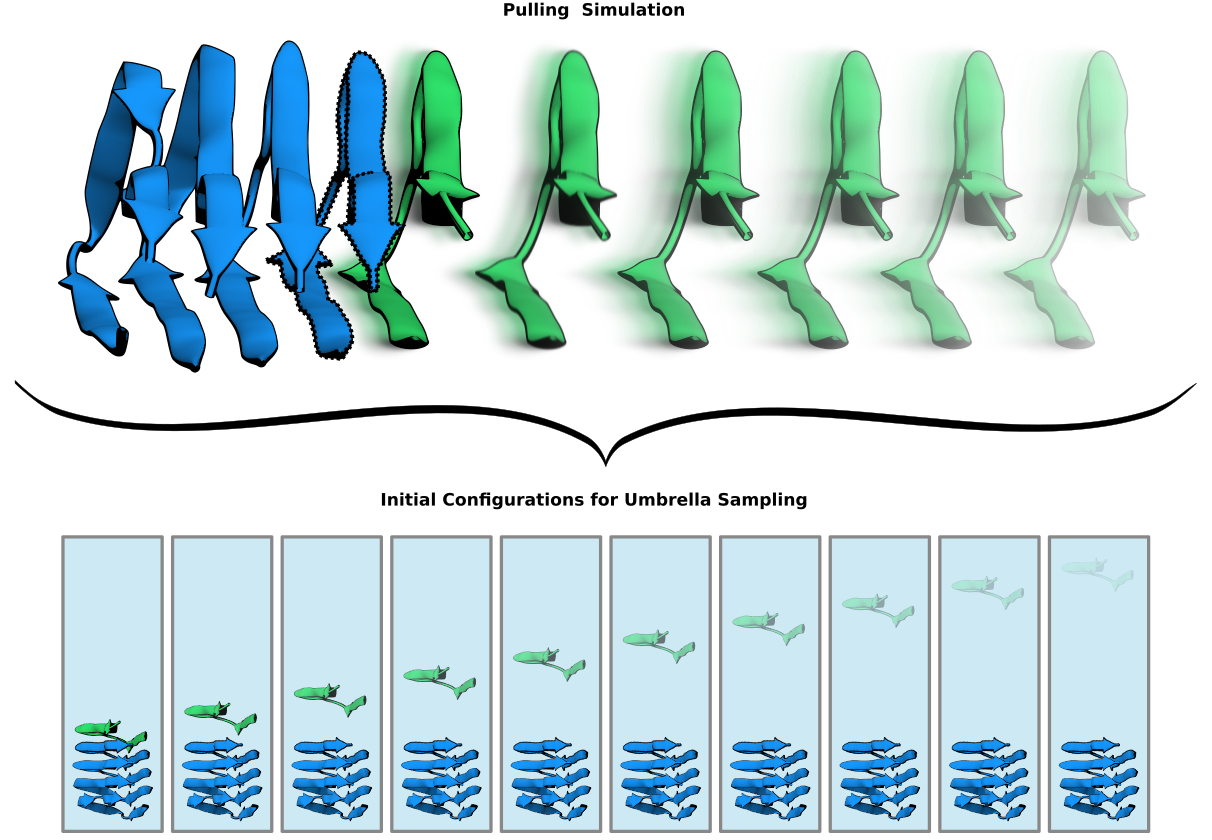
\includegraphics[width=0.48\textwidth]{figures/pulling.png}
    \caption{Concept visualization of the pulling simulation. Along the COM distance coordinate, the outermost peptide (green) is pulled away from the fibril (blue). The second outermost peptide is positionally restraint (pronounced outline). Along the reaction pathway, configurations are saved for the umbrella sampling.}
    \label{fig:pulling}
\end{figure}
The pulling simulation generates configurations to be used as starting frames for the individual umbrella sampling simulations. Thus, \texttt{GROMACS}' pulling functionality is utilized to steer the terminal peptide away from the remaining amyloid fibril in one simulation from which individual snapshots are saved within an approximately linear spacing along the COM distance coordinate (see \fref{fig:pulling}).
For \texttt{GROMACS} to pull a certain atom group, an appropriate index file must be created by the \code{gmx make\_ndx} command that contains the indices of the atom groups to be separated. In this case, the atom groups of the two terminal peptides are saved to the \code{index.ndx} files with the names \code{chain\_A} and \code{chain\_B}. They correspond to the residues one to 27 and 28 to 54. The command \code{gmx make\_ndx} can seem complex for beginners. Therefore, the correct series of commands to generate the index file can be seen below.
\begin{lstlisting}[language=bash]
gmx make_ndx -f npt.gro
...
 > r 1-27
 > name 19 Chain_A
 > r 28-54
 > name 20 Chain_B
 > q
\end{lstlisting}
The validity of \code{index.ndx} can be checked by opening the file via \texttt{VIM} and going to the end of the file (by typing \keystroke{shift} + \keystroke{G}). The non-standard index groups named \code{Chain\_A} and \code{Chain\_B} should be there now. \texttt{GROMACS}' pulling functionality is completely parameterised via the \code{md\_pull.mdp} file (downloadable from the online repository). Below is a brief overview of the keywords that can and must be specified for successful pull simulations in \fref{tab:mdpPulling}. 
\onecolumn
\begin{center}
    \begin{tabularx}{\textwidth}{l X}
    \caption{Tabular description of parameters related to pulling simulations in \texttt{GROMACS}. On the left is the \texttt{MDP}-parameter with its corresponding value, and on the right is a brief description. For further details, refer to the \texttt{GROMACS} manual}\label{tab:mdpPulling}\\
    \toprule
    \texttt{pull = yes}                     & All pull-related keywords are parsed by \code{gmx grompp}. All pull settings are ignored if set to \texttt{no} (default).\\ \midrule 
    \texttt{pull-pbc-ref-prev-step-com = yes} & The reference distance for COM-Pulling is calculated from the periodic boundary state of the prior step. This option is required for newer GROMACS versions with \texttt{pull-group\#-pbcatom}.\\ \midrule
    \texttt{pull\_ngroups = 2}              & Number of pull groups to be steered within the pull simulation. For distance pulling, two groups are required, while an angle would require three groups.\\ \midrule
    \texttt{pull\_ncoords = 1}              & Several pull coordinates can be steered simultaneously (useful for domain unfolding); however, only one pull coordinate is used here.\\ \midrule
    \texttt{pull\_group\#\_name = Chain\_X} & Numbers (\#) and names of the corresponding pull groups as defined in the \code{index.ndx}. Two names must be provided with \texttt{pull\_ngroups = 2} specified in this system. Here: \texttt{Chain\_A} and \texttt{Chain\_B}.\\ \midrule
    \texttt{pull-group\#-pbcatom = 175} & The reference atom of both pull groups for determining the periodic boundary treatment for calculating the COM-distance between the pull groups. The atoms should be located in the center of their respective group. In this case, Atom 175 should fulfill this criterion for both amyloid chains.\\ \midrule
    \texttt{pull\_coord1\_type = umbrella}  & Apply a harmonic potential to the pull coordinate number 1 to significantly limit the phase space accessible to the two pull groups. \\ \midrule
    \texttt{pull\_coord1\_geometry = distance}  & For pull coordinate number 1, apply the harmonic potential to the distance of the two pull groups.\\ \midrule
    \texttt{pull\_coord1\_groups = 1 2} & pull coordinate number 1 should apply to pull groups 1 and 2. This option becomes increasingly important, especially if several groups and coordinates are defined.\\ \midrule
    \texttt{pull\_coord1\_dim = N N Y}  & Apply a bias only in the z-dimension. Thus, x and y are set to "no" (\texttt{N}), and z is set to "yes" \texttt{Y}.\\ \midrule
    \texttt{pull\_coord1\_start = yes}  & the starting value of the pull coordinate number 1 is the value it assumes in the starting configuration.\\ \midrule
    \texttt{pull\_coord1\_rate = 0.01}  & The rate at which pull coordinate number 1 increases in \SI{}{\nano\meter\per\pico\second} over the course of a simulation. If the pull coordinate refers to an angle/dihedral, this rate would be given in \SI{}{\degree\per\pico\second}.\\ \midrule
    \texttt{pull\_coord1\_k = 1000}     & The force constant to parametrize the harmonic potential with, that was set in \texttt{pull\_coord1\_type} in \SI{}{\kilo\joule\per\mole\per\nano\meter^2}. The corresponding variable can be found in \fref{eq:umbrellaBiasingPotential}.\\
    \bottomrule
    \end{tabularx}
\end{center}
\twocolumn
Additionally, \code{md\_pull.mdp} references the statement previously added to the \code{topol\_Protein\_chain\_B.itp} file. The \code{define} keyword at the very beginning uses the same expression to activate the positional restraints of the \texttt{Chain B} (second outermost peptide). Not activating the positional restraints might lead to deformation of the amyloid fibril since the intermolecular interactions between the individual peptides are so strong that individual residues would be towed away together with \texttt{Chain A}.
From the \texttt{MDP} file, it becomes apparent that throughout the \SI{500}{\pico\second} trajectory, the peptide is being pulled \SI{5.0}{\nano\meter} away from the fibril. The keyword \code{nstxtcout}, which is set to \num{500} (every \SI{1}{\pico\second}), determines the frequency for writing out the compressed trajectory to the \texttt{XTC} file. This file will extract the starting configurations for the umbrella sampling. The bash script named \code{02\_simprep.sh} is downloadable from the online repository and automatically takes care of the simulation and frame extraction with a distance spacing of around \SI{0.2}{\nano\meter}. Include a commented version of this bash script as part of the report. Especially the \code{awk} command is quite complex. Nevertheless, any attempts to correctly comment on it are appreciated. Once the run finishes, the success can be tested by plotting the contents of \code{pullf.xvg}, which records the force required over the simulation time. It should look similar to \fref{fig:pullxvg}.
\begin{figure}[H]
    \centering
    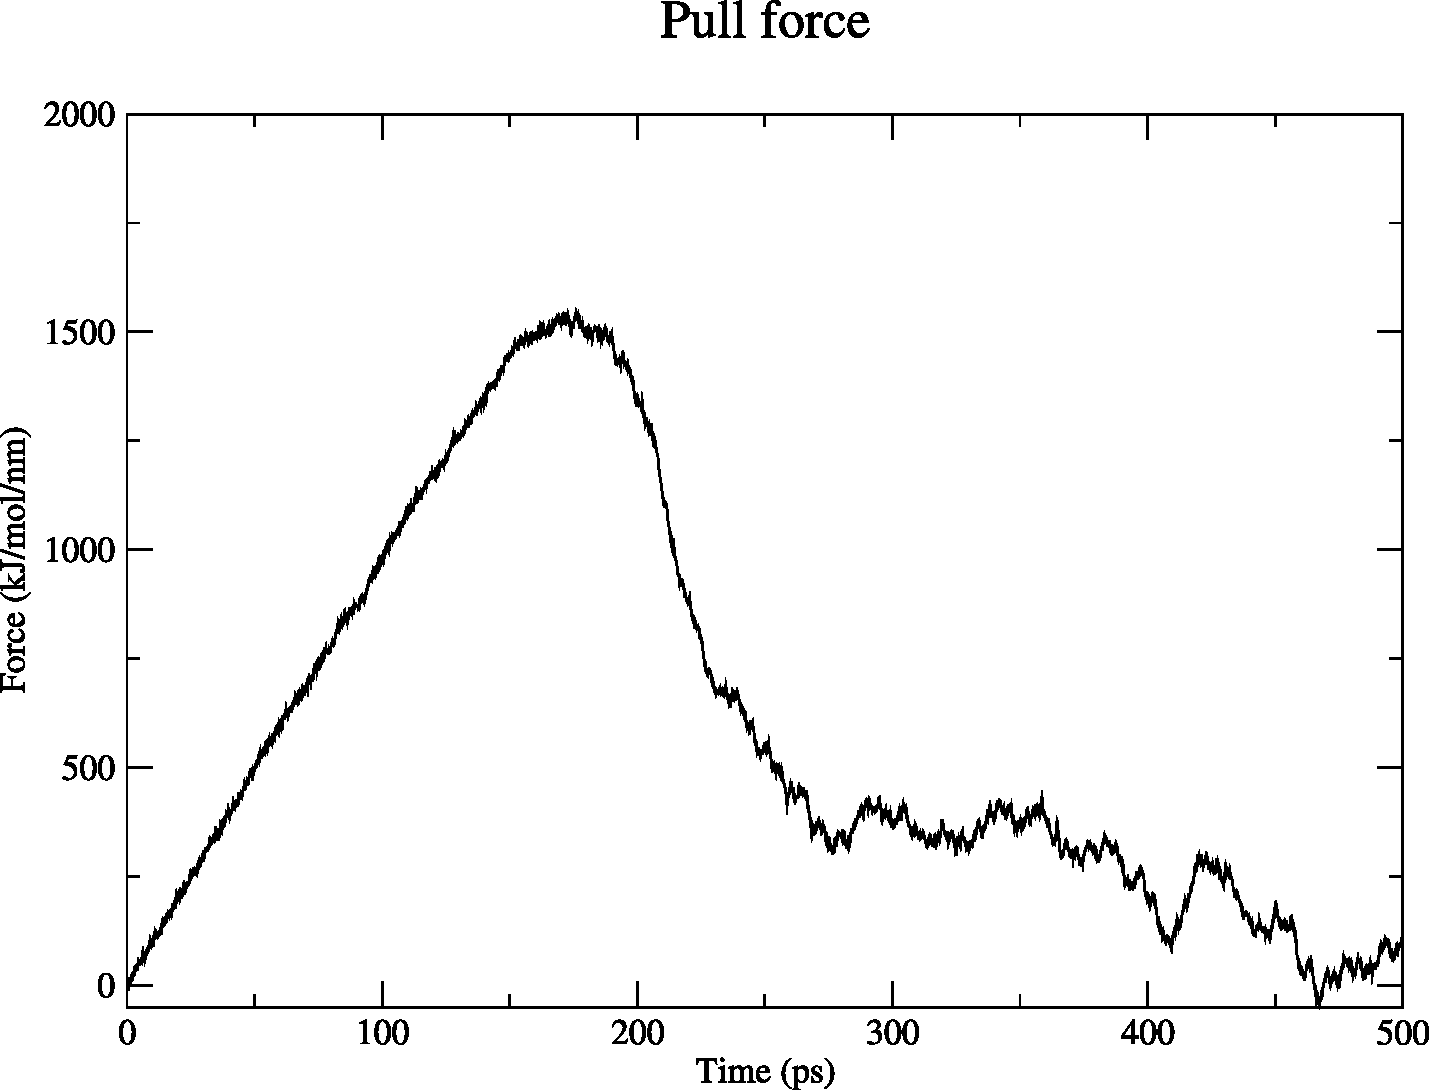
\includegraphics[width=0.48\textwidth]{figures/pullf.pdf}
    \caption{Force on the two pull groups throughout the simulation.}
    \label{fig:pullxvg}
\end{figure}
Apart from the pulling simulation outputs, the script creates two auxiliary files (\code{dist.xvg} and \code{important\_frames.txt}) and a couple of \texttt{GRO} files, e.g., \code{conf191.gro}, that correspond to the frames listed in \code{important\_frames.txt}. These \texttt{GRO} files serve as the starting configurations for the umbrella windows. The \SI{0.2}{\nano\meter} spacing can be verified by comparing the frames listed \code{important\_frames.txt} with their corresponding distances in \code{dist.xvg}.\\
The umbrella sampling simulations rely on the same \texttt{GROMACS} parameters as the pull run. Comparing \code{md\_pull.mdp} with \code{md\_umbrella.mdp} or \code{npt\_umbrella.mdp} reveals that only the \code{pull\_coord1\_rate} differs by being set to zero for the umbrella sampling. Thus, the molecules are not actively pulled apart; a harmonic potential keeps the distance constant to its initial value. Each starting frame extracted by \code{02\_simprep} requires a quick NPT equilibration followed by a production run over \SI{500}{\pico\second}. The individual simulations are sometimes referred to as umbrella windows. A code example for executing the runs can be found below. 
\begin{lstlisting}[language=bash]
gmx grompp -f npt_umbrella.mdp -c conf<f>.gro -p topol.top -r conf<f>.gro -n index.ndx -o npt<f>.tpr
gmx mdrun -v -deffnm npt<f>
gmx grompp -f md_umbrella.mdp -c npt<f>.gro -t npt<f>.cpt -p topol.top -r npt<f>.gro -n index.ndx -o umbrella<f>.tpr
gmx mdrun -v -deffnm umbrella<f>
\end{lstlisting}
Creating a bash script to automate the simulation runs is highly recommended.\\


\subsection*{Analysis}
With the umbrella sampling successfully conducted, the equilibrated data can be analyzed. Usually, $\Delta G_\text{\tiny bind}$ is calculated from the free energy surface (FES) obtained from MBAR or WHAM. The convenient \code{gmx wham} tool already implemented in \texttt{GROMACS} is showcased herein.\cite{Grossfield_WHAM} The value of $\Delta G_\text{\tiny bind}$ is simply the difference between the highest and lowest values of the FES (see \fref{fig:GofXiAnnotated}), as long as the values of the FES converge to a plateau at large COM distances. It represents the potential of mean force (PMF) to separate the terminal peptide from the tip of the protofilament.\\
The input to be fed into \code{gmx wham} consists of two files to be created by the user. The first one contains line-wise entries of all \texttt{TPR} file names corresponding to the umbrella windows, and the other file includes the names of the \code{pullf.xvg} or \code{pullx.xvg} files, respectively. These lists could be called, e.g., \code{tpr-files.dat}; the contents are listed below for illustration.
\begin{lstlisting}[language=bash]
umbrella45.tpr
umbrella123.tpr
...
umbrella487.tpr
\end{lstlisting}
Conducting the analysis is relatively simple since it only requires the user to execute the correct \texttt{GROMACS} command.
\begin{lstlisting}[language=bash]
gmx wham -it tpr-files.dat -if pullf-files.dat -o -hist -unit kCal
\end{lstlisting}
The WHAM module opens each of the \code{umbrella*.tpr} and \code{umbrella*\_pullf.xvg} files and runs the WHAM analysis on them. This program outputs two essential files named \code{histo.xvg} and \code{profile.xvg}, which contain the histogram data and the resulting FES profile against the COM distance coordinate. They can be visualized using \code{xmgrace}.
\begin{lstlisting}[language=bash]
xmgrace profile.xvg
xmgrace -nxy histo.xvg
\end{lstlisting}
As exemplary results, a FES is shown in \fref{fig:expectedResults}. The difference from the highest to the lowest point of this FES according to \fref{eq:deltaGbind} yields a $\Delta G_\text{\tiny bind}$ of around \SI{-37}{\kcalm}. The difference to the published value of \SI{-50.5}{\kcalm} is quite significant; however, there are also artifacts visible in the FES around \SIlist{1;1.5;3.5;4.3}{\nano\meter} that result from insufficient histogram overlap.
% Expected outcome
\begin{figure}[H]
    \centering
    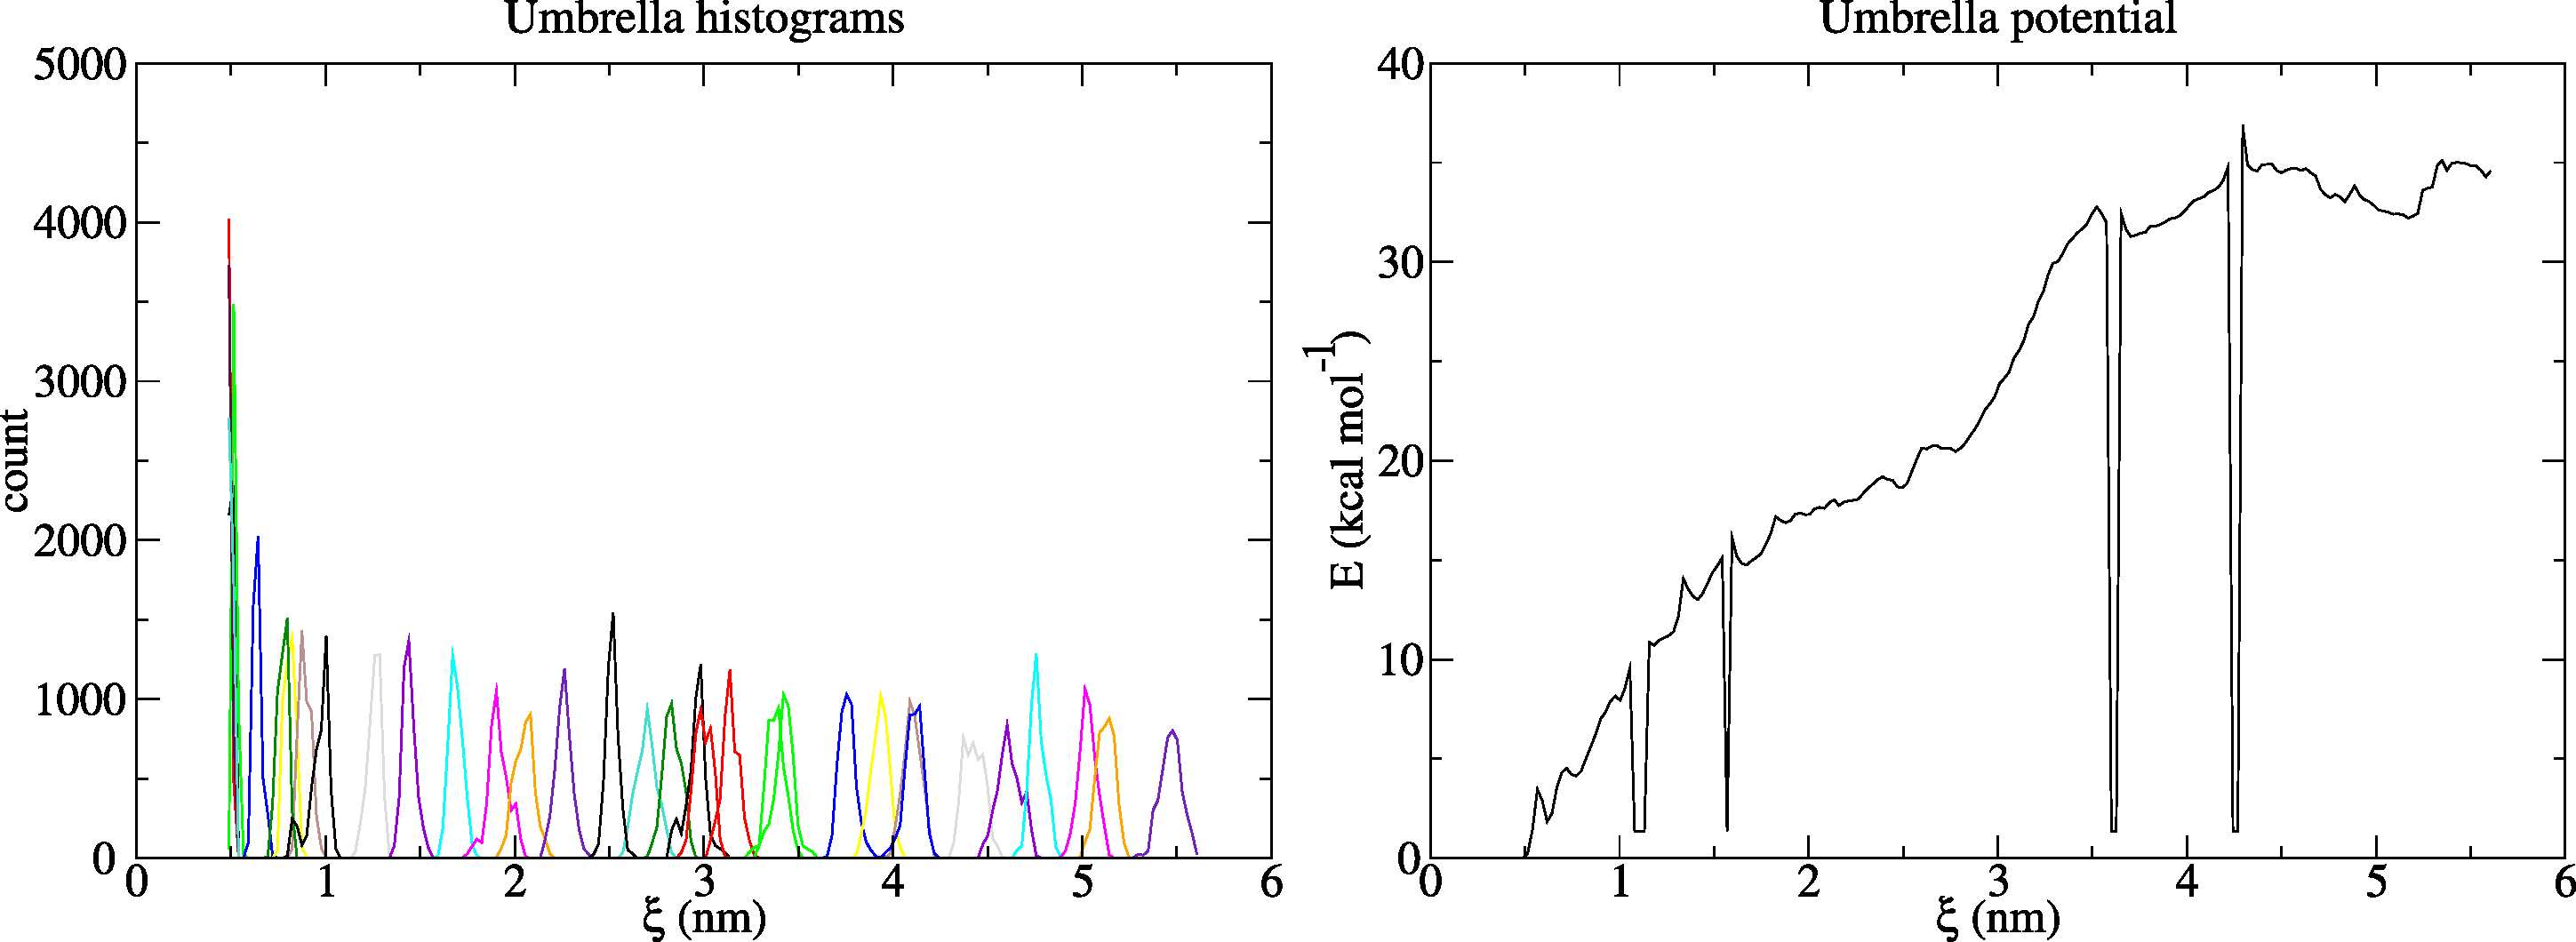
\includegraphics[width=0.48\textwidth]{figures/expectedResults.pdf}
    \caption{Distance probability distributions (histograms) for the different windows (left) and the corresponding FES along the COM distance coordinate (right).}
    \label{fig:expectedResults}
\end{figure}
Since each umbrella window is independent, these artifacts can be solved by post-sampling the missing distance histograms. Inserting new umbrella simulations with starting configurations centered on the defective region should mitigate the inaccuracy. The file \code{dist.xvg} contains frames on the first column and distance on the second column so that the correct snapshot to start a post-sampling simulation can be found. Once the desired frame is known, equilibration and production simulation can be conducted, and \texttt{TPR} and \texttt{XVG} files are added to \code{tpr-files.dat} and \code{pullx-files.dat}. Repeating the WHAM analysis should result in an FES that has fewer defects. An exemplary FES that contains no artifacts anymore after successful post-sampling is shown in \fref{fig:expectedResults_combined}. Here, $\Delta G_\text{\tiny bind}$ is obtained with \SI{40}{\kcalm}, which is better than before but still deviates with 20\% from the literature value. There are many tools for quality control and optimization of free energy calculations\cite{Klimovich_2015}, but for educational purposes, such a value is more than sufficient.
\begin{figure}[H]
    \centering
    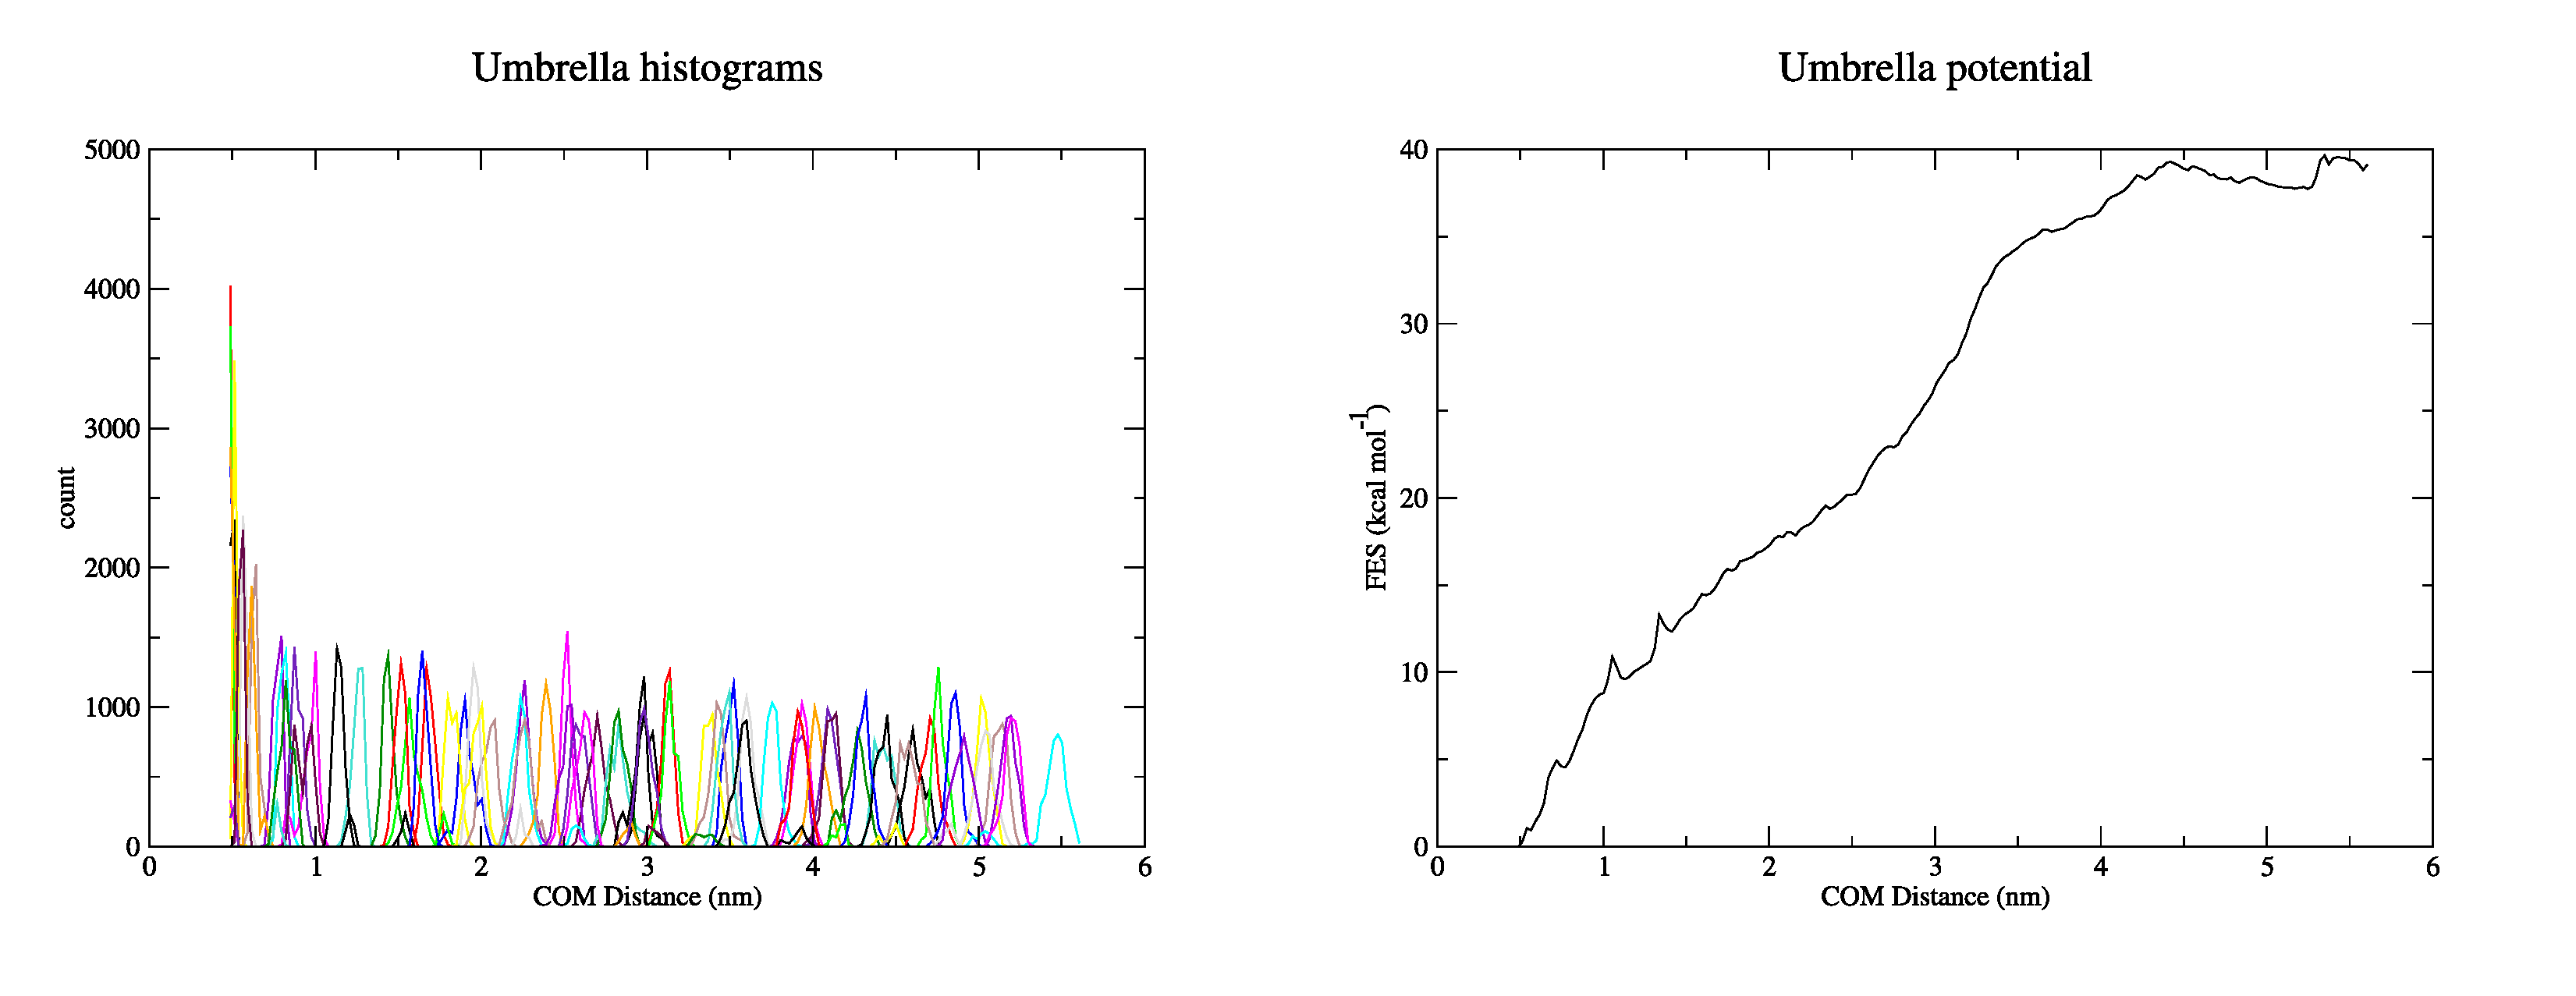
\includegraphics[width=0.48\textwidth]{figures/expectedResults_combined.pdf}
    \caption{Free-energy profile (FES) along the reaction coordinate {\textxi} (top panel) and corresponding distance probability distributions (histograms) for the different windows (bottom panel).}
    \label{fig:expectedResults_combined}
\end{figure}
The report should include the histograms and the FES as plots, as well as the value obtained for $\Delta G_\text{\tiny bind}$. A brief discussion of the plots and a comparison with the literature value should be included. Post-sampling is optional but recommended. Eventually, the FES, and thus the free energy estimate, can be further enhanced by collaborating with other users or students to collect as many \texttt{TPR} and \texttt{PULL} files as possible. After adjusting \code{tpr-files.dat} and \code{pullx-files.dat} (or \code{pullf-files.dat}), WHAM would analyze a vast amount of data, which could close the gap to the literature value.

\newpage

\section{Exercise 8: Protein Simulation with Convergence and Principal Component Analysis}\label{sec:ProteinSim}
\begin{Checklists}
    \begin{checklist}{Tasks for the Eighth Exercise}
    \textbf{Finish these tasks and write a short report about your findings.}
    \begin{itemize}
		\item Write a Methods section describing your MD simulation setup.
		\item Monitor and report stability measures for the pre-production step of the simulation setup for Potential energy (EM), temperature (NVT), density, and pressure (NPT). 
		\item Conduct a BSE analysis for $R_\text{gyr}$ and RMSD(t) of your production run. Use the crystal structure as a reference and discuss the results with respect to sampling quality. 
		\item Show the two extreme projections of the eigenvectors. Also, include a plot of the atomic contributions of eigenvectors 1-10 with a brief discussion.
		\item Plot PC1 vs PC2, PC1 vs PC10 and PC9 vs PC10 and discuss the plots briefly.
	\end{itemize} 
    \end{checklist}
\end{Checklists}
\begin{figure}[H]
    \centering
    \includegraphics[width=0.45\textwidth]{figures/5yok_water_render.png}
    \caption{HIV-protease in a water box.}
    \label{fig:5yok_water_render}
\end{figure}


\subsection*{Introduction}
In this exercise, the user conducts an equilibrium molecular dynamics (MD) simulation for the protein HIV-protease (PBD: 5YOK). As a novelty, the simulation setup in this exercise will be self-supervised. The methods applied in the prior exercises can be used as a template library and to draw inspiration. Furthermore, this exercise is concerned with the convergence of the simulation with respect to the protein conformation for which a blocked standard error (BSE) analysis\cite{Grossfield_2009} will be conducted. Finally, the movements of the HIV-protease are of utmost importance due to their influence on reducing drug efficacy. The principal component analysis (PCA) will illuminate the global molecular movement of this drug-resistant variant.\cite{Yang_2008}


\subsection{Theoretical Considerations}
\subsubsection*{Accessing Sampling Quality and Convergence}
Convergence in a simulation is achieved once additional sampling does not change an obtained result significantly. This definition aligns with the concept of relative convergence, which describes statistical uncertainty concerning an observable. While absolute convergence cannot be ensured or estimated in an MD simulation, relative convergence has been the subject of extensive studies, and one method to access the relative sampling quality is to conduct a blocked standard error analysis for an observable.\cite{Grossfield_2009}\\
\begin{figure}[H]
    \centering
    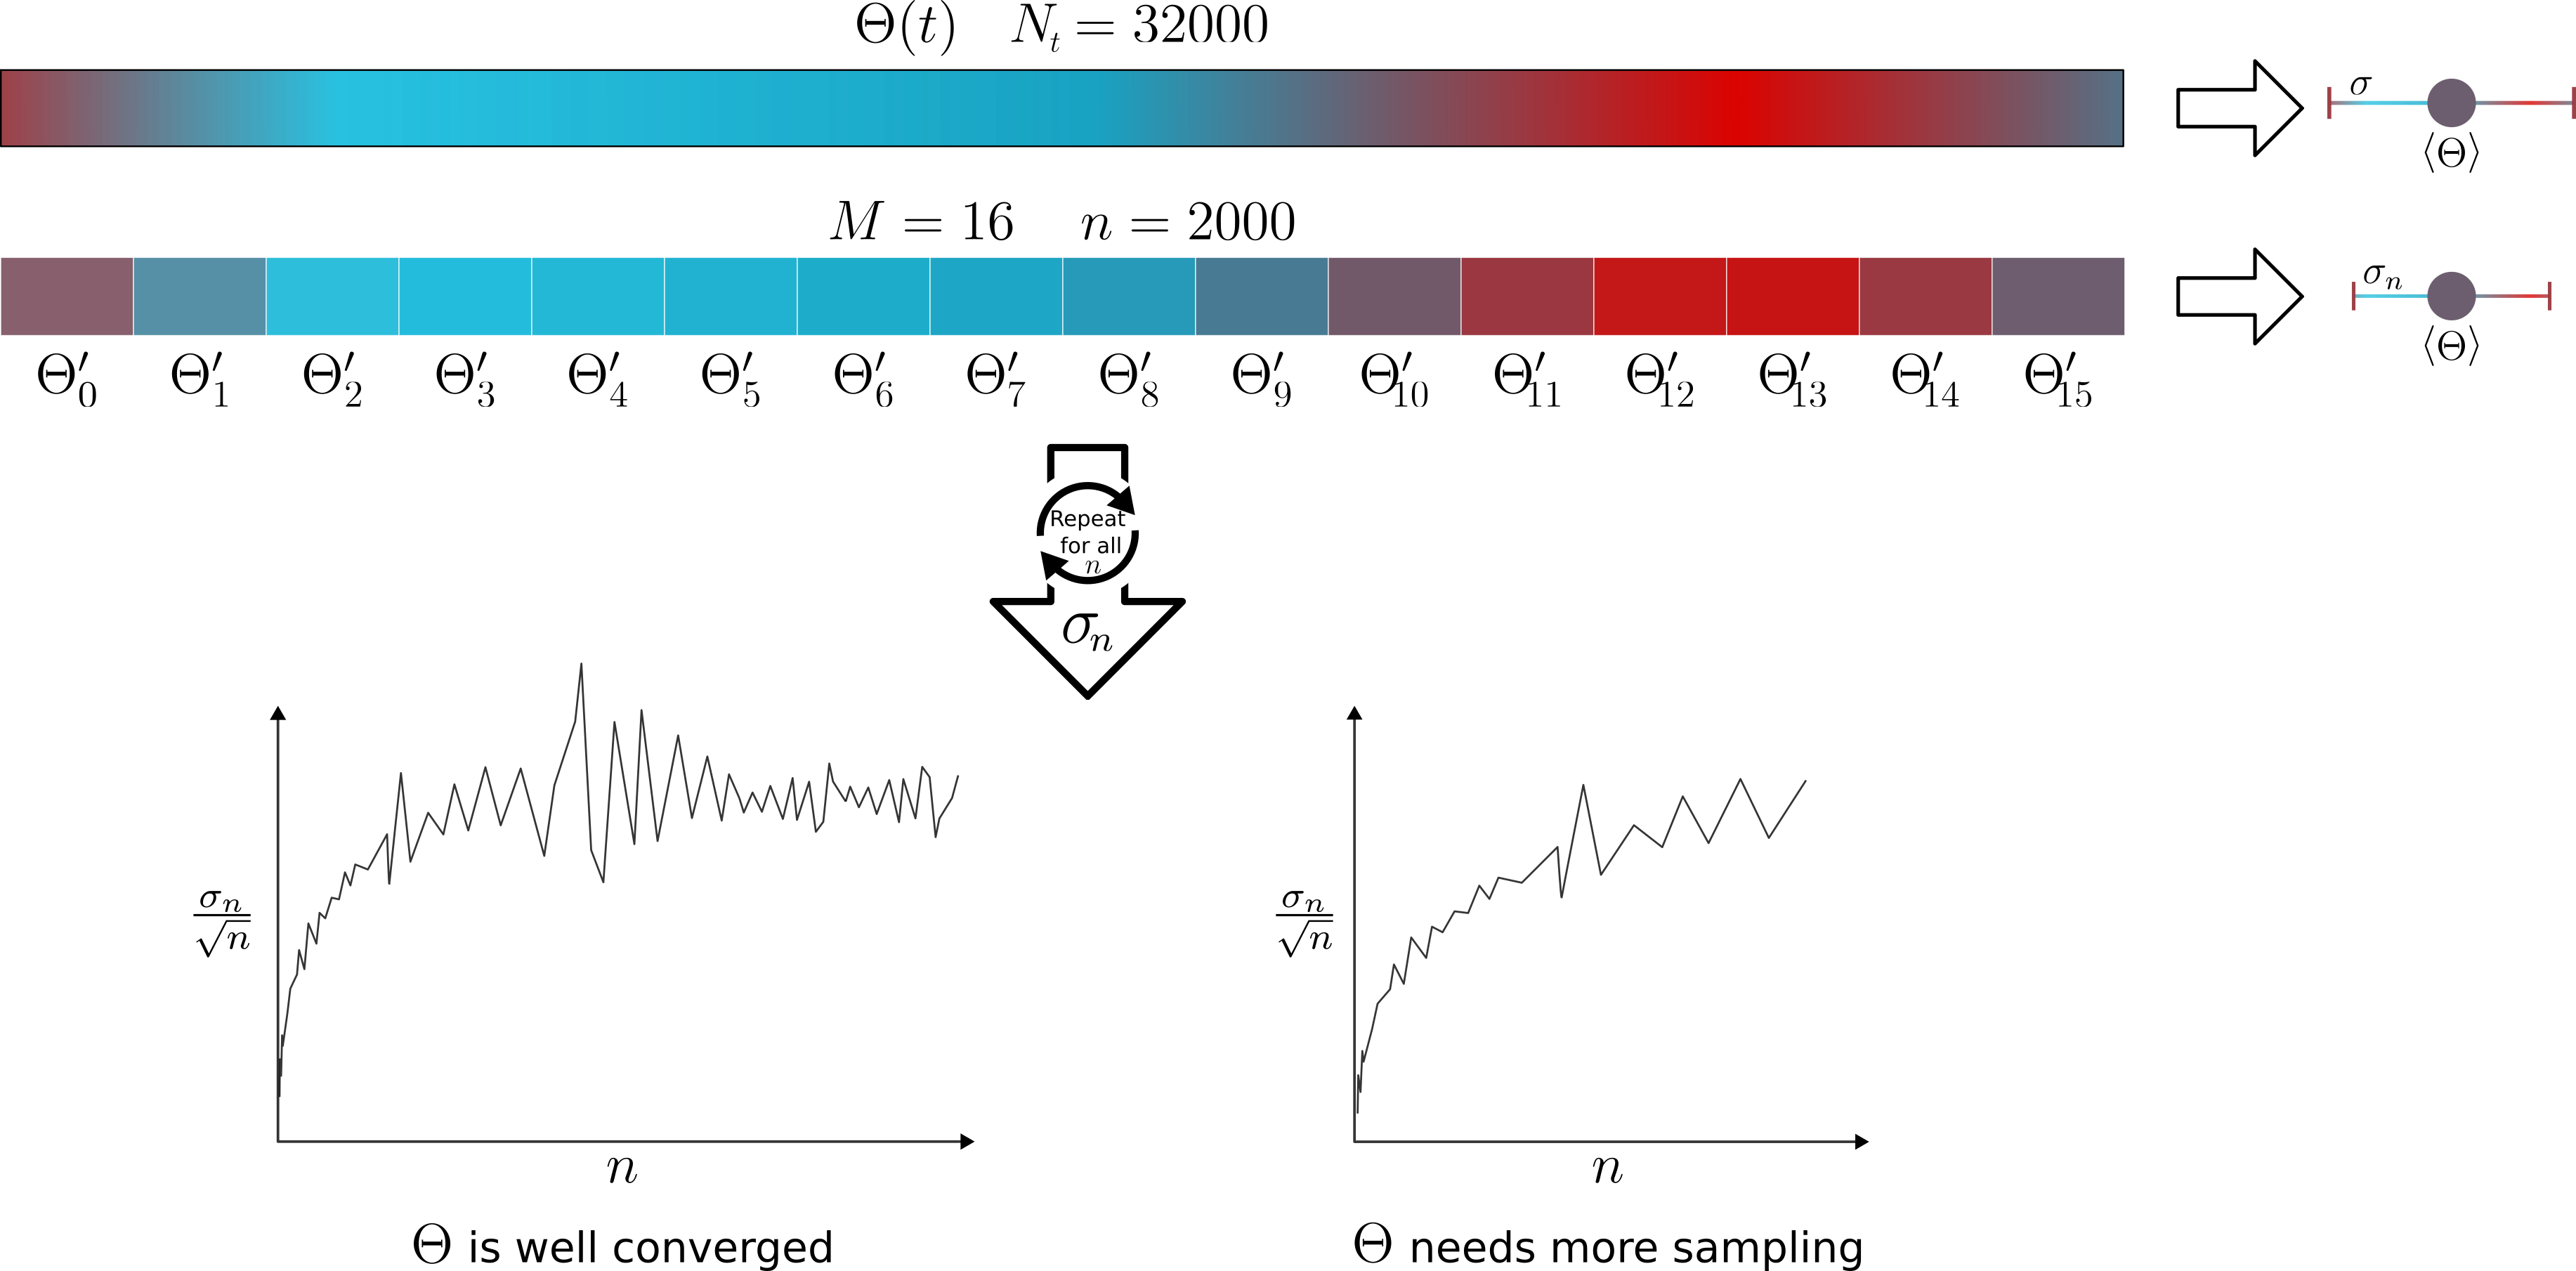
\includegraphics[width=0.45\textwidth]{figures/bse_concept.png}
    \caption{Concept of the analysis of block averages. When evaluated on a whole trajectory, an observable $\Theta$ yields average $\langle \Theta \rangle$ and standard deviation $\sigma$. The color indicates some arbitrary magnitude of the instantaneous quantity $\Theta$. Let the total sample size be 32000, i.e., 32000 instantaneous values of $\Theta$ have been collected. Splitting the trajectory into $M$ blocks, with $n$ data points each, and then calculating each block's average yields the same overall average. However, the standard deviation of the block averages is different, $\sigma_n \neq \sigma$. Repeating this process for all possible $M$,$n$ pairs produces a curve that indicates convergence for $\Theta$.\cite{Grossfield_2009}}
    \label{fig:bseconcept}
\end{figure}
% BSE Theory
For $\Theta$, statistical relevancy is only achieved once enough independent samples can be measured. Thus, measuring 30 consecutive frames of a slow movement will result in a sharply defined average value. However, it is not significant since the measurements can be assumed to be highly correlated. Correlated data is invalid for the application of the central limit theory, which states that for measuring infinitely many independent random variables, a normal distribution emerges. The BSE analysis transforms the initial, correlated observations of $\Theta$ by splitting the trajectory into $M$ blocks $m$, each length $n$, and calculating the average of each block $m$, $\Theta^\prime_m$. From the $M$ obtained values $\Theta^\prime_m$, the $n$-specific standard deviation is calculated.
\begin{align}
    \sigma_n & = \sqrt{\frac{1}{M-1} \sum_{m=0}^M  \left( \Theta^\prime_m - \langle \Theta \rangle \right)^2}
\end{align}
At some point, by increasing $n$, the correlation time for $\Theta$ is exceeded, rendering $\Theta^\prime_m$ effectively uncorrelated, which yields a normal distribution $\mathcal{N}$ with fixed mean and variance, given a large enough sampling size.\cite{Flyvbjerg_1989}
\begin{align}
    \lim_{M\rightarrow\infty} \Theta^\prime_m \sim \mathcal{N}\left(\mu,\frac{\sigma_n}{\sqrt{n}}\right)
\end{align}
Since $\sigma_n/\sqrt{n}$ resembles $\sigma$ of the stable normal distribution, plotting it against the "time period'' (i.e., block size $n$) used for block averaging, results in a horizontal plateau, but only if the samples are truly uncorrelated. For smaller values of $n$ where $\Theta^\prime_m$ is still correlated, the corresponding $\sigma$ will steeply approach the stable standard error.\\
\subsubsection*{Principal Component Analysis of Atomic Movements}
The Principal Component Analysis (PCA) is a two-step process that begins by calculating the covariance matrix of the atomic movements in the trajectory. An eigenvector decomposition is then performed on this matrix, resulting in $3N$ eigenvectors (principal components) and associated eigenvalues.
The eigenvectors define the principal motions of the protein. These eigenvectors are typically sorted from highest to lowest eigenvalue, representing the largest and smallest protein motions, respectively. The higher principal components exhibit a higher degree of collectivity, meaning that a small number of high-level principal components account for the essential protein movement, which can provide insights into crucial functionalities.\cite{David_2013}\\
Mathematically, principal components are a set of new variables which are just linear combinations of the initial input variables. In the present description, the input variables are the atom coordinates. The coefficients of the linear combination are chosen so that the resulting principal components are uncorrelated, i.e., they carry independent information. The eigenvectors then denote the directions of largest variance or fluctuations (i.e., \textit{information}) in the data, and the eigenvalues denote the amount of variance in each principal component.  


\subsection*{Setup and Simulations}
This time, the setup of the MD simulations is self-designed. Temperature, pressure, concentration, and other specifics should be reasonably close to physiological or laboratory conditions, as in the preceding exercises. 
If prior exercises are plundered for \texttt{MDP} files, it is advised to reevaluate the parameters e.g. by comparing them to parameters of another MDP file or by checking against the \texttt{GROMACS} \texttt{MDP} options (\url{https://manual.gromacs.org/2024.4/user-guide/mdp-options.html}). Furthermore, the protein should not interact with its closest image; however, making the box dimensions too big would result in longer simulations due to excess water molecules. Therefore, the simulation design should be planned carefully. The water model and forcefield must be chosen as well. Technically, there has to be empirical evidence for the successful interplay of the forcefield and water model. However, since this is out of the scope of this exercise, mixing any options is allowed. However, the rule of thumb is that new is always better.\\
The report should contain a section describing the essential choices and parameters for the MD simulation, similar to how it is done for scientific publications. There are no strict conventions, but a good orientation is to describe the design in a way that is similar to the computational process of setting the system up. Thus, a reasonable order would be the system and source of the initial coordinates, force, field, solvent and box, equilibration, and production. For the latter two, each stage should at least contain information about thermo- and barostat, as well as electrostatics treatment and simulation time. Furthermore, it is good practice to mention constraints that are applied to any bonds. Of course, any information that seems relevant may be reported additionally. For guidance, the method section of any publication utilizing MD simulations can be referred to.\\
Furthermore, the stability of the equilibrations must be ensured and shall, therefore, be included in the report. Energy minimization optimizes potential energy, and plotting it against minimization steps should lead to a curve that converges on a minimal potential energy value. As shown in prior exercises, the canonical ensemble (NVT) keeps the temperature constant under certain fluctuations. Hence, the temperature should be measured for this equilibration step. The last part of the equilibration uses the isothermic-isobaric ensemble (NPT) that keeps the pressure constant. Since the pressure fluctuates quite strongly, the time evolution of the density would be of interest. For the report, one of these plots can be chosen and should be included as an indicator of the simulation stability. As a last remark, it should be mentioned that the \texttt{PDB} file contains non-standard compounds, which are not parametrized in the present forcefields. Thus, they must be deleted before building the simulation system (\texttt{PyMOL} or \texttt{VIM} is recommended). 

\subsection{Analysis}
After successful simulation, the user shall perform a blocked standard error analysis with \texttt{GROMACS} which is relatively easy. When using \code{gmx analyze} the flag for error estimation, \code{-ee} needs to be specified. As an input, the command takes an \texttt{XVG} file, e.g., some file created by \code{gmx rms}. The commands to generate the BSE analysis for the RMSD and $R_\text{gyr}$ could look like the following:
\begin{lstlisting}[language=bash]
gmx trjconv -s prod.tpr -f prod.xtc -o prod_center.xtc -pbc mol -center
gmx gyrate -f prod_center.xtc -s prod.tpr -o rgyr.xvg
gmx rms -s em.tpr -f prod_center.xtc -o rmsd.xvg
gmx analyze -f rmsd.xvg -ee bse_rmsd.xvg
gmx analyze -f rgyr.xvg -ee bse_rgyr.xvg
\end{lstlisting}
The two plots should be part of the report. In order to quantify statistical significance from the BSE plot, some intuition is necessary since the convergence onto a horizontal line is only achieved in an ideal setup. Therefore, it needs to be discussed whether the amount of sampling is enough.\\
Furthermore, a PCA shall be conducted with an eigenvector analysis. \texttt{GROMACS} provides powerful tools to analyze the principal components of a trajectory, which can aid in understanding the functioning of HIV-protease. Calculating the eigenvectors from the trajectories can be done by the following lines of code:
\begin{lstlisting}[language=bash]
gmx covar -f prod_center.xtc -s prod.tpr -xpma
\end{lstlisting}
This command also produces the covariance matrix, eigenvectors, and eigenvalues by default. This information about the principal motions can be further processed by \code{gmx anaeig} to visualize different properties concerning atomic motion and convergence. The atom-wise component for each principal component is specified via the \code{-comp} flag, and the eigenvector projections on the trajectory with the \code{-proj} flag.
\begin{lstlisting}[language=bash]
gmx_mpi anaeig -v eigenvec.trr -f prod_center.xtc -s prod.tpr -proj eigproj1_10.xvg -comp eigcomp1_10.xvg -last 10 
\end{lstlisting}
The atomic components are difficult to rationalize since each atom contributes only a small amount to each principal component. Nevertheless, important information might be deducted, especially for the collective high-level principal components. The projection on the trajectory can give some clues concerning the convergence of the trajectory, albeit the information is of a qualitative nature. Given the first two principal components, which are highly collective but decorrelated motions, different sampling spaces or clusters can be identified if their trajectory projections are plotted against each other. In a well-sampled simulation, each of these clusters should show a variety of transitions. Thus, in an insufficiently sampled simulation, each cluster is sparsely populated with only a few transitions.\\
Since most of the atomic motion is captured in the higher principal components, it should be enough to calculate the projections and atomic components for the first \num{10} eigenvectors. The plots of the atomic components of all \num{10} eigenvectors should be included in the report with a very brief discussion. This plot is generated directly from the \code{gmx anaeig} output as an \texttt{XVG} file. The trajectory projections, however, require manual postprocessing since the corresponding \texttt{XVG} file lists the principal component against time information. In order to assess the sampling quality, the report should include a plot of PC1 against PC2. Additionally, plots of PC1 against PC10 and PC9 against PC10 are necessary to visualize the decreasing importance of lower eigenvectors. Discuss the plots' convergence and rationalize the usage of PC1 vs. PC2 for quality assessment over any other PC pair. Exemplary plots can be seen in \fref{fig:expca}.\\
Another useful flag of \code{gmx anaeig} is the \code{-extr}, which yields the two extreme states of the largest eigenvector. Visualizing them conveys an idea about the largest collective motion of the system, and the \texttt{PDB} structures that correspond to the end-states can be generated with the following command.
\begin{lstlisting}[language=bash]
gmx anaeig -v eigenvec.trr -f prod_center.xtc -s prod.tpr -extr
\end{lstlisting}
It is recommended to visualize the end-states in VMD instead of \texttt{PyMOL} and to include snapshots in the report. Choosing a representation and a view that supplements a brief discussion is beneficial. Knowledge about binding sites and other structural features should be incorporated.
\begin{figure}[H]
    \centering
    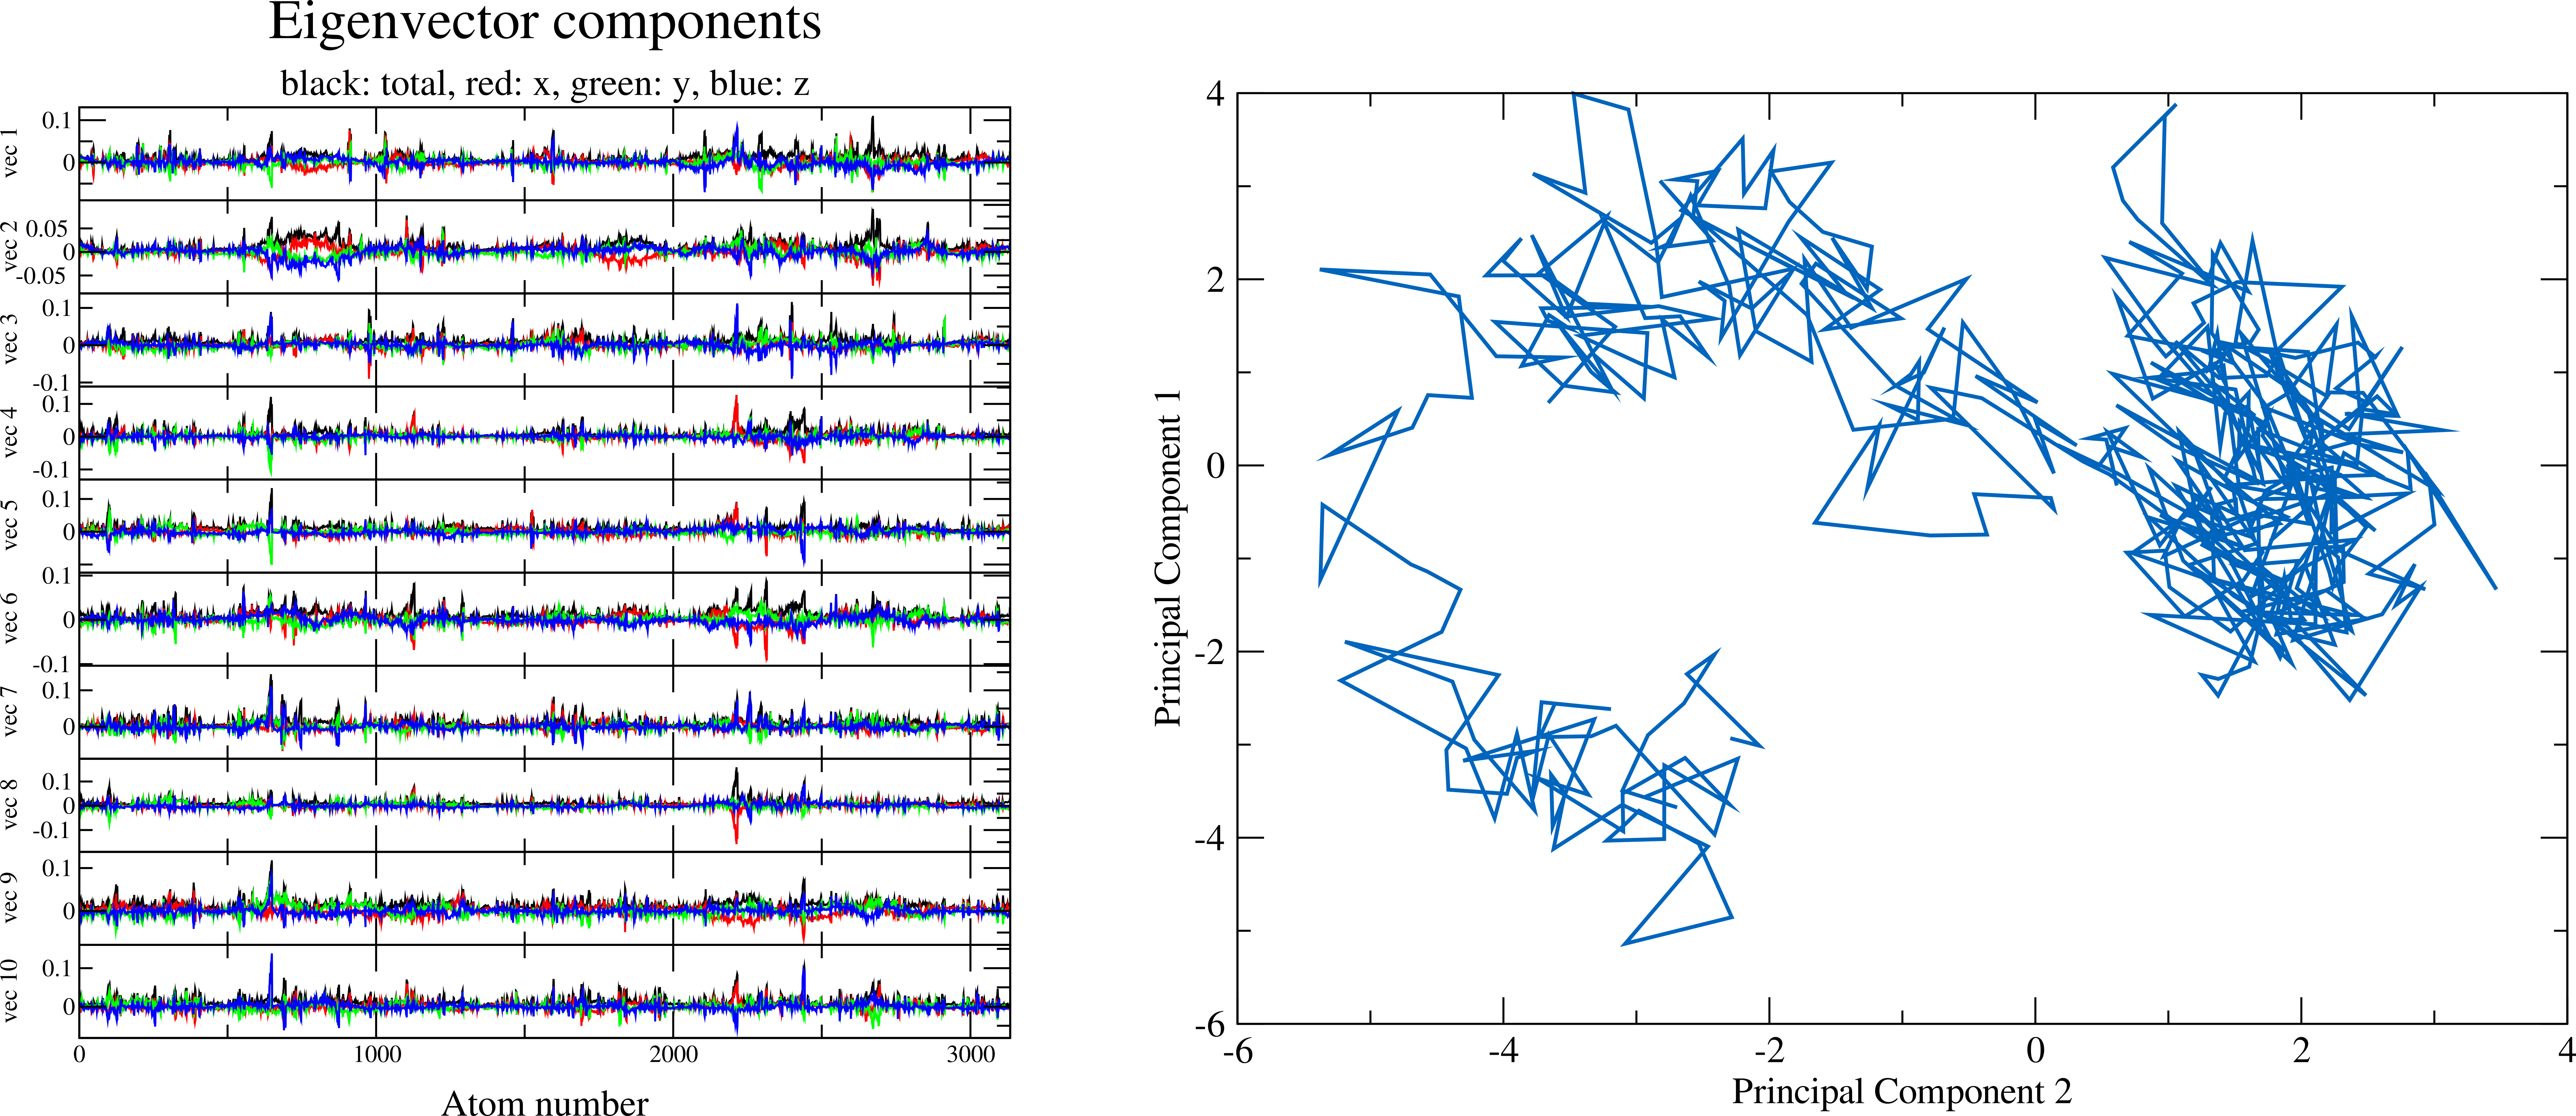
\includegraphics[width=0.45\textwidth]{figures/pca_examples.png}
    \caption{Exemplary results of the atomic components of the first ten eigenvectors and the trajectory projections. The atomic components indicate which atoms contribute to which global movement of the protein. The plot of the principal components 1 and 2 reveals that some clusters along the pathway are sparsely sampled.}
    \label{fig:expca}
\end{figure}

\newpage

\section{Exercise 9: Virtual Drug Screening and MM/GBSA}\label{sec:CompDrugDesign}
\begin{Checklists}
    \begin{checklist}{Tasks for the Ninth Exercise}
    \textbf{Finish these tasks and write a short report about your findings.}
    \begin{itemize}
		\item Try to complete each of the steps of this exercise
		\item At the end of this exercise, suggest 1-2 chemical compounds as potential protein-protein-interaction stabilizers for the receptor complex at hand.
		\item Discuss the suggested compounds and explain why these compounds seem promising. Use the plots and measurements in the respective steps to support your reasoning.
		\item In case the exercise could not be finished, describe any problems you encountered as detailed as possible. Also, document your troubleshooting attempts.
	\end{itemize} 
    \end{checklist}
\end{Checklists}
\begin{figure}[H]
    \centering
    \includegraphics[width=0.48\textwidth]{figures/PPIS_cover.png}
    \caption{Concept art of protein-protein interaction stabilizers. At the interface of the depicted protein complex (green and blue macromolecules) small organic molecules can bind to fasten the connection between the complex sub-units. The small organic molecules would then act as molecular glue.}
    \label{fig:PPIS_cover}
\end{figure}

% Preliminaries and Installations
\subsection*{Introduction}
Typically, drug design focuses on finding a drug (ligand) that binds to a given drug target (i.e. the receptor/protein/complex). The binding occurs at a specific location on the receptor known as the binding pocket. Thus, three objects are required for a drug-discovery endeavour: the receptor, a pocket, and a ligand. Each receptor has multiple available pockets, and many compounds can fit into each pocket. The workflow itself consists of five different steps. Firstly, (1) a protein system must be chosen and pre-processed for subsequent computer-assisted tasks, i.e., its \texttt{PDB} file. After that, (2) a potentially druggable pocket in the protein must be found. Pocket detection is followed by (3) compiling a database of possible compounds in a process called virtual screening. Filtering this database for the best compound (4) is achieved by molecular docking, which evaluates the possible poses of a ligand in a given binding pocket and ranks them according to favourable receptor-ligand interactions, referred to as scoring. For example, a drug candidate that forms many hydrogen bonds with the receptor will have a high docking score. Finally, (5) promising drug-receptor complexes can be further investigated via molecular dynamics simulations and binding free-energy calculations. Apart from a favourable binding free energy, a viable drug candidate must also fulfil several other criteria: it must be non-toxic, selectively bind to the target without affecting other proteins, be administrable, and be feasible to synthesize.\\ 
Protein-protein interactions play pivotal roles in various biological processes, and their perturbation is associated with a wide range of diseases. Consequently, targeting these interactions presents a valuable therapeutic strategy. This exercise focuses on a novel class of drugs known as protein-protein interaction modulators, specifically protein-protein interaction stabilizers. These stabilizers are designed to strengthen the interactions between two proteins forming a complex. The goal is to identify a drug-binding pocket at the interface of the two proteins, allowing the drug to enhance its interaction effectively. Drug development is notoriously expensive, making integrating computational methods highly beneficial. Computer-assisted drug design offers both cost-effectiveness and valuable molecular insights. In this exercise, an example workflow in computer-assisted drug design is explored, illustrating how computational tools can aid in developing protein-protein interaction stabilizers.\\
This exercise aims to introduce and illustrate standard computational tools used in drug discovery and focuses on finding a favourably binding drug-receptor complex, instead of delving into the practical aspects of drug synthesis or administration. The goal is to appreciate the incredible versatility of computational methods in biochemistry rather than gaining an in-depth understanding of each tool and calculation while also leveraging the knowledge gained in prior exercises.


\subsection{Software Installation}
The main objective of this exercise is to find drug candidates that act as a protein-protein interaction stabilizer. However, in stark contrast to the prior exercises, the workflow to generate these candidates is more complex and, therefore, mimics actual research projects characterized by multiple tasks and numerous intermediate steps. The installation of software, especially scientific software, can be quite unintuitive. For installations this exercise focuses on creating a Python environment that contains all the necessary programs and packages to accomplish the tasks. It is best practice to use a Python package manager that can create environments and manage the installation and linking of packages. Using environments helps to distinguish different projects and prevents incompatibilities within one environment caused by mutually exclusive packages and version mismatches. The widely used package manager for Python is the \texttt{conda} package manager.\cite{anaconda} However, due to its slowness and size, this exercise will use the fast and lightweight \texttt{micromamba} package manager, which is closely related to \texttt{conda}. Assuming a Linux computer with \code{curl} installed, installing \texttt{micromamba} is straightforward and can be achieved by a single command.
\begin{lstlisting}[language=bash]
"${SHELL}" <(curl -L micro.mamba.pm/install.sh)
\end{lstlisting}
The user will then be prompted to provide some prefixes and filenames, all of which can be skipped by either typing \keystroke{Y} or \keystroke{ENTER}, depending on the prompt in the terminal. For further information and troubleshooting, refer to \url{mamba.readthedocs.io/en/latest/installation/micromamba-installation.html}. Upon successful installation, executing \code{micromamba -{}-help} should display version information and available commands. An error will occur if the installation is not successful.\\
The tasks at hand require two environments. Beyond their functional purpose, this situation demonstrates two different methods of creating micromamba environments. Firstly, the primary PPIS (protein-protein interaction stabilizer) environment is installed from the bash script called \code{ppis.sh} and can be found at the online repository in \code{00\_install\_prep/}. Upon executing the script, the user will be asked whether to create the \code{ppis} environment and should respond by typing \keystroke{Y} + \keystroke{Enter}. Secondly, another environment is necessary to install \texttt{MGLTools}, a graphical program incompatible with some of the packages found in the \code{ppis} environment. This environment will be installed via a \texttt{YAML} file, which is a standard configuration file format that can be downloaded from the online repository. The commands that should result in a successful installation can be found below.
\begin{lstlisting}[language=bash]
./ppis.sh # maybe needs to be made executable via 'chmod 777 ppis.sh'
micromamba create -f mgltools.yaml
\end{lstlisting}
One of the programs \code{ppis.sh} installs, is called \texttt{AutoDock-GPU} which requires a GPU and might cause trouble during the installation should there be none. In case no cuda-compatible GPU is available to the user, the installation of \texttt{AutoDock-GPU} can be skipped. Should a user prefer \texttt{anaconda} instead of micromamba, there is a file called \code{conda\_env.sh} available at the online repository, however, this file is deprecated but can be used as guidance for the installation. Furthermore, to use \code{MODELLER} package, one needs to register for a license at \url{salilab.org/modeller/}. The license key must then replace the 'XXXX' in \path{~/micromamba/envs/ppis/lib/modeller-10.5/modlib/modeller/config.py} (exact path might deviate).\\
The relevance of the programs installed by \code{ppis.sh}, such as \code{MODELLER}, is briefly explained in \fref{tab:PythonEnvPrograms}.
\onecolumn
\begin{center}
    \begin{tabularx}{\textwidth}{>{\hsize=0.4\hsize}X X}
    \caption{Brief description of important software packages installed by \code{ppis.sh}. On the left is the name of the software, and on the right is a brief description.}\label{tab:PythonEnvPrograms}\\
    \toprule
    \code{mplcursors} \code{numpy}\cite{harris2020array} \code{pandas}\cite{reback2020pandas}\cite{mckinney-proc-scipy-2010}  \code{seaborn}\cite{Waskom2021}  &  Classic python analysis tools for data handling and visualization. The packages facilitate interactive data selection in plots, very fast arithmetic operations, handling huge data tables overseeable and efficiently and offer plot templates for aesthetic and functional data representation.\\
    \midrule 
    \code{jupyter}\cite{Kluyver2016jupyter}  &  Enables a coding interface via \code{jupyter-notebook} or \code{jupyter-lab}. These interfaces are handy for prototyping and tutorials due to their interactive nature.\\
    \midrule
    \code{modeller}\cite{SALI1993779}  &  A homology modelling package that is necessary if residues are missing from a protein structure (e.g. incomplete data from crystallography).\\
    \midrule
    \code{rdkit}  &  Python software suite for chemoinformatics and machine learning. Herein, it is important for compound filtering and visualization.\\ 
    \midrule
    \code{fpocket}\cite{le_guilloux_fpocket_2009}  &  A pocket detection program that quickly screens through the surface of your protein complex and reveals (druggable) pockets.\\
    \midrule
    \code{obabel}\cite{oboyle_open_2011}  &  \texttt{Open Babel} can transform structure files between \texttt{PDBQT} (docking format), \texttt{PDB} (viewing format), and \texttt{MOL2} (parametrisation format).\\
    \midrule
    \code{MDAnalysis}\cite{Michaud_Agrawal_2011} \code{mdtraj}\cite{McGibbon2015MDTraj} \code{nglview}\cite{Rose_2018}  &  Packages for loading, analyzing and visualizing molecular structures and trajectories.\\
    \midrule
    \code{ambertools}\cite{ambertools23}  &  Package for ligand parameterisation and to generate the simulation box for molecular dynamics (MD) simulations and MM/GBSA calculation.\\
    \midrule
    \code{pymol}\cite{PyMOL}  &  A widely used tool for visualising biomolecules.\\ 
    \midrule
    \code{autodock\_gpu}\cite{Santos_Martins_2021}  &  GPU-accelerated standard software that is used for large-scale screening of ligand libraries.\\
    \midrule
    \code{vina}\cite{autodocvina}  &  Package that will be used for testing and as a substitute if \code{autodock\_gpu} cannot be used for some reason.\\
    \bottomrule
    \end{tabularx}
\end{center}
\twocolumn
% Testing the Installation and Troubleshooting
In the online repository, in \code{00\_install\_prep}, some files were deposited to ensure the functionality of the \texttt{micromamba} environment. The first step is to activate the environment and open the Jupyter Notebook \code{TOY.ipynb} to verify all Python packages. None of the installed programs are available to the user without activating the environment.
\begin{lstlisting}[language=bash]
micromamba activate ppis # '(ppis)' should appear next to the prompt
jupyter-notebook TOY.ipynb # should open a browser window with the Jupyter interface
\end{lstlisting}
The notebook contains \textit{cells} that can be executed individually by hitting \keystroke{Ctrl} + \keystroke{Enter} after selecting them with the cursor. Understanding the code is extraneous at this point, although any efforts to accustom oneself to it are encouraged. None of the cells should result in an error, and the expected output, written as a comment in each cell, should be achieved. Some common errors and how to fix them are also elaborated on within the notebook's cells. The notebook's browser tab can be closed, and the application can be terminated by typing \keystroke{Ctrl} + \keystroke{C} in the respective terminal.\\
The second step is the validation of auxiliary programs that were installed via \code{ppis.sh} but are not Python packages. After activating the environment, these programs should be available from the command line, which can be tested by simply executing the commands in the shell. The output caused by executing the commands varies greatly, but none should result in a \code{command not found} error.
\begin{lstlisting}[language=bash,columns=fixed]
pymol       # should open a GUI; close with ALT+F4
vina        # should show a usage message
vina_split  # should show a usage message
obabel      # should show a usage message
fpocket     # should try pocket hunting
autogrid4   # should show a usage message
parmed      # should open a CLI; close with Ctrl+C
parmchk2    # should show a usage message
antechamber # should show a usage message
\end{lstlisting}
In order to test the installation of \texttt{MGLtools}, the current environment needs to be deactivated, and the \code{mgltools} environment needs to be activated subsequently. Since \texttt{MGLtools} is a software suite consisting of numerous programs, simply executing \code{mgltools} into the terminal will not work. The command to execute is called \code{pmv}, which means \textit{python molecule viewer}.
\begin{lstlisting}[language=bash]
micromamba deactivate ppis   # closes ppis env
micromamba activate mgltools # starts the other env
pmv                          # opens a GUI; ALT+F4 to close
\end{lstlisting}
Lastly, for validating \texttt{AutoDock-GPU} in \code{00\_install\_prep}, a single ligand should be docked onto a receptor complex. The command for testing depends on the user's hardware architecture. However, most systems utilize a 64-bit architecture, which would lead to the following line of code for testing (after activating the environment):
% switching the environment twice is on purpose for the user to get used to handling envs
\begin{lstlisting}[language=bash]
micromamba deactivate mgltools
micromamba activate ppis
autodock_gpu_64wi -M complex.maps.fld -L ligand.pdbqt
\end{lstlisting}
In case of a successful installation, this command's \texttt{STDOUT} should look similar to the contents of \code{AutodockExpectedOutput.txt} in the same directory. This command should fail, especially for users without a functional GPU, and even if a GPU is present, \code{autodock\_gpu} is not bound to work. For these cases, the last retreat is using the already installed \code{vina} program, which docks slower but fast enough for this exercise.\\
\textbf{Always remember to activate the required environment before typing any commands. They will not work without prior activation.}



\subsection*{Protein Construction}
In the demonstration, the protein-protein complex of interleukin (IL) will be used as an example (PDBID: 3HMX\cite{Luo_2010}). The structure of the IL-12\textalpha/IL-12\textbeta-complex can be visualized at \url{www.rcsb.org/3d-view/3HMX/1}. As shown in \fref{fig:3HMX}, specific residues are depicted in grey instead of solid black, indicating they were not resolved in the X-ray experiment. Changing the sequence display from \textbf{Interleukin-12 subunit alpha} to \textbf{Interleukin-12 subunit beta} also reveals numerous missing residues. Therefore, the initial step involves modelling the missing residues, a helpful practice given the frequent occurrence of missing residues in the PDB.

\begin{figure}[H]
    \centering
    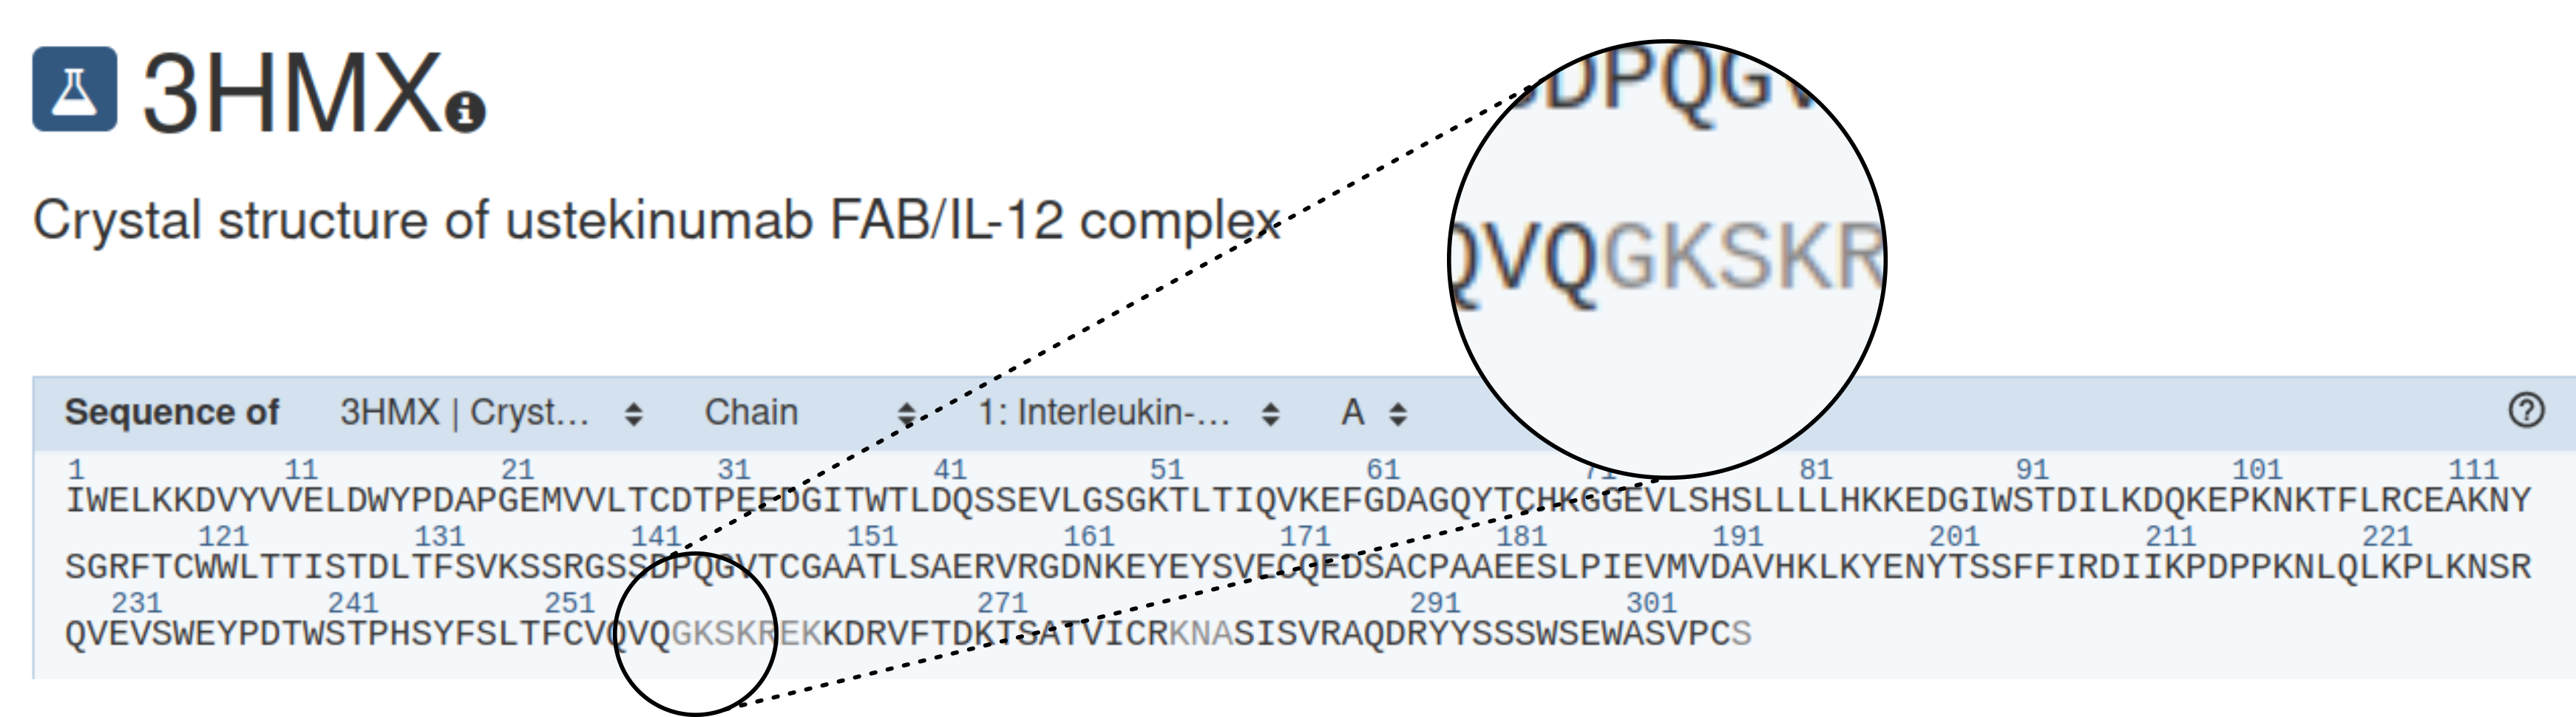
\includegraphics[width=0.45\textwidth]{figures/3hmx.png}
    \caption{Webpage of RCSB with PDB code 3HMX. The missing residues of Interleukin-12 subunit alpha are light grey instead of black.}
    \label{fig:3HMX}
\end{figure}

The structure and sequence are made available through the online repository in \code{01\_receptor\_prep/} under the names \code{3hmx.pdb} and \code{3hmx.fasta}, both of which may be inspected via a text editor. Only two segments of the molecular complex in \code{3hmx.pdb} are of interest: the Interleukin-12 subunit alpha (chain A) and Interleukin-12 subunit beta (chain B). These two chains can be written into a new file \code{hmx.pdb} using grep and regular expressions.

\begin{lstlisting}[language=bash]
grep  -E 'ATOM\s+[0-9]+\s+[A-Z]+\s+[A-Z]+\s+A' 3hmx.pdb > hmx.pdb
echo "TER" >> hmx.pdb
grep  -E 'ATOM\s+[0-9]+\s+[A-Z]+\s+[A-Z]+\s+B' 3hmx.pdb >> hmx.pdb
\end{lstlisting}

Chain A and B sequences also need to be extracted into a new file called \code{hmx.fasta}. The sequences can be copied from the aforementioned \code{3hmx.fasta}, however, the formatting needs to conform to \texttt{MODELLER} input rules. Therefore, the content of \code{hmx.fasta} should look like the following (with the complete sequences):

\begin{lstlisting}
>P1;hmx
sequence:hmx:::::::0.00:0.00
<CHAIN-A-SEQUENCE>/
<CHAIN-B-SEQUENCE>*
\end{lstlisting}
The text \code{hmx} is the align code used by \texttt{MODELLER} for the next step. The sequences of chains A and B can be found in the \code{3hmx.fasta} file downloaded from RCSB. The \code{/} symbol in the file indicates the end of a chain and the start of the next chain, and the \code{*} symbol indicates the end of all protein sequences.\\
The homology modelling software MODELLER\cite{SALI1993779} takes the sequence alignment file and the structure template to model a complete structure. Modelling the missing residues consists of two steps: sequence alignment and homology modelling.\\
Sequence alignment finds missing residue positions in the structural file and can be done using the Python script \code{salign.py} deposited in the online repository at \code{01\_receptor\_prep}. Users are encouraged to familiarise themselves with its content. This python script reads the structure from \code{hmx.pdb} with an align code \code{hmx\_structure} and aligns it with the sequence from \code{hmx.fasta} with an align code \code{hmx}. With the correct environment activated, the script can be run with the following command:
\begin{lstlisting}[language=bash]
mod10.4 salign.py # you can ignore the 'import site' failed message
\end{lstlisting}
The sequence alignment output is written to \code{hmx.ali} and consists of the original \texttt{fasta} string and the aligned string that contains gap insertion symbols \code{-}. The gap insertion symbol communicates missing residues to \code{model.py} in the next step, and therefore, any \code{-} must be aligned on a missing residue. However, the \code{-} placement can be erroneous and must be manually modified to replace the missing residues from the \texttt{hmx\_structure} sequence by the dash sign. The missing residues can be looked up at the PDB website \url{www.rcsb.org/3d-view/3HMX/1}, printed in light grey instead of black, as mentioned before. Each grey letter should be replaced with a \code{-} in \code{hmx.ali}. From experience however, \code{hmx.ali} contains a mistake at the boundary of the two sequences \code{S/RNLPVATPDPGMFP}. Technically, the gap insertion by \code{salign.py} should result in \code{-/-{}-{}-{}-{}-{}-{}-{}-{}-{}-{}-MFP}, but usually, the first dash and the \code{M} is misplaced requiring a manual fix. Thus, the correctness of \texttt{modeller} usually requires quality control.\\
With a corrected sequence alignment file \code{hmx.ali}, the program \code{model.py} can be used to construct the coordinates of the missing residues. The program generates the homology model using the \code{automodel} module with the DOPE scoring method. The Python script can be executed similarly for \code{salign.py}.
\begin{lstlisting}[language=bash]
mod10.4 model.py
\end{lstlisting}
This generates 5 models called \code{hmx.B9999000[1-5].pdb}. \texttt{MODELLER} uses a simulated annealing method to generate the structure. This method consists of minimization, heat-up, cool-down and again minimization, which can be tracked via the following commands:
\begin{lstlisting}[language=bash]
vi hmx.D00000001  # whole progress for the first model
tail -n 10 hmx.D*  # check the final energy of all models
tail -n 10 model.log  # check DOPE score of all models 
\end{lstlisting}
The energy and the DOPE score guide in selecting the most promising homology model; in some cases, the first structure is not the highest-scoring one. Herein, \code{hmx.B99990001.pdb} serves as the target structure.\\
As an intermediate test, the current directory contains a Jupyter Notebook named \code{01\_interface\_visualisation.ipynb}. The Jupyter Notebook can be opened, and all cells may be executed to visualize the structure. The notebook reads the prepared receptor file and calculates the interface residues via an intermolecular, interatomic cut-off distance of \SI{5}{\angstrom}. Upon successful execution, the visualization within the notebook should appear similar to \fref{fig:interface_residues_3hmx}. The interface allows the user to control the visualization with the mouse keys. While the left button rotates the structure, the right button translates it. Residues or atoms can be centred in the visualization by left-clicking on a particle of choice. Zooming in can be achieved by scrolling up with the mouse wheel.

\begin{figure}[H]
\centering
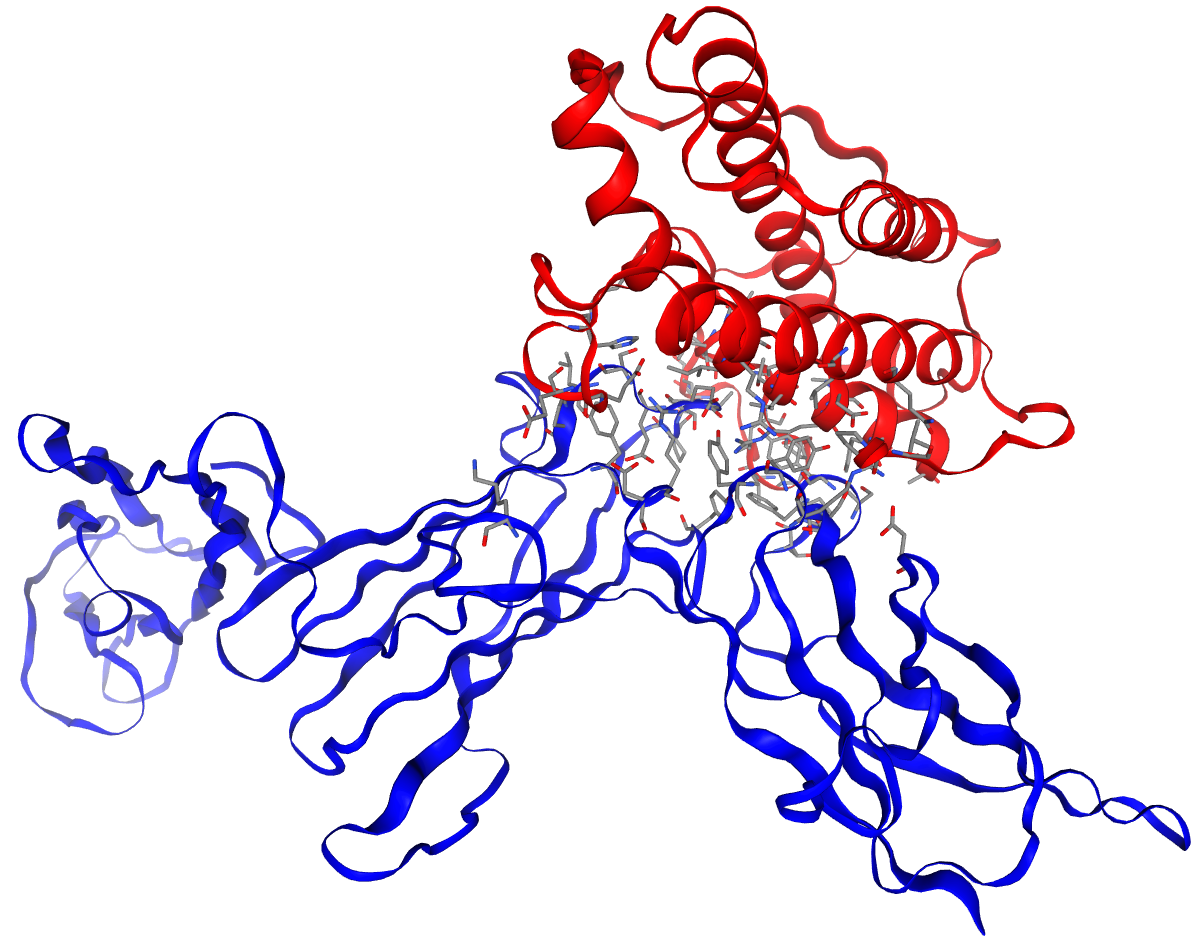
\includegraphics[width=0.45\textwidth]{figures/interface_residues_3hmx.png}
\caption{Visualization of the residue ID and the protein complex. The interface residues of protein A (blue cartoon) and protein B (red cartoon) are shown in the licorice representation.}
\label{fig:interface_residues_3hmx}
\end{figure}

Next, the \texttt{PDB} receptor file needs to be converted to \texttt{PDBQT} format in order to be compatible with \code{autodock\_gpu} and \code{vina} docking. Usage of \texttt{MGLTools} can be started as shown before by simply typing \code{pmv} in the command line.
\begin{lstlisting}[language=bash]
pmv
\end{lstlisting}
First, the receptor molecule must be loaded by clicking \code{file} $\Rightarrow$ \code{Read Molecule} at the upper left corner of the GUI. The path to the receptor molecule is \code{01\_receptor\_prep/hmx.B99990001.pdb}. In order to save the receptor in \texttt{PDBQT} format, follow the instructions shown in \fref{fig:mgltools_process_guide}. There are six steps to save the \texttt{PDBQT} file of the receptor, which entails selecting the macromolecules and saving it with the correct name, output directory and format. 

\begin{figure}[H]
\centering
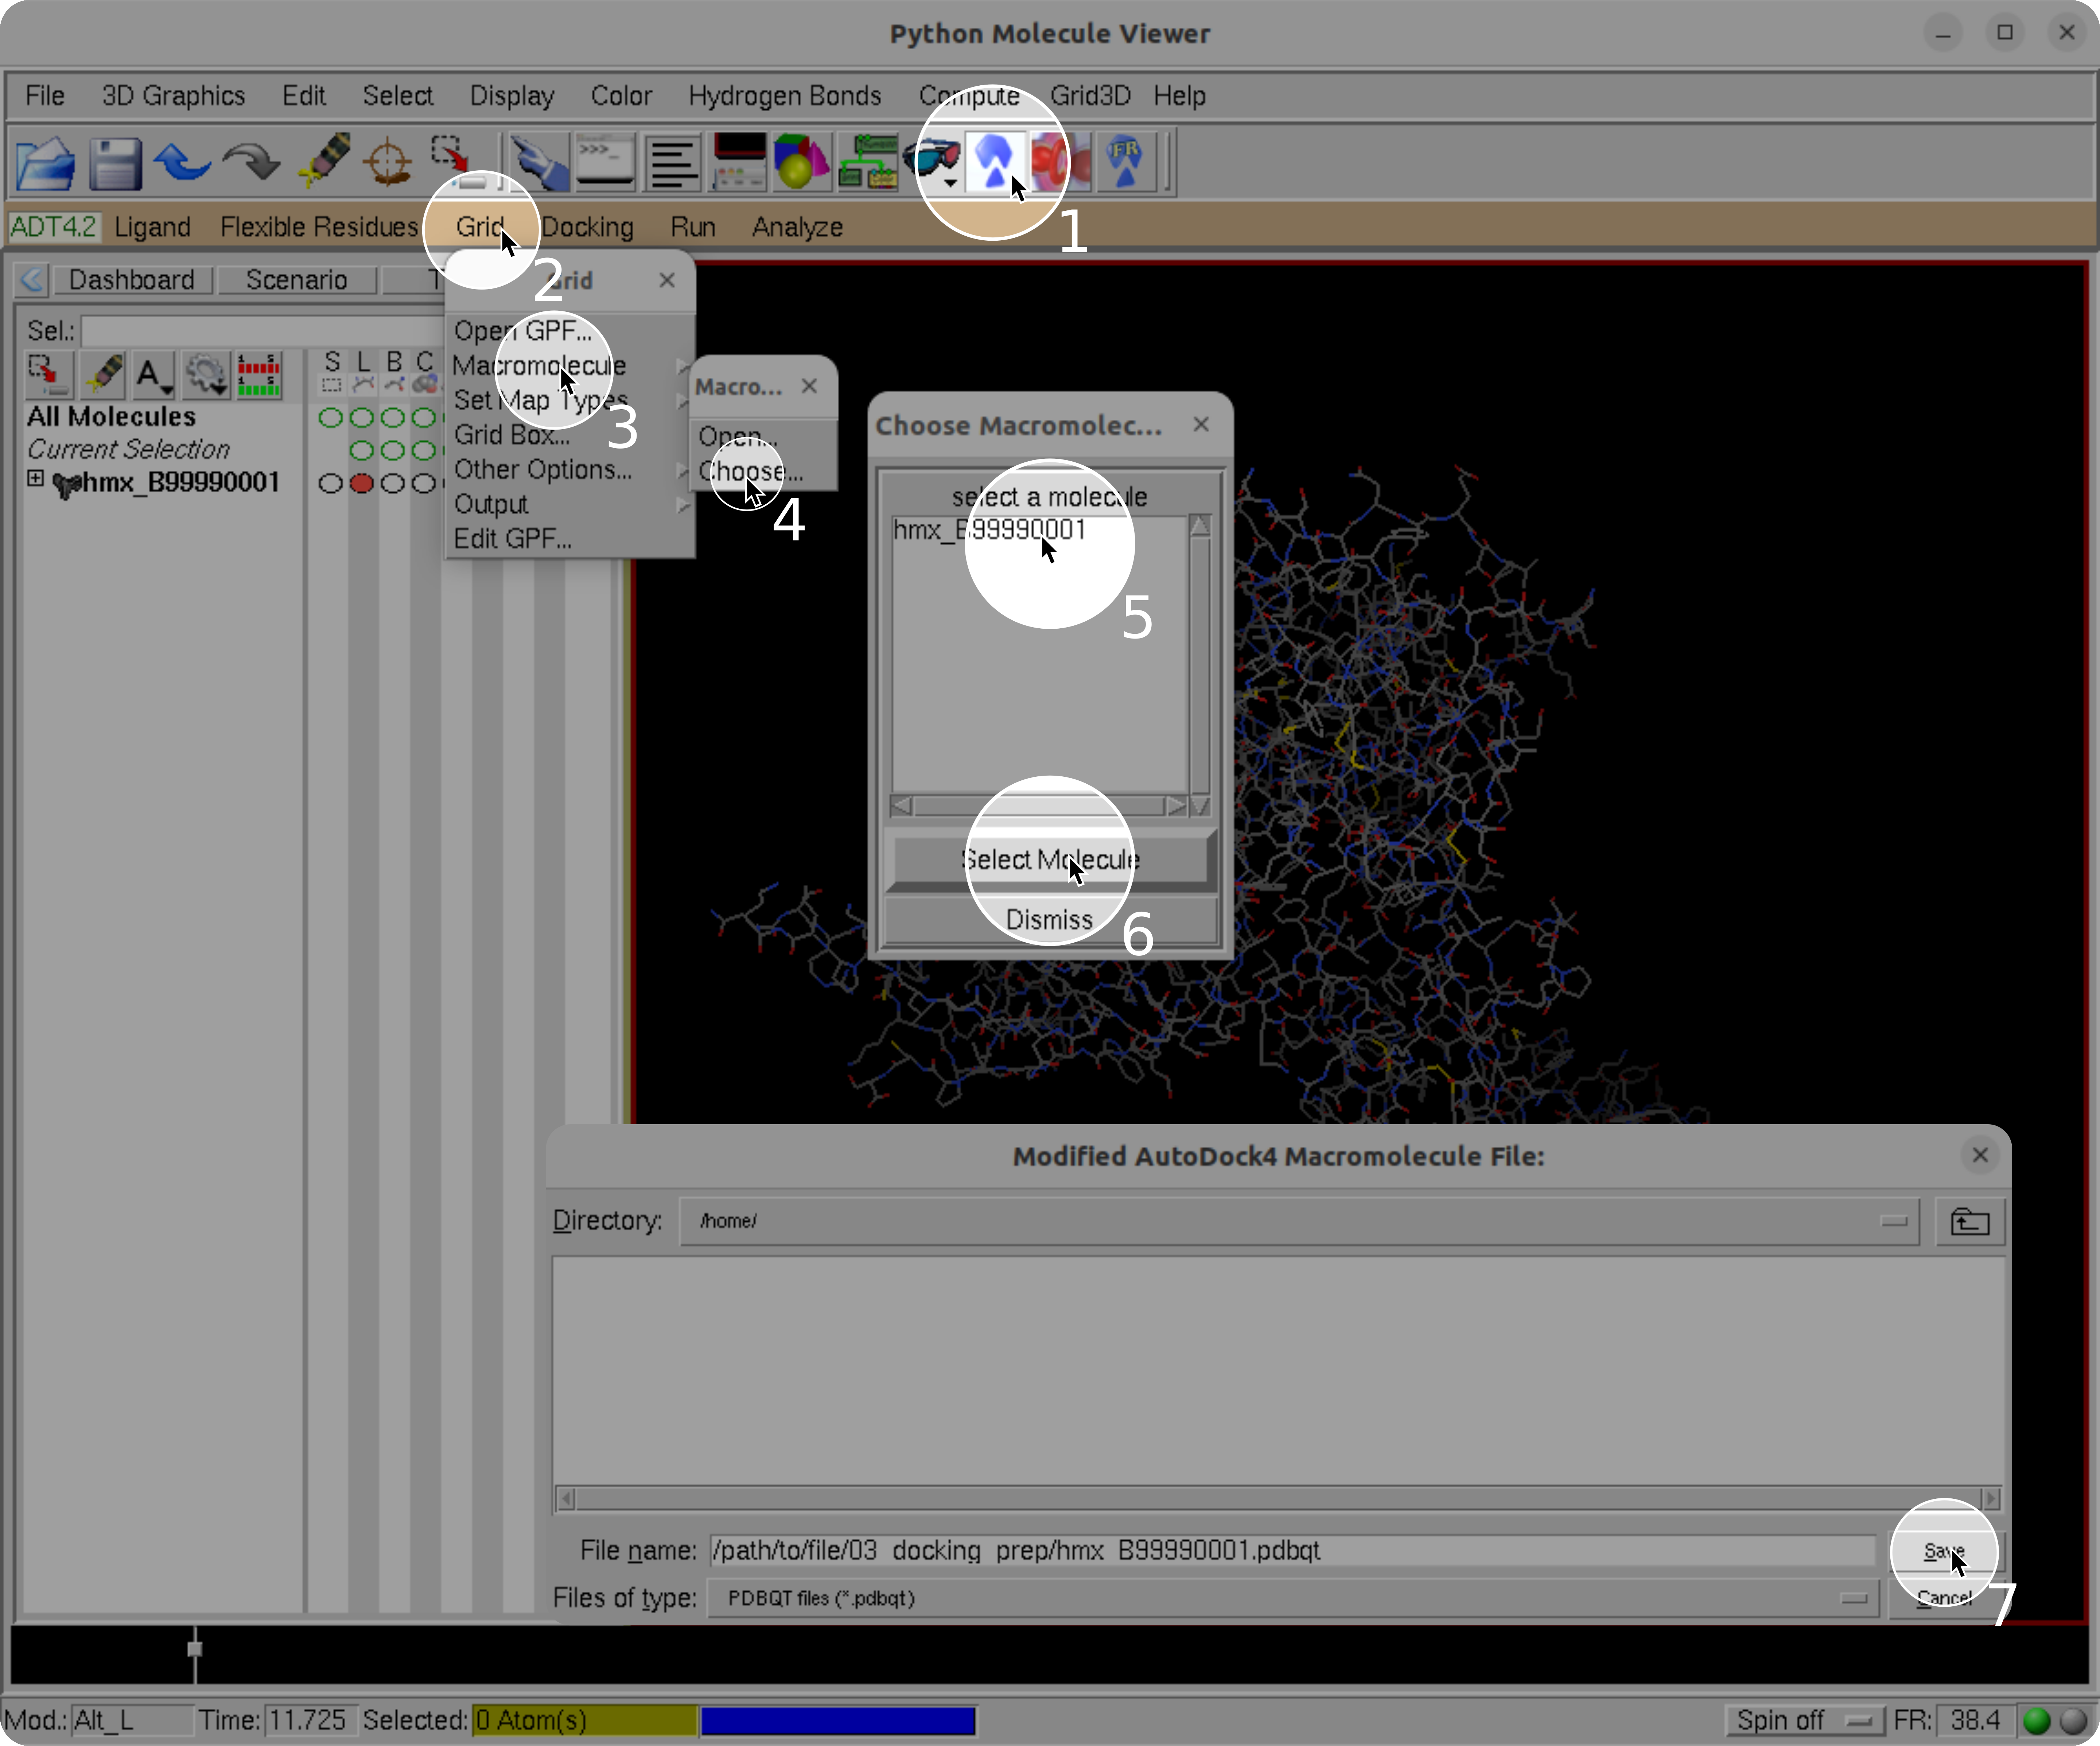
\includegraphics[width=0.45\textwidth]{figures/mgltools_process_guide.png}
\caption{Generating \texttt{PDBQT} for the receptor using \texttt{MGLTools}. First, click the AutoDock-icon, then click on the newly opened \code{Grid} button and select \code{Macromolecule} and \code{Chose...}. After that, a new window should open with only one molecule to select, which should then be saved as \code{03\_docking\_prep/hmx.B99990001.pdbqt}.}
\label{fig:mgltools_process_guide}
\end{figure}


\subsection*{Interface Pocket Detection}
With a complete receptor available, the next step is to make out the receptor pocket for compound docking. A good PPI stabilizer needs to bind evenly to both interfaces of the complex macromolecules. A compound that binds strongly to one protein but weakly to the other acts as a competitive inhibitor, adverse to the intended behaviour. To detect a druggable pocket at the complex interface, \texttt{Fpocket}\cite{le_guilloux_fpocket_2009} can be used.\\
The algorithm behind \texttt{Fpocket} identifies pockets via a geometrical criterion. The program is quite sophisticated, but in all brevity, numerous so-called alpha spheres are fitted onto the protein surface and expanded until four points of the protein surface contact the respective sphere. Spheres with a large radius must be located at the flat surface and are discarded, while spheres within a crevice of the protein remain small and indicate pockets. This is followed by clustering the spheres into individual pockets and ranking the spheres based on descriptor-based pocket scoring and drug-scoring methods.\cite{le_guilloux_fpocket_2009} After activating the micromamba environment, the program can be executed straightforwardly.
\begin{lstlisting}[language=bash]
fpocket -f hmx.B99990001.pdb
\end{lstlisting}
Once successfully executed, \code{fpocket} generates a folder \code{hmx.B99990001\_out/}. After changing into this directory, the pockets can be visualized by executing a custom bash script.
\begin{lstlisting}[language=bash]
cd hmx.B99990001_out/
bash hmx.B99990001_PYMOL.sh
\end{lstlisting}
Executing said bash script should open a \texttt{PyMOL} window with the two protein chains and the pockets that were found by \texttt{Fpocket} (similar to \fref{fig:fpocket_allpockets}). Further information about all detected pockets can be found in the \code{hmx.B99990001\_out/pockets/} folder. The residues that form the pocket are written to \code{pocket*\_atm.pdb}, and the position of the probes are written in \code{pocket*\_vert.pqr}. Several pocket properties of the first pocket can be inspected using the following line of code:
\begin{lstlisting}[language=bash]
head hmx.B99990001_out/pockets/pocket1_atm.pdb -n 20
\end{lstlisting}
\begin{figure}[H]
    \centering
    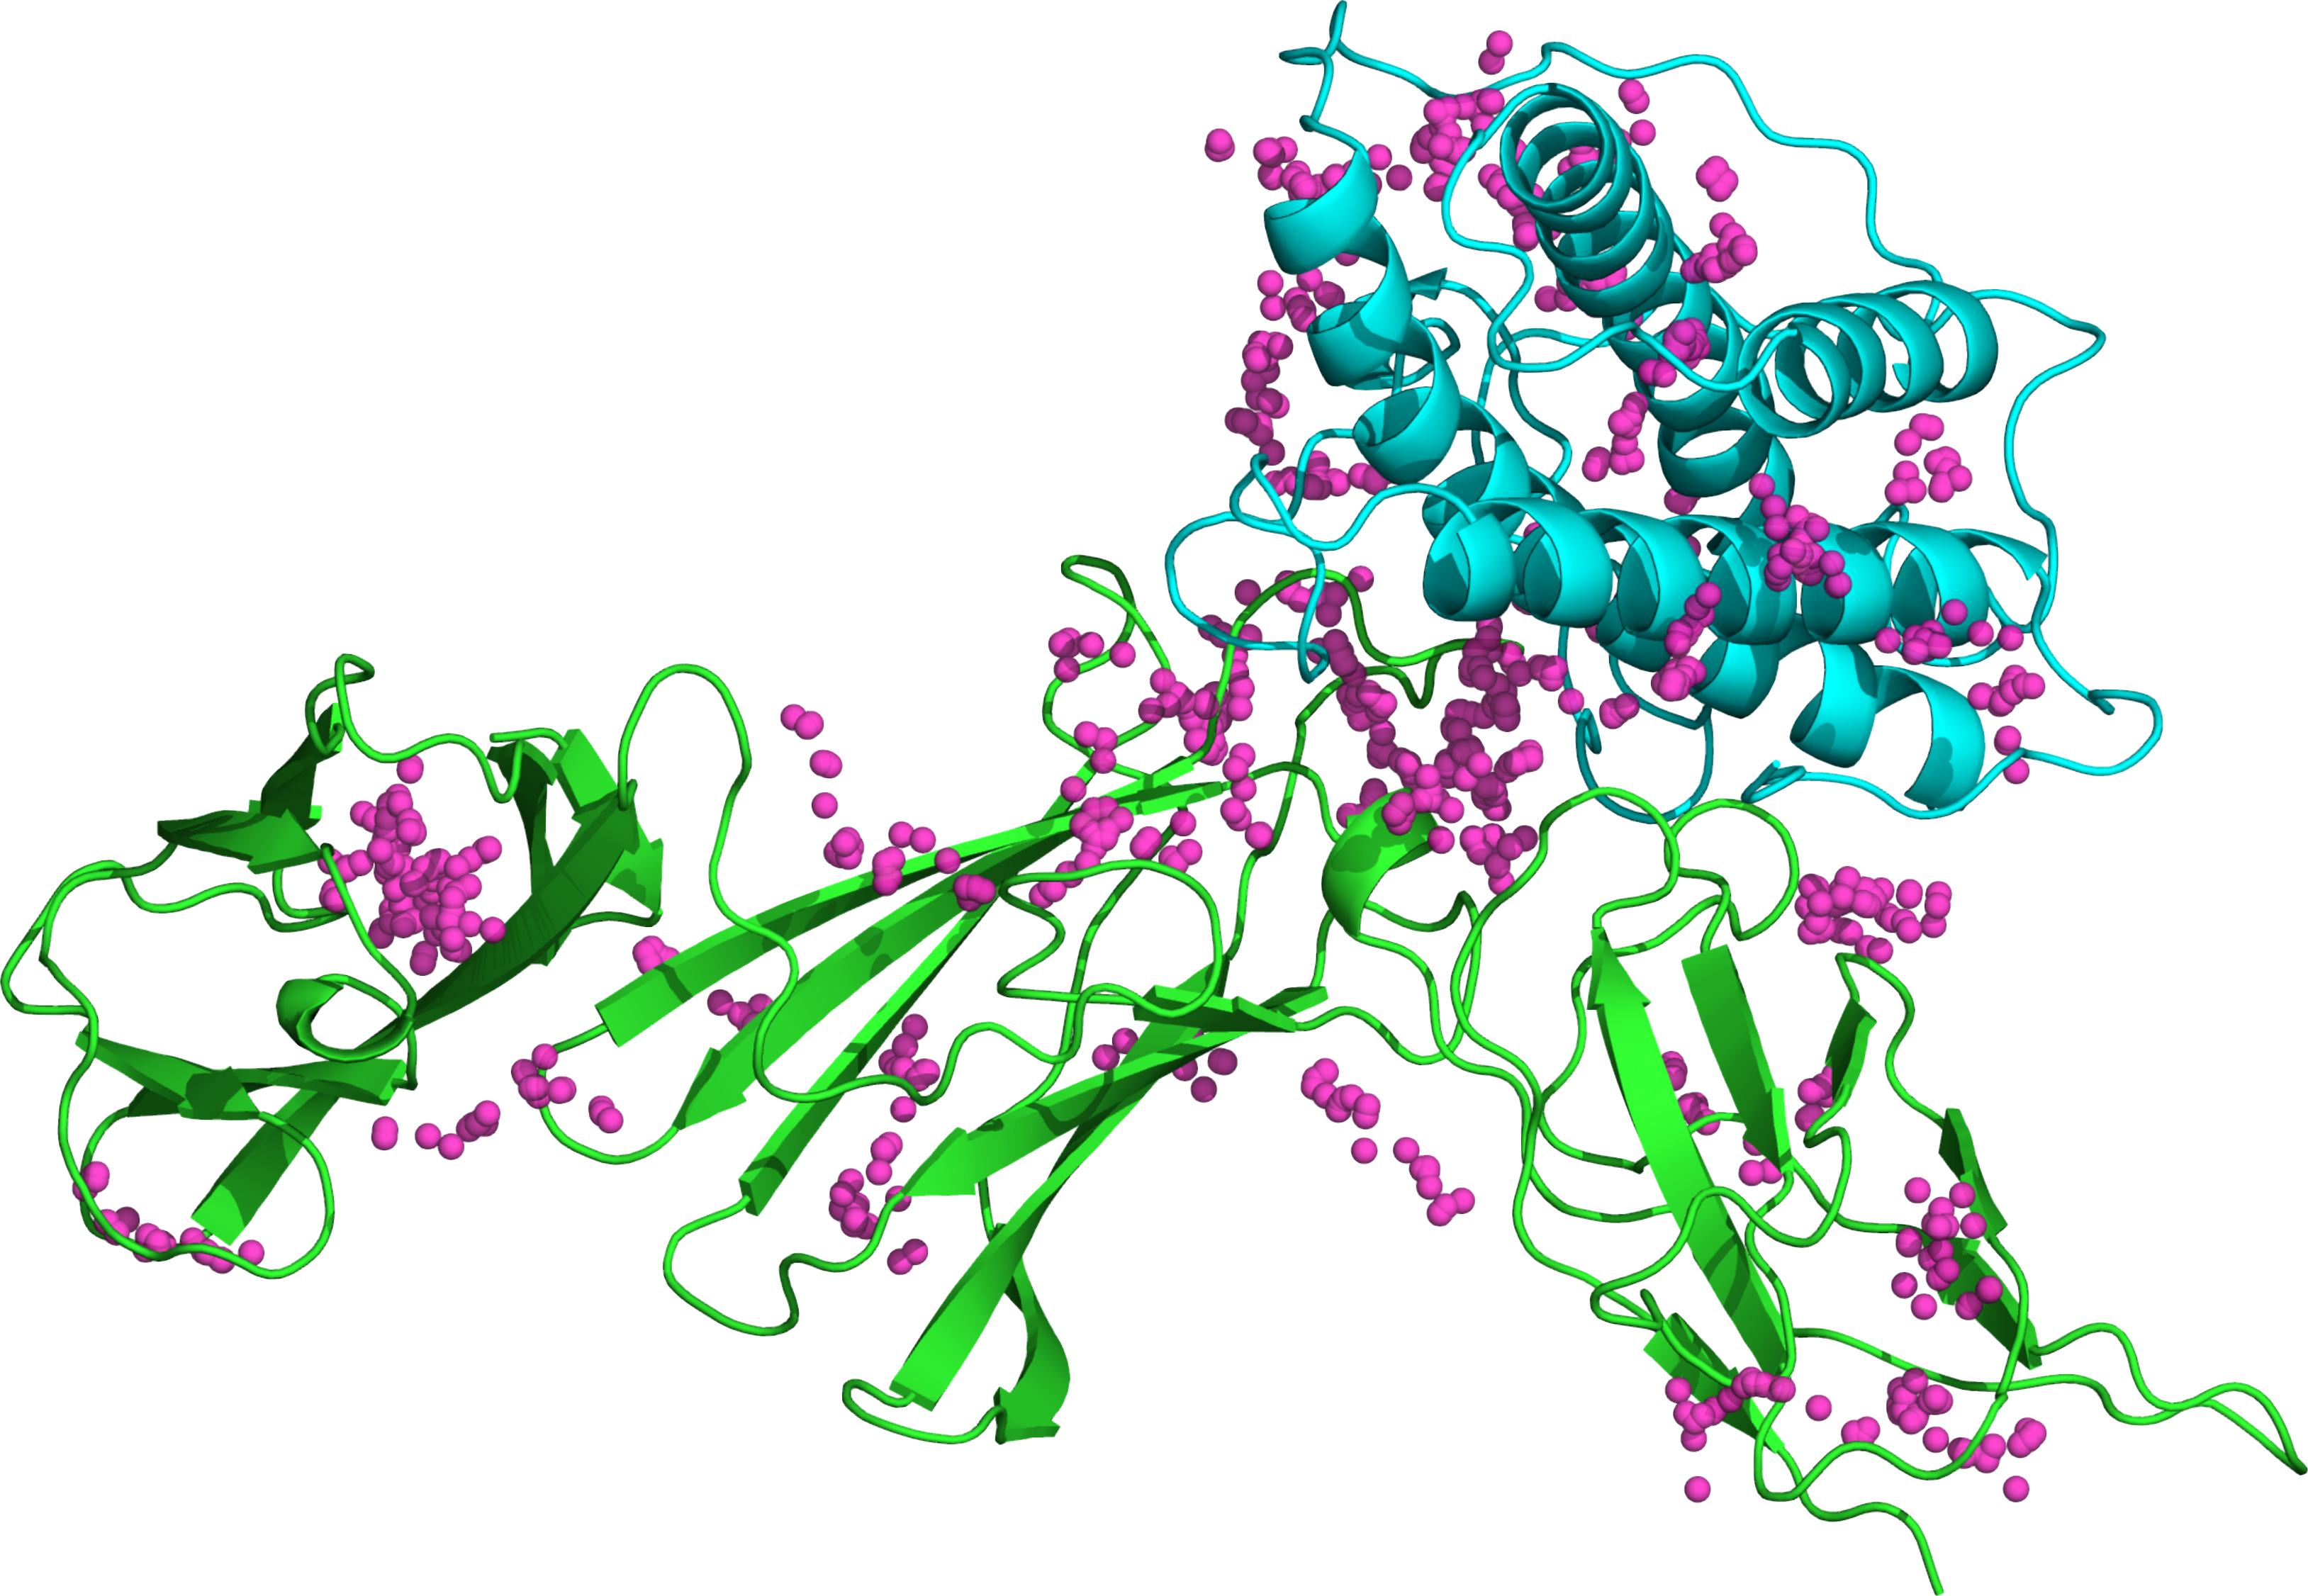
\includegraphics[width=0.45\textwidth]{figures/fpocket_allpockets.png}
    \caption[All pockets found by \code{fpocket} and visualised via \code{pymol}]{All pockets found by \code{fpocket} and visualised via \code{pymol}. One chain is shown in green, the other one is shown in cyan, and the pockets are shown in magenta.}
    \label{fig:fpocket_allpockets}
\end{figure}
Nevertheless, information about a possible protein-protein interface is not present, and therefore, a pocket that forms contacts with both proteins must be identified differently. Furthermore, the viability of each interfacial pocket might vary, and unusable pockets need to be excluded from further analysis. Therefore, another Jupyter Notebook called \code{02\_pocket\_analysis.ipynb} can be found in \code{01\_receptor\_prep} which handles the pocket assessment. When executing, the cells should calculate the solvent-accessible surface area (SASA) and buried surface area (BSA) of the two proteins and each pocket, respectively. Here, all pocket probes resemble artificial ligands. The BSA of pocket $P$ within protein A is obtained by summing up the SASA of protein A and the pocket ($SASA_\text{\tiny A}$, $SASA_\text{\tiny P}$) and then subtracting the $SASA_\text{\tiny AP}$ of the complex of the two.
\begin{equation}
    BSA_\text{\tiny PA} = (SASA_\text{\tiny A} + SASA_\text{\tiny P}) - SASA_\text{\tiny AP} 
\end{equation}
The BSA of protein B and the pocket is evaluated analogously in the Jupyter Notebook. A criterion for a good stabilizer binding pocket is a large BSA with both proteins and a good pocket score and drug score. If all cells in the Jupyter Notebook are executed successfully, plots should appear similar to \fref{fig:BSA_drugscore}. In this example, the best pockets can be identified as pocket 1 and 4 since both have a high $BSA_\text{\tiny min}$ and a high drug score. 

\begin{figure}[H]
\centering
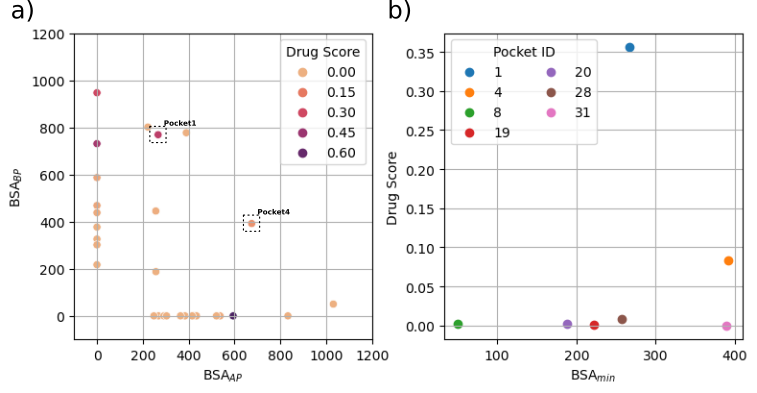
\includegraphics[width=0.45\textwidth]{figures/BSA_drugscore.png}
\caption{Data visualization of the protein-pocket BSA and drug score. \textbf{a)} Distribution of $BSA_\text{\tiny AP}$ and $BSA_\text{\tiny BP}$ of all detected pockets with color coded drug score. \textbf{b)} Distribution of $BSA_\text{\tiny min}$ and Drug score of the interface pockets.}
\label{fig:BSA_drugscore}
\end{figure}

A closer look into \fref{fig:BSA_drugscore} reveals that the BSA values for pocket 4 are more balanced, making it the most favourable pocket. Should two pockets' BSAs score equally well, the drug score is also reported by \code{fpocket} and can be used to settle ties. The primary output of \code{02\_pocket\_analysis.ipynb} is a file called \code{config}, which maps out the best available pocket (according to the user's assessment) in a format compatible with \code{autodock\_gpu} and \code{vina}. It is recommended to generate one \code{config} only since the filename \code{config} is hard coded in \code{03\_docking\_prep/vina.sh}, a later step. Any user aiming to analyze two or more pockets must be prepared to manually alter downstream executables. Contentwise, \code{config} contains the information about the box centre and box dimensions in absolute coordinates; thus, changing the coordinates of the receptor \texttt{PDB} file would invalidate the \code{config} file. The Jupyter Notebook also contains cells to visually inspect eventual candidates. The cell output should look somewhat similar to \fref{fig:pocket_visualization_3hmx}. 

\begin{figure}[H]
\centering
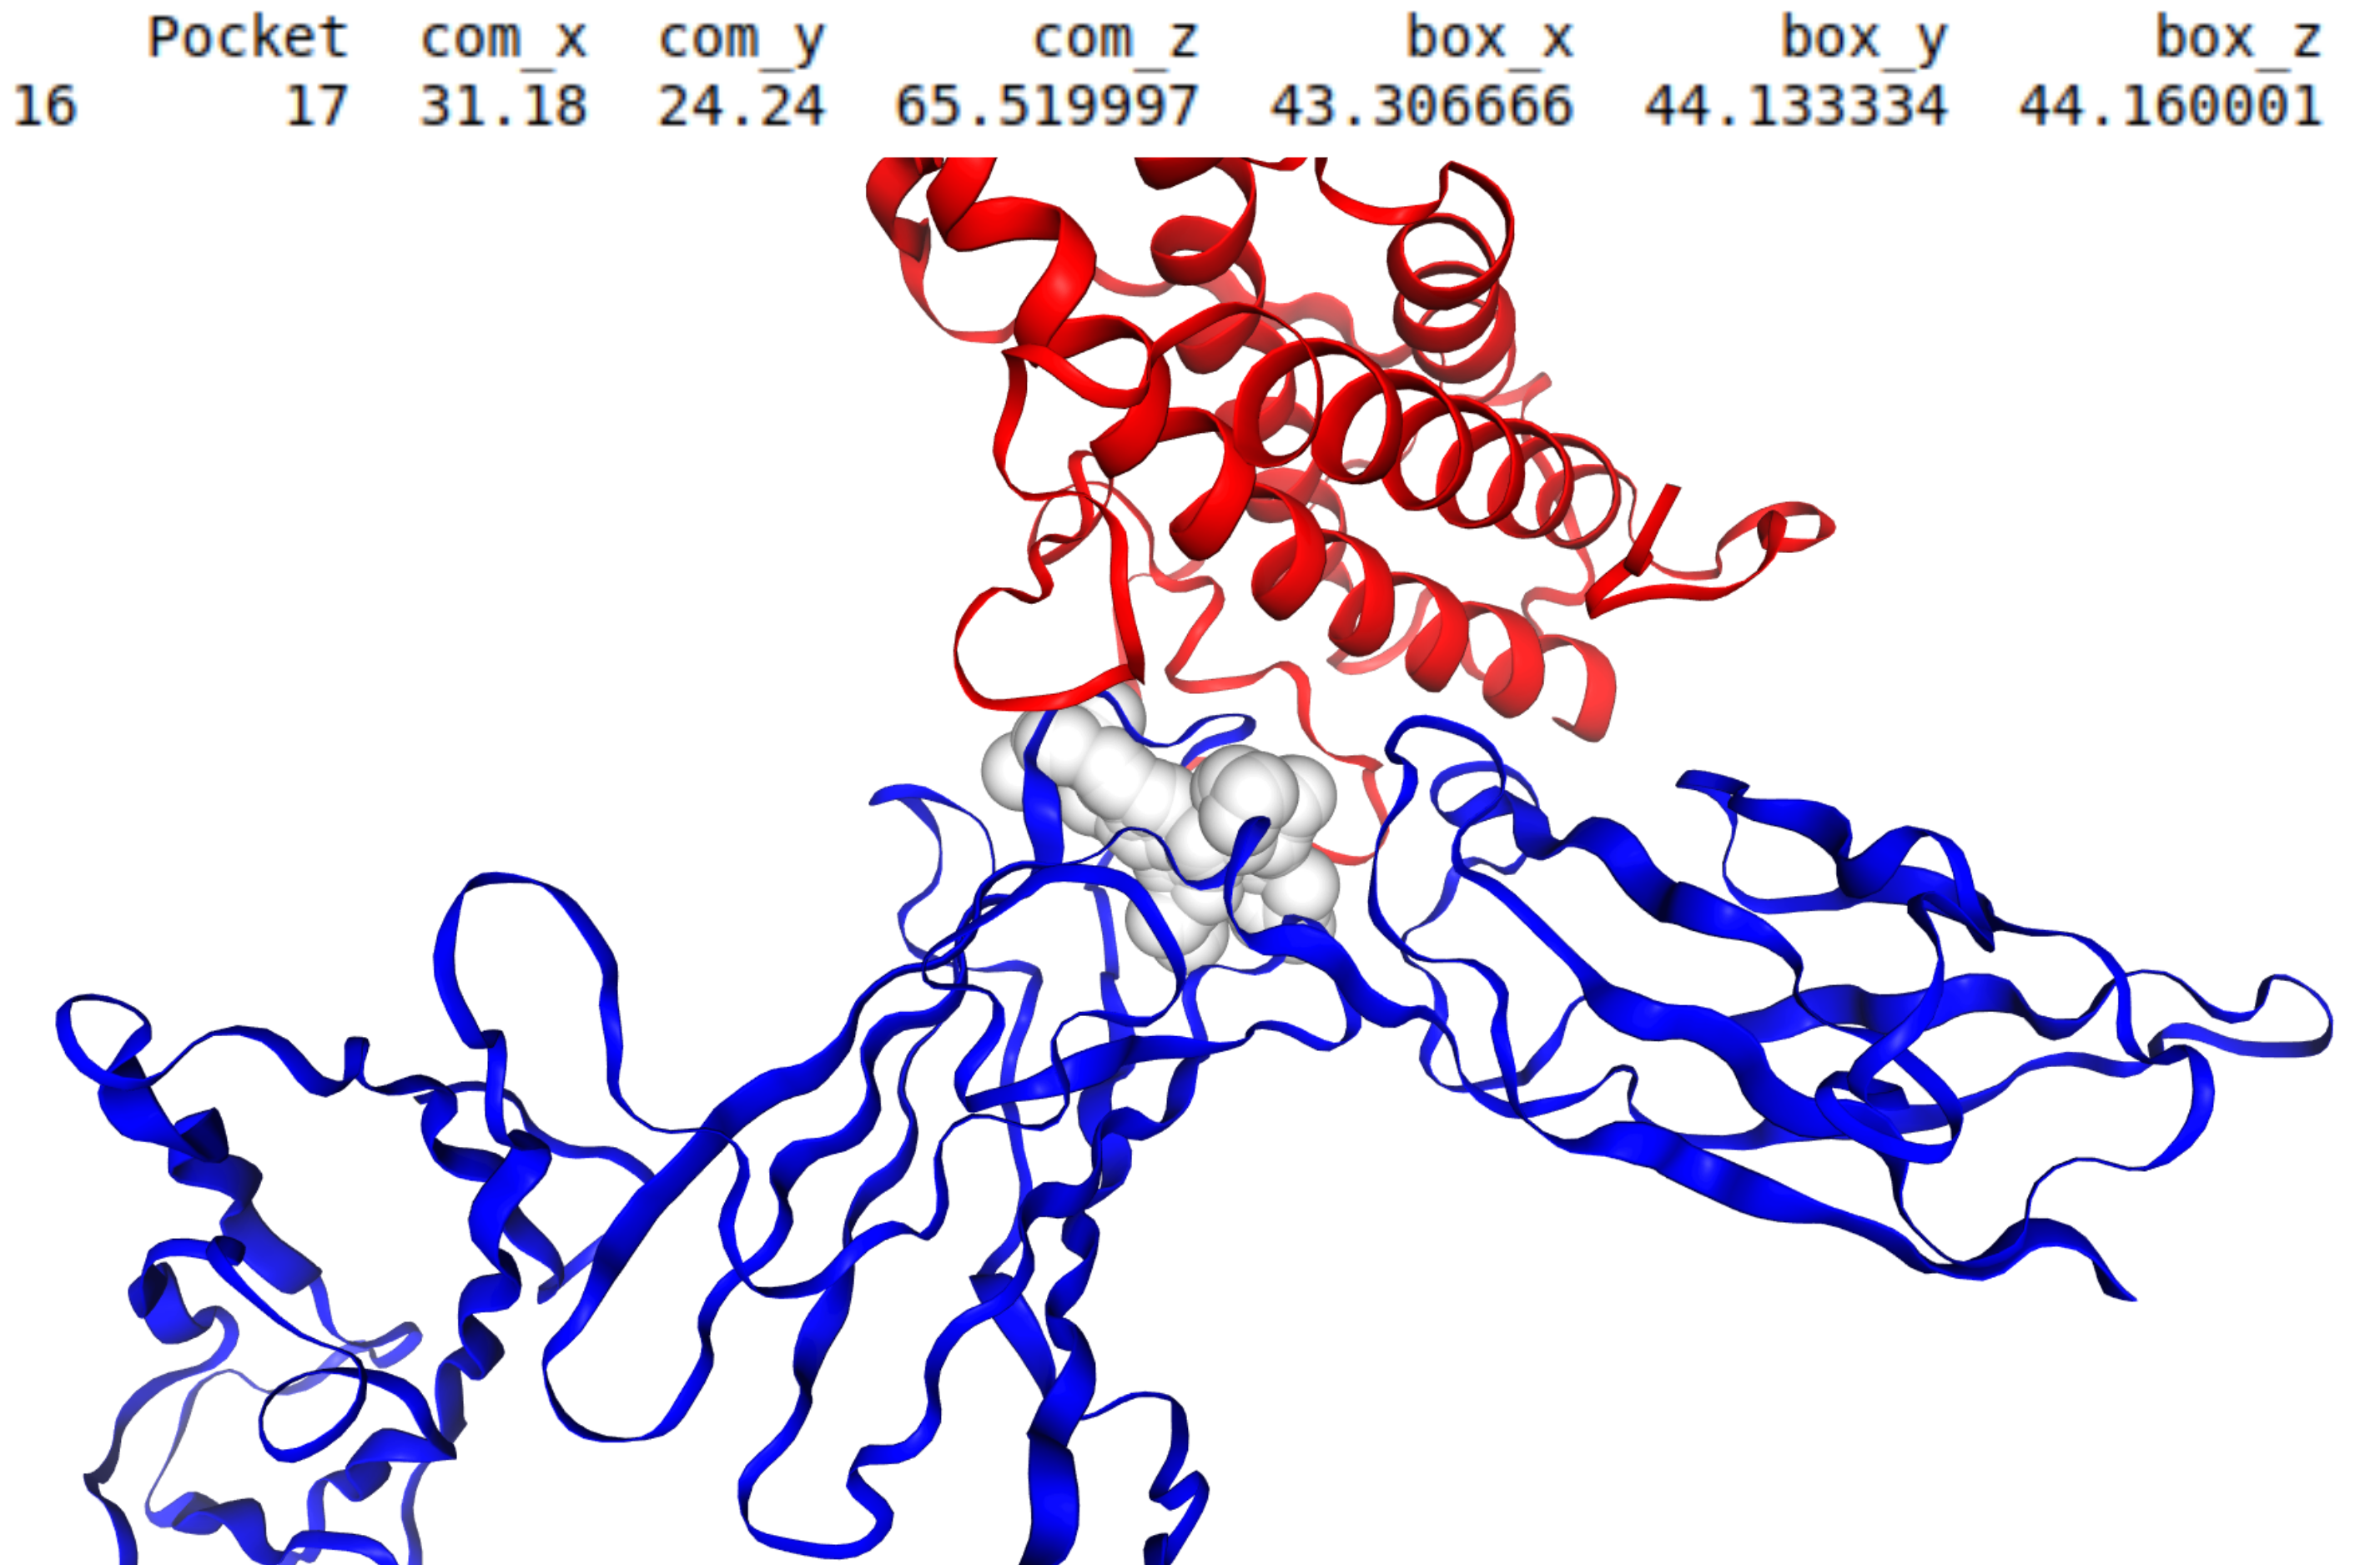
\includegraphics[width=0.45\textwidth]{figures/visualize_pocket_3hmx.png}
\caption{Structure visualization with a detected pocket. The center of mass (COM) and box size information are also printed on the top of the graphic.}
\label{fig:pocket_visualization_3hmx}
\end{figure}

With the pocket selected, it is good practice to visualize the binding pocket to check if it matches the findings in \code{01\_receptor\_prep/}. The GUI of \texttt{MGLtools} can be used for that purpose. As stated above, it can be opened via \code{pmv}. After reading-in the \texttt{PDBQT} receptor file, 
the \texttt{Grid Box} button can be used to visualize the volume to be used for molecular docking (see \fref{fig:mgltools_process_guide}). By clicking this button, a panel of box size parameters will open. The parameters should be adjusted according to \code{config} in the current directory to see if the box matches the preferable binding pocket picked by the user. The contents of the \code{config} file should look similar to the example file printed below.
\begin{lstlisting}[language=bash]
center_x =  27.83  # box' x-center in Angstrom
center_y =  38.78  # box' y-center in Angstrom
center_z =  56.71  # box' z-center in Angstrom
size_x = 40   # box' x-size in vina npts
size_y = 32   # box' y-size in vina npts
size_z = 40   # box' z-size in vina npts
\end{lstlisting}
For better visualization, the ribbon representation of the protein can be activated by clicking the circle under the \code{R} column on the left panel shown in \fref{fig:mgltools_process_guide}. At the same time, deactivating the circle under the \code{L} column removes the atomic licorice representation. Additionally, each complex molecule can be coloured individually by clicking the triangle below the \code{Cl} column and choosing the colouring scheme \code{By Chain}. The emerging structure should look similar to \fref{fig:pocket_visualization_3hmx}, particularly concerning pocket position and dimension.


\subsection*{Ligand Preparation}
With a fully prepared receptor pocket, the next step is to prepare the ligands for docking. In theory, there are around $10^{60}$ \textit{drug-like} compounds\cite{Reymond_2015}, which are impossible to screen through with current computer hardware. Instead, we want to use the ZINC20 database in this demonstration. Although the ZINC20 database contains fewer compounds than $10^{60}$, it is still not feasible to screen it whole. Therefore, some filters will be applied to further reduce the amount of compounds for docking.

Two stages of filtering are applied in this exercise. The first one is integrated into the query system of the ZINC database itself. The second filtering stage is a custom program that can be adapted to fit numerous scientific criteria and utilizes the Python package \code{rdkit}\cite{rdkit}. The ZINC database can be queried directly on the webpage (\url{zinc20.docking.org/}). The online filtering process is laid out in \fref{fig:zincligands_download_guide} and comprises $\log P$ and molecular weight filtering, which translates to hydrophobicity and size of the compounds. The process of downloading a fraction of the database's compounds is illustrated in the exact figure. This fraction still entails around 4 million compounds.

\begin{figure}[H]
\centering
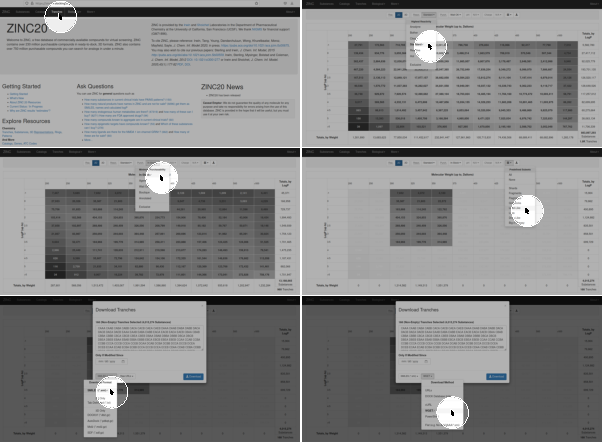
\includegraphics[width=0.45\textwidth]{figures/zincligands_download_guide.pdf}
\caption{In these six pictures, the workflow to narrow down compounds from the ZINC20 database is shown. First, click the \texttt{Tranches} button to access the website. Then, the large number of compounds will be filtered with custom selections, as shown in the second, third, and fourth pictures. Finally, the compounds must be downloaded as a \texttt{wget} file in SMILES format. Pictures as of June 2023.}
\label{fig:zincligands_download_guide}
\end{figure}

The compounds are downloaded in the SMILES string format, which is generally computer readable and can be processed with various programs, e.g. \texttt{RDKit} and \texttt{Open Babel}. The way SMILES are generated and work can be read into elsewhere (e.g. \url{medium.com/@luis-vollmers/tutorial-to-smiles-and-canonical-smiles-explained-with-examples-fbc8a46ca29f}). The file that was downloaded in the \texttt{wget} format is not a data file per se but an executable which will then download the respective files for the user. After moving this file from the \texttt{Downloads} directory to \code{02\_ligand\_prep}, which should be the current directory, it can be executed via \code{bash}.
\begin{lstlisting}[language=bash]
mv ~/Downloads/ZINC-downloader-2D-smi.wget ./
bash ZINC-downloader-2D-smi.wget
\end{lstlisting}
This command should start downloading several different files containing the compounds priorly filtered from ZINC20. For consistency, a new directory should be created in \code{02\_ligand\_prep} called \code{SMILES/}. With the following commands, the \texttt{SMI} files can be transferred into \code{SMILES/}, and the empty directories are removed.
\begin{lstlisting}[language=bash]
mkdir -p SMILES/
mv -v */*.smi SMILES/
rmdir ./*
\end{lstlisting}
After moving all \texttt{SMI} files into the SMILES directory, the index row can be deleted via \code{sed}.
\begin{lstlisting}[language=bash]
for i in SMILES/*.smi; do sed -i '/smiles/d' $i;  done
\end{lstlisting}
The last steps in compound filtering include the execution of the Python script \code{filter\_smiles.py}, as well as concatenating all filtered compounds into one file. The latter should not precede the former since executing the Python script on a large SMILES list can lead to memory overflow. The Python program reads in a text file containing SMILES strings in each row and applies certain filter criteria to the compounds. The criteria chosen in \code{filter\_smiles.py} are arbitrary, and their only purpose is to show how to filter compounds in a database given prior pharmaceutical knowledge and decrease the search space. Herein, the filters encompass a limit of four hydrogen bond donors and acceptors, the presence of one carboxy group and one benzene or imidazole group. Furthermore, the last filter criterion is a Bertz complexity below 500. The Bertz complexity index measures the complexity of the molecular graph. These filters are implemented in \texttt{RDKit}, and users may alter them in any way. The Python program can be executed by simply calling \code{python} on \code{filter\_smiles.py} repeatedly on each file. It should run quickly and yield one filtered file in \code{SMILES/} for each unfiltered file. The following command uses a for loop to iterate through all files in \code{SMILES/}, prints the filename and executes the Python script with the output name adjusted automatically. The concatenation of filtered compounds can be achieved via the \code{cat} command, which is short for concatenate.
\begin{lstlisting}
for i in SMILES/*.smi; do echo $i; python filter_smiles.py $i ${i/.smi/_filtered.txt}; done
cat SMILES/*_filtered.txt > filtered.txt
\end{lstlisting}
The successful filtering can be assessed by printing out the line number of the output file, which should contain fewer lines than originally downloaded compounds. In this exercise, the number of downloaded compounds was around 4 million; the number of filtered compounds should be roughly 14000. The command that can be used to do so is called \code{wc}, which is short for word count. However, it counts lines given the \code{-l} flag.
\begin{lstlisting}[language=bash]
wc -l filtered.txt
\end{lstlisting}

After filtering the compounds, the next step is generating three-dimensional molecular structures, called conformers. For this task, \texttt{Open Babel} is required. The following line of code should write the desired compounds to \code{filtered.pdbqt}. Converting 14000 compounds can take quite a lot of time, so a subset should be considered. E.g. the command can be interrupted after converting around 2000 compounds by pressing \keystroke{Ctrl} + \keystroke{C} on the keyboard.
\begin{lstlisting}[language=bash]
obabel -ismi filtered.txt -opdbqt -O filtered.pdbqt --gen3d --minimize --steps 1500 --sd --ff MMFF94
\end{lstlisting}
Sometimes \code{obabel} will fail to generate a 3D structure from SMILES, which results in an error that can be ignored. There will be more than enough compounds, which will result in a successful conversion. The \texttt{PDBQT} batch files require splitting into individual ligand files so that they can be docked individually later on. Hence, a folder needs to be created in \code{02\_ligand\_prep/} called \code{PDBQT} followed by execution of \code{vina\_split} with the options shown below.
\begin{lstlisting}[language=bash]
mkdir -p PDBQT
cd PDBQT
vina_split --input ../filtered.pdbqt --ligand ligand_
\end{lstlisting}
The resulting directory contains one \texttt{PDBQT} file for each ligand with a numeric ID, e.g. \code{ligand\_0354.pdbqt}. These \texttt{PDBQT} files are the foundation for the virtual screening later in this exercise.


\subsection*{Molecular Docking}
\subsubsection*{Docking Test with AutoDock Vina}
With all three parts required for molecular docking prepared, i.e. the receptor, a receptor pocket and the ligands, the docking procedure can be tackled. Apart from the docking procedure, the surrounding computational tools are also explored. Firstly, a test should be performed to check whether everything is correctly set up before screening a large set of compounds with GPU-accelerated docking. For this test, a bash script called \code{vina.sh} is already placed in \code{03\_docking\_prep} for automatic docking of the test ligands. This bash script should be executed and will dock the ligands in the binding pocket specified in \code{config}. The ligands are read from \code{../02\_ligand\_prep/TEST/}, and the outputs are saved to \code{PDBQT/} and \code{PDB/}. The command for executing the bash script and the expected output are shown below.
\begin{lstlisting}[language=bash]
./vina.sh  # chmod 777 vina.sh might be necessary
\end{lstlisting}
\begin{lstlisting}
#################################################################
# If you used AutoDock Vina in your work, please cite:          #
[...]
[...]
[...]
Performing search ...
0%   10   20   30   40   50   60   70   80   90   100%
|----|----|----|----|----|----|----|----|----|----|
***************************************************
done.
Refining results ... done.
[...]
[...]
[...]
9 files output. The first is ./PDB/out_1.pdb
\end{lstlisting}
Apart from the \texttt{STDOUT}, this command also generates docked coordinates of the ligand molecules. \texttt{PyMOL} can visualise all docking results at once.
\begin{lstlisting}[language=bash]
pymol ../01*/hmx.B99990001.pdb ./PDBQT/*
\end{lstlisting}

The representation might be improved by showing the protein in the cartoon representation and the ligands in the licorice representation and distinguishing them via colour. On the top right panel, this can be achieved by clicking the \code{H} icon in the \code{hmx\_B9990001} row and then selecting \code{everything}. Next, clicking the \code{S} icon in the same row should be followed followed by clicking \code{cartoon}. Finally, the colouring method should be changed by clicking the (\code{C}) icon in the \code{all} row and \code{by chain} $\xrightarrow{}$ \code{by chain (elem C)} should be chosen. The resulting graphic should be somewhat similar to \fref{fig:visualize_docking_pymol}. 

\begin{figure}[H]
\centering
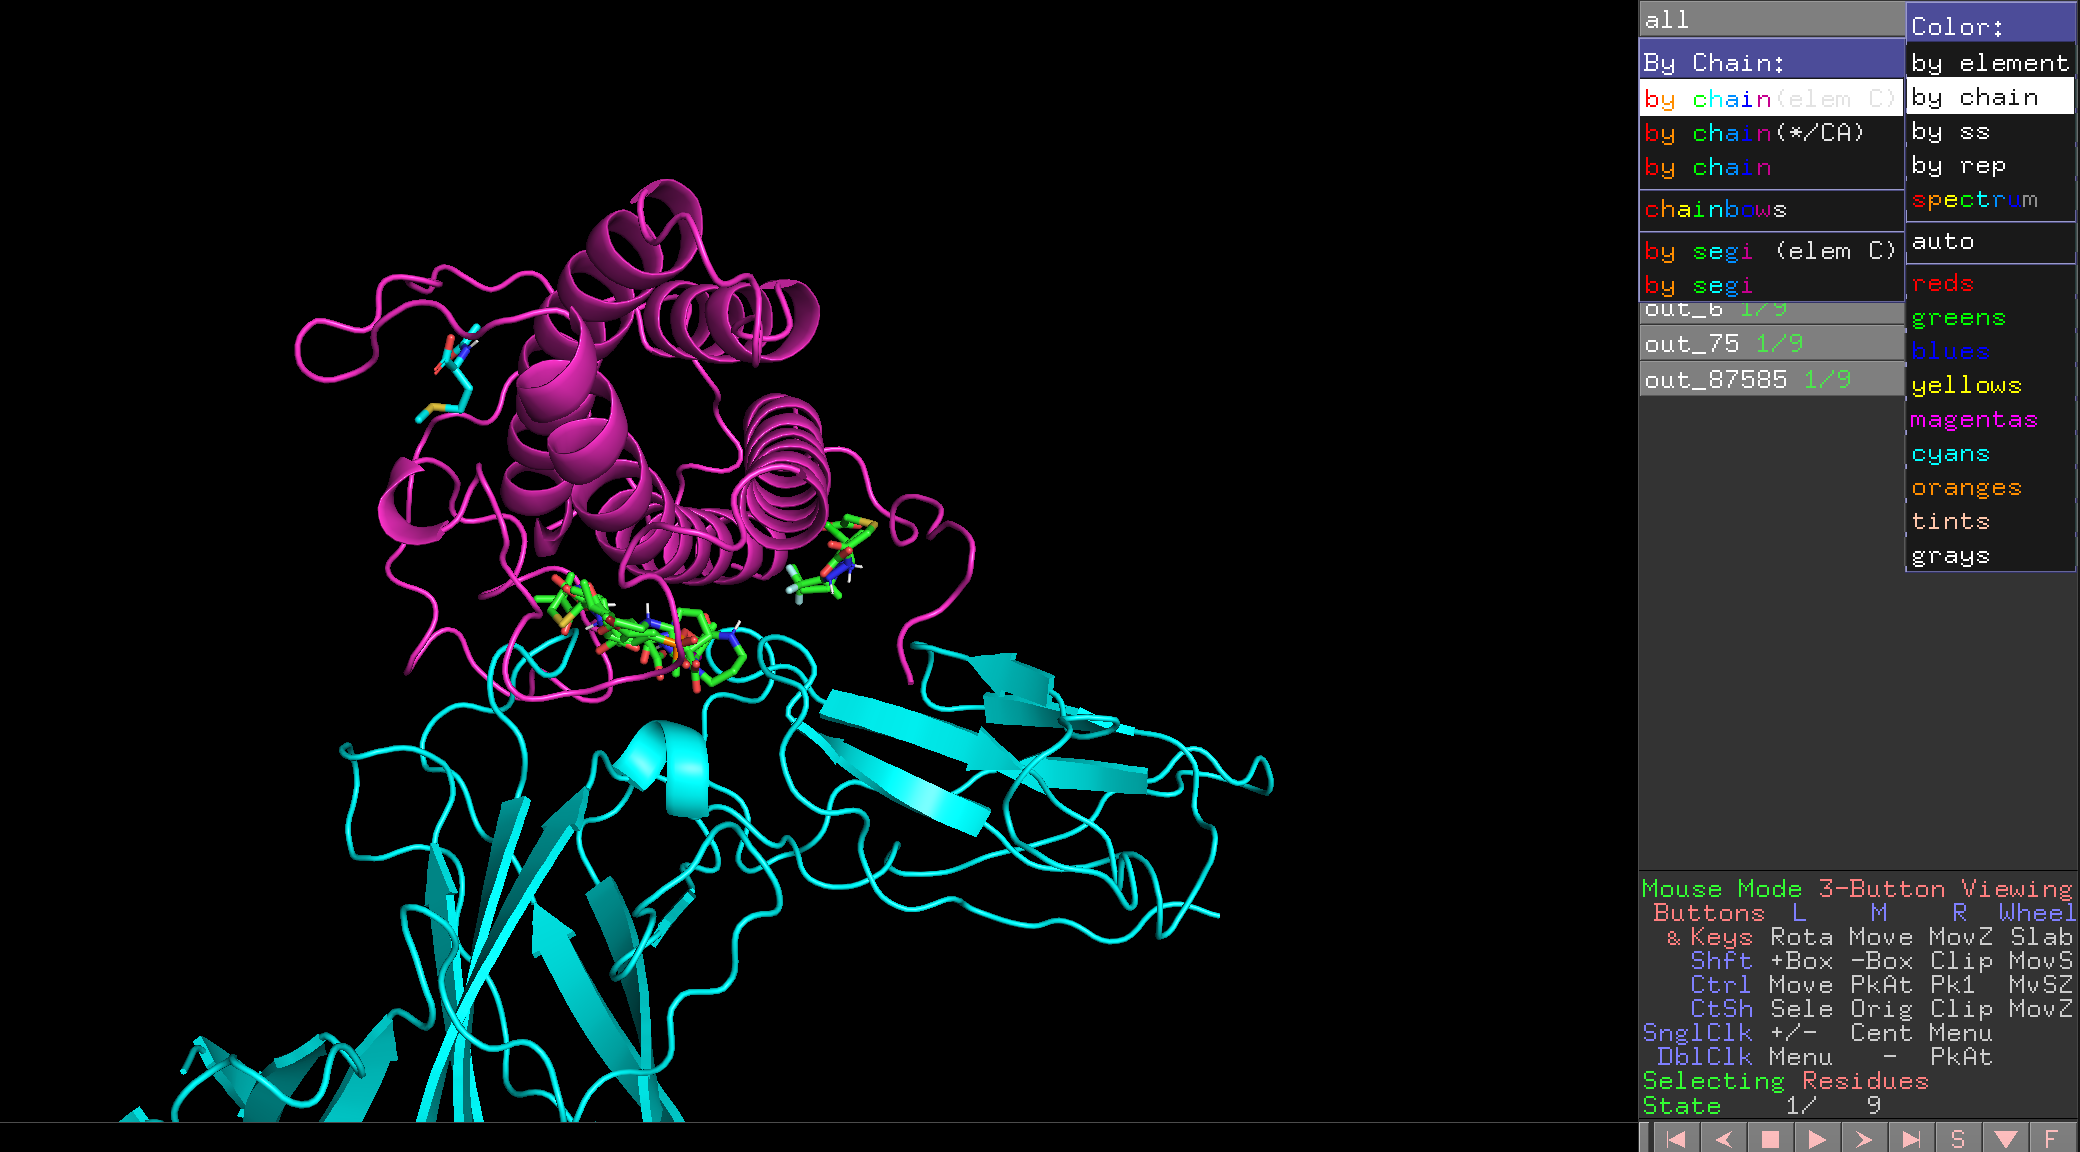
\includegraphics[width=0.45\textwidth]{figures/visualize_docking_pymol.png}
\caption{Visualization of the test docking output. In the lower right corner, it reads \code{State 1/9}. This means a maximum of 9 docking poses are available for the docked ligands, which can be navigated with the arrow keys.}
\label{fig:visualize_docking_pymol}
\end{figure}

The main point of the docking test here is to check if the ligands are mostly docked in the desired interface pocket. In case of substantially deviating results, the pocket size can be decreased, or another interface pocket can be selected altogether. After desirable results are ensured, the BSA between the test ligands and two proteins can be calculated for comparison, as well as their docking scores. The program \code{01\_vinatest\_analysis.ipynb} contains the analysis procedure. Executing all cells in said Jupyter Notebook should visualize the distribution of BSA and the docking score similar to the pocket analysis in \fref{fig:BSA_drugscore}. Note that the docking score here is in units of kcal/mol, and the lower the docking score, the stronger the expected binding affinity. From \fref{fig:BSA_dockingscore_vina}, it becomes apparent that ligand 1 has the lowest docking score and the largest BSA$_{min}$; thus, it is potentially the best PPI stabilizer candidate among the test ligands.

\begin{figure}[H]
\centering
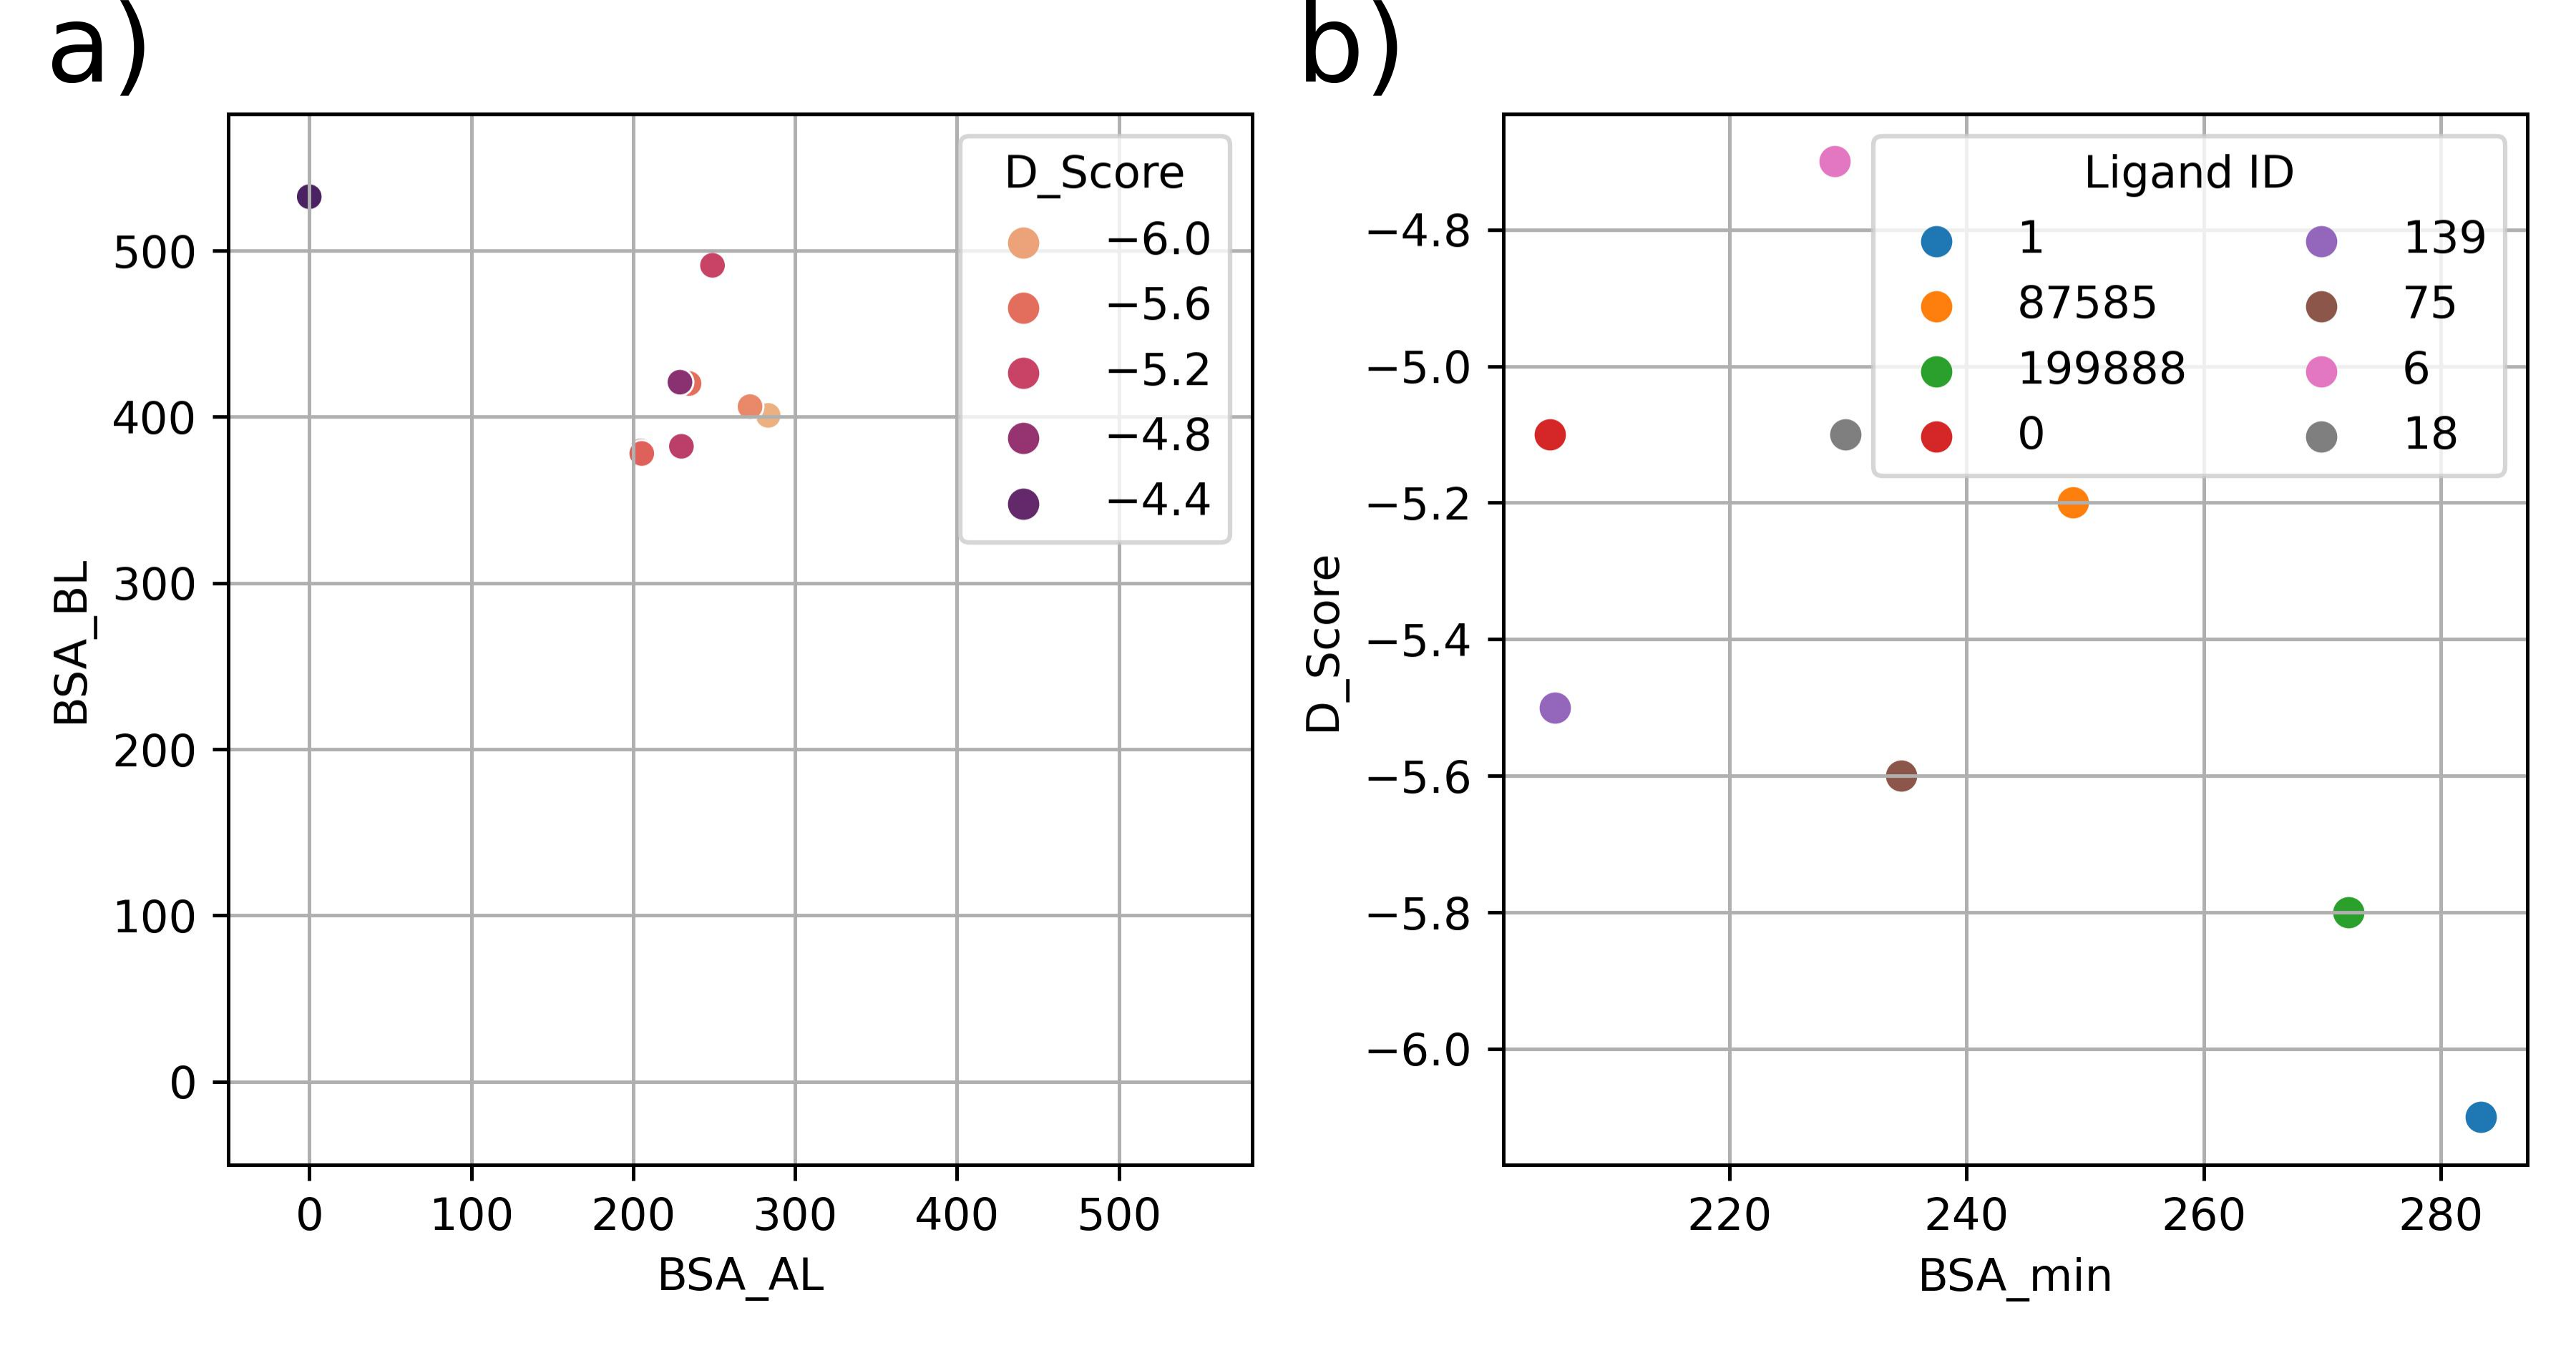
\includegraphics[width=0.45\textwidth]{figures/BSA_dockingscore_vina.png}
\caption{Visualization of the docking result from AutoDock Vina in terms of BSA and docking score.}
\label{fig:BSA_dockingscore_vina}
\end{figure}

The Jupyter Notebook also visualizes the docking poses using \code{nglview}. The resulting output of the visualization panel should look similar to \fref{fig:3hmx_ligand0001_visualisation_vina}. We can choose the ligand, and the ligand state can be changed by setting \code{L\_path} accordingly. Because calculating the BSA for a docking pose is relatively time-consuming, only the docking pose with the lowest docking score is analysed in the code.

\begin{figure}[H]
\centering
\includegraphics[width=0.45\textwidth]{figures/3hmx_ligand0001_visualisation_vina.png}
\caption{Visualization of the docking pose of the first docking mode of ligand 1 with a magnification of the ligand.}
\label{fig:3hmx_ligand0001_visualisation_vina}
\end{figure}



\subsubsection*{Large-Scale Screening with AutoDock-GPU}
Although docking with a few molecules using \code{vina} already yields good results, screening a larger ligand database has a higher chance of discovering a better PPIS candidate. With the confirmation that the obtained docking box can successfully dock the ligands at the protein-protein interface, large-scale ligand screening can continue using \code{autodock\_gpu}. Using a Nvidia RTX2080ti GPU enables a screening speed of up to 0.6 million compounds per week.\\
For docking, \code{autodock\_gpu} reads a set of grid parameter files, including \code{map}, \code{maps.fld}, \code{maps.xyz}. These files can be created via a ready-made \texttt{GPF} file called \code{hmx.gpf} that can be found in \code{04\_virtual\_screening/}. It mostly contains paths to crucially important files and some options that need to be set for the docking procedure. Curious users may inspect the file; however, changing its contents is not recommended. The \code{autogrid4} command can automatically generate all related files, given the \texttt{GPF} file and the receptor file. The required commands can be seen below. The respective map files should be generated in a separate folder for tidiness reasons.
\begin{lstlisting}[language=bash]
mkdir autogrid
cp -v ../03_docking_prep/hmx_B99990001.pdbqt hmx.gpf autogrid/
cd autogrid/
autogrid4 -p hmx.gpf
\end{lstlisting}
With the \texttt{MAP} files ready in \code{04\_virtual\_screening/autogrid/}, the ligands prepared in \code{02\_ligand\_pre/PDBQT/}, the next step is to generate a file for \code{autodock\_gpu} to perform automatic docking experiments, called \code{docking.dat} which contains the locations of the input and output files and the location of the \texttt{MAP} files. Creating the file \code{docking.dat} and the docking itself should not be absolved manually, instead a bash script \code{virtual\_screening.sh} downloadable from the online repository is supposed to take care of the procedure. The user should scrutinize the file and enure that the \code{autodock\_gpu} executable exists. The script also handles the directory infrastructure. Thus, output files can be found in the directory \code{04\_virtual\_screening/docking/}. Furthermore, the for-loop is automatically aborted after the first iteration if \code{virtual\_screening.sh} is executed as is for testing purposes. In case of a successful execution, the \code{break} statement can be commented out by inserting a \code{\#}. The following execution of \code{virtual\_screening.sh} will then try to dock all ligands saved in the specified directory.
\begin{lstlisting}[language=bash]
./virtual_screening.sh
\end{lstlisting}
The premier output of this docking process is \texttt{DLG} files and \texttt{XML} files for each docked ligand. The \texttt{DLG} file is the coordinate file, which is very similar to a \texttt{PDBQT} file format-wise only that each line is prefixed with a \code{DOCKED:}. The standard output to the terminal for a successful docking should look similar to the text below.
\begin{lstlisting}[showspaces=false]
Running Job #2224:
    Device: NVIDIA GeForce GTX 1080
    [...]
    [...]
    [...]
the best molecules of the last 4 * 5 generations, 42000 generations, or 1132076 evaluations:

Generations |  Evaluations |     Threshold    |  Average energy o...
------------+--------------+------------------+------------------...
          0 |          150 |232675.16 kcal/mol|    0.00 +/-    0...
          5 |        25110 |232675.16 kcal/mol|    0.00 +/-    0...
[...]
[...]
[...]
                        0.00 +/-    0.00 kcal/mol combined.
                     0 samples, best energy 232675.16 kcal/mol.
\end{lstlisting}
After the ligand screening, the results should be analysed like the test docking. In \code{04\_virtual\_screening}, a Jupyter Notebook can be found that contains the code for said analysis. At the beginning of the notebook \code{01\_GPUdock\_analysis.ipynb}, the docked ligand files are read, and the docking scores for the best state of each compound are saved and then plotted as a histogram. The resulting plot is saved and should look similar to \fref{fig:dockingscore_distribution_GPU}. Noticeably, only compounds with a score lower than 10 are plotted since many compounds might have scores magnitudes larger, skewing the distribution. 

\begin{figure}[H]
\centering
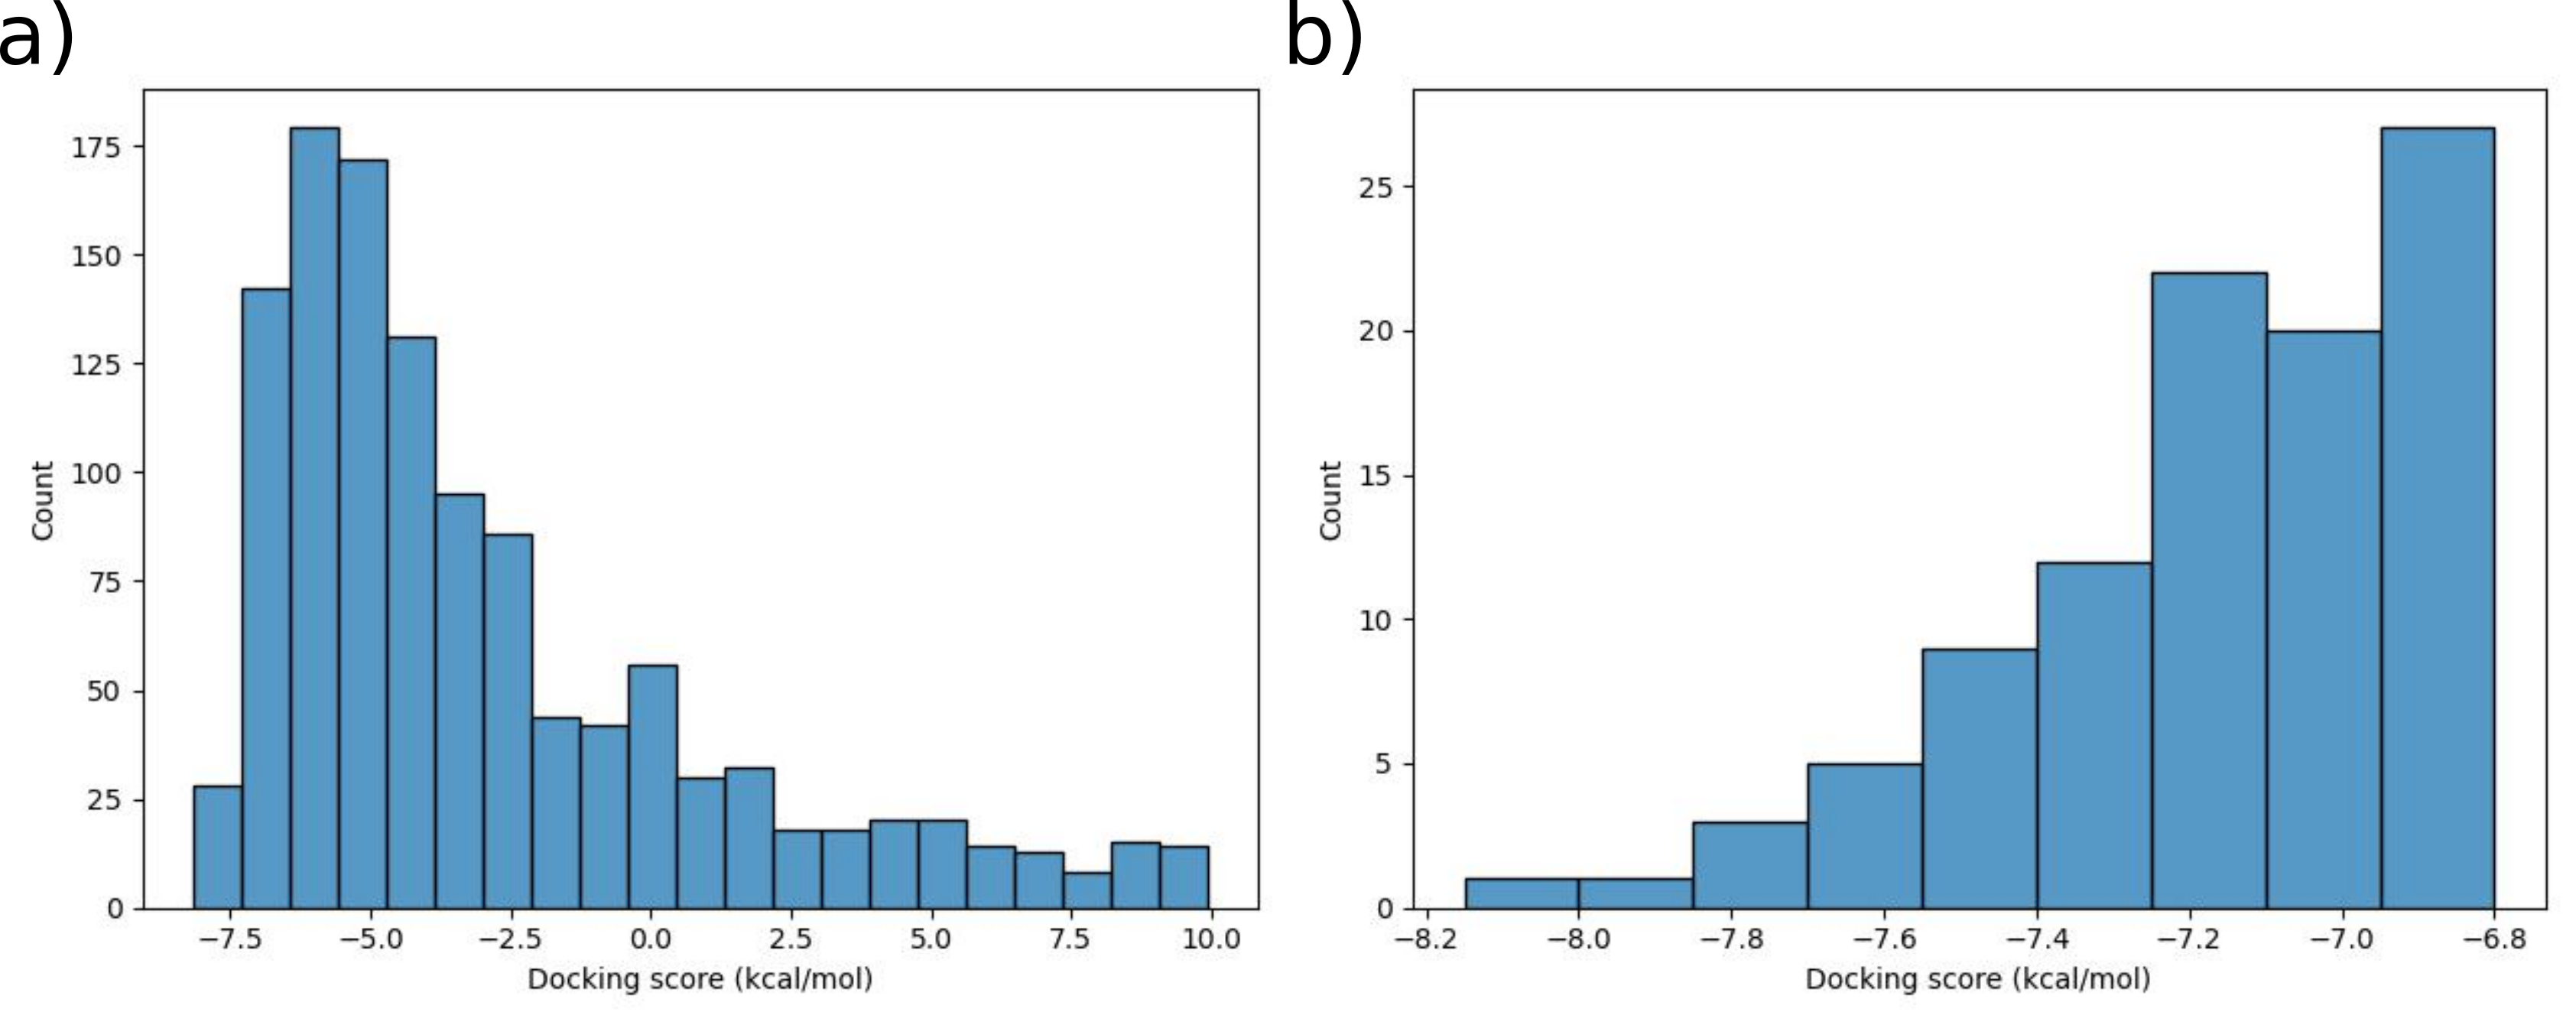
\includegraphics[width=0.45\textwidth]{figures/dockingscore_distribution_GPU.png}
\caption{Sub-distribution of docking score outputs from \code{autdock-gpu} by reading the best-scored docking pose of each ligand.}
\label{fig:dockingscore_distribution_GPU}
\end{figure}

The scoring of the compounds allows one to select the compounds. Herein, the 100 compounds with the lowest scores are picked for further processing. The notebook again features a histogram of their docking scores (see \fref{fig:dockingscore_distribution_GPU}). Then it converts them from \texttt{DLG} to \texttt{PDBQT} format followed by yet another conversion into \texttt{SMI}, \texttt{MOL2} and \texttt{PDB} format which is achieved by executing \code{convert.sh} from the notebook. For the conversion, \code{obabel} is used, and the script also relies on the correct directory structure and names. If the user customises any prior naming conventions, changes must be made to \code{convert.sh}. After both conversions, the well-known calculation of the BSA is conducted for the top compounds and is visualised in a previously described way. Again, this is done to quantify how well the ligands stay at the interface by calculating the buried surface area of protein A and protein B. An exemplary distribution of docking score, BSA$_{AL}$, and BSA$_{BL}$ are shown in \fref{fig:BSA_dockingscore_GPU}.

\begin{figure}[H]
\centering
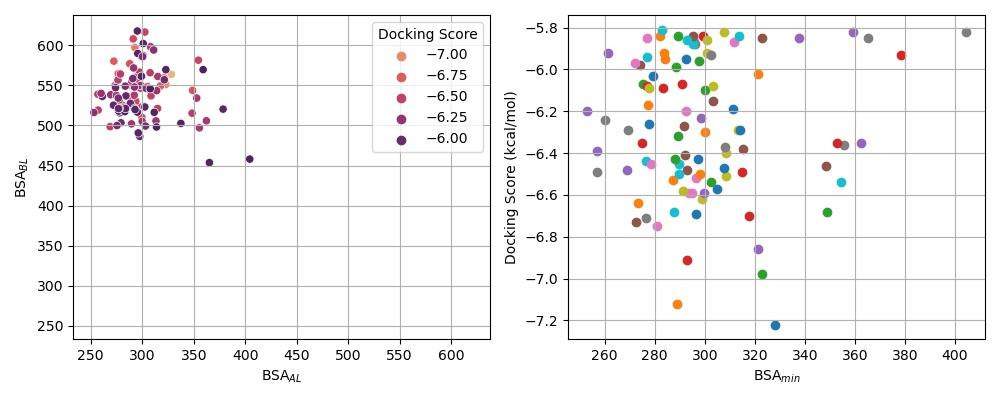
\includegraphics[width=0.45\textwidth]{figures/BSA_dockingscore_GPU.jpeg}
\caption{Data visualization of the protein-ligand BSA and docking score. On the left the distributions of BSA$_{AP}$ and BSA$_{BP}$ are shown of all detected pockets with color coded docking score. On the right the distribution of BSA$_{min}$ and the docking score of the interface ligand can be seen.}
\label{fig:BSA_dockingscore_GPU}
\end{figure}

Since a good PPI stabilizer must have a sufficiently high binding affinity to both proteins, a ligand should prevail with a high docking score and BSA$_{min}$. A mechanic offered by the python package \code{mplcursors} eases the selection process by enabling interactive plots. One cell in \code{01\_GPUdock\_analysis.ipynb} utilises this package to plot the same distribution shown in \fref{fig:BSA_dockingscore_GPU} with the difference, another window opens, and the ligand ID appears upon hovering over the data point with the cursor, as shown in \fref{fig:mplcursor_BSA_dockingscore}. 

\begin{figure}[H]
\centering
\includegraphics[width=0.45\textwidth]{figures/mplcursor_BSA_dockingscore.png}
\caption{Data visualization with \code{mplcursors}.}
\label{fig:mplcursor_BSA_dockingscore}
\end{figure}

Once a promising compound could be made out, its docking pose can be visualised via \code{nglview}. By setting the \code{L\_path} to the respective \texttt{PDB} output path in the respective cell, the ligand docking pose can be seen at the interface as shown in \fref{fig:3hmx_ligand0156_visualisation_GPU}.

\begin{figure}[H]
\centering
\includegraphics[width=0.45\textwidth]{figures/3hmx_ligand0156_visualisation_GPU.png}
\caption{Visualization of Ligand 0156 docked at the interface between protein A (blue) and protein B (red).}
\label{fig:3hmx_ligand0156_visualisation_GPU}
\end{figure}

The generated \texttt{SMI} files stored in \code{04\_virtual\_screening/SMI/} are used in the last step of the Jupyter Notebook. These files contain the SMILES string of each compound, which is unique to each compound (but not unique for each compound) and can be read by \texttt{RDKit} and used to search compounds in the ZINC20 database. Executing the respective cell in the Jupyter Notebook visualises the molecular graph of each compound in a \texttt{Pandas} Dataframe similar to \fref{fig:ligand0156_RDkit}. 

\begin{figure}[H]
\centering
\includegraphics[width=0.45\textwidth]{figures/ligand0156_RDkit.png}
\caption{Molecular graph of the docked compound 0156.}
\label{fig:ligand0156_RDkit}
\end{figure}

For some users, this can raise a \code{\_get\_adjustment} Attribute error that was mentioned in \code{TOY.ipynb} in \code{00\_install\_prep}. The bug fix described in the \code{TOY.ipynb} only takes effect after restarting the respective notebook (go to \code{kernel $\to$ Restart}). Apart from visualising the molecular graph, the SMILES string enables the user to easily browse the ZINC20 substance page (\url{zinc20.docking.org/substances/home/}) for the compound. In an actual scientific project, these compounds could be purchased from vendors conveniently listed on the website for experimental validation. The docking process is concluded with this step. The docked compounds can be further evaluated with MD simulations, or a more extensive screening can be conducted by increasing the number of ligands for GPU-docking before continuing.


\subsection*{Molecular Dynamics Simulation with GROMACS and MM/GBSA}
Regarding drug screening, the whole process can be imagined as a funnel that increases sensitivity with each step. The first step was prompting the ZINC20 database more or less arbitrarily to reduce the unfathomable amount of available chemical compounds by a large margin. The next step included the application of chemical criteria that the compounds should obey. Even though they were chosen arbitrarily in this exercise, they could incorporate empirical knowledge relevant to the system. The filtering was followed by the docking experiments, which assigned each compound a binding score and estimated the buried surface area. The sensitivity of these metrics is already quite high and facilitates the dismissal of many unsuitable compounds. Only two to five best-ranking compounds should be tested to further taper the funnel.\\
The next step is to conduct an MD simulation with GROMACS\cite{mark_abraham_2023_8134388} to investigate the dynamical properties of the protein-protein-ligand ternary complex as well as to estimate the binding free energy with  molecular mechanics generalized Born and surface area solvation (MM/GBSA).\cite{Wang2019} MM/GBSA is a middle ground between docking and free energy perturbation (FEP). While docking is fast, the results are unreliable; however, FEP calculations impose a ludicrous computational cost that cannot be covered on a large scale, especially with large ternary systems like the one investigated in this exercise. Therefore, MM/GBSA is the method of choice since it is especially suited for comparing the free energies of similar systems.



\subsubsection*{Ligand Paramterization and MD simulation}
The working directory contains five subfolders to keep things ordered: \code{\_exec}, \code{\_inp}, \code{\_output}, \code{\_sim}, and \code{\_trash}. The structure of these folders should not be changed since they are hard coded in downstream executables facilitating the MD simulations. 
\begin{itemize}
    \item \code{\_exec} contains binaries to be executed or distributed into the simulation directories.
    \item \code{\_inp} contains input files to be copied into the simulation directories, where they are usually modified or processed differently.
    \item \code{\_output} contains output files from analysis of the simulations, like plots or data tables with calculated results.
    \item \code{\_sim} contains the simulation directories. Herein, \code{\_sim} will contain one further subdirectory for each ligand in which the actual simulation runs will be conducted.
    \item \code{\_trash} contains seemingly unnecessary files. 'Seemingly' because deleted files tend to become necessary again after being deleted. Therefore, it is recommended not to use \code{mv} rather than \code{rm}. The contents of \code{\_trash} may be deleted in the distant future once their irrelevancy has manifested itself. 
\end{itemize}
The first step in simulating the ligands is to change the directory into \code{\_exec} and look into the \code{prep\_setup.sh} script. At the beginning of this program, some variables might need adjustment from the user. Most noticeably, \code{L\_ids} should be set to the ligand IDs found to be the best-ranked ones. As a reminder, ligands are ranked and selected in the prior step with \code{01\_GPUdock\_analysis.ipynb}. Anything else does not need to be changed as long as the user makes no unforeseen manual modifications. The variable declarations at the beginning of \code{prep\_setup.sh} should be checked when in doubt.\\ 
One of the tasks that \code{prep\_setup.sh} completes is to copy \code{prep\_and\_run.sh} in each ligand simulation directory and to modify them accordingly. \code{prep\_and\_run.sh} is the main executable and takes care of the parameterization of the ligands and the MD simulation itself. The whole process is quite complicated. Thus, the complex bash script consists of four different functions, which will not be printed in this exercise sheet but can be inspected by opening the file via \code{vi}. Nevertheless, the functions shall be briefly introduced.\\
\code{cp\_inp\_files} copies all necessary input files from the input directory into the current simulation directory and adjusts them for the respective ligand and receptor.\\
\code{gen\_params} calls some programs from \code{ambertools} and are used to generate custom parameters for the ligand molecules. This is necessary since these are likely not standard residues whose parameters are readily available in standard forcefields (like amino acids, water, and nucleic acids). There are several important output files of this function, like the \texttt{FRCMOD} file and \texttt{PDB} file of the complex.\\
\code{gen\_gmxtop} takes care of file compatibility. The output from \code{ambertools} is not suitable for \texttt{GROMACS} but only for the \texttt{AMBER} simulation package, which is not supported within this exercise. Therefore, the output files need to be converted to GROMACS compatible files, most importantly a working \code{topol.top}, which is the output of this function together with the respective \texttt{GRO} file.\\
\code{run\_gmx\_sims} sets up the simulation box and carries out the usual simulation sequence once the \texttt{TOP} and \texttt{GRO} files are present. Three repetitions are automatically conducted to calculate more reliable average properties in the analysis.\\
Natively, \code{gen\_gmxtop} and \code{run\_gmx\_sims} should be commented out with a \code{\#} at the end of the bash script, while \code{cp\_inp\_files} and \code{gen\_params} should be switched on. Uncommenting any other functions at this stage is unnecessary since the parametrization of the \texttt{MOL2} ligands from \code{obabel} often contain artifacts. Thus, executing the \code{prep\_and\_run.sh} in the respective ligand simulation directory often leads to a fatal error in the \code{antechamber} program similar to the one seen below.
\begin{lstlisting}
./prep_and_run.sh
[...]
/home/user123/micromamba3/envs/ppis/bin/to_be_dispatched/antechamber: Fatal Error!
Weird atomic valence (3) for atom (ID: 4, Name: C1).
       Possible open valence.
[...]
\end{lstlisting}
The error refers to valence charges assigned to the atoms of the ligand that do not fulfill the octet rule, usually caused by incorrect bond assignment at nitrogen atoms, double bonds, or aromatic rings. This problem requires manual correction via \texttt{PyMOL}. The file that needs to be corrected is the \texttt{MOL2} file in the \code{\_inp/} directory, e.g. \code{\_inp/1234.mol2}. 
\begin{lstlisting}[language=bash]
cd path/to/_inp/
pymol 1234.mol2
\end{lstlisting}
\texttt{PyMOL} has a tool for building and editing molecular structures. Most valence problems can be solved by fixing the hydrogen atoms of the structure and by adding the correct aromaticity. The procedure depicted in \fref{fig:ligandfix_manual_guide} can be used as guidance. Once the structure has been edited, overwrite the \texttt{MOL2} file of \code{1234.mol2} with the edited structure and execute \code{prep\_and\_run.sh} again.
\begin{lstlisting}[language=bash]
cd path/to/_exec/3hmx_1234/
./prep_and_run.sh
\end{lstlisting}
If the error persists, more editing might be attempted, or a different compound could be chosen for parametrization and simulation.

\begin{figure}[H]
\centering
\includegraphics[width=0.45\textwidth]{figures/ligandfix_manual_guide.png}
\caption{The process of editing a ligand with \texttt{PyMOL} is shown. The left picture shows how to access the \texttt{builder} menu. The two options \texttt{Fix H} and \texttt{Arom} were used in this specific example. The middle picture shows the ligand in its erroneous state. Hence, trying to generate parameters will fail. The right picture depicts the ligand state, resulting in a successful parametrization. Noticeably, aromaticity is added, as well as the explicit hydrogen atoms. Many other caveats could be wrong with a ligand, and some intuition is necessary for each fix.}
\label{fig:ligandfix_manual_guide}
\end{figure}

Once the parametrization is conducted successfully, the next function \code{gen\_gmxtop} can be switched on, and the prior two can be commented out. No user interaction is required; however, the function may show the following error, which can be ignored.
\begin{lstlisting}
Traceback (most recent call last):
  File "convertTOP_amb2gmx.py", line 596, in <module>
    perm_imp = get_permutations_4_wild(dihedral[0:4])
  File "convertTOP_amb2gmx.py", line 121, in get_permutations_4_wild
    temp_a = perm[2]
IndexError: list index out of range
\end{lstlisting}
The required \code{topol.top} and the \texttt{GRO} file should still be outputted. After asserting that these files exist, the last function of \code{prep\_and\_run.sh} may be executed. This function, \code{run\_gmx\_sims}, carries out the \texttt{GROMACS} simulations for the user. The \texttt{MDP} files are automatically copied from \code{\_inp/}, and the simulation output is automatically named. Each production run should be \SI{2}{\nano\second} long. The simulations can take some time since the system is quite large; however, three trajectories per compound should be created once they finish, named \code{prod\_center\_<REP>.xtc} containing 100 frames each. Once all simulations are finished, the trajectory analysis can start in the Jupyter Notebook \code{01\_analyse\_trajectory.ipynb} in the \code{\_exec} folder. The analysis of the trajectory is limited. However, some essential properties are computed that reveal the stability of the receptor complex. Firstly, the RMSD over the trajectory is measured for three compounds as shown in \fref{fig:6_rmsdvstime}. As a reminder, the RMSD is a measurement that reveals the average structural deviation from a reference structure for every time frame. Each run is depicted as an individual curve with the first frame of the trajectory as a reference. Considerable deviations from the reference could indicate substantial rearrangement of the receptor configuration, which should not happen given a stable receptor complex. 

\begin{figure}[H]
    \centering
    \includegraphics[width=0.45\textwidth]{figures/RMSD_vs_time.pdf}
    \caption{The RMSD is shown versus the simulation time. Each row corresponds to a different ligand, while the columns correspond to the two protein chains.}
    \label{fig:6_rmsdvstime}
\end{figure}

The RMSF is also calculated, giving the structural deviation as a time average per atom, which is more elucidating than the RMSD regarding structural integrity. Since stable atoms and stable conformation should exhibit a low RSMF value. In this notebook, three different ways to measure the RMSF are conducted. Firstly, the atom-wise RMSF is done to showcase the function rather than gain information. Secondly, the atomic RMSF is averaged per residue, revealing very mobile and less mobile residues. The expectation would be that residues in loops and unhindered parts of the protein have a considerable RMSF value, and those residues buried and in the interface have a lower RMSF value. The residue-wise RMSF is also calculated for three different compounds. However, the values are averaged over the two runs. The results can be seen in \fref{fig:6_rmsfresidues} with one curve per compound. Generally, the expectation that residues within the interface have lower RMSF is validated in this plot, and significant differences are visible between each compound's trajectories. For example, The curve of Ligand 0156 is generally higher than the other two for both protein chains, and the curve of compound 1258 seems to be most stable in general. The stable regions outside the interface cannot be attributed to compound stabilization but rather to the nature of the starting structure and its individual time development. The sampling might be insufficient to properly determine the most successful PPIS but it is sufficient for demonstrating the workflow in this exercise.

\begin{figure}[H]
    \centering
    \includegraphics[width=0.45\textwidth]{figures/RMSF_vs_resids.pdf}
    \caption{The residue-wise RMSF of the receptor is plotted with error bars shown as filled-in area. Although each curve follows a certain trend, the compounds largely differ concerning protein chain stability. The interface residues are shown as grey vertical lines.}
    \label{fig:6_rmsfresidues}
\end{figure}

The most important information is given in the last plot of the Jupyter Notebook, which consists of the atom-wise RMSF but only for the interfacial residues. Again, it can be seen that the stabilization differs between each compound. The ligands 1258 and 1306 are the best stabilizers for the interface residues (see \fref{fig:6_rmsfinterface}).

\begin{figure}[H]
    \centering
    \includegraphics[width=0.45\textwidth]{figures/RMSF_vs_iresids.pdf}
    \caption{The atomic RMSF for the interface residues for each protein chain. In both protein chains, compound 0156 seems the least performant, while the other two compete for the most stable interface. The error bars are again shown as filled-in areas with the same color shade.}
    \label{fig:6_rmsfinterface}
\end{figure}

In the prior exercise, checking the convergence of a system is covered for specific measurements and how a certain sampling sufficiency can be visualized. These tests are lacking here; the system is sizeable and would need much time to converge appropriately. The ambitious user can achieve convergence by increasing the number of steps in the respective \texttt{MDP} files and validating it using the methods in \fref{sec:ProteinSim}. 


\subsubsection*{Binding Free Energy Estimation with MM/GBSA}
The next step is to estimate the binding free energy with MM/GBSA to properly determine the most promising compound (the \code{ambertools} analysis function is called \code{MMPBSA.py} hence the name). The bash script \code{prep\_mmpbsa.sh} is another multipurpose bash script that handles many tasks simultaneously, given that the correct environment is activated. The main functionalities include the conversion of the GROMACS trajectory to an AMBER trajectory, its decomposition into the different system components (Chain A, Chain B, and the ligand), and its setting up of the directory structure for every selected compound. The ligands and receptor variables can be found at the beginning of \code{prep\_mmpbsa.sh} and must be adjusted accordingly before executing it.
\begin{lstlisting}[language=bash]
vi prep_mmpbsa.sh # alter script accordingly
./prep_mmpbsa.sh
\end{lstlisting}
After successful execution, all necessary files should already be transferred into the newly created subdirectories called \code{<REC-NAME>\_<LIG-ID>/}. One of these files is called \code{mmpbsa.sh}, which is used to estimate the binding free energies. Executing it will take a few hours and should result in a couple of \texttt{DAT} and \texttt{CSV} files, e.g. \code{AL\_output\_1.dat}. The progress can be tracked by using \code{grep} on the \texttt{MDOUT} file together with a line count command. Since MM/GBSA analyses the trajectory for the complex, the receptor, and the ligand, there are 300 frames. Thus, the calculations should be done once the following code outputs 300.
\begin{lstlisting}[language=bash]
grep 'NSTEP' _MMPBSA*.mdout.0 | wc -l
\end{lstlisting}
The \texttt{DAT} files contain the total binding free energy, and the \texttt{CSV} files contain the residue-wise decomposition of the free energy. The total amount of free energy should determine the optimal PPIS energy. The residue-wise decomposition can facilitate the lead optimization process, i.e., the knowledge-based modification of promising compounds to improve their efficacy. The Jupyter Notebook called \code{01\_visualise\_MMPBSA\_results.ipynb} in \code{06\_mmpbsa} offers guidance. The ligand's identifier must be adjusted before executing the specific cells. Also, the \code{ppis} environment needs to be activated.\\
The first plot of the notebook provides information about the total binding free energy from the MM/GBSA calculation. This notebook shows the total binding free energy for each compound run since only showing averages dilutes information. Good PPIS have small binding free energies to both protein chains while not favoring any of the two significantly (see \fref{fig:ligands_dGAvsdGB.png}).

\begin{figure}[H]
    \centering
    \includegraphics[width=0.45\textwidth]{figures/dGAvsdGB.pdf}
    \caption{Exemplary distribution of the binding free energies of 2 runs of 2 ligands. The free binding energy estimate for protein A is plotted on the x-axis, and the one for protein B is plotted on the y-axis. In this case none of the compounds seem promising.}
    \label{fig:ligands_dGAvsdGB.png}
\end{figure}
More helpful information is given in the second plot. Per default, the MM/GBSA calculation outputs a residue-wise free energy decomposition. This output is being read by the Jupyter Notebook and depicted per ligand and protein chain. Most residues do not interact significantly with the compound or contribute at all. However, the interface residues, depicted as grey, vertical lines, mainly contain non-zero contributions for both protein A and B (see \fref{fig:FE_ResidueDecomp}).
\begin{figure}[H]
    \centering
    \includegraphics[width=0.45\textwidth]{figures/FE_ResidueDecomp.pdf}
    \caption{Energy Decomposition of binding free energy. Each row belongs to a compound, and each column is the respective protein. The black vertical lines depict interfacial protein residues.}
    \label{fig:FE_ResidueDecomp}
\end{figure}
Last but not least, the Jupyter Notebook also visualizes the structure of the complex in a particular way that illuminates why specific residues facilitate and others inhibit the compound binding. In this visualization, all interfacial residues that facilitate binding are represented in white balls and sticks, while the unfavorable residues are shown as black balls and sticks. By inspecting the residues and their behavior over the trajectory, one may optimize the drug candidate further to interact more favorably with both proteins (see \fref{fig:3hmx_residueMMGBSA_visualisation}).
\begin{figure}[H]
    \centering
    \includegraphics[width=0.45\textwidth]{figures/3hmx_residueMMGBSA_visualisation.png}
    \caption{The complex is rendered with \code{nglview} once again, but this time, the residues of the interface are colored in by their contribution to the free energy of binding. In the zoomed-in section of the figure, one residue close by the ligand is interfering with the binding (black color), posing as a target for optimization.}
    \label{fig:3hmx_residueMMGBSA_visualisation}
\end{figure}
With the information provided in the plots of the Jupyter Notebook, one compound may be presented as the most promising PPIS. The compound should be presented structurally in a brief report, and the reasons why it outperforms its competition should be elaborated to outline the decision-making process.
%%% MMPBSA can result in error: bad atom type: i if for example iodide is present i the file. that should be reported here.


\subsection*{Conclusion}
This exercise presented an example workflow in a computer-assisted drug design application to identify a potential protein-protein interaction stabilizer from a database.
It involves many steps and several computer tools must be employed, ranging from the initial preparation of target-protein files to a detailed quantitative thermodynamic characterization of the drug-target complex.\\
Firstly, it is imperative to understand that the approach chosen in this exercise may not be universal or optimal for each PPI. Several steps including the MM/GBSA algorithms in \code{06\_mmpbsa/gb.in}, the number of frames in the \texttt{MDP} files and the scoring function in the molecular docking step may not be optimal.\\
A plausible outlook on such a research project could engulf a lead optimization guided by the MM/GBSA decomposition or higher precision free energy calculations, e.g., free energy perturbation. Experimentally, \textit{in-vitro} assays could be designed and conducted to determine the actual binding behavior of the drug candidates. Nevertheless, there are many choices to think about even after the virtual drug screening is successfully conducted. This complexity makes computer-assisted drug design an exciting and challenging task.


\section*{Author Contributions}
% ----- Author Contribution Information -----
% This section must describe the actual contributions of author
% Since this is an electronic-only journal, there is no length limit
% so we recommend describing what they actually did rather than simply categorizing them
% ----- ------ ------------ ----------- -----
\begin{itemize}
    \item Luis Vollmers
    \begin{itemize}\begingroup\fontsize{7pt}{7pt}\selectfont
        \item Wrote initial drafts for all exercises except \fref{sec:CompDrugDesign} and created corresponding materials in \githubrepository.
        \item Edited \fref{sec:CompDrugDesign} and adapted the materials for that exercise in \githubrepository.
        \item Wrote the drafts for all remaining sections.
        \item Created the bibliography.
        \item Wrote the pre-submission letter and handled correspondence.
        \item Edited the final draft.
    \end{itemize}\endgroup
    \item Shu-Yu Chen
    \begin{itemize}\begingroup\fontsize{7pt}{7pt}\selectfont
        \item Designed the course material after which \fref{sec:CompDrugDesign} was modeled.
        \item Wrote initial draft for \fref{sec:CompDrugDesign} and created the corresponding materials in \githubrepository.
        \item Edited the final draft.
    \end{itemize}\endgroup
    \item Maria Reif
    \begin{itemize}\begingroup\fontsize{7pt}{7pt}\selectfont
        \item Designed the university course material after which this article was modeled.
        \item Contributed to writing the draft, especially theoretical considerations in \fref{sec:freeEnerBind} and \fref{sec:freeEnerSolv}.
        \item Supervision and guidance of the whole process.
        \item Edited the final draft.
    \end{itemize}\endgroup
    \item Tristan Mauck
    \begin{itemize}\begingroup\fontsize{7pt}{7pt}\selectfont
        \item Wrote the model reports available in \githubrepository.
        \item Edited the final draft.
    \end{itemize}\endgroup
    \item Martin Zacharias 
    \begin{itemize}\begingroup\fontsize{7pt}{7pt}\selectfont
        \item Designed the university course material after which this article was modeled.
        \item Supervision and guidance of the whole process.
        \item Edited the final draft.
    \end{itemize}\endgroup
\end{itemize}
For a more detailed description of author contributions,
see the GitHub issue tracking and changelog at \githubrepository.

\section*{Author Information}
\makeorcid

\bibliography{bibliography.bib}

\end{document}
